\documentclass[a4paper]{book}
\usepackage{a4wide}
\usepackage{makeidx}
\usepackage{graphicx}
\usepackage{multicol}
\usepackage{float}
\usepackage{listings}
\usepackage{color}
\usepackage{textcomp}
\usepackage{alltt}
\usepackage{times}
\usepackage{ifpdf}
\ifpdf
\usepackage[pdftex,
            pagebackref=true,
            colorlinks=true,
            linkcolor=blue,
            unicode
           ]{hyperref}
\else
\usepackage[ps2pdf,
            pagebackref=true,
            colorlinks=true,
            linkcolor=blue,
            unicode
           ]{hyperref}
\usepackage{pspicture}
\fi
\usepackage[utf8]{inputenc}
\usepackage{doxygen}
\lstset{language=C++,inputencoding=utf8,basicstyle=\footnotesize,breaklines=true,breakatwhitespace=true,tabsize=8,numbers=left }
\makeindex
\setcounter{tocdepth}{3}
\renewcommand{\footrulewidth}{0.4pt}
\begin{document}
\hypersetup{pageanchor=false}
\begin{titlepage}
\vspace*{7cm}
\begin{center}
{\Large UNAT }\\
\vspace*{1cm}
{\large Generated by Doxygen 1.6.1}\\
\vspace*{0.5cm}
{\small Mon Dec 3 15:19:54 2018}\\
\end{center}
\end{titlepage}
\clearemptydoublepage
\pagenumbering{roman}
\tableofcontents
\clearemptydoublepage
\pagenumbering{arabic}
\hypersetup{pageanchor=true}
\chapter{Class Index}
\section{Class Hierarchy}
This inheritance list is sorted roughly, but not completely, alphabetically:\begin{DoxyCompactList}
\item \contentsline{section}{\_\-\_\-attribute\_\-\_\-}{\pageref{struct____attribute____}}{}
\item \contentsline{section}{Arrays}{\pageref{structArrays}}{}
\item \contentsline{section}{e2VParas}{\pageref{structe2VParas}}{}
\item \contentsline{section}{Iterator}{\pageref{classIterator}}{}
\begin{DoxyCompactList}
\item \contentsline{section}{MultiLevelBlockIterator}{\pageref{classMultiLevelBlockIterator}}{}
\end{DoxyCompactList}
\item \contentsline{section}{MLBFunParameters}{\pageref{structMLBFunParameters}}{}
\item \contentsline{section}{MLBParameters}{\pageref{structMLBParameters}}{}
\item \contentsline{section}{RlmpiInitializer}{\pageref{classRlmpiInitializer}}{}
\item \contentsline{section}{Schedule}{\pageref{structSchedule}}{}
\item \contentsline{section}{struct\_\-extensibleLABELArray}{\pageref{structstruct__extensibleLABELArray}}{}
\item \contentsline{section}{struct\_\-extensibleSCALARArray}{\pageref{structstruct__extensibleSCALARArray}}{}
\item \contentsline{section}{struct\_\-MLB\_\-graph}{\pageref{structstruct__MLB__graph}}{}
\item \contentsline{section}{topoArrays}{\pageref{structtopoArrays}}{}
\item \contentsline{section}{Topology}{\pageref{classTopology}}{}
\item \contentsline{section}{v2EParameters}{\pageref{structv2EParameters}}{}
\end{DoxyCompactList}

\chapter{Class Index}
\section{Class List}
Here are the classes, structs, unions and interfaces with brief descriptions\+:\begin{DoxyCompactList}
\item\contentsline{section}{\mbox{\hyperlink{struct____attribute____}{\+\_\+\+\_\+attribute\+\_\+\+\_\+}} }{\pageref{struct____attribute____}}{}
\item\contentsline{section}{\mbox{\hyperlink{structArrays}{Arrays}} }{\pageref{structArrays}}{}
\item\contentsline{section}{\mbox{\hyperlink{classUNAT_1_1DirectSegmentIterator}{U\+N\+A\+T\+::\+Direct\+Segment\+Iterator}} }{\pageref{classUNAT_1_1DirectSegmentIterator}}{}
\item\contentsline{section}{\mbox{\hyperlink{structDS__edge2VertexPara}{D\+S\+\_\+edge2\+Vertex\+Para}} }{\pageref{structDS__edge2VertexPara}}{}
\item\contentsline{section}{\mbox{\hyperlink{classUNAT_1_1Iterator}{U\+N\+A\+T\+::\+Iterator}} }{\pageref{classUNAT_1_1Iterator}}{}
\item\contentsline{section}{\mbox{\hyperlink{structRlmpiInfo}{Rlmpi\+Info}} }{\pageref{structRlmpiInfo}}{}
\item\contentsline{section}{\mbox{\hyperlink{classRlmpiInitializer}{Rlmpi\+Initializer}} }{\pageref{classRlmpiInitializer}}{}
\item\contentsline{section}{\mbox{\hyperlink{structSchedule}{Schedule}} }{\pageref{structSchedule}}{}
\item\contentsline{section}{\mbox{\hyperlink{structTable}{Table}} }{\pageref{structTable}}{}
\item\contentsline{section}{\mbox{\hyperlink{classUNAT_1_1Topology}{U\+N\+A\+T\+::\+Topology}} }{\pageref{classUNAT_1_1Topology}}{}
\end{DoxyCompactList}

\chapter{File Index}
\section{File List}
Here is a list of all files with brief descriptions:\begin{DoxyCompactList}
\item\contentsline{section}{iterator/\hyperlink{iterator_8H}{iterator.H} }{\pageref{iterator_8H}}{}
\item\contentsline{section}{iterator/\hyperlink{iterator__struct_8h}{iterator\_\-struct.h} }{\pageref{iterator__struct_8h}}{}
\item\contentsline{section}{iterator/multiLevelBlockIterator/\hyperlink{multiLevelBlockIterator_8C}{multiLevelBlockIterator.C} }{\pageref{multiLevelBlockIterator_8C}}{}
\item\contentsline{section}{iterator/multiLevelBlockIterator/\hyperlink{multiLevelBlockIterator_8H}{multiLevelBlockIterator.H} }{\pageref{multiLevelBlockIterator_8H}}{}
\item\contentsline{section}{iterator/multiLevelBlockIterator/BlockOrdering/\hyperlink{BlockOrdering_8c}{BlockOrdering.c} }{\pageref{BlockOrdering_8c}}{}
\item\contentsline{section}{iterator/multiLevelBlockIterator/BlockOrdering/\hyperlink{BlockOrdering_8h}{BlockOrdering.h} }{\pageref{BlockOrdering_8h}}{}
\item\contentsline{section}{iterator/multiLevelBlockIterator/BlockOrdering/\hyperlink{BlockOrderingSW_8c}{BlockOrderingSW.c} }{\pageref{BlockOrderingSW_8c}}{}
\item\contentsline{section}{iterator/multiLevelBlockIterator/BlockOrdering/\hyperlink{BOrderUtils_8c}{BOrderUtils.c} }{\pageref{BOrderUtils_8c}}{}
\item\contentsline{section}{iterator/multiLevelBlockIterator/BlockOrdering/\hyperlink{BOrderUtilsSW_8c}{BOrderUtilsSW.c} }{\pageref{BOrderUtilsSW_8c}}{}
\item\contentsline{section}{iterator/multiLevelBlockIterator/BlockOrdering/\hyperlink{BlockOrdering_2extensibleLabelArray_8h}{extensibleLabelArray.h} }{\pageref{BlockOrdering_2extensibleLabelArray_8h}}{}
\item\contentsline{section}{iterator/multiLevelBlockIterator/BlockOrdering/\hyperlink{metis_8h}{metis.h} (This file contains function prototypes and constant definitions for METIS )}{\pageref{metis_8h}}{}
\item\contentsline{section}{iterator/multiLevelBlockIterator/BlockOrdering/\hyperlink{timer_8h}{timer.h} }{\pageref{timer_8h}}{}
\item\contentsline{section}{iterator/multiLevelBlockIterator/edge2VertexIter/\hyperlink{edge2VertexIter__host_8c}{edge2VertexIter\_\-host.c} }{\pageref{edge2VertexIter__host_8c}}{}
\item\contentsline{section}{iterator/multiLevelBlockIterator/edge2VertexIter/\hyperlink{edge2VertexIter__host_8h}{edge2VertexIter\_\-host.h} }{\pageref{edge2VertexIter__host_8h}}{}
\item\contentsline{section}{iterator/multiLevelBlockIterator/edge2VertexIter/\hyperlink{edge2VertexIter__slave_8c}{edge2VertexIter\_\-slave.c} }{\pageref{edge2VertexIter__slave_8c}}{}
\item\contentsline{section}{iterator/multiLevelBlockIterator/edge2VertexIter/\hyperlink{edge2VertexIter__slave_8h}{edge2VertexIter\_\-slave.h} }{\pageref{edge2VertexIter__slave_8h}}{}
\item\contentsline{section}{iterator/multiLevelBlockIterator/edge2VertexIter/\hyperlink{funcPointer_8c}{funcPointer.c} }{\pageref{funcPointer_8c}}{}
\item\contentsline{section}{iterator/multiLevelBlockIterator/edge2VertexIter/\hyperlink{funcPointer_8h}{funcPointer.h} }{\pageref{funcPointer_8h}}{}
\item\contentsline{section}{iterator/multiLevelBlockIterator/edge2VertexIter/\hyperlink{userFunc__host_8c}{userFunc\_\-host.c} }{\pageref{userFunc__host_8c}}{}
\item\contentsline{section}{iterator/multiLevelBlockIterator/edge2VertexIter/\hyperlink{userFunc__host_8h}{userFunc\_\-host.h} }{\pageref{userFunc__host_8h}}{}
\item\contentsline{section}{iterator/multiLevelBlockIterator/edge2VertexIter/\hyperlink{userFunc__slave_8c}{userFunc\_\-slave.c} }{\pageref{userFunc__slave_8c}}{}
\item\contentsline{section}{iterator/multiLevelBlockIterator/edge2VertexIter/\hyperlink{userFunc__slave_8h}{userFunc\_\-slave.h} }{\pageref{userFunc__slave_8h}}{}
\item\contentsline{section}{iterator/multiLevelBlockIterator/extensibleArray/\hyperlink{extensibleLabelArray_8c}{extensibleLabelArray.c} }{\pageref{extensibleLabelArray_8c}}{}
\item\contentsline{section}{iterator/multiLevelBlockIterator/extensibleArray/\hyperlink{extensibleArray_2extensibleLabelArray_8h}{extensibleLabelArray.h} }{\pageref{extensibleArray_2extensibleLabelArray_8h}}{}
\item\contentsline{section}{iterator/multiLevelBlockIterator/extensibleArray/\hyperlink{extensibleLabelArraySW_8c}{extensibleLabelArraySW.c} }{\pageref{extensibleLabelArraySW_8c}}{}
\item\contentsline{section}{iterator/multiLevelBlockIterator/extensibleArray/\hyperlink{extensibleScalarArray_8c}{extensibleScalarArray.c} }{\pageref{extensibleScalarArray_8c}}{}
\item\contentsline{section}{iterator/multiLevelBlockIterator/extensibleArray/\hyperlink{extensibleScalarArray_8h}{extensibleScalarArray.h} }{\pageref{extensibleScalarArray_8h}}{}
\item\contentsline{section}{iterator/multiLevelBlockIterator/extensibleArray/\hyperlink{extensibleScalarArraySW_8c}{extensibleScalarArraySW.c} }{\pageref{extensibleScalarArraySW_8c}}{}
\item\contentsline{section}{iterator/multiLevelBlockIterator/vertex2EdgeIter/\hyperlink{userFuncUnsymm__host_8c}{userFuncUnsymm\_\-host.c} }{\pageref{userFuncUnsymm__host_8c}}{}
\item\contentsline{section}{iterator/multiLevelBlockIterator/vertex2EdgeIter/\hyperlink{userFuncUnsymm__host_8h}{userFuncUnsymm\_\-host.h} }{\pageref{userFuncUnsymm__host_8h}}{}
\item\contentsline{section}{iterator/multiLevelBlockIterator/vertex2EdgeIter/\hyperlink{userFuncUnsymm__slave_8c}{userFuncUnsymm\_\-slave.c} }{\pageref{userFuncUnsymm__slave_8c}}{}
\item\contentsline{section}{iterator/multiLevelBlockIterator/vertex2EdgeIter/\hyperlink{userFuncUnsymm__slave_8h}{userFuncUnsymm\_\-slave.h} }{\pageref{userFuncUnsymm__slave_8h}}{}
\item\contentsline{section}{iterator/multiLevelBlockIterator/vertex2EdgeIter/\hyperlink{vertex2EdgeIter__host_8c}{vertex2EdgeIter\_\-host.c} }{\pageref{vertex2EdgeIter__host_8c}}{}
\item\contentsline{section}{iterator/multiLevelBlockIterator/vertex2EdgeIter/\hyperlink{vertex2EdgeIter__host_8h}{vertex2EdgeIter\_\-host.h} }{\pageref{vertex2EdgeIter__host_8h}}{}
\item\contentsline{section}{iterator/multiLevelBlockIterator/vertex2EdgeIter/\hyperlink{vertex2EdgeIter__slave_8c}{vertex2EdgeIter\_\-slave.c} }{\pageref{vertex2EdgeIter__slave_8c}}{}
\item\contentsline{section}{RL\_\-MPI/\hyperlink{main_8cxx}{main.cxx} }{\pageref{main_8cxx}}{}
\item\contentsline{section}{RL\_\-MPI/\hyperlink{register_8C}{register.C} }{\pageref{register_8C}}{}
\item\contentsline{section}{RL\_\-MPI/\hyperlink{register_8H}{register.H} }{\pageref{register_8H}}{}
\item\contentsline{section}{RL\_\-MPI/\hyperlink{rlmpi_8c}{rlmpi.c} }{\pageref{rlmpi_8c}}{}
\item\contentsline{section}{RL\_\-MPI/\hyperlink{rlmpi_8h}{rlmpi.h} }{\pageref{rlmpi_8h}}{}
\item\contentsline{section}{RL\_\-MPI/\hyperlink{RlmpiInitializer_8cxx}{RlmpiInitializer.cxx} }{\pageref{RlmpiInitializer_8cxx}}{}
\item\contentsline{section}{RL\_\-MPI/\hyperlink{RlmpiInitializer_8hxx}{RlmpiInitializer.hxx} }{\pageref{RlmpiInitializer_8hxx}}{}
\item\contentsline{section}{RL\_\-MPI/\hyperlink{RlmpiSharedType_8h}{RlmpiSharedType.h} }{\pageref{RlmpiSharedType_8h}}{}
\item\contentsline{section}{RL\_\-MPI/\hyperlink{test_8c}{test.c} }{\pageref{test_8c}}{}
\item\contentsline{section}{test/multiLevelBlock/\hyperlink{test_8cpp}{test.cpp} }{\pageref{test_8cpp}}{}
\item\contentsline{section}{tools/\hyperlink{slaveUtils_8c}{slaveUtils.c} }{\pageref{slaveUtils_8c}}{}
\item\contentsline{section}{tools/\hyperlink{slaveUtils_8h}{slaveUtils.h} }{\pageref{slaveUtils_8h}}{}
\item\contentsline{section}{tools/\hyperlink{swMacro_8h}{swMacro.h} }{\pageref{swMacro_8h}}{}
\item\contentsline{section}{topology/\hyperlink{topology_8C}{topology.C} }{\pageref{topology_8C}}{}
\item\contentsline{section}{topology/\hyperlink{topology_8H}{topology.H} }{\pageref{topology_8H}}{}
\end{DoxyCompactList}

\chapter{Class Documentation}
\hypertarget{struct____attribute____}{}\section{\+\_\+\+\_\+attribute\+\_\+\+\_\+ Struct Reference}
\label{struct____attribute____}\index{\_\_attribute\_\_@{\_\_attribute\_\_}}


{\ttfamily \#include $<$Rlmpi\+Shared.\+h$>$}

\subsection*{Public Attributes}
\begin{DoxyCompactItemize}
\item 
\mbox{\hyperlink{include_2RlmpiShared_8h_af4148c3e44f31072c9b97e63e56bbde3}{s\+Real}} \mbox{\hyperlink{struct____attribute_____a9c5480ea0eef3f0de01687a9789fa444}{data}} \mbox{[}6\mbox{]}
\item 
unsigned \mbox{\hyperlink{struct____attribute_____a5520bd158c9067709c4581ee299ffb68}{res\+\_\+pos}}\+: 16
\item 
unsigned \mbox{\hyperlink{struct____attribute_____ab5ad54f2c28857af1bdac6584a3a1968}{src\+\_\+id}}\+: 8
\item 
unsigned \mbox{\hyperlink{struct____attribute_____abffd4da5aef1ba4854e7a81d14f86864}{dst\+\_\+id}}\+: 8
\item 
unsigned \mbox{\hyperlink{struct____attribute_____a0a82a10490ace7b38ae29ea0fb5fa7cd}{cva}}\+: 16
\item 
unsigned \mbox{\hyperlink{struct____attribute_____aba60a8b53615d05d77f736cb79afce4a}{cvb}}\+: 16
\item 
int \mbox{\hyperlink{struct____attribute_____aca7a5080435e36e62172756495e61b3b}{n\+P\+U\+TR}}
\item 
int \mbox{\hyperlink{struct____attribute_____a308fce32ca5f5670acc3f8d2073ab32d}{n\+G\+E\+TC}}
\item 
int \mbox{\hyperlink{struct____attribute_____a2d6aee77358153fff1c39b11895af6a2}{n\+G\+E\+T\+R\+\_\+\+P\+U\+TC}}
\item 
int \mbox{\hyperlink{struct____attribute_____a24f192574d106edbf269fa991e5b857e}{n\+Getr\+Same\+Row}}
\item 
int \mbox{\hyperlink{struct____attribute_____ac39c8684fd7d72438a65c2a17976e3b3}{n\+Putr\+Same\+Row}}
\item 
int \mbox{\hyperlink{struct____attribute_____a236aeba42ccf5515e5e3d75a98fadfbb}{n\+Getc\+Same\+Col}}
\item 
int \mbox{\hyperlink{struct____attribute_____a73b0f642eca0d1cd54815fd381727332}{n\+Putc\+Same\+Col}}
\item 
unsigned \mbox{\hyperlink{struct____attribute_____a215d68d123f74d9c49d41e3f21cc84ed}{indM}}\+: 16
\item 
unsigned \mbox{\hyperlink{struct____attribute_____aebaa365507fa4ca28d858516a653e5a7}{indP}}\+: 16
\end{DoxyCompactItemize}


\subsection{Member Data Documentation}
\mbox{\Hypertarget{struct____attribute_____a0a82a10490ace7b38ae29ea0fb5fa7cd}\label{struct____attribute_____a0a82a10490ace7b38ae29ea0fb5fa7cd}} 
\index{\_\_attribute\_\_@{\_\_attribute\_\_}!cva@{cva}}
\index{cva@{cva}!\_\_attribute\_\_@{\_\_attribute\_\_}}
\subsubsection{\texorpdfstring{cva}{cva}}
{\footnotesize\ttfamily unsigned \+\_\+\+\_\+attribute\+\_\+\+\_\+\+::cva}

\mbox{\Hypertarget{struct____attribute_____aba60a8b53615d05d77f736cb79afce4a}\label{struct____attribute_____aba60a8b53615d05d77f736cb79afce4a}} 
\index{\_\_attribute\_\_@{\_\_attribute\_\_}!cvb@{cvb}}
\index{cvb@{cvb}!\_\_attribute\_\_@{\_\_attribute\_\_}}
\subsubsection{\texorpdfstring{cvb}{cvb}}
{\footnotesize\ttfamily unsigned \+\_\+\+\_\+attribute\+\_\+\+\_\+\+::cvb}

\mbox{\Hypertarget{struct____attribute_____a9c5480ea0eef3f0de01687a9789fa444}\label{struct____attribute_____a9c5480ea0eef3f0de01687a9789fa444}} 
\index{\_\_attribute\_\_@{\_\_attribute\_\_}!data@{data}}
\index{data@{data}!\_\_attribute\_\_@{\_\_attribute\_\_}}
\subsubsection{\texorpdfstring{data}{data}}
{\footnotesize\ttfamily \mbox{\hyperlink{include_2RlmpiShared_8h_af4148c3e44f31072c9b97e63e56bbde3}{s\+Real}} \+\_\+\+\_\+attribute\+\_\+\+\_\+\+::data}

\mbox{\Hypertarget{struct____attribute_____abffd4da5aef1ba4854e7a81d14f86864}\label{struct____attribute_____abffd4da5aef1ba4854e7a81d14f86864}} 
\index{\_\_attribute\_\_@{\_\_attribute\_\_}!dst\_id@{dst\_id}}
\index{dst\_id@{dst\_id}!\_\_attribute\_\_@{\_\_attribute\_\_}}
\subsubsection{\texorpdfstring{dst\_id}{dst\_id}}
{\footnotesize\ttfamily unsigned \+\_\+\+\_\+attribute\+\_\+\+\_\+\+::dst\+\_\+id}

\mbox{\Hypertarget{struct____attribute_____a215d68d123f74d9c49d41e3f21cc84ed}\label{struct____attribute_____a215d68d123f74d9c49d41e3f21cc84ed}} 
\index{\_\_attribute\_\_@{\_\_attribute\_\_}!indM@{indM}}
\index{indM@{indM}!\_\_attribute\_\_@{\_\_attribute\_\_}}
\subsubsection{\texorpdfstring{indM}{indM}}
{\footnotesize\ttfamily unsigned \+\_\+\+\_\+attribute\+\_\+\+\_\+\+::indM}

\mbox{\Hypertarget{struct____attribute_____aebaa365507fa4ca28d858516a653e5a7}\label{struct____attribute_____aebaa365507fa4ca28d858516a653e5a7}} 
\index{\_\_attribute\_\_@{\_\_attribute\_\_}!indP@{indP}}
\index{indP@{indP}!\_\_attribute\_\_@{\_\_attribute\_\_}}
\subsubsection{\texorpdfstring{indP}{indP}}
{\footnotesize\ttfamily unsigned \+\_\+\+\_\+attribute\+\_\+\+\_\+\+::indP}

\mbox{\Hypertarget{struct____attribute_____a308fce32ca5f5670acc3f8d2073ab32d}\label{struct____attribute_____a308fce32ca5f5670acc3f8d2073ab32d}} 
\index{\_\_attribute\_\_@{\_\_attribute\_\_}!nGETC@{nGETC}}
\index{nGETC@{nGETC}!\_\_attribute\_\_@{\_\_attribute\_\_}}
\subsubsection{\texorpdfstring{nGETC}{nGETC}}
{\footnotesize\ttfamily int \+\_\+\+\_\+attribute\+\_\+\+\_\+\+::n\+G\+E\+TC}

\mbox{\Hypertarget{struct____attribute_____a236aeba42ccf5515e5e3d75a98fadfbb}\label{struct____attribute_____a236aeba42ccf5515e5e3d75a98fadfbb}} 
\index{\_\_attribute\_\_@{\_\_attribute\_\_}!nGetcSameCol@{nGetcSameCol}}
\index{nGetcSameCol@{nGetcSameCol}!\_\_attribute\_\_@{\_\_attribute\_\_}}
\subsubsection{\texorpdfstring{nGetcSameCol}{nGetcSameCol}}
{\footnotesize\ttfamily int \+\_\+\+\_\+attribute\+\_\+\+\_\+\+::n\+Getc\+Same\+Col}

\mbox{\Hypertarget{struct____attribute_____a2d6aee77358153fff1c39b11895af6a2}\label{struct____attribute_____a2d6aee77358153fff1c39b11895af6a2}} 
\index{\_\_attribute\_\_@{\_\_attribute\_\_}!nGETR\_PUTC@{nGETR\_PUTC}}
\index{nGETR\_PUTC@{nGETR\_PUTC}!\_\_attribute\_\_@{\_\_attribute\_\_}}
\subsubsection{\texorpdfstring{nGETR\_PUTC}{nGETR\_PUTC}}
{\footnotesize\ttfamily int \+\_\+\+\_\+attribute\+\_\+\+\_\+\+::n\+G\+E\+T\+R\+\_\+\+P\+U\+TC}

\mbox{\Hypertarget{struct____attribute_____a24f192574d106edbf269fa991e5b857e}\label{struct____attribute_____a24f192574d106edbf269fa991e5b857e}} 
\index{\_\_attribute\_\_@{\_\_attribute\_\_}!nGetrSameRow@{nGetrSameRow}}
\index{nGetrSameRow@{nGetrSameRow}!\_\_attribute\_\_@{\_\_attribute\_\_}}
\subsubsection{\texorpdfstring{nGetrSameRow}{nGetrSameRow}}
{\footnotesize\ttfamily int \+\_\+\+\_\+attribute\+\_\+\+\_\+\+::n\+Getr\+Same\+Row}

\mbox{\Hypertarget{struct____attribute_____a73b0f642eca0d1cd54815fd381727332}\label{struct____attribute_____a73b0f642eca0d1cd54815fd381727332}} 
\index{\_\_attribute\_\_@{\_\_attribute\_\_}!nPutcSameCol@{nPutcSameCol}}
\index{nPutcSameCol@{nPutcSameCol}!\_\_attribute\_\_@{\_\_attribute\_\_}}
\subsubsection{\texorpdfstring{nPutcSameCol}{nPutcSameCol}}
{\footnotesize\ttfamily int \+\_\+\+\_\+attribute\+\_\+\+\_\+\+::n\+Putc\+Same\+Col}

\mbox{\Hypertarget{struct____attribute_____aca7a5080435e36e62172756495e61b3b}\label{struct____attribute_____aca7a5080435e36e62172756495e61b3b}} 
\index{\_\_attribute\_\_@{\_\_attribute\_\_}!nPUTR@{nPUTR}}
\index{nPUTR@{nPUTR}!\_\_attribute\_\_@{\_\_attribute\_\_}}
\subsubsection{\texorpdfstring{nPUTR}{nPUTR}}
{\footnotesize\ttfamily int \+\_\+\+\_\+attribute\+\_\+\+\_\+\+::n\+P\+U\+TR}

\mbox{\Hypertarget{struct____attribute_____ac39c8684fd7d72438a65c2a17976e3b3}\label{struct____attribute_____ac39c8684fd7d72438a65c2a17976e3b3}} 
\index{\_\_attribute\_\_@{\_\_attribute\_\_}!nPutrSameRow@{nPutrSameRow}}
\index{nPutrSameRow@{nPutrSameRow}!\_\_attribute\_\_@{\_\_attribute\_\_}}
\subsubsection{\texorpdfstring{nPutrSameRow}{nPutrSameRow}}
{\footnotesize\ttfamily int \+\_\+\+\_\+attribute\+\_\+\+\_\+\+::n\+Putr\+Same\+Row}

\mbox{\Hypertarget{struct____attribute_____a5520bd158c9067709c4581ee299ffb68}\label{struct____attribute_____a5520bd158c9067709c4581ee299ffb68}} 
\index{\_\_attribute\_\_@{\_\_attribute\_\_}!res\_pos@{res\_pos}}
\index{res\_pos@{res\_pos}!\_\_attribute\_\_@{\_\_attribute\_\_}}
\subsubsection{\texorpdfstring{res\_pos}{res\_pos}}
{\footnotesize\ttfamily unsigned \+\_\+\+\_\+attribute\+\_\+\+\_\+\+::res\+\_\+pos}

\mbox{\Hypertarget{struct____attribute_____ab5ad54f2c28857af1bdac6584a3a1968}\label{struct____attribute_____ab5ad54f2c28857af1bdac6584a3a1968}} 
\index{\_\_attribute\_\_@{\_\_attribute\_\_}!src\_id@{src\_id}}
\index{src\_id@{src\_id}!\_\_attribute\_\_@{\_\_attribute\_\_}}
\subsubsection{\texorpdfstring{src\_id}{src\_id}}
{\footnotesize\ttfamily unsigned \+\_\+\+\_\+attribute\+\_\+\+\_\+\+::src\+\_\+id}



The documentation for this struct was generated from the following files\+:\begin{DoxyCompactItemize}
\item 
C\+:/\+Users/lenovo/\+Documents/\+Work/\+U\+N\+A\+T/include/\mbox{\hyperlink{include_2RlmpiShared_8h}{Rlmpi\+Shared.\+h}}\item 
C\+:/\+Users/lenovo/\+Documents/\+Work/\+U\+N\+A\+T/include/\mbox{\hyperlink{include_2RlmpiSharedType_8h}{Rlmpi\+Shared\+Type.\+h}}\end{DoxyCompactItemize}

\hypertarget{structArrays}{}\section{Arrays Struct Reference}
\label{structArrays}\index{Arrays@{Arrays}}


{\ttfamily \#include $<$iterator.\+h$>$}

\subsection*{Public Attributes}
\begin{DoxyCompactItemize}
\item 
\mbox{\hyperlink{include_2swMacro_8h_a4ce60b1aa82e56b7372553a6a5bf2c0b}{sw\+Float}} $\ast$$\ast$ \mbox{\hyperlink{structArrays_acc1c5c8b920ed82b661c62dae59c1d87}{float\+Arrays}}
\item 
\mbox{\hyperlink{include_2swMacro_8h_a113cf5f6b5377cdf3fac6aa4e443e9aa}{sw\+Int}} $\ast$$\ast$ \mbox{\hyperlink{structArrays_a3b8e8309d07651cb70a0a694855b804f}{int\+Arrays}}
\item 
\mbox{\hyperlink{include_2swMacro_8h_a113cf5f6b5377cdf3fac6aa4e443e9aa}{sw\+Int}} $\ast$ \mbox{\hyperlink{structArrays_a0ea463f279710afff06ffd4856406338}{f\+Array\+Dims}}
\item 
\mbox{\hyperlink{include_2swMacro_8h_a113cf5f6b5377cdf3fac6aa4e443e9aa}{sw\+Int}} $\ast$ \mbox{\hyperlink{structArrays_ac5691bcdd36e5def106b308f553ef714}{i\+Array\+Dims}}
\item 
\mbox{\hyperlink{include_2swMacro_8h_a113cf5f6b5377cdf3fac6aa4e443e9aa}{sw\+Int}} $\ast$ \mbox{\hyperlink{structArrays_a6bbf2ee6da277e3e2c780689fef08768}{f\+Array\+In\+Out}}
\item 
\mbox{\hyperlink{include_2swMacro_8h_a113cf5f6b5377cdf3fac6aa4e443e9aa}{sw\+Int}} $\ast$ \mbox{\hyperlink{structArrays_a0ff37b5ccb44cb2a3c6929764ddc2abe}{i\+Array\+In\+Out}}
\item 
\mbox{\hyperlink{include_2swMacro_8h_a113cf5f6b5377cdf3fac6aa4e443e9aa}{sw\+Int}} \mbox{\hyperlink{structArrays_a7ca77e28c268df2e7cb626afbeb005df}{f\+Array\+Num}}
\item 
\mbox{\hyperlink{include_2swMacro_8h_a113cf5f6b5377cdf3fac6aa4e443e9aa}{sw\+Int}} \mbox{\hyperlink{structArrays_a22a0a6af8c0a698bc7840bf1e9837db9}{i\+Array\+Num}}
\item 
\mbox{\hyperlink{include_2swMacro_8h_a113cf5f6b5377cdf3fac6aa4e443e9aa}{sw\+Int}} \mbox{\hyperlink{structArrays_a0f0308c0b53408426cfc6d036f9f72d0}{f\+Array\+Sizes}}
\item 
\mbox{\hyperlink{include_2swMacro_8h_a113cf5f6b5377cdf3fac6aa4e443e9aa}{sw\+Int}} \mbox{\hyperlink{structArrays_af5b71d24c66f1248b65dabc348773efa}{i\+Array\+Sizes}}
\end{DoxyCompactItemize}


\subsection{Member Data Documentation}
\mbox{\Hypertarget{structArrays_a0ea463f279710afff06ffd4856406338}\label{structArrays_a0ea463f279710afff06ffd4856406338}} 
\index{Arrays@{Arrays}!fArrayDims@{fArrayDims}}
\index{fArrayDims@{fArrayDims}!Arrays@{Arrays}}
\subsubsection{\texorpdfstring{fArrayDims}{fArrayDims}}
{\footnotesize\ttfamily \mbox{\hyperlink{include_2swMacro_8h_a113cf5f6b5377cdf3fac6aa4e443e9aa}{sw\+Int}} $\ast$ Arrays\+::f\+Array\+Dims}

\mbox{\Hypertarget{structArrays_a6bbf2ee6da277e3e2c780689fef08768}\label{structArrays_a6bbf2ee6da277e3e2c780689fef08768}} 
\index{Arrays@{Arrays}!fArrayInOut@{fArrayInOut}}
\index{fArrayInOut@{fArrayInOut}!Arrays@{Arrays}}
\subsubsection{\texorpdfstring{fArrayInOut}{fArrayInOut}}
{\footnotesize\ttfamily \mbox{\hyperlink{include_2swMacro_8h_a113cf5f6b5377cdf3fac6aa4e443e9aa}{sw\+Int}} $\ast$ Arrays\+::f\+Array\+In\+Out}

\mbox{\Hypertarget{structArrays_a7ca77e28c268df2e7cb626afbeb005df}\label{structArrays_a7ca77e28c268df2e7cb626afbeb005df}} 
\index{Arrays@{Arrays}!fArrayNum@{fArrayNum}}
\index{fArrayNum@{fArrayNum}!Arrays@{Arrays}}
\subsubsection{\texorpdfstring{fArrayNum}{fArrayNum}}
{\footnotesize\ttfamily \mbox{\hyperlink{include_2swMacro_8h_a113cf5f6b5377cdf3fac6aa4e443e9aa}{sw\+Int}} Arrays\+::f\+Array\+Num}

\mbox{\Hypertarget{structArrays_a0f0308c0b53408426cfc6d036f9f72d0}\label{structArrays_a0f0308c0b53408426cfc6d036f9f72d0}} 
\index{Arrays@{Arrays}!fArraySizes@{fArraySizes}}
\index{fArraySizes@{fArraySizes}!Arrays@{Arrays}}
\subsubsection{\texorpdfstring{fArraySizes}{fArraySizes}}
{\footnotesize\ttfamily \mbox{\hyperlink{include_2swMacro_8h_a113cf5f6b5377cdf3fac6aa4e443e9aa}{sw\+Int}} Arrays\+::f\+Array\+Sizes}

\mbox{\Hypertarget{structArrays_acc1c5c8b920ed82b661c62dae59c1d87}\label{structArrays_acc1c5c8b920ed82b661c62dae59c1d87}} 
\index{Arrays@{Arrays}!floatArrays@{floatArrays}}
\index{floatArrays@{floatArrays}!Arrays@{Arrays}}
\subsubsection{\texorpdfstring{floatArrays}{floatArrays}}
{\footnotesize\ttfamily \mbox{\hyperlink{include_2swMacro_8h_a4ce60b1aa82e56b7372553a6a5bf2c0b}{sw\+Float}} $\ast$$\ast$ Arrays\+::float\+Arrays}

\mbox{\Hypertarget{structArrays_ac5691bcdd36e5def106b308f553ef714}\label{structArrays_ac5691bcdd36e5def106b308f553ef714}} 
\index{Arrays@{Arrays}!iArrayDims@{iArrayDims}}
\index{iArrayDims@{iArrayDims}!Arrays@{Arrays}}
\subsubsection{\texorpdfstring{iArrayDims}{iArrayDims}}
{\footnotesize\ttfamily \mbox{\hyperlink{include_2swMacro_8h_a113cf5f6b5377cdf3fac6aa4e443e9aa}{sw\+Int}} $\ast$ Arrays\+::i\+Array\+Dims}

\mbox{\Hypertarget{structArrays_a0ff37b5ccb44cb2a3c6929764ddc2abe}\label{structArrays_a0ff37b5ccb44cb2a3c6929764ddc2abe}} 
\index{Arrays@{Arrays}!iArrayInOut@{iArrayInOut}}
\index{iArrayInOut@{iArrayInOut}!Arrays@{Arrays}}
\subsubsection{\texorpdfstring{iArrayInOut}{iArrayInOut}}
{\footnotesize\ttfamily \mbox{\hyperlink{include_2swMacro_8h_a113cf5f6b5377cdf3fac6aa4e443e9aa}{sw\+Int}} $\ast$ Arrays\+::i\+Array\+In\+Out}

\mbox{\Hypertarget{structArrays_a22a0a6af8c0a698bc7840bf1e9837db9}\label{structArrays_a22a0a6af8c0a698bc7840bf1e9837db9}} 
\index{Arrays@{Arrays}!iArrayNum@{iArrayNum}}
\index{iArrayNum@{iArrayNum}!Arrays@{Arrays}}
\subsubsection{\texorpdfstring{iArrayNum}{iArrayNum}}
{\footnotesize\ttfamily \mbox{\hyperlink{include_2swMacro_8h_a113cf5f6b5377cdf3fac6aa4e443e9aa}{sw\+Int}} Arrays\+::i\+Array\+Num}

\mbox{\Hypertarget{structArrays_af5b71d24c66f1248b65dabc348773efa}\label{structArrays_af5b71d24c66f1248b65dabc348773efa}} 
\index{Arrays@{Arrays}!iArraySizes@{iArraySizes}}
\index{iArraySizes@{iArraySizes}!Arrays@{Arrays}}
\subsubsection{\texorpdfstring{iArraySizes}{iArraySizes}}
{\footnotesize\ttfamily \mbox{\hyperlink{include_2swMacro_8h_a113cf5f6b5377cdf3fac6aa4e443e9aa}{sw\+Int}} Arrays\+::i\+Array\+Sizes}

\mbox{\Hypertarget{structArrays_a3b8e8309d07651cb70a0a694855b804f}\label{structArrays_a3b8e8309d07651cb70a0a694855b804f}} 
\index{Arrays@{Arrays}!intArrays@{intArrays}}
\index{intArrays@{intArrays}!Arrays@{Arrays}}
\subsubsection{\texorpdfstring{intArrays}{intArrays}}
{\footnotesize\ttfamily \mbox{\hyperlink{include_2swMacro_8h_a113cf5f6b5377cdf3fac6aa4e443e9aa}{sw\+Int}} $\ast$$\ast$ Arrays\+::int\+Arrays}



The documentation for this struct was generated from the following file\+:\begin{DoxyCompactItemize}
\item 
C\+:/\+Users/lenovo/\+Documents/\+Work/\+U\+N\+A\+T/include/\mbox{\hyperlink{include_2iterator_8h}{iterator.\+h}}\end{DoxyCompactItemize}

\hypertarget{structe2VParas}{
\section{e2VParas Struct Reference}
\label{structe2VParas}\index{e2VParas@{e2VParas}}
}


{\ttfamily \#include $<$edge2VertexIter\_\-host.h$>$}\subsection*{Public Attributes}
\begin{DoxyCompactItemize}
\item 
\hyperlink{structMLBParameters}{MLBParameters} $\ast$ \hyperlink{structe2VParas_adbc014a3c6f625888247c1c8f2d13ecc}{MLBParas}
\item 
\hyperlink{swMacro_8h_a4ce60b1aa82e56b7372553a6a5bf2c0b}{swFloat} $\ast$ \hyperlink{structe2VParas_a6036626301d5765def554aadddea0ae3}{lower}
\item 
\hyperlink{swMacro_8h_a4ce60b1aa82e56b7372553a6a5bf2c0b}{swFloat} $\ast$ \hyperlink{structe2VParas_aa47e1f24e424418952a31e4d943b961e}{upper}
\item 
\hyperlink{swMacro_8h_a4ce60b1aa82e56b7372553a6a5bf2c0b}{swFloat} $\ast$ \hyperlink{structe2VParas_a5d3d9444ff7cd409f4c555110ce4d892}{x}
\item 
\hyperlink{swMacro_8h_a4ce60b1aa82e56b7372553a6a5bf2c0b}{swFloat} $\ast$ \hyperlink{structe2VParas_a80d7971b5061c83b0983f41cbcb9a6e6}{b}
\item 
\hyperlink{swMacro_8h_a4ce60b1aa82e56b7372553a6a5bf2c0b}{swFloat} $\ast$ \hyperlink{structe2VParas_a6cac10a1d4542aba72bfd8995d59deae}{diag}
\item 
\hyperlink{swMacro_8h_a113cf5f6b5377cdf3fac6aa4e443e9aa}{swInt} $\ast$ \hyperlink{structe2VParas_a0aa09b653e20487edafa66bdf118ae48}{isXExist}
\end{DoxyCompactItemize}


\subsection{Member Data Documentation}
\hypertarget{structe2VParas_a80d7971b5061c83b0983f41cbcb9a6e6}{
\index{e2VParas@{e2VParas}!b@{b}}
\index{b@{b}!e2VParas@{e2VParas}}
\subsubsection[{b}]{\setlength{\rightskip}{0pt plus 5cm}{\bf swFloat}$\ast$ {\bf e2VParas::b}}}
\label{structe2VParas_a80d7971b5061c83b0983f41cbcb9a6e6}
\hypertarget{structe2VParas_a6cac10a1d4542aba72bfd8995d59deae}{
\index{e2VParas@{e2VParas}!diag@{diag}}
\index{diag@{diag}!e2VParas@{e2VParas}}
\subsubsection[{diag}]{\setlength{\rightskip}{0pt plus 5cm}{\bf swFloat}$\ast$ {\bf e2VParas::diag}}}
\label{structe2VParas_a6cac10a1d4542aba72bfd8995d59deae}
\hypertarget{structe2VParas_a0aa09b653e20487edafa66bdf118ae48}{
\index{e2VParas@{e2VParas}!isXExist@{isXExist}}
\index{isXExist@{isXExist}!e2VParas@{e2VParas}}
\subsubsection[{isXExist}]{\setlength{\rightskip}{0pt plus 5cm}{\bf swInt}$\ast$ {\bf e2VParas::isXExist}}}
\label{structe2VParas_a0aa09b653e20487edafa66bdf118ae48}
\hypertarget{structe2VParas_a6036626301d5765def554aadddea0ae3}{
\index{e2VParas@{e2VParas}!lower@{lower}}
\index{lower@{lower}!e2VParas@{e2VParas}}
\subsubsection[{lower}]{\setlength{\rightskip}{0pt plus 5cm}{\bf swFloat}$\ast$ {\bf e2VParas::lower}}}
\label{structe2VParas_a6036626301d5765def554aadddea0ae3}
\hypertarget{structe2VParas_adbc014a3c6f625888247c1c8f2d13ecc}{
\index{e2VParas@{e2VParas}!MLBParas@{MLBParas}}
\index{MLBParas@{MLBParas}!e2VParas@{e2VParas}}
\subsubsection[{MLBParas}]{\setlength{\rightskip}{0pt plus 5cm}{\bf MLBParameters}$\ast$ {\bf e2VParas::MLBParas}}}
\label{structe2VParas_adbc014a3c6f625888247c1c8f2d13ecc}
\hypertarget{structe2VParas_aa47e1f24e424418952a31e4d943b961e}{
\index{e2VParas@{e2VParas}!upper@{upper}}
\index{upper@{upper}!e2VParas@{e2VParas}}
\subsubsection[{upper}]{\setlength{\rightskip}{0pt plus 5cm}{\bf swFloat}$\ast$ {\bf e2VParas::upper}}}
\label{structe2VParas_aa47e1f24e424418952a31e4d943b961e}
\hypertarget{structe2VParas_a5d3d9444ff7cd409f4c555110ce4d892}{
\index{e2VParas@{e2VParas}!x@{x}}
\index{x@{x}!e2VParas@{e2VParas}}
\subsubsection[{x}]{\setlength{\rightskip}{0pt plus 5cm}{\bf swFloat}$\ast$ {\bf e2VParas::x}}}
\label{structe2VParas_a5d3d9444ff7cd409f4c555110ce4d892}


The documentation for this struct was generated from the following file:\begin{DoxyCompactItemize}
\item 
iterator/multiLevelBlockIterator/edge2VertexIter/\hyperlink{edge2VertexIter__host_8h}{edge2VertexIter\_\-host.h}\end{DoxyCompactItemize}

\hypertarget{classIterator}{
\section{Iterator Class Reference}
\label{classIterator}\index{Iterator@{Iterator}}
}


{\ttfamily \#include $<$iterator.H$>$}Inheritance diagram for Iterator::\begin{figure}[H]
\begin{center}
\leavevmode
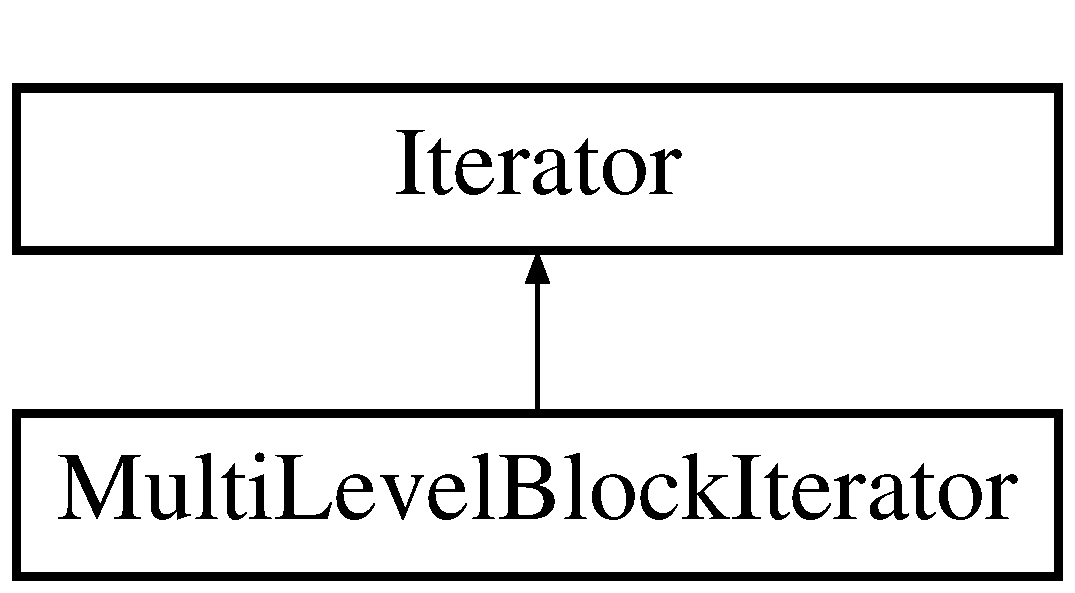
\includegraphics[height=2cm]{classIterator}
\end{center}
\end{figure}
\subsection*{Public Member Functions}
\begin{DoxyCompactItemize}
\item 
\hyperlink{classIterator_a30f4489aebb0ea1a56da6925d03eecfb}{Iterator} ()
\item 
\hyperlink{classIterator_a74d2719764b4adbc85d62efd8b7aefaf}{Iterator} (\hyperlink{classTopology}{Topology} \&topo)
\item 
\hyperlink{classIterator_aab6716f5bdecb49e9cdd754359408ab6}{$\sim$Iterator} ()
\item 
void \hyperlink{classIterator_ad08f622629417fb8913d18d95150d8de}{reformInnerTopology} ()
\item 
map$<$ \hyperlink{swMacro_8h_a113cf5f6b5377cdf3fac6aa4e443e9aa}{swInt}, \hyperlink{swMacro_8h_a113cf5f6b5377cdf3fac6aa4e443e9aa}{swInt} $>$ \& \hyperlink{classIterator_ac3a2a5c322b527888c8689dd688f9aed}{getEdgeMap} ()
\item 
map$<$ \hyperlink{swMacro_8h_a113cf5f6b5377cdf3fac6aa4e443e9aa}{swInt}, \hyperlink{swMacro_8h_a113cf5f6b5377cdf3fac6aa4e443e9aa}{swInt} $>$ \& \hyperlink{classIterator_aa40b90d401685840ead9626e4ce067f0}{getVertexMap} ()
\item 
virtual void \hyperlink{classIterator_ad467453135759642e4e4a9f9e5233771}{reorderEdgesFromEdge} (\hyperlink{swMacro_8h_a113cf5f6b5377cdf3fac6aa4e443e9aa}{swInt} $\ast$startVertices, \hyperlink{swMacro_8h_a113cf5f6b5377cdf3fac6aa4e443e9aa}{swInt} $\ast$endVertices, \hyperlink{swMacro_8h_a113cf5f6b5377cdf3fac6aa4e443e9aa}{swInt} edgeNumber, \hyperlink{swMacro_8h_a113cf5f6b5377cdf3fac6aa4e443e9aa}{swInt} vertexNumber)=0
\item 
virtual void \hyperlink{classIterator_a852bc84ccdfc84a9f0802ee070dd4cac}{reorderEdgesFromVertex} (\hyperlink{swMacro_8h_a113cf5f6b5377cdf3fac6aa4e443e9aa}{swInt} $\ast$firstEdgeVertices, \hyperlink{swMacro_8h_a113cf5f6b5377cdf3fac6aa4e443e9aa}{swInt} $\ast$vertexNeighbours, \hyperlink{swMacro_8h_a113cf5f6b5377cdf3fac6aa4e443e9aa}{swInt} edgeNumber, \hyperlink{swMacro_8h_a113cf5f6b5377cdf3fac6aa4e443e9aa}{swInt} vertexNumber)=0
\item 
virtual void \hyperlink{classIterator_a4a803a634065aba90c6a7572542aa8c3}{reorderEdgeData} (\hyperlink{structArrays}{Arrays} $\ast$edgeData)=0
\item 
virtual void \hyperlink{classIterator_aea73c3b4ba7c3cb6c56df6c5ddbe1f31}{reorderEdgeDataUnsymm} (\hyperlink{structArrays}{Arrays} $\ast$edgeData)=0
\item 
virtual void \hyperlink{classIterator_abe5bcf1a342b1ed4e3a5efe7f630e6d9}{reorderVertexData} (\hyperlink{structArrays}{Arrays} $\ast$edgeData)=0
\item 
virtual void \hyperlink{classIterator_a9606486fd118ee0131bc85a4c825feb8}{edge2VertexIteration} (\hyperlink{structArrays}{Arrays} $\ast$edgeData, \hyperlink{structArrays}{Arrays} $\ast$vertexData, void($\ast$\hyperlink{test_8cpp_aecc50c51899b7a8153dc83e95c3e6976}{operatorFunPointer\_\-host})(\hyperlink{structMLBFunParameters}{MLBFunParameters} $\ast$MLBFunParas), void($\ast$\hyperlink{test_8cpp_a434737e1969edf175d1bea960d600584}{operatorFunPointer\_\-slave})(\hyperlink{structMLBFunParameters}{MLBFunParameters} $\ast$MLBFunParas))=0
\item 
virtual void \hyperlink{classIterator_af3f4a8ad925b4a2029d9b2db74787094}{vertex2EdgeIteration} (\hyperlink{structArrays}{Arrays} $\ast$neighbourData, \hyperlink{structArrays}{Arrays} $\ast$vertexData, void($\ast$\hyperlink{test_8cpp_aecc50c51899b7a8153dc83e95c3e6976}{operatorFunPointer\_\-host})(\hyperlink{structMLBFunParameters}{MLBFunParameters} $\ast$MLBFunParas), void($\ast$\hyperlink{test_8cpp_a434737e1969edf175d1bea960d600584}{operatorFunPointer\_\-slave})(\hyperlink{structMLBFunParameters}{MLBFunParameters} $\ast$MLBFunParas))=0
\end{DoxyCompactItemize}
\subsection*{Protected Member Functions}
\begin{DoxyCompactItemize}
\item 
\hyperlink{classTopology}{Topology} $\ast$ \hyperlink{classIterator_a1fd2f17fcb324b5f3c31c42f65185ba9}{getTopology} ()
\end{DoxyCompactItemize}
\subsection*{Private Attributes}
\begin{DoxyCompactItemize}
\item 
\hyperlink{classTopology}{Topology} $\ast$ \hyperlink{classIterator_a8c90147f6541ebb64ae6fb68d622a2fb}{\_\-topo}
\item 
map$<$ \hyperlink{swMacro_8h_a113cf5f6b5377cdf3fac6aa4e443e9aa}{swInt}, \hyperlink{swMacro_8h_a113cf5f6b5377cdf3fac6aa4e443e9aa}{swInt} $>$ \hyperlink{classIterator_aedde11e435ff2559186706fdbbd3fe5a}{\_\-edgeMap}
\item 
map$<$ \hyperlink{swMacro_8h_a113cf5f6b5377cdf3fac6aa4e443e9aa}{swInt}, \hyperlink{swMacro_8h_a113cf5f6b5377cdf3fac6aa4e443e9aa}{swInt} $>$ \hyperlink{classIterator_a3c329666d26e1f9d74a61b46adcadd74}{\_\-vertexMap}
\end{DoxyCompactItemize}


\subsection{Constructor \& Destructor Documentation}
\hypertarget{classIterator_a30f4489aebb0ea1a56da6925d03eecfb}{
\index{Iterator@{Iterator}!Iterator@{Iterator}}
\index{Iterator@{Iterator}!Iterator@{Iterator}}
\subsubsection[{Iterator}]{\setlength{\rightskip}{0pt plus 5cm}Iterator::Iterator ()\hspace{0.3cm}{\ttfamily  \mbox{[}inline\mbox{]}}}}
\label{classIterator_a30f4489aebb0ea1a56da6925d03eecfb}
\hypertarget{classIterator_a74d2719764b4adbc85d62efd8b7aefaf}{
\index{Iterator@{Iterator}!Iterator@{Iterator}}
\index{Iterator@{Iterator}!Iterator@{Iterator}}
\subsubsection[{Iterator}]{\setlength{\rightskip}{0pt plus 5cm}Iterator::Iterator ({\bf Topology} \& {\em topo})\hspace{0.3cm}{\ttfamily  \mbox{[}inline\mbox{]}}}}
\label{classIterator_a74d2719764b4adbc85d62efd8b7aefaf}
\hypertarget{classIterator_aab6716f5bdecb49e9cdd754359408ab6}{
\index{Iterator@{Iterator}!$\sim$Iterator@{$\sim$Iterator}}
\index{$\sim$Iterator@{$\sim$Iterator}!Iterator@{Iterator}}
\subsubsection[{$\sim$Iterator}]{\setlength{\rightskip}{0pt plus 5cm}Iterator::$\sim$Iterator ()\hspace{0.3cm}{\ttfamily  \mbox{[}inline\mbox{]}}}}
\label{classIterator_aab6716f5bdecb49e9cdd754359408ab6}


\subsection{Member Function Documentation}
\hypertarget{classIterator_a9606486fd118ee0131bc85a4c825feb8}{
\index{Iterator@{Iterator}!edge2VertexIteration@{edge2VertexIteration}}
\index{edge2VertexIteration@{edge2VertexIteration}!Iterator@{Iterator}}
\subsubsection[{edge2VertexIteration}]{\setlength{\rightskip}{0pt plus 5cm}virtual void Iterator::edge2VertexIteration ({\bf Arrays} $\ast$ {\em edgeData}, \/  {\bf Arrays} $\ast$ {\em vertexData}, \/  void($\ast$)({\bf MLBFunParameters} $\ast$MLBFunParas) {\em operatorFunPointer\_\-host}, \/  void($\ast$)({\bf MLBFunParameters} $\ast$MLBFunParas) {\em operatorFunPointer\_\-slave})\hspace{0.3cm}{\ttfamily  \mbox{[}pure virtual\mbox{]}}}}
\label{classIterator_a9606486fd118ee0131bc85a4c825feb8}


Implemented in \hyperlink{classMultiLevelBlockIterator_ac43a134b15498ad6e7eec873b2f45f79}{MultiLevelBlockIterator}.\hypertarget{classIterator_ac3a2a5c322b527888c8689dd688f9aed}{
\index{Iterator@{Iterator}!getEdgeMap@{getEdgeMap}}
\index{getEdgeMap@{getEdgeMap}!Iterator@{Iterator}}
\subsubsection[{getEdgeMap}]{\setlength{\rightskip}{0pt plus 5cm}map$<${\bf swInt}, {\bf swInt}$>$\& Iterator::getEdgeMap ()\hspace{0.3cm}{\ttfamily  \mbox{[}inline\mbox{]}}}}
\label{classIterator_ac3a2a5c322b527888c8689dd688f9aed}
\hypertarget{classIterator_a1fd2f17fcb324b5f3c31c42f65185ba9}{
\index{Iterator@{Iterator}!getTopology@{getTopology}}
\index{getTopology@{getTopology}!Iterator@{Iterator}}
\subsubsection[{getTopology}]{\setlength{\rightskip}{0pt plus 5cm}{\bf Topology}$\ast$ Iterator::getTopology ()\hspace{0.3cm}{\ttfamily  \mbox{[}inline, protected\mbox{]}}}}
\label{classIterator_a1fd2f17fcb324b5f3c31c42f65185ba9}
\hypertarget{classIterator_aa40b90d401685840ead9626e4ce067f0}{
\index{Iterator@{Iterator}!getVertexMap@{getVertexMap}}
\index{getVertexMap@{getVertexMap}!Iterator@{Iterator}}
\subsubsection[{getVertexMap}]{\setlength{\rightskip}{0pt plus 5cm}map$<${\bf swInt}, {\bf swInt}$>$\& Iterator::getVertexMap ()\hspace{0.3cm}{\ttfamily  \mbox{[}inline\mbox{]}}}}
\label{classIterator_aa40b90d401685840ead9626e4ce067f0}
\hypertarget{classIterator_ad08f622629417fb8913d18d95150d8de}{
\index{Iterator@{Iterator}!reformInnerTopology@{reformInnerTopology}}
\index{reformInnerTopology@{reformInnerTopology}!Iterator@{Iterator}}
\subsubsection[{reformInnerTopology}]{\setlength{\rightskip}{0pt plus 5cm}void Iterator::reformInnerTopology ()\hspace{0.3cm}{\ttfamily  \mbox{[}inline\mbox{]}}}}
\label{classIterator_ad08f622629417fb8913d18d95150d8de}
\hypertarget{classIterator_a4a803a634065aba90c6a7572542aa8c3}{
\index{Iterator@{Iterator}!reorderEdgeData@{reorderEdgeData}}
\index{reorderEdgeData@{reorderEdgeData}!Iterator@{Iterator}}
\subsubsection[{reorderEdgeData}]{\setlength{\rightskip}{0pt plus 5cm}virtual void Iterator::reorderEdgeData ({\bf Arrays} $\ast$ {\em edgeData})\hspace{0.3cm}{\ttfamily  \mbox{[}pure virtual\mbox{]}}}}
\label{classIterator_a4a803a634065aba90c6a7572542aa8c3}


Implemented in \hyperlink{classMultiLevelBlockIterator_a6db1df64cc6cb8c7fdc8ad6587f51a87}{MultiLevelBlockIterator}.\hypertarget{classIterator_aea73c3b4ba7c3cb6c56df6c5ddbe1f31}{
\index{Iterator@{Iterator}!reorderEdgeDataUnsymm@{reorderEdgeDataUnsymm}}
\index{reorderEdgeDataUnsymm@{reorderEdgeDataUnsymm}!Iterator@{Iterator}}
\subsubsection[{reorderEdgeDataUnsymm}]{\setlength{\rightskip}{0pt plus 5cm}virtual void Iterator::reorderEdgeDataUnsymm ({\bf Arrays} $\ast$ {\em edgeData})\hspace{0.3cm}{\ttfamily  \mbox{[}pure virtual\mbox{]}}}}
\label{classIterator_aea73c3b4ba7c3cb6c56df6c5ddbe1f31}


Implemented in \hyperlink{classMultiLevelBlockIterator_a96adad6f8220ff77653f75150bbd1b3c}{MultiLevelBlockIterator}.\hypertarget{classIterator_ad467453135759642e4e4a9f9e5233771}{
\index{Iterator@{Iterator}!reorderEdgesFromEdge@{reorderEdgesFromEdge}}
\index{reorderEdgesFromEdge@{reorderEdgesFromEdge}!Iterator@{Iterator}}
\subsubsection[{reorderEdgesFromEdge}]{\setlength{\rightskip}{0pt plus 5cm}virtual void Iterator::reorderEdgesFromEdge ({\bf swInt} $\ast$ {\em startVertices}, \/  {\bf swInt} $\ast$ {\em endVertices}, \/  {\bf swInt} {\em edgeNumber}, \/  {\bf swInt} {\em vertexNumber})\hspace{0.3cm}{\ttfamily  \mbox{[}pure virtual\mbox{]}}}}
\label{classIterator_ad467453135759642e4e4a9f9e5233771}


Implemented in \hyperlink{classMultiLevelBlockIterator_a329b89b35011569fd4c4c3e93518eea3}{MultiLevelBlockIterator}.\hypertarget{classIterator_a852bc84ccdfc84a9f0802ee070dd4cac}{
\index{Iterator@{Iterator}!reorderEdgesFromVertex@{reorderEdgesFromVertex}}
\index{reorderEdgesFromVertex@{reorderEdgesFromVertex}!Iterator@{Iterator}}
\subsubsection[{reorderEdgesFromVertex}]{\setlength{\rightskip}{0pt plus 5cm}virtual void Iterator::reorderEdgesFromVertex ({\bf swInt} $\ast$ {\em firstEdgeVertices}, \/  {\bf swInt} $\ast$ {\em vertexNeighbours}, \/  {\bf swInt} {\em edgeNumber}, \/  {\bf swInt} {\em vertexNumber})\hspace{0.3cm}{\ttfamily  \mbox{[}pure virtual\mbox{]}}}}
\label{classIterator_a852bc84ccdfc84a9f0802ee070dd4cac}


Implemented in \hyperlink{classMultiLevelBlockIterator_af2bc453fc11f9e0ba34a1edc7eafc34e}{MultiLevelBlockIterator}.\hypertarget{classIterator_abe5bcf1a342b1ed4e3a5efe7f630e6d9}{
\index{Iterator@{Iterator}!reorderVertexData@{reorderVertexData}}
\index{reorderVertexData@{reorderVertexData}!Iterator@{Iterator}}
\subsubsection[{reorderVertexData}]{\setlength{\rightskip}{0pt plus 5cm}virtual void Iterator::reorderVertexData ({\bf Arrays} $\ast$ {\em edgeData})\hspace{0.3cm}{\ttfamily  \mbox{[}pure virtual\mbox{]}}}}
\label{classIterator_abe5bcf1a342b1ed4e3a5efe7f630e6d9}


Implemented in \hyperlink{classMultiLevelBlockIterator_ac442935a4731bb5ae8548bad040ac692}{MultiLevelBlockIterator}.\hypertarget{classIterator_af3f4a8ad925b4a2029d9b2db74787094}{
\index{Iterator@{Iterator}!vertex2EdgeIteration@{vertex2EdgeIteration}}
\index{vertex2EdgeIteration@{vertex2EdgeIteration}!Iterator@{Iterator}}
\subsubsection[{vertex2EdgeIteration}]{\setlength{\rightskip}{0pt plus 5cm}virtual void Iterator::vertex2EdgeIteration ({\bf Arrays} $\ast$ {\em neighbourData}, \/  {\bf Arrays} $\ast$ {\em vertexData}, \/  void($\ast$)({\bf MLBFunParameters} $\ast$MLBFunParas) {\em operatorFunPointer\_\-host}, \/  void($\ast$)({\bf MLBFunParameters} $\ast$MLBFunParas) {\em operatorFunPointer\_\-slave})\hspace{0.3cm}{\ttfamily  \mbox{[}pure virtual\mbox{]}}}}
\label{classIterator_af3f4a8ad925b4a2029d9b2db74787094}


Implemented in \hyperlink{classMultiLevelBlockIterator_ac4035c51b1a940a7661a7e1b15e7b086}{MultiLevelBlockIterator}.

\subsection{Member Data Documentation}
\hypertarget{classIterator_aedde11e435ff2559186706fdbbd3fe5a}{
\index{Iterator@{Iterator}!\_\-edgeMap@{\_\-edgeMap}}
\index{\_\-edgeMap@{\_\-edgeMap}!Iterator@{Iterator}}
\subsubsection[{\_\-edgeMap}]{\setlength{\rightskip}{0pt plus 5cm}map$<${\bf swInt}, {\bf swInt}$>$ {\bf Iterator::\_\-edgeMap}\hspace{0.3cm}{\ttfamily  \mbox{[}private\mbox{]}}}}
\label{classIterator_aedde11e435ff2559186706fdbbd3fe5a}
\hypertarget{classIterator_a8c90147f6541ebb64ae6fb68d622a2fb}{
\index{Iterator@{Iterator}!\_\-topo@{\_\-topo}}
\index{\_\-topo@{\_\-topo}!Iterator@{Iterator}}
\subsubsection[{\_\-topo}]{\setlength{\rightskip}{0pt plus 5cm}{\bf Topology}$\ast$ {\bf Iterator::\_\-topo}\hspace{0.3cm}{\ttfamily  \mbox{[}private\mbox{]}}}}
\label{classIterator_a8c90147f6541ebb64ae6fb68d622a2fb}
\hypertarget{classIterator_a3c329666d26e1f9d74a61b46adcadd74}{
\index{Iterator@{Iterator}!\_\-vertexMap@{\_\-vertexMap}}
\index{\_\-vertexMap@{\_\-vertexMap}!Iterator@{Iterator}}
\subsubsection[{\_\-vertexMap}]{\setlength{\rightskip}{0pt plus 5cm}map$<${\bf swInt}, {\bf swInt}$>$ {\bf Iterator::\_\-vertexMap}\hspace{0.3cm}{\ttfamily  \mbox{[}private\mbox{]}}}}
\label{classIterator_a3c329666d26e1f9d74a61b46adcadd74}


The documentation for this class was generated from the following file:\begin{DoxyCompactItemize}
\item 
iterator/\hyperlink{iterator_8H}{iterator.H}\end{DoxyCompactItemize}

\hypertarget{structMLBFunParameters}{
\section{MLBFunParameters Struct Reference}
\label{structMLBFunParameters}\index{MLBFunParameters@{MLBFunParameters}}
}


{\ttfamily \#include $<$iterator\_\-struct.h$>$}\subsection*{Public Attributes}
\begin{DoxyCompactItemize}
\item 
\hyperlink{structArrays}{Arrays} $\ast$ \hyperlink{structMLBFunParameters_a877290c3746a4a1443e312d225dc6963}{edgeData}
\item 
\hyperlink{structArrays}{Arrays} $\ast$ \hyperlink{structMLBFunParameters_ac10ea14c3141f3e566dee0568f1f4b2f}{vertexData}
\item 
\hyperlink{structtopoArrays}{topoArrays} $\ast$ \hyperlink{structMLBFunParameters_ae7e20a4db032dafb9a56836cfb3a4ea8}{tArrays}
\item 
\hyperlink{swMacro_8h_a113cf5f6b5377cdf3fac6aa4e443e9aa}{swInt} \hyperlink{structMLBFunParameters_a3bde90af55aad6097d41a322c89f3578}{count}
\item 
\hyperlink{swMacro_8h_a113cf5f6b5377cdf3fac6aa4e443e9aa}{swInt} \hyperlink{structMLBFunParameters_acc4e1b0ab4700da0f0a68a617209aebb}{k1}
\item 
\hyperlink{swMacro_8h_a113cf5f6b5377cdf3fac6aa4e443e9aa}{swInt} \hyperlink{structMLBFunParameters_ae30f1ae18cf7dc38b28d8dcacfe57eff}{k2}
\item 
\hyperlink{swMacro_8h_a113cf5f6b5377cdf3fac6aa4e443e9aa}{swInt} \hyperlink{structMLBFunParameters_a7e2c8948155a41ba59c48aa27e78c50a}{flag}
\end{DoxyCompactItemize}


\subsection{Member Data Documentation}
\hypertarget{structMLBFunParameters_a3bde90af55aad6097d41a322c89f3578}{
\index{MLBFunParameters@{MLBFunParameters}!count@{count}}
\index{count@{count}!MLBFunParameters@{MLBFunParameters}}
\subsubsection[{count}]{\setlength{\rightskip}{0pt plus 5cm}{\bf swInt} {\bf MLBFunParameters::count}}}
\label{structMLBFunParameters_a3bde90af55aad6097d41a322c89f3578}
\hypertarget{structMLBFunParameters_a877290c3746a4a1443e312d225dc6963}{
\index{MLBFunParameters@{MLBFunParameters}!edgeData@{edgeData}}
\index{edgeData@{edgeData}!MLBFunParameters@{MLBFunParameters}}
\subsubsection[{edgeData}]{\setlength{\rightskip}{0pt plus 5cm}{\bf Arrays}$\ast$ {\bf MLBFunParameters::edgeData}}}
\label{structMLBFunParameters_a877290c3746a4a1443e312d225dc6963}
\hypertarget{structMLBFunParameters_a7e2c8948155a41ba59c48aa27e78c50a}{
\index{MLBFunParameters@{MLBFunParameters}!flag@{flag}}
\index{flag@{flag}!MLBFunParameters@{MLBFunParameters}}
\subsubsection[{flag}]{\setlength{\rightskip}{0pt plus 5cm}{\bf swInt} {\bf MLBFunParameters::flag}}}
\label{structMLBFunParameters_a7e2c8948155a41ba59c48aa27e78c50a}
\hypertarget{structMLBFunParameters_acc4e1b0ab4700da0f0a68a617209aebb}{
\index{MLBFunParameters@{MLBFunParameters}!k1@{k1}}
\index{k1@{k1}!MLBFunParameters@{MLBFunParameters}}
\subsubsection[{k1}]{\setlength{\rightskip}{0pt plus 5cm}{\bf swInt} {\bf MLBFunParameters::k1}}}
\label{structMLBFunParameters_acc4e1b0ab4700da0f0a68a617209aebb}
\hypertarget{structMLBFunParameters_ae30f1ae18cf7dc38b28d8dcacfe57eff}{
\index{MLBFunParameters@{MLBFunParameters}!k2@{k2}}
\index{k2@{k2}!MLBFunParameters@{MLBFunParameters}}
\subsubsection[{k2}]{\setlength{\rightskip}{0pt plus 5cm}{\bf swInt} {\bf MLBFunParameters::k2}}}
\label{structMLBFunParameters_ae30f1ae18cf7dc38b28d8dcacfe57eff}
\hypertarget{structMLBFunParameters_ae7e20a4db032dafb9a56836cfb3a4ea8}{
\index{MLBFunParameters@{MLBFunParameters}!tArrays@{tArrays}}
\index{tArrays@{tArrays}!MLBFunParameters@{MLBFunParameters}}
\subsubsection[{tArrays}]{\setlength{\rightskip}{0pt plus 5cm}{\bf topoArrays}$\ast$ {\bf MLBFunParameters::tArrays}}}
\label{structMLBFunParameters_ae7e20a4db032dafb9a56836cfb3a4ea8}
\hypertarget{structMLBFunParameters_ac10ea14c3141f3e566dee0568f1f4b2f}{
\index{MLBFunParameters@{MLBFunParameters}!vertexData@{vertexData}}
\index{vertexData@{vertexData}!MLBFunParameters@{MLBFunParameters}}
\subsubsection[{vertexData}]{\setlength{\rightskip}{0pt plus 5cm}{\bf Arrays}$\ast$ {\bf MLBFunParameters::vertexData}}}
\label{structMLBFunParameters_ac10ea14c3141f3e566dee0568f1f4b2f}


The documentation for this struct was generated from the following file:\begin{DoxyCompactItemize}
\item 
iterator/\hyperlink{iterator__struct_8h}{iterator\_\-struct.h}\end{DoxyCompactItemize}

\hypertarget{structMLBParameters}{
\section{MLBParameters Struct Reference}
\label{structMLBParameters}\index{MLBParameters@{MLBParameters}}
}


{\ttfamily \#include $<$iterator\_\-struct.h$>$}\subsection*{Public Attributes}
\begin{DoxyCompactItemize}
\item 
\hyperlink{swMacro_8h_a113cf5f6b5377cdf3fac6aa4e443e9aa}{swInt} $\ast$ \hyperlink{structMLBParameters_af9b86ffe9fdb9d60b4b4adb2983c60d6}{blockStarts}
\item 
\hyperlink{swMacro_8h_a113cf5f6b5377cdf3fac6aa4e443e9aa}{swInt} $\ast$ \hyperlink{structMLBParameters_a0de1bb277dcff80762fd752f77ec75b9}{blockStartsUnsymm}
\item 
\hyperlink{swMacro_8h_a113cf5f6b5377cdf3fac6aa4e443e9aa}{swInt} $\ast$ \hyperlink{structMLBParameters_aba1b1654ae819032fd78dac4febe0101}{vertexStarts}
\item 
\hyperlink{swMacro_8h_a113cf5f6b5377cdf3fac6aa4e443e9aa}{swInt} $\ast$ \hyperlink{structMLBParameters_ac7483bc6365005100466360bb542fc31}{owner}
\item 
\hyperlink{swMacro_8h_a113cf5f6b5377cdf3fac6aa4e443e9aa}{swInt} $\ast$ \hyperlink{structMLBParameters_a2f37a3f6bfcd23b1f2e57c613325484d}{neighbor}
\item 
\hyperlink{swMacro_8h_a113cf5f6b5377cdf3fac6aa4e443e9aa}{swInt} $\ast$ \hyperlink{structMLBParameters_aef7de09684f1521d2b1eeacfcd2b6d0d}{firstEdgeVertices}
\item 
\hyperlink{swMacro_8h_a113cf5f6b5377cdf3fac6aa4e443e9aa}{swInt} $\ast$ \hyperlink{structMLBParameters_aed04421df60bb1fa6144f4f8b03b789a}{vertexNeighbor}
\item 
\hyperlink{swMacro_8h_a113cf5f6b5377cdf3fac6aa4e443e9aa}{swInt} \hyperlink{structMLBParameters_ad5c2db1dad6930b3786e050d0f52c436}{cpeBlockNum}
\item 
\hyperlink{swMacro_8h_a113cf5f6b5377cdf3fac6aa4e443e9aa}{swInt} \hyperlink{structMLBParameters_ad276c2308b307b00101575ba6df0cb76}{mshBlockNum}
\item 
\hyperlink{swMacro_8h_a113cf5f6b5377cdf3fac6aa4e443e9aa}{swInt} \hyperlink{structMLBParameters_a110a1c5cb8f84d662e0de090422104fa}{mtxBlockNum}
\item 
\hyperlink{swMacro_8h_a113cf5f6b5377cdf3fac6aa4e443e9aa}{swInt} \hyperlink{structMLBParameters_a2d2166d1e3bd56f2265645cc826996dc}{maxXNum}
\item 
\hyperlink{swMacro_8h_a113cf5f6b5377cdf3fac6aa4e443e9aa}{swInt} \hyperlink{structMLBParameters_aace8685526e0a7bc2da72db8e6f9b02c}{maxCells}
\item 
\hyperlink{swMacro_8h_a113cf5f6b5377cdf3fac6aa4e443e9aa}{swInt} \hyperlink{structMLBParameters_ad053997c6c3dfbcb0b342e7a2b2c892e}{maxEdges}
\item 
void($\ast$ \hyperlink{structMLBParameters_ad7a8768b3710ff857ab156bf24db6548}{operatorFunPointer\_\-host} )(\hyperlink{structMLBFunParameters}{MLBFunParameters} $\ast$MLBFunParas)
\item 
void($\ast$ \hyperlink{structMLBParameters_aec73e8d9f7b561d3a80658ee8a3eb397}{operatorFunPointer\_\-slave} )(\hyperlink{structMLBFunParameters}{MLBFunParameters} $\ast$MLBFunParas)
\end{DoxyCompactItemize}


\subsection{Member Data Documentation}
\hypertarget{structMLBParameters_af9b86ffe9fdb9d60b4b4adb2983c60d6}{
\index{MLBParameters@{MLBParameters}!blockStarts@{blockStarts}}
\index{blockStarts@{blockStarts}!MLBParameters@{MLBParameters}}
\subsubsection[{blockStarts}]{\setlength{\rightskip}{0pt plus 5cm}{\bf swInt}$\ast$ {\bf MLBParameters::blockStarts}}}
\label{structMLBParameters_af9b86ffe9fdb9d60b4b4adb2983c60d6}
\hypertarget{structMLBParameters_a0de1bb277dcff80762fd752f77ec75b9}{
\index{MLBParameters@{MLBParameters}!blockStartsUnsymm@{blockStartsUnsymm}}
\index{blockStartsUnsymm@{blockStartsUnsymm}!MLBParameters@{MLBParameters}}
\subsubsection[{blockStartsUnsymm}]{\setlength{\rightskip}{0pt plus 5cm}{\bf swInt}$\ast$ {\bf MLBParameters::blockStartsUnsymm}}}
\label{structMLBParameters_a0de1bb277dcff80762fd752f77ec75b9}
\hypertarget{structMLBParameters_ad5c2db1dad6930b3786e050d0f52c436}{
\index{MLBParameters@{MLBParameters}!cpeBlockNum@{cpeBlockNum}}
\index{cpeBlockNum@{cpeBlockNum}!MLBParameters@{MLBParameters}}
\subsubsection[{cpeBlockNum}]{\setlength{\rightskip}{0pt plus 5cm}{\bf swInt} {\bf MLBParameters::cpeBlockNum}}}
\label{structMLBParameters_ad5c2db1dad6930b3786e050d0f52c436}
\hypertarget{structMLBParameters_aef7de09684f1521d2b1eeacfcd2b6d0d}{
\index{MLBParameters@{MLBParameters}!firstEdgeVertices@{firstEdgeVertices}}
\index{firstEdgeVertices@{firstEdgeVertices}!MLBParameters@{MLBParameters}}
\subsubsection[{firstEdgeVertices}]{\setlength{\rightskip}{0pt plus 5cm}{\bf swInt}$\ast$ {\bf MLBParameters::firstEdgeVertices}}}
\label{structMLBParameters_aef7de09684f1521d2b1eeacfcd2b6d0d}
\hypertarget{structMLBParameters_aace8685526e0a7bc2da72db8e6f9b02c}{
\index{MLBParameters@{MLBParameters}!maxCells@{maxCells}}
\index{maxCells@{maxCells}!MLBParameters@{MLBParameters}}
\subsubsection[{maxCells}]{\setlength{\rightskip}{0pt plus 5cm}{\bf swInt} {\bf MLBParameters::maxCells}}}
\label{structMLBParameters_aace8685526e0a7bc2da72db8e6f9b02c}
\hypertarget{structMLBParameters_ad053997c6c3dfbcb0b342e7a2b2c892e}{
\index{MLBParameters@{MLBParameters}!maxEdges@{maxEdges}}
\index{maxEdges@{maxEdges}!MLBParameters@{MLBParameters}}
\subsubsection[{maxEdges}]{\setlength{\rightskip}{0pt plus 5cm}{\bf swInt} {\bf MLBParameters::maxEdges}}}
\label{structMLBParameters_ad053997c6c3dfbcb0b342e7a2b2c892e}
\hypertarget{structMLBParameters_a2d2166d1e3bd56f2265645cc826996dc}{
\index{MLBParameters@{MLBParameters}!maxXNum@{maxXNum}}
\index{maxXNum@{maxXNum}!MLBParameters@{MLBParameters}}
\subsubsection[{maxXNum}]{\setlength{\rightskip}{0pt plus 5cm}{\bf swInt} {\bf MLBParameters::maxXNum}}}
\label{structMLBParameters_a2d2166d1e3bd56f2265645cc826996dc}
\hypertarget{structMLBParameters_ad276c2308b307b00101575ba6df0cb76}{
\index{MLBParameters@{MLBParameters}!mshBlockNum@{mshBlockNum}}
\index{mshBlockNum@{mshBlockNum}!MLBParameters@{MLBParameters}}
\subsubsection[{mshBlockNum}]{\setlength{\rightskip}{0pt plus 5cm}{\bf swInt} {\bf MLBParameters::mshBlockNum}}}
\label{structMLBParameters_ad276c2308b307b00101575ba6df0cb76}
\hypertarget{structMLBParameters_a110a1c5cb8f84d662e0de090422104fa}{
\index{MLBParameters@{MLBParameters}!mtxBlockNum@{mtxBlockNum}}
\index{mtxBlockNum@{mtxBlockNum}!MLBParameters@{MLBParameters}}
\subsubsection[{mtxBlockNum}]{\setlength{\rightskip}{0pt plus 5cm}{\bf swInt} {\bf MLBParameters::mtxBlockNum}}}
\label{structMLBParameters_a110a1c5cb8f84d662e0de090422104fa}
\hypertarget{structMLBParameters_a2f37a3f6bfcd23b1f2e57c613325484d}{
\index{MLBParameters@{MLBParameters}!neighbor@{neighbor}}
\index{neighbor@{neighbor}!MLBParameters@{MLBParameters}}
\subsubsection[{neighbor}]{\setlength{\rightskip}{0pt plus 5cm}{\bf swInt}$\ast$ {\bf MLBParameters::neighbor}}}
\label{structMLBParameters_a2f37a3f6bfcd23b1f2e57c613325484d}
\hypertarget{structMLBParameters_ad7a8768b3710ff857ab156bf24db6548}{
\index{MLBParameters@{MLBParameters}!operatorFunPointer\_\-host@{operatorFunPointer\_\-host}}
\index{operatorFunPointer\_\-host@{operatorFunPointer\_\-host}!MLBParameters@{MLBParameters}}
\subsubsection[{operatorFunPointer\_\-host}]{\setlength{\rightskip}{0pt plus 5cm}void($\ast$ {\bf MLBParameters::operatorFunPointer\_\-host})({\bf MLBFunParameters} $\ast$MLBFunParas)}}
\label{structMLBParameters_ad7a8768b3710ff857ab156bf24db6548}
\hypertarget{structMLBParameters_aec73e8d9f7b561d3a80658ee8a3eb397}{
\index{MLBParameters@{MLBParameters}!operatorFunPointer\_\-slave@{operatorFunPointer\_\-slave}}
\index{operatorFunPointer\_\-slave@{operatorFunPointer\_\-slave}!MLBParameters@{MLBParameters}}
\subsubsection[{operatorFunPointer\_\-slave}]{\setlength{\rightskip}{0pt plus 5cm}void($\ast$ {\bf MLBParameters::operatorFunPointer\_\-slave})({\bf MLBFunParameters} $\ast$MLBFunParas)}}
\label{structMLBParameters_aec73e8d9f7b561d3a80658ee8a3eb397}
\hypertarget{structMLBParameters_ac7483bc6365005100466360bb542fc31}{
\index{MLBParameters@{MLBParameters}!owner@{owner}}
\index{owner@{owner}!MLBParameters@{MLBParameters}}
\subsubsection[{owner}]{\setlength{\rightskip}{0pt plus 5cm}{\bf swInt}$\ast$ {\bf MLBParameters::owner}}}
\label{structMLBParameters_ac7483bc6365005100466360bb542fc31}
\hypertarget{structMLBParameters_aed04421df60bb1fa6144f4f8b03b789a}{
\index{MLBParameters@{MLBParameters}!vertexNeighbor@{vertexNeighbor}}
\index{vertexNeighbor@{vertexNeighbor}!MLBParameters@{MLBParameters}}
\subsubsection[{vertexNeighbor}]{\setlength{\rightskip}{0pt plus 5cm}{\bf swInt}$\ast$ {\bf MLBParameters::vertexNeighbor}}}
\label{structMLBParameters_aed04421df60bb1fa6144f4f8b03b789a}
\hypertarget{structMLBParameters_aba1b1654ae819032fd78dac4febe0101}{
\index{MLBParameters@{MLBParameters}!vertexStarts@{vertexStarts}}
\index{vertexStarts@{vertexStarts}!MLBParameters@{MLBParameters}}
\subsubsection[{vertexStarts}]{\setlength{\rightskip}{0pt plus 5cm}{\bf swInt}$\ast$ {\bf MLBParameters::vertexStarts}}}
\label{structMLBParameters_aba1b1654ae819032fd78dac4febe0101}


The documentation for this struct was generated from the following file:\begin{DoxyCompactItemize}
\item 
iterator/\hyperlink{iterator__struct_8h}{iterator\_\-struct.h}\end{DoxyCompactItemize}

\hypertarget{classMultiLevelBlockIterator}{
\section{MultiLevelBlockIterator Class Reference}
\label{classMultiLevelBlockIterator}\index{MultiLevelBlockIterator@{MultiLevelBlockIterator}}
}


{\ttfamily \#include $<$multiLevelBlockIterator.H$>$}Inheritance diagram for MultiLevelBlockIterator::\begin{figure}[H]
\begin{center}
\leavevmode
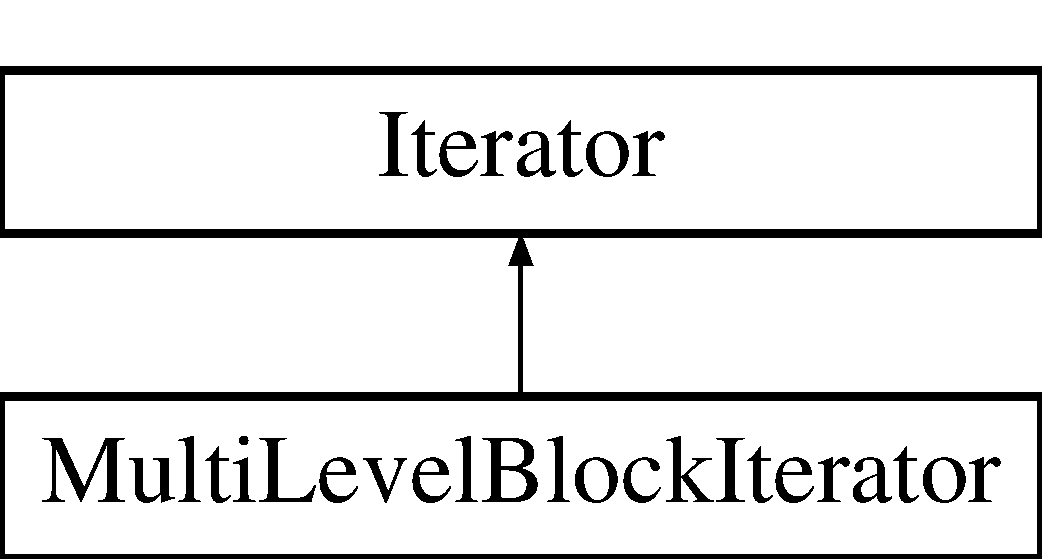
\includegraphics[height=2cm]{classMultiLevelBlockIterator}
\end{center}
\end{figure}
\subsection*{Public Member Functions}
\begin{DoxyCompactItemize}
\item 
\hyperlink{classMultiLevelBlockIterator_a6d43aae7b5472800853effe7fb4c122a}{MultiLevelBlockIterator} (\hyperlink{classTopology}{Topology} \&topo)
\item 
\hyperlink{classMultiLevelBlockIterator_ae18852417b5b2b7db13b4aa727afa106}{$\sim$MultiLevelBlockIterator} ()
\item 
void \hyperlink{classMultiLevelBlockIterator_a329b89b35011569fd4c4c3e93518eea3}{reorderEdgesFromEdge} (\hyperlink{swMacro_8h_a113cf5f6b5377cdf3fac6aa4e443e9aa}{swInt} $\ast$startVertices, \hyperlink{swMacro_8h_a113cf5f6b5377cdf3fac6aa4e443e9aa}{swInt} $\ast$endVertices, \hyperlink{swMacro_8h_a113cf5f6b5377cdf3fac6aa4e443e9aa}{swInt} edgeNumber, \hyperlink{swMacro_8h_a113cf5f6b5377cdf3fac6aa4e443e9aa}{swInt} vertexNumber)
\item 
void \hyperlink{classMultiLevelBlockIterator_af2bc453fc11f9e0ba34a1edc7eafc34e}{reorderEdgesFromVertex} (\hyperlink{swMacro_8h_a113cf5f6b5377cdf3fac6aa4e443e9aa}{swInt} $\ast$firstEdgeVertices, \hyperlink{swMacro_8h_a113cf5f6b5377cdf3fac6aa4e443e9aa}{swInt} $\ast$vertexNeighbours, \hyperlink{swMacro_8h_a113cf5f6b5377cdf3fac6aa4e443e9aa}{swInt} edgeNumber, \hyperlink{swMacro_8h_a113cf5f6b5377cdf3fac6aa4e443e9aa}{swInt} vertexNumber)
\item 
void \hyperlink{classMultiLevelBlockIterator_ac43a134b15498ad6e7eec873b2f45f79}{edge2VertexIteration} (\hyperlink{structArrays}{Arrays} $\ast$edgeData, \hyperlink{structArrays}{Arrays} $\ast$vertexData, void($\ast$\hyperlink{test_8cpp_aecc50c51899b7a8153dc83e95c3e6976}{operatorFunPointer\_\-host})(\hyperlink{structMLBFunParameters}{MLBFunParameters} $\ast$MLBFunParas), void($\ast$\hyperlink{test_8cpp_a434737e1969edf175d1bea960d600584}{operatorFunPointer\_\-slave})(\hyperlink{structMLBFunParameters}{MLBFunParameters} $\ast$MLBFunParas))
\item 
void \hyperlink{classMultiLevelBlockIterator_ac4035c51b1a940a7661a7e1b15e7b086}{vertex2EdgeIteration} (\hyperlink{structArrays}{Arrays} $\ast$neighbourData, \hyperlink{structArrays}{Arrays} $\ast$vertexData, void($\ast$\hyperlink{test_8cpp_aecc50c51899b7a8153dc83e95c3e6976}{operatorFunPointer\_\-host})(\hyperlink{structMLBFunParameters}{MLBFunParameters} $\ast$MLBFunParas), void($\ast$\hyperlink{test_8cpp_a434737e1969edf175d1bea960d600584}{operatorFunPointer\_\-slave})(\hyperlink{structMLBFunParameters}{MLBFunParameters} $\ast$MLBFunParas))
\item 
void \hyperlink{classMultiLevelBlockIterator_a6db1df64cc6cb8c7fdc8ad6587f51a87}{reorderEdgeData} (\hyperlink{structArrays}{Arrays} $\ast$edgeData)
\item 
void \hyperlink{classMultiLevelBlockIterator_a96adad6f8220ff77653f75150bbd1b3c}{reorderEdgeDataUnsymm} (\hyperlink{structArrays}{Arrays} $\ast$edgeData)
\item 
void \hyperlink{classMultiLevelBlockIterator_ac442935a4731bb5ae8548bad040ac692}{reorderVertexData} (\hyperlink{structArrays}{Arrays} $\ast$edgeData)
\item 
\hyperlink{swMacro_8h_a113cf5f6b5377cdf3fac6aa4e443e9aa}{swInt} \hyperlink{classMultiLevelBlockIterator_a66bb952127c40b44e45ec853e3ff7af6}{getCpeBlockNum} ()
\item 
\hyperlink{swMacro_8h_a113cf5f6b5377cdf3fac6aa4e443e9aa}{swInt} \hyperlink{classMultiLevelBlockIterator_a6076c2b3469188f4e1399c5c21216419}{getMshBlockNum} ()
\item 
\hyperlink{swMacro_8h_a113cf5f6b5377cdf3fac6aa4e443e9aa}{swInt} \hyperlink{classMultiLevelBlockIterator_a363f06fbb8acd59e7a8211bdc8afe3d5}{getMtxBlockNum} ()
\item 
\hyperlink{swMacro_8h_a113cf5f6b5377cdf3fac6aa4e443e9aa}{swInt} \hyperlink{classMultiLevelBlockIterator_a86ec532cd96ba3e75346f8dfd1011595}{getMaxXNum} ()
\item 
\hyperlink{swMacro_8h_a113cf5f6b5377cdf3fac6aa4e443e9aa}{swInt} \hyperlink{classMultiLevelBlockIterator_a39bd10d2154b5e429e49d9c9a2f82cff}{getMaxCells} ()
\item 
\hyperlink{swMacro_8h_a113cf5f6b5377cdf3fac6aa4e443e9aa}{swInt} \hyperlink{classMultiLevelBlockIterator_a29a4f30de98e453ff26d14d44ca97e65}{getMaxEdges} ()
\item 
\hyperlink{swMacro_8h_a113cf5f6b5377cdf3fac6aa4e443e9aa}{swInt} \hyperlink{classMultiLevelBlockIterator_a0148ef791de73511bb725a3d2f71d49b}{getMaxEdgesUnsymm} ()
\item 
\hyperlink{swMacro_8h_a113cf5f6b5377cdf3fac6aa4e443e9aa}{swInt} $\ast$ \hyperlink{classMultiLevelBlockIterator_afd32075e0f371fbcb5c9a577c11bdb7a}{getBlockStarts} ()
\item 
\hyperlink{swMacro_8h_a113cf5f6b5377cdf3fac6aa4e443e9aa}{swInt} $\ast$ \hyperlink{classMultiLevelBlockIterator_ac7c3935ce8f4a3d6f4634c85b6a2dc39}{getBlockStartsUnsymm} ()
\item 
\hyperlink{swMacro_8h_a113cf5f6b5377cdf3fac6aa4e443e9aa}{swInt} $\ast$ \hyperlink{classMultiLevelBlockIterator_aee947df3eaa77066c7d5fbc23a6e3ca4}{getVertexStarts} ()
\end{DoxyCompactItemize}
\subsection*{Private Member Functions}
\begin{DoxyCompactItemize}
\item 
void \hyperlink{classMultiLevelBlockIterator_a184e9a87ccff9f3eb2c5960434175936}{reorderVertexArray} (\hyperlink{swMacro_8h_a4ce60b1aa82e56b7372553a6a5bf2c0b}{swFloat} $\ast$array)
\item 
void \hyperlink{classMultiLevelBlockIterator_a2c8b4ee175d96866d03cf0196312a4ea}{reorderEdgeArrayUnsymm} (\hyperlink{swMacro_8h_a4ce60b1aa82e56b7372553a6a5bf2c0b}{swFloat} $\ast$array)
\item 
void \hyperlink{classMultiLevelBlockIterator_a40f5b13a4c39c42b035c7bf4b72e8edb}{MLBReorder} (\hyperlink{classTopology}{Topology} \&topo, \hyperlink{swMacro_8h_a113cf5f6b5377cdf3fac6aa4e443e9aa}{swInt} ref)
\end{DoxyCompactItemize}
\subsection*{Private Attributes}
\begin{DoxyCompactItemize}
\item 
\hyperlink{swMacro_8h_a113cf5f6b5377cdf3fac6aa4e443e9aa}{swInt} \hyperlink{classMultiLevelBlockIterator_a9c114d72d33e1c5117273a3f20d5786e}{\_\-cpeBlockNum}
\item 
\hyperlink{swMacro_8h_a113cf5f6b5377cdf3fac6aa4e443e9aa}{swInt} \hyperlink{classMultiLevelBlockIterator_a4ea166f78f24421ee5c61f19bfed316b}{\_\-mshBlockNum}
\item 
\hyperlink{swMacro_8h_a113cf5f6b5377cdf3fac6aa4e443e9aa}{swInt} \hyperlink{classMultiLevelBlockIterator_ae526c16297ad2215dc3781c154359aab}{\_\-mtxBlockNum}
\item 
\hyperlink{swMacro_8h_a113cf5f6b5377cdf3fac6aa4e443e9aa}{swInt} $\ast$ \hyperlink{classMultiLevelBlockIterator_a1b81d90682525ad806b12f851db9e9a4}{\_\-blockStarts}
\item 
\hyperlink{swMacro_8h_a113cf5f6b5377cdf3fac6aa4e443e9aa}{swInt} $\ast$ \hyperlink{classMultiLevelBlockIterator_ae42fe424b7278c9a9f117941bb2c59e0}{\_\-blockStartsUnsymm}
\item 
\hyperlink{swMacro_8h_a113cf5f6b5377cdf3fac6aa4e443e9aa}{swInt} $\ast$ \hyperlink{classMultiLevelBlockIterator_a89e43d3ad8cde9c322089090fa1a2413}{\_\-vertexStarts}
\item 
\hyperlink{swMacro_8h_a113cf5f6b5377cdf3fac6aa4e443e9aa}{swInt} \hyperlink{classMultiLevelBlockIterator_a44407268a1f8292caf90e7f963f601f7}{\_\-maxXNum}
\item 
\hyperlink{swMacro_8h_a113cf5f6b5377cdf3fac6aa4e443e9aa}{swInt} \hyperlink{classMultiLevelBlockIterator_ae35d89b26c36bdead2af0d18b5f614bc}{\_\-maxCells}
\item 
\hyperlink{swMacro_8h_a113cf5f6b5377cdf3fac6aa4e443e9aa}{swInt} \hyperlink{classMultiLevelBlockIterator_a01700d9c19041caee23d3de1600a3efa}{\_\-maxEdges}
\item 
\hyperlink{swMacro_8h_a113cf5f6b5377cdf3fac6aa4e443e9aa}{swInt} \hyperlink{classMultiLevelBlockIterator_a6e5c377723068f37e62d6ca0f2e7e3ee}{\_\-maxEdgesUnsymm}
\item 
\hyperlink{swMacro_8h_a113cf5f6b5377cdf3fac6aa4e443e9aa}{swInt} $\ast$ \hyperlink{classMultiLevelBlockIterator_a4054111d27eef080343d7b199cf319e7}{\_\-owner}
\item 
\hyperlink{swMacro_8h_a113cf5f6b5377cdf3fac6aa4e443e9aa}{swInt} $\ast$ \hyperlink{classMultiLevelBlockIterator_a346749a01a887ef338a94c794f577ffe}{\_\-neighbor}
\item 
\hyperlink{swMacro_8h_a113cf5f6b5377cdf3fac6aa4e443e9aa}{swInt} $\ast$ \hyperlink{classMultiLevelBlockIterator_a72ac8d61d98eb9ab3e95db11e8eb4592}{\_\-postEdgeOrder}
\item 
\hyperlink{swMacro_8h_a113cf5f6b5377cdf3fac6aa4e443e9aa}{swInt} $\ast$ \hyperlink{classMultiLevelBlockIterator_a68c79e502eb1bae881fe08b25eeea2e3}{\_\-postVertexOrder}
\item 
\hyperlink{swMacro_8h_a113cf5f6b5377cdf3fac6aa4e443e9aa}{swInt} $\ast$ \hyperlink{classMultiLevelBlockIterator_ad01e907226fdf1af73ce3bc3ef11ef46}{\_\-firstEdgeVertices}
\item 
\hyperlink{swMacro_8h_a113cf5f6b5377cdf3fac6aa4e443e9aa}{swInt} $\ast$ \hyperlink{classMultiLevelBlockIterator_a8e339eb75b0dfb8a789d9db1727b73c4}{\_\-vertexNeighbours}
\end{DoxyCompactItemize}


\subsection{Constructor \& Destructor Documentation}
\hypertarget{classMultiLevelBlockIterator_a6d43aae7b5472800853effe7fb4c122a}{
\index{MultiLevelBlockIterator@{MultiLevelBlockIterator}!MultiLevelBlockIterator@{MultiLevelBlockIterator}}
\index{MultiLevelBlockIterator@{MultiLevelBlockIterator}!MultiLevelBlockIterator@{MultiLevelBlockIterator}}
\subsubsection[{MultiLevelBlockIterator}]{\setlength{\rightskip}{0pt plus 5cm}MultiLevelBlockIterator::MultiLevelBlockIterator ({\bf Topology} \& {\em topo})}}
\label{classMultiLevelBlockIterator_a6d43aae7b5472800853effe7fb4c122a}
\hypertarget{classMultiLevelBlockIterator_ae18852417b5b2b7db13b4aa727afa106}{
\index{MultiLevelBlockIterator@{MultiLevelBlockIterator}!$\sim$MultiLevelBlockIterator@{$\sim$MultiLevelBlockIterator}}
\index{$\sim$MultiLevelBlockIterator@{$\sim$MultiLevelBlockIterator}!MultiLevelBlockIterator@{MultiLevelBlockIterator}}
\subsubsection[{$\sim$MultiLevelBlockIterator}]{\setlength{\rightskip}{0pt plus 5cm}MultiLevelBlockIterator::$\sim$MultiLevelBlockIterator ()\hspace{0.3cm}{\ttfamily  \mbox{[}inline\mbox{]}}}}
\label{classMultiLevelBlockIterator_ae18852417b5b2b7db13b4aa727afa106}


\subsection{Member Function Documentation}
\hypertarget{classMultiLevelBlockIterator_ac43a134b15498ad6e7eec873b2f45f79}{
\index{MultiLevelBlockIterator@{MultiLevelBlockIterator}!edge2VertexIteration@{edge2VertexIteration}}
\index{edge2VertexIteration@{edge2VertexIteration}!MultiLevelBlockIterator@{MultiLevelBlockIterator}}
\subsubsection[{edge2VertexIteration}]{\setlength{\rightskip}{0pt plus 5cm}void MultiLevelBlockIterator::edge2VertexIteration ({\bf Arrays} $\ast$ {\em edgeData}, \/  {\bf Arrays} $\ast$ {\em vertexData}, \/  void($\ast$)({\bf MLBFunParameters} $\ast$MLBFunParas) {\em operatorFunPointer\_\-host}, \/  void($\ast$)({\bf MLBFunParameters} $\ast$MLBFunParas) {\em operatorFunPointer\_\-slave})\hspace{0.3cm}{\ttfamily  \mbox{[}virtual\mbox{]}}}}
\label{classMultiLevelBlockIterator_ac43a134b15498ad6e7eec873b2f45f79}


Implements \hyperlink{classIterator_a9606486fd118ee0131bc85a4c825feb8}{Iterator}.\hypertarget{classMultiLevelBlockIterator_afd32075e0f371fbcb5c9a577c11bdb7a}{
\index{MultiLevelBlockIterator@{MultiLevelBlockIterator}!getBlockStarts@{getBlockStarts}}
\index{getBlockStarts@{getBlockStarts}!MultiLevelBlockIterator@{MultiLevelBlockIterator}}
\subsubsection[{getBlockStarts}]{\setlength{\rightskip}{0pt plus 5cm}{\bf swInt}$\ast$ MultiLevelBlockIterator::getBlockStarts ()\hspace{0.3cm}{\ttfamily  \mbox{[}inline\mbox{]}}}}
\label{classMultiLevelBlockIterator_afd32075e0f371fbcb5c9a577c11bdb7a}
\hypertarget{classMultiLevelBlockIterator_ac7c3935ce8f4a3d6f4634c85b6a2dc39}{
\index{MultiLevelBlockIterator@{MultiLevelBlockIterator}!getBlockStartsUnsymm@{getBlockStartsUnsymm}}
\index{getBlockStartsUnsymm@{getBlockStartsUnsymm}!MultiLevelBlockIterator@{MultiLevelBlockIterator}}
\subsubsection[{getBlockStartsUnsymm}]{\setlength{\rightskip}{0pt plus 5cm}{\bf swInt}$\ast$ MultiLevelBlockIterator::getBlockStartsUnsymm ()\hspace{0.3cm}{\ttfamily  \mbox{[}inline\mbox{]}}}}
\label{classMultiLevelBlockIterator_ac7c3935ce8f4a3d6f4634c85b6a2dc39}
\hypertarget{classMultiLevelBlockIterator_a66bb952127c40b44e45ec853e3ff7af6}{
\index{MultiLevelBlockIterator@{MultiLevelBlockIterator}!getCpeBlockNum@{getCpeBlockNum}}
\index{getCpeBlockNum@{getCpeBlockNum}!MultiLevelBlockIterator@{MultiLevelBlockIterator}}
\subsubsection[{getCpeBlockNum}]{\setlength{\rightskip}{0pt plus 5cm}{\bf swInt} MultiLevelBlockIterator::getCpeBlockNum ()\hspace{0.3cm}{\ttfamily  \mbox{[}inline\mbox{]}}}}
\label{classMultiLevelBlockIterator_a66bb952127c40b44e45ec853e3ff7af6}
\hypertarget{classMultiLevelBlockIterator_a39bd10d2154b5e429e49d9c9a2f82cff}{
\index{MultiLevelBlockIterator@{MultiLevelBlockIterator}!getMaxCells@{getMaxCells}}
\index{getMaxCells@{getMaxCells}!MultiLevelBlockIterator@{MultiLevelBlockIterator}}
\subsubsection[{getMaxCells}]{\setlength{\rightskip}{0pt plus 5cm}{\bf swInt} MultiLevelBlockIterator::getMaxCells ()\hspace{0.3cm}{\ttfamily  \mbox{[}inline\mbox{]}}}}
\label{classMultiLevelBlockIterator_a39bd10d2154b5e429e49d9c9a2f82cff}
\hypertarget{classMultiLevelBlockIterator_a29a4f30de98e453ff26d14d44ca97e65}{
\index{MultiLevelBlockIterator@{MultiLevelBlockIterator}!getMaxEdges@{getMaxEdges}}
\index{getMaxEdges@{getMaxEdges}!MultiLevelBlockIterator@{MultiLevelBlockIterator}}
\subsubsection[{getMaxEdges}]{\setlength{\rightskip}{0pt plus 5cm}{\bf swInt} MultiLevelBlockIterator::getMaxEdges ()\hspace{0.3cm}{\ttfamily  \mbox{[}inline\mbox{]}}}}
\label{classMultiLevelBlockIterator_a29a4f30de98e453ff26d14d44ca97e65}
\hypertarget{classMultiLevelBlockIterator_a0148ef791de73511bb725a3d2f71d49b}{
\index{MultiLevelBlockIterator@{MultiLevelBlockIterator}!getMaxEdgesUnsymm@{getMaxEdgesUnsymm}}
\index{getMaxEdgesUnsymm@{getMaxEdgesUnsymm}!MultiLevelBlockIterator@{MultiLevelBlockIterator}}
\subsubsection[{getMaxEdgesUnsymm}]{\setlength{\rightskip}{0pt plus 5cm}{\bf swInt} MultiLevelBlockIterator::getMaxEdgesUnsymm ()\hspace{0.3cm}{\ttfamily  \mbox{[}inline\mbox{]}}}}
\label{classMultiLevelBlockIterator_a0148ef791de73511bb725a3d2f71d49b}
\hypertarget{classMultiLevelBlockIterator_a86ec532cd96ba3e75346f8dfd1011595}{
\index{MultiLevelBlockIterator@{MultiLevelBlockIterator}!getMaxXNum@{getMaxXNum}}
\index{getMaxXNum@{getMaxXNum}!MultiLevelBlockIterator@{MultiLevelBlockIterator}}
\subsubsection[{getMaxXNum}]{\setlength{\rightskip}{0pt plus 5cm}{\bf swInt} MultiLevelBlockIterator::getMaxXNum ()\hspace{0.3cm}{\ttfamily  \mbox{[}inline\mbox{]}}}}
\label{classMultiLevelBlockIterator_a86ec532cd96ba3e75346f8dfd1011595}
\hypertarget{classMultiLevelBlockIterator_a6076c2b3469188f4e1399c5c21216419}{
\index{MultiLevelBlockIterator@{MultiLevelBlockIterator}!getMshBlockNum@{getMshBlockNum}}
\index{getMshBlockNum@{getMshBlockNum}!MultiLevelBlockIterator@{MultiLevelBlockIterator}}
\subsubsection[{getMshBlockNum}]{\setlength{\rightskip}{0pt plus 5cm}{\bf swInt} MultiLevelBlockIterator::getMshBlockNum ()\hspace{0.3cm}{\ttfamily  \mbox{[}inline\mbox{]}}}}
\label{classMultiLevelBlockIterator_a6076c2b3469188f4e1399c5c21216419}
\hypertarget{classMultiLevelBlockIterator_a363f06fbb8acd59e7a8211bdc8afe3d5}{
\index{MultiLevelBlockIterator@{MultiLevelBlockIterator}!getMtxBlockNum@{getMtxBlockNum}}
\index{getMtxBlockNum@{getMtxBlockNum}!MultiLevelBlockIterator@{MultiLevelBlockIterator}}
\subsubsection[{getMtxBlockNum}]{\setlength{\rightskip}{0pt plus 5cm}{\bf swInt} MultiLevelBlockIterator::getMtxBlockNum ()\hspace{0.3cm}{\ttfamily  \mbox{[}inline\mbox{]}}}}
\label{classMultiLevelBlockIterator_a363f06fbb8acd59e7a8211bdc8afe3d5}
\hypertarget{classMultiLevelBlockIterator_aee947df3eaa77066c7d5fbc23a6e3ca4}{
\index{MultiLevelBlockIterator@{MultiLevelBlockIterator}!getVertexStarts@{getVertexStarts}}
\index{getVertexStarts@{getVertexStarts}!MultiLevelBlockIterator@{MultiLevelBlockIterator}}
\subsubsection[{getVertexStarts}]{\setlength{\rightskip}{0pt plus 5cm}{\bf swInt}$\ast$ MultiLevelBlockIterator::getVertexStarts ()\hspace{0.3cm}{\ttfamily  \mbox{[}inline\mbox{]}}}}
\label{classMultiLevelBlockIterator_aee947df3eaa77066c7d5fbc23a6e3ca4}
\hypertarget{classMultiLevelBlockIterator_a40f5b13a4c39c42b035c7bf4b72e8edb}{
\index{MultiLevelBlockIterator@{MultiLevelBlockIterator}!MLBReorder@{MLBReorder}}
\index{MLBReorder@{MLBReorder}!MultiLevelBlockIterator@{MultiLevelBlockIterator}}
\subsubsection[{MLBReorder}]{\setlength{\rightskip}{0pt plus 5cm}void MultiLevelBlockIterator::MLBReorder ({\bf Topology} \& {\em topo}, \/  {\bf swInt} {\em ref})\hspace{0.3cm}{\ttfamily  \mbox{[}private\mbox{]}}}}
\label{classMultiLevelBlockIterator_a40f5b13a4c39c42b035c7bf4b72e8edb}
\hypertarget{classMultiLevelBlockIterator_a2c8b4ee175d96866d03cf0196312a4ea}{
\index{MultiLevelBlockIterator@{MultiLevelBlockIterator}!reorderEdgeArrayUnsymm@{reorderEdgeArrayUnsymm}}
\index{reorderEdgeArrayUnsymm@{reorderEdgeArrayUnsymm}!MultiLevelBlockIterator@{MultiLevelBlockIterator}}
\subsubsection[{reorderEdgeArrayUnsymm}]{\setlength{\rightskip}{0pt plus 5cm}void MultiLevelBlockIterator::reorderEdgeArrayUnsymm ({\bf swFloat} $\ast$ {\em array})\hspace{0.3cm}{\ttfamily  \mbox{[}private\mbox{]}}}}
\label{classMultiLevelBlockIterator_a2c8b4ee175d96866d03cf0196312a4ea}
\hypertarget{classMultiLevelBlockIterator_a6db1df64cc6cb8c7fdc8ad6587f51a87}{
\index{MultiLevelBlockIterator@{MultiLevelBlockIterator}!reorderEdgeData@{reorderEdgeData}}
\index{reorderEdgeData@{reorderEdgeData}!MultiLevelBlockIterator@{MultiLevelBlockIterator}}
\subsubsection[{reorderEdgeData}]{\setlength{\rightskip}{0pt plus 5cm}void MultiLevelBlockIterator::reorderEdgeData ({\bf Arrays} $\ast$ {\em edgeData})\hspace{0.3cm}{\ttfamily  \mbox{[}virtual\mbox{]}}}}
\label{classMultiLevelBlockIterator_a6db1df64cc6cb8c7fdc8ad6587f51a87}


Implements \hyperlink{classIterator_a4a803a634065aba90c6a7572542aa8c3}{Iterator}.\hypertarget{classMultiLevelBlockIterator_a96adad6f8220ff77653f75150bbd1b3c}{
\index{MultiLevelBlockIterator@{MultiLevelBlockIterator}!reorderEdgeDataUnsymm@{reorderEdgeDataUnsymm}}
\index{reorderEdgeDataUnsymm@{reorderEdgeDataUnsymm}!MultiLevelBlockIterator@{MultiLevelBlockIterator}}
\subsubsection[{reorderEdgeDataUnsymm}]{\setlength{\rightskip}{0pt plus 5cm}void MultiLevelBlockIterator::reorderEdgeDataUnsymm ({\bf Arrays} $\ast$ {\em edgeData})\hspace{0.3cm}{\ttfamily  \mbox{[}virtual\mbox{]}}}}
\label{classMultiLevelBlockIterator_a96adad6f8220ff77653f75150bbd1b3c}


Implements \hyperlink{classIterator_aea73c3b4ba7c3cb6c56df6c5ddbe1f31}{Iterator}.\hypertarget{classMultiLevelBlockIterator_a329b89b35011569fd4c4c3e93518eea3}{
\index{MultiLevelBlockIterator@{MultiLevelBlockIterator}!reorderEdgesFromEdge@{reorderEdgesFromEdge}}
\index{reorderEdgesFromEdge@{reorderEdgesFromEdge}!MultiLevelBlockIterator@{MultiLevelBlockIterator}}
\subsubsection[{reorderEdgesFromEdge}]{\setlength{\rightskip}{0pt plus 5cm}void MultiLevelBlockIterator::reorderEdgesFromEdge ({\bf swInt} $\ast$ {\em startVertices}, \/  {\bf swInt} $\ast$ {\em endVertices}, \/  {\bf swInt} {\em edgeNumber}, \/  {\bf swInt} {\em vertexNumber})\hspace{0.3cm}{\ttfamily  \mbox{[}virtual\mbox{]}}}}
\label{classMultiLevelBlockIterator_a329b89b35011569fd4c4c3e93518eea3}


Implements \hyperlink{classIterator_ad467453135759642e4e4a9f9e5233771}{Iterator}.\hypertarget{classMultiLevelBlockIterator_af2bc453fc11f9e0ba34a1edc7eafc34e}{
\index{MultiLevelBlockIterator@{MultiLevelBlockIterator}!reorderEdgesFromVertex@{reorderEdgesFromVertex}}
\index{reorderEdgesFromVertex@{reorderEdgesFromVertex}!MultiLevelBlockIterator@{MultiLevelBlockIterator}}
\subsubsection[{reorderEdgesFromVertex}]{\setlength{\rightskip}{0pt plus 5cm}void MultiLevelBlockIterator::reorderEdgesFromVertex ({\bf swInt} $\ast$ {\em firstEdgeVertices}, \/  {\bf swInt} $\ast$ {\em vertexNeighbours}, \/  {\bf swInt} {\em edgeNumber}, \/  {\bf swInt} {\em vertexNumber})\hspace{0.3cm}{\ttfamily  \mbox{[}virtual\mbox{]}}}}
\label{classMultiLevelBlockIterator_af2bc453fc11f9e0ba34a1edc7eafc34e}


Implements \hyperlink{classIterator_a852bc84ccdfc84a9f0802ee070dd4cac}{Iterator}.\hypertarget{classMultiLevelBlockIterator_a184e9a87ccff9f3eb2c5960434175936}{
\index{MultiLevelBlockIterator@{MultiLevelBlockIterator}!reorderVertexArray@{reorderVertexArray}}
\index{reorderVertexArray@{reorderVertexArray}!MultiLevelBlockIterator@{MultiLevelBlockIterator}}
\subsubsection[{reorderVertexArray}]{\setlength{\rightskip}{0pt plus 5cm}void MultiLevelBlockIterator::reorderVertexArray ({\bf swFloat} $\ast$ {\em array})\hspace{0.3cm}{\ttfamily  \mbox{[}private\mbox{]}}}}
\label{classMultiLevelBlockIterator_a184e9a87ccff9f3eb2c5960434175936}
\hypertarget{classMultiLevelBlockIterator_ac442935a4731bb5ae8548bad040ac692}{
\index{MultiLevelBlockIterator@{MultiLevelBlockIterator}!reorderVertexData@{reorderVertexData}}
\index{reorderVertexData@{reorderVertexData}!MultiLevelBlockIterator@{MultiLevelBlockIterator}}
\subsubsection[{reorderVertexData}]{\setlength{\rightskip}{0pt plus 5cm}void MultiLevelBlockIterator::reorderVertexData ({\bf Arrays} $\ast$ {\em edgeData})\hspace{0.3cm}{\ttfamily  \mbox{[}virtual\mbox{]}}}}
\label{classMultiLevelBlockIterator_ac442935a4731bb5ae8548bad040ac692}


Implements \hyperlink{classIterator_abe5bcf1a342b1ed4e3a5efe7f630e6d9}{Iterator}.\hypertarget{classMultiLevelBlockIterator_ac4035c51b1a940a7661a7e1b15e7b086}{
\index{MultiLevelBlockIterator@{MultiLevelBlockIterator}!vertex2EdgeIteration@{vertex2EdgeIteration}}
\index{vertex2EdgeIteration@{vertex2EdgeIteration}!MultiLevelBlockIterator@{MultiLevelBlockIterator}}
\subsubsection[{vertex2EdgeIteration}]{\setlength{\rightskip}{0pt plus 5cm}void MultiLevelBlockIterator::vertex2EdgeIteration ({\bf Arrays} $\ast$ {\em neighbourData}, \/  {\bf Arrays} $\ast$ {\em vertexData}, \/  void($\ast$)({\bf MLBFunParameters} $\ast$MLBFunParas) {\em operatorFunPointer\_\-host}, \/  void($\ast$)({\bf MLBFunParameters} $\ast$MLBFunParas) {\em operatorFunPointer\_\-slave})\hspace{0.3cm}{\ttfamily  \mbox{[}virtual\mbox{]}}}}
\label{classMultiLevelBlockIterator_ac4035c51b1a940a7661a7e1b15e7b086}


Implements \hyperlink{classIterator_af3f4a8ad925b4a2029d9b2db74787094}{Iterator}.

\subsection{Member Data Documentation}
\hypertarget{classMultiLevelBlockIterator_a1b81d90682525ad806b12f851db9e9a4}{
\index{MultiLevelBlockIterator@{MultiLevelBlockIterator}!\_\-blockStarts@{\_\-blockStarts}}
\index{\_\-blockStarts@{\_\-blockStarts}!MultiLevelBlockIterator@{MultiLevelBlockIterator}}
\subsubsection[{\_\-blockStarts}]{\setlength{\rightskip}{0pt plus 5cm}{\bf swInt}$\ast$ {\bf MultiLevelBlockIterator::\_\-blockStarts}\hspace{0.3cm}{\ttfamily  \mbox{[}private\mbox{]}}}}
\label{classMultiLevelBlockIterator_a1b81d90682525ad806b12f851db9e9a4}
\hypertarget{classMultiLevelBlockIterator_ae42fe424b7278c9a9f117941bb2c59e0}{
\index{MultiLevelBlockIterator@{MultiLevelBlockIterator}!\_\-blockStartsUnsymm@{\_\-blockStartsUnsymm}}
\index{\_\-blockStartsUnsymm@{\_\-blockStartsUnsymm}!MultiLevelBlockIterator@{MultiLevelBlockIterator}}
\subsubsection[{\_\-blockStartsUnsymm}]{\setlength{\rightskip}{0pt plus 5cm}{\bf swInt}$\ast$ {\bf MultiLevelBlockIterator::\_\-blockStartsUnsymm}\hspace{0.3cm}{\ttfamily  \mbox{[}private\mbox{]}}}}
\label{classMultiLevelBlockIterator_ae42fe424b7278c9a9f117941bb2c59e0}
\hypertarget{classMultiLevelBlockIterator_a9c114d72d33e1c5117273a3f20d5786e}{
\index{MultiLevelBlockIterator@{MultiLevelBlockIterator}!\_\-cpeBlockNum@{\_\-cpeBlockNum}}
\index{\_\-cpeBlockNum@{\_\-cpeBlockNum}!MultiLevelBlockIterator@{MultiLevelBlockIterator}}
\subsubsection[{\_\-cpeBlockNum}]{\setlength{\rightskip}{0pt plus 5cm}{\bf swInt} {\bf MultiLevelBlockIterator::\_\-cpeBlockNum}\hspace{0.3cm}{\ttfamily  \mbox{[}private\mbox{]}}}}
\label{classMultiLevelBlockIterator_a9c114d72d33e1c5117273a3f20d5786e}
\hypertarget{classMultiLevelBlockIterator_ad01e907226fdf1af73ce3bc3ef11ef46}{
\index{MultiLevelBlockIterator@{MultiLevelBlockIterator}!\_\-firstEdgeVertices@{\_\-firstEdgeVertices}}
\index{\_\-firstEdgeVertices@{\_\-firstEdgeVertices}!MultiLevelBlockIterator@{MultiLevelBlockIterator}}
\subsubsection[{\_\-firstEdgeVertices}]{\setlength{\rightskip}{0pt plus 5cm}{\bf swInt}$\ast$ {\bf MultiLevelBlockIterator::\_\-firstEdgeVertices}\hspace{0.3cm}{\ttfamily  \mbox{[}private\mbox{]}}}}
\label{classMultiLevelBlockIterator_ad01e907226fdf1af73ce3bc3ef11ef46}
\hypertarget{classMultiLevelBlockIterator_ae35d89b26c36bdead2af0d18b5f614bc}{
\index{MultiLevelBlockIterator@{MultiLevelBlockIterator}!\_\-maxCells@{\_\-maxCells}}
\index{\_\-maxCells@{\_\-maxCells}!MultiLevelBlockIterator@{MultiLevelBlockIterator}}
\subsubsection[{\_\-maxCells}]{\setlength{\rightskip}{0pt plus 5cm}{\bf swInt} {\bf MultiLevelBlockIterator::\_\-maxCells}\hspace{0.3cm}{\ttfamily  \mbox{[}private\mbox{]}}}}
\label{classMultiLevelBlockIterator_ae35d89b26c36bdead2af0d18b5f614bc}
\hypertarget{classMultiLevelBlockIterator_a01700d9c19041caee23d3de1600a3efa}{
\index{MultiLevelBlockIterator@{MultiLevelBlockIterator}!\_\-maxEdges@{\_\-maxEdges}}
\index{\_\-maxEdges@{\_\-maxEdges}!MultiLevelBlockIterator@{MultiLevelBlockIterator}}
\subsubsection[{\_\-maxEdges}]{\setlength{\rightskip}{0pt plus 5cm}{\bf swInt} {\bf MultiLevelBlockIterator::\_\-maxEdges}\hspace{0.3cm}{\ttfamily  \mbox{[}private\mbox{]}}}}
\label{classMultiLevelBlockIterator_a01700d9c19041caee23d3de1600a3efa}
\hypertarget{classMultiLevelBlockIterator_a6e5c377723068f37e62d6ca0f2e7e3ee}{
\index{MultiLevelBlockIterator@{MultiLevelBlockIterator}!\_\-maxEdgesUnsymm@{\_\-maxEdgesUnsymm}}
\index{\_\-maxEdgesUnsymm@{\_\-maxEdgesUnsymm}!MultiLevelBlockIterator@{MultiLevelBlockIterator}}
\subsubsection[{\_\-maxEdgesUnsymm}]{\setlength{\rightskip}{0pt plus 5cm}{\bf swInt} {\bf MultiLevelBlockIterator::\_\-maxEdgesUnsymm}\hspace{0.3cm}{\ttfamily  \mbox{[}private\mbox{]}}}}
\label{classMultiLevelBlockIterator_a6e5c377723068f37e62d6ca0f2e7e3ee}
\hypertarget{classMultiLevelBlockIterator_a44407268a1f8292caf90e7f963f601f7}{
\index{MultiLevelBlockIterator@{MultiLevelBlockIterator}!\_\-maxXNum@{\_\-maxXNum}}
\index{\_\-maxXNum@{\_\-maxXNum}!MultiLevelBlockIterator@{MultiLevelBlockIterator}}
\subsubsection[{\_\-maxXNum}]{\setlength{\rightskip}{0pt plus 5cm}{\bf swInt} {\bf MultiLevelBlockIterator::\_\-maxXNum}\hspace{0.3cm}{\ttfamily  \mbox{[}private\mbox{]}}}}
\label{classMultiLevelBlockIterator_a44407268a1f8292caf90e7f963f601f7}
\hypertarget{classMultiLevelBlockIterator_a4ea166f78f24421ee5c61f19bfed316b}{
\index{MultiLevelBlockIterator@{MultiLevelBlockIterator}!\_\-mshBlockNum@{\_\-mshBlockNum}}
\index{\_\-mshBlockNum@{\_\-mshBlockNum}!MultiLevelBlockIterator@{MultiLevelBlockIterator}}
\subsubsection[{\_\-mshBlockNum}]{\setlength{\rightskip}{0pt plus 5cm}{\bf swInt} {\bf MultiLevelBlockIterator::\_\-mshBlockNum}\hspace{0.3cm}{\ttfamily  \mbox{[}private\mbox{]}}}}
\label{classMultiLevelBlockIterator_a4ea166f78f24421ee5c61f19bfed316b}
\hypertarget{classMultiLevelBlockIterator_ae526c16297ad2215dc3781c154359aab}{
\index{MultiLevelBlockIterator@{MultiLevelBlockIterator}!\_\-mtxBlockNum@{\_\-mtxBlockNum}}
\index{\_\-mtxBlockNum@{\_\-mtxBlockNum}!MultiLevelBlockIterator@{MultiLevelBlockIterator}}
\subsubsection[{\_\-mtxBlockNum}]{\setlength{\rightskip}{0pt plus 5cm}{\bf swInt} {\bf MultiLevelBlockIterator::\_\-mtxBlockNum}\hspace{0.3cm}{\ttfamily  \mbox{[}private\mbox{]}}}}
\label{classMultiLevelBlockIterator_ae526c16297ad2215dc3781c154359aab}
\hypertarget{classMultiLevelBlockIterator_a346749a01a887ef338a94c794f577ffe}{
\index{MultiLevelBlockIterator@{MultiLevelBlockIterator}!\_\-neighbor@{\_\-neighbor}}
\index{\_\-neighbor@{\_\-neighbor}!MultiLevelBlockIterator@{MultiLevelBlockIterator}}
\subsubsection[{\_\-neighbor}]{\setlength{\rightskip}{0pt plus 5cm}{\bf swInt}$\ast$ {\bf MultiLevelBlockIterator::\_\-neighbor}\hspace{0.3cm}{\ttfamily  \mbox{[}private\mbox{]}}}}
\label{classMultiLevelBlockIterator_a346749a01a887ef338a94c794f577ffe}
\hypertarget{classMultiLevelBlockIterator_a4054111d27eef080343d7b199cf319e7}{
\index{MultiLevelBlockIterator@{MultiLevelBlockIterator}!\_\-owner@{\_\-owner}}
\index{\_\-owner@{\_\-owner}!MultiLevelBlockIterator@{MultiLevelBlockIterator}}
\subsubsection[{\_\-owner}]{\setlength{\rightskip}{0pt plus 5cm}{\bf swInt}$\ast$ {\bf MultiLevelBlockIterator::\_\-owner}\hspace{0.3cm}{\ttfamily  \mbox{[}private\mbox{]}}}}
\label{classMultiLevelBlockIterator_a4054111d27eef080343d7b199cf319e7}
\hypertarget{classMultiLevelBlockIterator_a72ac8d61d98eb9ab3e95db11e8eb4592}{
\index{MultiLevelBlockIterator@{MultiLevelBlockIterator}!\_\-postEdgeOrder@{\_\-postEdgeOrder}}
\index{\_\-postEdgeOrder@{\_\-postEdgeOrder}!MultiLevelBlockIterator@{MultiLevelBlockIterator}}
\subsubsection[{\_\-postEdgeOrder}]{\setlength{\rightskip}{0pt plus 5cm}{\bf swInt}$\ast$ {\bf MultiLevelBlockIterator::\_\-postEdgeOrder}\hspace{0.3cm}{\ttfamily  \mbox{[}private\mbox{]}}}}
\label{classMultiLevelBlockIterator_a72ac8d61d98eb9ab3e95db11e8eb4592}
\hypertarget{classMultiLevelBlockIterator_a68c79e502eb1bae881fe08b25eeea2e3}{
\index{MultiLevelBlockIterator@{MultiLevelBlockIterator}!\_\-postVertexOrder@{\_\-postVertexOrder}}
\index{\_\-postVertexOrder@{\_\-postVertexOrder}!MultiLevelBlockIterator@{MultiLevelBlockIterator}}
\subsubsection[{\_\-postVertexOrder}]{\setlength{\rightskip}{0pt plus 5cm}{\bf swInt}$\ast$ {\bf MultiLevelBlockIterator::\_\-postVertexOrder}\hspace{0.3cm}{\ttfamily  \mbox{[}private\mbox{]}}}}
\label{classMultiLevelBlockIterator_a68c79e502eb1bae881fe08b25eeea2e3}
\hypertarget{classMultiLevelBlockIterator_a8e339eb75b0dfb8a789d9db1727b73c4}{
\index{MultiLevelBlockIterator@{MultiLevelBlockIterator}!\_\-vertexNeighbours@{\_\-vertexNeighbours}}
\index{\_\-vertexNeighbours@{\_\-vertexNeighbours}!MultiLevelBlockIterator@{MultiLevelBlockIterator}}
\subsubsection[{\_\-vertexNeighbours}]{\setlength{\rightskip}{0pt plus 5cm}{\bf swInt}$\ast$ {\bf MultiLevelBlockIterator::\_\-vertexNeighbours}\hspace{0.3cm}{\ttfamily  \mbox{[}private\mbox{]}}}}
\label{classMultiLevelBlockIterator_a8e339eb75b0dfb8a789d9db1727b73c4}
\hypertarget{classMultiLevelBlockIterator_a89e43d3ad8cde9c322089090fa1a2413}{
\index{MultiLevelBlockIterator@{MultiLevelBlockIterator}!\_\-vertexStarts@{\_\-vertexStarts}}
\index{\_\-vertexStarts@{\_\-vertexStarts}!MultiLevelBlockIterator@{MultiLevelBlockIterator}}
\subsubsection[{\_\-vertexStarts}]{\setlength{\rightskip}{0pt plus 5cm}{\bf swInt}$\ast$ {\bf MultiLevelBlockIterator::\_\-vertexStarts}\hspace{0.3cm}{\ttfamily  \mbox{[}private\mbox{]}}}}
\label{classMultiLevelBlockIterator_a89e43d3ad8cde9c322089090fa1a2413}


The documentation for this class was generated from the following files:\begin{DoxyCompactItemize}
\item 
iterator/multiLevelBlockIterator/\hyperlink{multiLevelBlockIterator_8H}{multiLevelBlockIterator.H}\item 
iterator/multiLevelBlockIterator/\hyperlink{multiLevelBlockIterator_8C}{multiLevelBlockIterator.C}\end{DoxyCompactItemize}

\hypertarget{classRlmpiInitializer}{
\section{RlmpiInitializer Class Reference}
\label{classRlmpiInitializer}\index{RlmpiInitializer@{RlmpiInitializer}}
}


{\ttfamily \#include $<$RlmpiInitializer.hxx$>$}\subsection*{Public Member Functions}
\begin{DoxyCompactItemize}
\item 
\hyperlink{classRlmpiInitializer_a658d6a4ceeadcc2101eea81790fe02a9}{RlmpiInitializer} ()
\item 
void \hyperlink{classRlmpiInitializer_ab93e99398a7d1ef2a21748260945d0ef}{generate\_\-data} ()
\item 
void \hyperlink{classRlmpiInitializer_a1549a382ac60a778058b043a080526ce}{generate\_\-data\_\-un\_\-col\_\-row} (const vector$<$ vector$<$ \hyperlink{RlmpiSharedType_8h_a69782ffde89d45e86308f10afedf08a6}{int8LDM} $>$ $>$ \&\hyperlink{classRlmpiInitializer_a77a01156d9dc0028c4044c23bd28d41c}{not\_\-col\_\-row\_\-dst})
\item 
void \hyperlink{classRlmpiInitializer_aca84012e3fbab6b8b6b3d2d12e9aa0e8}{generate\_\-data\_\-un\_\-col\_\-row} (const vector$<$ vector$<$ \hyperlink{RlmpiSharedType_8h_a69782ffde89d45e86308f10afedf08a6}{int8LDM} $>$ $>$ \&\hyperlink{classRlmpiInitializer_a77a01156d9dc0028c4044c23bd28d41c}{not\_\-col\_\-row\_\-dst}, const vector$<$ vector$<$ \hyperlink{RlmpiSharedType_8h_a69782ffde89d45e86308f10afedf08a6}{int8LDM} $>$ $>$ \&\hyperlink{classRlmpiInitializer_a4e5488f2ff8a56a58dccd083ea13c6c4}{not\_\-col\_\-row\_\-Ndata})
\item 
void \hyperlink{classRlmpiInitializer_a74b0f63a73cf39fb85072aeb1580d562}{generate\_\-table} ()
\item 
void \hyperlink{classRlmpiInitializer_ac7c4c8c380121d76406d4c0d16c379e8}{reorder\_\-packages} ()
\item 
void \hyperlink{classRlmpiInitializer_a5136c465187a9aff22ebfe4f6dc4e971}{generate\_\-schedule} ()
\item 
void \hyperlink{classRlmpiInitializer_a47a7d1c01a628e42d996785f6e06c008}{reorder\_\-packages2} ()
\item 
void \hyperlink{classRlmpiInitializer_aea9d8bac987da51da34638506f1bb844}{generate\_\-data\_\-same\_\-row} ()
\item 
void \hyperlink{classRlmpiInitializer_aad9919df0a82470522b25994dedeaf4e}{generate\_\-data\_\-same\_\-row} (const vector$<$ vector$<$ \hyperlink{RlmpiSharedType_8h_a69782ffde89d45e86308f10afedf08a6}{int8LDM} $>$ $>$ \&\hyperlink{classRlmpiInitializer_a77a01156d9dc0028c4044c23bd28d41c}{not\_\-col\_\-row\_\-dst}, const vector$<$ vector$<$ \hyperlink{RlmpiSharedType_8h_a69782ffde89d45e86308f10afedf08a6}{int8LDM} $>$ $>$ \&nData)
\item 
void \hyperlink{classRlmpiInitializer_a0ff3e38b34bebb951b36107951073c70}{reorder\_\-packages\_\-same\_\-row} ()
\item 
void \hyperlink{classRlmpiInitializer_ad1b5f8433f2f02756f4f522d552b8c0c}{generate\_\-table\_\-same\_\-row} ()
\item 
void \hyperlink{classRlmpiInitializer_a2e01c4b0ff789de3d50df5b7ead1e86d}{generate\_\-schedule\_\-same\_\-row} ()
\item 
void \hyperlink{classRlmpiInitializer_aa88c272b5b57d3ec44bbe183048e89b4}{generate\_\-data\_\-same\_\-col} ()
\item 
void \hyperlink{classRlmpiInitializer_a68f0277b57d6a61af97846cd9e100ddc}{generate\_\-data\_\-same\_\-col} (const vector$<$ vector$<$ \hyperlink{RlmpiSharedType_8h_a69782ffde89d45e86308f10afedf08a6}{int8LDM} $>$ $>$ \&\hyperlink{classRlmpiInitializer_a77a01156d9dc0028c4044c23bd28d41c}{not\_\-col\_\-row\_\-dst}, const vector$<$ vector$<$ \hyperlink{RlmpiSharedType_8h_a69782ffde89d45e86308f10afedf08a6}{int8LDM} $>$ $>$ \&nData)
\item 
void \hyperlink{classRlmpiInitializer_a41a594eb50f4f0e3b44a0a28eb0af396}{reorder\_\-packages\_\-same\_\-col} ()
\item 
void \hyperlink{classRlmpiInitializer_aacafe4bfcbd2d27b6c63904ac431c966}{generate\_\-table\_\-same\_\-col} ()
\item 
void \hyperlink{classRlmpiInitializer_a9ae8fa3507bc5d2bee236e2320ae9ce1}{generate\_\-schedule\_\-same\_\-col} ()
\item 
void \hyperlink{classRlmpiInitializer_a03d8fdd916121bf1e703408abaf00492}{assemble\_\-packages} ()
\item 
void \hyperlink{classRlmpiInitializer_a0c2417a7be3b73b1589778b9dba76143}{transpose\_\-matrix} (vector$<$ Pack $>$ \&pack)
\item 
void \hyperlink{classRlmpiInitializer_a1d5c7addc4a0d39152ac81ebec7726bb}{write\_\-packages} ()
\item 
void \hyperlink{classRlmpiInitializer_a97d48ddb124af75c09509e63cc327246}{write\_\-schedule} ()
\item 
void \hyperlink{classRlmpiInitializer_a6940fb6f728fcdb644d52787082b582f}{generate\_\-recv\_\-position} ()
\item 
void \hyperlink{classRlmpiInitializer_ad2122ed275f1307eae473adbea0d7f1a}{init} (const vector$<$ vector$<$ \hyperlink{RlmpiSharedType_8h_a45297931a529ea634a1b24337a17373f}{ThreadID} $>$ $>$ \&sendDstLists)
\item 
void \hyperlink{classRlmpiInitializer_a81cbb1880215e0efec360a368bc2b3fa}{copyinfo} (\hyperlink{structSchedule}{Schedule} $\ast$reg\_\-data)
\end{DoxyCompactItemize}
\subsection*{Public Attributes}
\begin{DoxyCompactItemize}
\item 
Table \hyperlink{classRlmpiInitializer_a11c91777026788de0ec214104d18f4dd}{table} \mbox{[}64\mbox{]}
\item 
vector$<$ vector$<$ \hyperlink{RlmpiSharedType_8h_a69782ffde89d45e86308f10afedf08a6}{int8LDM} $>$ $>$ \hyperlink{classRlmpiInitializer_a649f1946c99b9d74f9aef3101e6e5c22}{putr\_\-schedules}
\item 
vector$<$ vector$<$ \hyperlink{RlmpiSharedType_8h_a69782ffde89d45e86308f10afedf08a6}{int8LDM} $>$ $>$ \hyperlink{classRlmpiInitializer_ab3cd44876cccbd2cc88abfcb665a3158}{getrputc\_\-schedules}
\item 
vector$<$ vector$<$ \hyperlink{RlmpiSharedType_8h_a69782ffde89d45e86308f10afedf08a6}{int8LDM} $>$ $>$ \hyperlink{classRlmpiInitializer_a884544b454acc8ab2d7708b3d014df18}{getc\_\-schedules}
\item 
vector$<$ vector$<$ Pack $>$ $>$ \hyperlink{classRlmpiInitializer_a95d99d1e97798553fd7232f747a4c838}{res\_\-packages}
\item 
vector$<$ vector$<$ Pack $>$ $>$ \hyperlink{classRlmpiInitializer_a2b59d072cb46e37f839878474f72caab}{res\_\-packages\_\-same\_\-col}
\item 
vector$<$ vector$<$ Pack $>$ $>$ \hyperlink{classRlmpiInitializer_a1f7bed6d1cfc17f69638cd94a066308a}{res\_\-packages\_\-same\_\-row}
\item 
vector$<$ vector$<$ Pack $>$ $>$ \hyperlink{classRlmpiInitializer_ade747e8e8f35ccc1ce696396a1714a6e}{all\_\-res\_\-packages}
\item 
vector$<$ vector$<$ \hyperlink{RlmpiSharedType_8h_a69782ffde89d45e86308f10afedf08a6}{int8LDM} $>$ $>$ \hyperlink{classRlmpiInitializer_a1a386df1505a50d37dbe36c9c9a50810}{putr\_\-schedules\_\-same\_\-row}
\item 
vector$<$ vector$<$ \hyperlink{RlmpiSharedType_8h_a69782ffde89d45e86308f10afedf08a6}{int8LDM} $>$ $>$ \hyperlink{classRlmpiInitializer_adf5cced6566acc06f9395e91cf4e4f14}{getr\_\-schedules\_\-same\_\-row}
\item 
vector$<$ vector$<$ \hyperlink{RlmpiSharedType_8h_a69782ffde89d45e86308f10afedf08a6}{int8LDM} $>$ $>$ \hyperlink{classRlmpiInitializer_a75b184687ae1ede0487c1091831159d8}{putc\_\-schedules\_\-same\_\-col}
\item 
vector$<$ vector$<$ \hyperlink{RlmpiSharedType_8h_a69782ffde89d45e86308f10afedf08a6}{int8LDM} $>$ $>$ \hyperlink{classRlmpiInitializer_a63308daede91a0421f67807599a493ce}{getc\_\-schedules\_\-same\_\-col}
\end{DoxyCompactItemize}
\subsection*{Static Public Attributes}
\begin{DoxyCompactItemize}
\item 
static const int \hyperlink{classRlmpiInitializer_aceb31c8ff47245399cb18dcfc8626c20}{nThread} = 64
\item 
static const int \hyperlink{classRlmpiInitializer_a3bf232598cd9fdeef1b78ae507820791}{maxNPack} = 10
\item 
static const int \hyperlink{classRlmpiInitializer_adffbc4f1500291e24690d672d3e13905}{maxNdst} = 49
\item 
static const int \hyperlink{classRlmpiInitializer_ac01444ed7479351125ec33d82d271748}{nSameRow} = 7
\item 
static const int \hyperlink{classRlmpiInitializer_aa3b6fd48245fb774ca1a6bbc17446427}{nSameCol} = 7
\end{DoxyCompactItemize}
\subsection*{Protected Member Functions}
\begin{DoxyCompactItemize}
\item 
vector$<$ int $>$ \hyperlink{classRlmpiInitializer_a4b50739703f39a77d03b223ac5f79cf6}{get\_\-destination\_\-pool} (int \hyperlink{vertex2EdgeIter__slave_8c_aeaf12029768109487cb0540ba258af5a}{myId})
\item 
void \hyperlink{classRlmpiInitializer_a50e9169843eaa848e5bff8ec3859a990}{generate\_\-dst\_\-sequence} ()
\end{DoxyCompactItemize}
\subsection*{Protected Attributes}
\begin{DoxyCompactItemize}
\item 
vector$<$ vector$<$ int $>$ $>$ \hyperlink{classRlmpiInitializer_aa08fdf755099726e10c8d148d3c905cc}{destination\_\-pool}
\item 
vector$<$ map$<$ int, vector$<$ Pack $>$ $>$ $>$ \hyperlink{classRlmpiInitializer_aa500439c24ec653ac899a51d41797d85}{packages}
\item 
vector$<$ map$<$ int, vector$<$ Pack $>$ $>$ $>$ \hyperlink{classRlmpiInitializer_a3acae929818bc6552bb88ccad042f0aa}{non\_\-same\_\-col\_\-row\_\-packages}
\item 
vector$<$ map$<$ int, vector$<$ Pack $>$ $>$ $>$ \hyperlink{classRlmpiInitializer_aca6b4f6dcecf079c054faec1d043a884}{same\_\-col\_\-packages}
\item 
vector$<$ map$<$ int, vector$<$ Pack $>$ $>$ $>$ \hyperlink{classRlmpiInitializer_acb7c963b384be703536e9789d5a934da}{same\_\-row\_\-packages}
\item 
vector$<$ map$<$ int, vector$<$ Pack $>$ $>$ $>$ \hyperlink{classRlmpiInitializer_ac16520b366ee157679ca991889a2768b}{all\_\-packages}
\item 
int \hyperlink{classRlmpiInitializer_a14302e2309ab3ce6da75f822d5ead6bc}{dst\_\-sequence} \mbox{[}64\mbox{]}\mbox{[}64\mbox{]}
\item 
vector$<$ vector$<$ \hyperlink{RlmpiSharedType_8h_a69782ffde89d45e86308f10afedf08a6}{int8LDM} $>$ $>$ \hyperlink{classRlmpiInitializer_a5349fc1c4ca51f739fb353ff6f422c4c}{same\_\-row\_\-Ndata}
\item 
vector$<$ vector$<$ \hyperlink{RlmpiSharedType_8h_a69782ffde89d45e86308f10afedf08a6}{int8LDM} $>$ $>$ \hyperlink{classRlmpiInitializer_a1b825243c5e0676e04d16385f22e445e}{same\_\-col\_\-Ndata}
\item 
vector$<$ vector$<$ \hyperlink{RlmpiSharedType_8h_a69782ffde89d45e86308f10afedf08a6}{int8LDM} $>$ $>$ \hyperlink{classRlmpiInitializer_a4e5488f2ff8a56a58dccd083ea13c6c4}{not\_\-col\_\-row\_\-Ndata}
\item 
vector$<$ vector$<$ \hyperlink{RlmpiSharedType_8h_a69782ffde89d45e86308f10afedf08a6}{int8LDM} $>$ $>$ \hyperlink{classRlmpiInitializer_abe5095bd90a7f74d1bb8284098966fc9}{same\_\-row\_\-dst}
\item 
vector$<$ vector$<$ \hyperlink{RlmpiSharedType_8h_a69782ffde89d45e86308f10afedf08a6}{int8LDM} $>$ $>$ \hyperlink{classRlmpiInitializer_a1bde89fc33eccd4ca66492cfb4d35934}{same\_\-col\_\-dst}
\item 
vector$<$ vector$<$ \hyperlink{RlmpiSharedType_8h_a69782ffde89d45e86308f10afedf08a6}{int8LDM} $>$ $>$ \hyperlink{classRlmpiInitializer_a77a01156d9dc0028c4044c23bd28d41c}{not\_\-col\_\-row\_\-dst}
\end{DoxyCompactItemize}
\subsection*{Static Protected Attributes}
\begin{DoxyCompactItemize}
\item 
static const int \hyperlink{classRlmpiInitializer_a1024dd75bf6112088498f5686d9a465a}{nRecReg} = 7
\item 
static const int \hyperlink{classRlmpiInitializer_a82293c30e770d8ac62c3a2c36cc4a46f}{nSendReg} = 7
\end{DoxyCompactItemize}
\subsection*{Friends}
\begin{DoxyCompactItemize}
\item 
void \hyperlink{classRlmpiInitializer_aa9cca8e4d882112207c34b03bf945a20}{generate\_\-register\_\-transform\_\-table} (int($\ast$dst\_\-list)\mbox{[}64\mbox{]}, int($\ast$sendN)\mbox{[}64\mbox{]}, Table $\ast$\hyperlink{classRlmpiInitializer_a11c91777026788de0ec214104d18f4dd}{table})
\item 
void \hyperlink{classRlmpiInitializer_af5b98639ee3f637ee3b94b890a8f8ea1}{generate\_\-register\_\-transform\_\-table\_\-same\_\-row} (const int($\ast$dst\_\-list)\mbox{[}64\mbox{]}, const int($\ast$sendN)\mbox{[}64\mbox{]}, Table $\ast$\hyperlink{classRlmpiInitializer_a11c91777026788de0ec214104d18f4dd}{table})
\item 
void \hyperlink{classRlmpiInitializer_ac67b230ec20837a9ead28023dcfe7332}{generate\_\-register\_\-transform\_\-table\_\-same\_\-col} (int($\ast$dst\_\-list)\mbox{[}64\mbox{]}, int($\ast$sendN)\mbox{[}64\mbox{]}, Table $\ast$\hyperlink{classRlmpiInitializer_a11c91777026788de0ec214104d18f4dd}{table})
\end{DoxyCompactItemize}


\subsection{Constructor \& Destructor Documentation}
\hypertarget{classRlmpiInitializer_a658d6a4ceeadcc2101eea81790fe02a9}{
\index{RlmpiInitializer@{RlmpiInitializer}!RlmpiInitializer@{RlmpiInitializer}}
\index{RlmpiInitializer@{RlmpiInitializer}!RlmpiInitializer@{RlmpiInitializer}}
\subsubsection[{RlmpiInitializer}]{\setlength{\rightskip}{0pt plus 5cm}RlmpiInitializer::RlmpiInitializer ()}}
\label{classRlmpiInitializer_a658d6a4ceeadcc2101eea81790fe02a9}


\subsection{Member Function Documentation}
\hypertarget{classRlmpiInitializer_a03d8fdd916121bf1e703408abaf00492}{
\index{RlmpiInitializer@{RlmpiInitializer}!assemble\_\-packages@{assemble\_\-packages}}
\index{assemble\_\-packages@{assemble\_\-packages}!RlmpiInitializer@{RlmpiInitializer}}
\subsubsection[{assemble\_\-packages}]{\setlength{\rightskip}{0pt plus 5cm}void RlmpiInitializer::assemble\_\-packages ()}}
\label{classRlmpiInitializer_a03d8fdd916121bf1e703408abaf00492}
\hypertarget{classRlmpiInitializer_a81cbb1880215e0efec360a368bc2b3fa}{
\index{RlmpiInitializer@{RlmpiInitializer}!copyinfo@{copyinfo}}
\index{copyinfo@{copyinfo}!RlmpiInitializer@{RlmpiInitializer}}
\subsubsection[{copyinfo}]{\setlength{\rightskip}{0pt plus 5cm}void RlmpiInitializer::copyinfo ({\bf Schedule} $\ast$ {\em reg\_\-data})}}
\label{classRlmpiInitializer_a81cbb1880215e0efec360a368bc2b3fa}
\hypertarget{classRlmpiInitializer_ab93e99398a7d1ef2a21748260945d0ef}{
\index{RlmpiInitializer@{RlmpiInitializer}!generate\_\-data@{generate\_\-data}}
\index{generate\_\-data@{generate\_\-data}!RlmpiInitializer@{RlmpiInitializer}}
\subsubsection[{generate\_\-data}]{\setlength{\rightskip}{0pt plus 5cm}void RlmpiInitializer::generate\_\-data ()}}
\label{classRlmpiInitializer_ab93e99398a7d1ef2a21748260945d0ef}
\hypertarget{classRlmpiInitializer_a68f0277b57d6a61af97846cd9e100ddc}{
\index{RlmpiInitializer@{RlmpiInitializer}!generate\_\-data\_\-same\_\-col@{generate\_\-data\_\-same\_\-col}}
\index{generate\_\-data\_\-same\_\-col@{generate\_\-data\_\-same\_\-col}!RlmpiInitializer@{RlmpiInitializer}}
\subsubsection[{generate\_\-data\_\-same\_\-col}]{\setlength{\rightskip}{0pt plus 5cm}void RlmpiInitializer::generate\_\-data\_\-same\_\-col (const vector$<$ vector$<$ {\bf int8LDM} $>$ $>$ \& {\em not\_\-col\_\-row\_\-dst}, \/  const vector$<$ vector$<$ {\bf int8LDM} $>$ $>$ \& {\em nData})}}
\label{classRlmpiInitializer_a68f0277b57d6a61af97846cd9e100ddc}
\hypertarget{classRlmpiInitializer_aa88c272b5b57d3ec44bbe183048e89b4}{
\index{RlmpiInitializer@{RlmpiInitializer}!generate\_\-data\_\-same\_\-col@{generate\_\-data\_\-same\_\-col}}
\index{generate\_\-data\_\-same\_\-col@{generate\_\-data\_\-same\_\-col}!RlmpiInitializer@{RlmpiInitializer}}
\subsubsection[{generate\_\-data\_\-same\_\-col}]{\setlength{\rightskip}{0pt plus 5cm}void RlmpiInitializer::generate\_\-data\_\-same\_\-col ()}}
\label{classRlmpiInitializer_aa88c272b5b57d3ec44bbe183048e89b4}
\hypertarget{classRlmpiInitializer_aad9919df0a82470522b25994dedeaf4e}{
\index{RlmpiInitializer@{RlmpiInitializer}!generate\_\-data\_\-same\_\-row@{generate\_\-data\_\-same\_\-row}}
\index{generate\_\-data\_\-same\_\-row@{generate\_\-data\_\-same\_\-row}!RlmpiInitializer@{RlmpiInitializer}}
\subsubsection[{generate\_\-data\_\-same\_\-row}]{\setlength{\rightskip}{0pt plus 5cm}void RlmpiInitializer::generate\_\-data\_\-same\_\-row (const vector$<$ vector$<$ {\bf int8LDM} $>$ $>$ \& {\em not\_\-col\_\-row\_\-dst}, \/  const vector$<$ vector$<$ {\bf int8LDM} $>$ $>$ \& {\em nData})}}
\label{classRlmpiInitializer_aad9919df0a82470522b25994dedeaf4e}
\hypertarget{classRlmpiInitializer_aea9d8bac987da51da34638506f1bb844}{
\index{RlmpiInitializer@{RlmpiInitializer}!generate\_\-data\_\-same\_\-row@{generate\_\-data\_\-same\_\-row}}
\index{generate\_\-data\_\-same\_\-row@{generate\_\-data\_\-same\_\-row}!RlmpiInitializer@{RlmpiInitializer}}
\subsubsection[{generate\_\-data\_\-same\_\-row}]{\setlength{\rightskip}{0pt plus 5cm}void RlmpiInitializer::generate\_\-data\_\-same\_\-row ()}}
\label{classRlmpiInitializer_aea9d8bac987da51da34638506f1bb844}
\hypertarget{classRlmpiInitializer_aca84012e3fbab6b8b6b3d2d12e9aa0e8}{
\index{RlmpiInitializer@{RlmpiInitializer}!generate\_\-data\_\-un\_\-col\_\-row@{generate\_\-data\_\-un\_\-col\_\-row}}
\index{generate\_\-data\_\-un\_\-col\_\-row@{generate\_\-data\_\-un\_\-col\_\-row}!RlmpiInitializer@{RlmpiInitializer}}
\subsubsection[{generate\_\-data\_\-un\_\-col\_\-row}]{\setlength{\rightskip}{0pt plus 5cm}void RlmpiInitializer::generate\_\-data\_\-un\_\-col\_\-row (const vector$<$ vector$<$ {\bf int8LDM} $>$ $>$ \& {\em not\_\-col\_\-row\_\-dst}, \/  const vector$<$ vector$<$ {\bf int8LDM} $>$ $>$ \& {\em not\_\-col\_\-row\_\-Ndata})}}
\label{classRlmpiInitializer_aca84012e3fbab6b8b6b3d2d12e9aa0e8}
\hypertarget{classRlmpiInitializer_a1549a382ac60a778058b043a080526ce}{
\index{RlmpiInitializer@{RlmpiInitializer}!generate\_\-data\_\-un\_\-col\_\-row@{generate\_\-data\_\-un\_\-col\_\-row}}
\index{generate\_\-data\_\-un\_\-col\_\-row@{generate\_\-data\_\-un\_\-col\_\-row}!RlmpiInitializer@{RlmpiInitializer}}
\subsubsection[{generate\_\-data\_\-un\_\-col\_\-row}]{\setlength{\rightskip}{0pt plus 5cm}void RlmpiInitializer::generate\_\-data\_\-un\_\-col\_\-row (const vector$<$ vector$<$ {\bf int8LDM} $>$ $>$ \& {\em not\_\-col\_\-row\_\-dst})}}
\label{classRlmpiInitializer_a1549a382ac60a778058b043a080526ce}
\hypertarget{classRlmpiInitializer_a50e9169843eaa848e5bff8ec3859a990}{
\index{RlmpiInitializer@{RlmpiInitializer}!generate\_\-dst\_\-sequence@{generate\_\-dst\_\-sequence}}
\index{generate\_\-dst\_\-sequence@{generate\_\-dst\_\-sequence}!RlmpiInitializer@{RlmpiInitializer}}
\subsubsection[{generate\_\-dst\_\-sequence}]{\setlength{\rightskip}{0pt plus 5cm}void RlmpiInitializer::generate\_\-dst\_\-sequence ()\hspace{0.3cm}{\ttfamily  \mbox{[}protected\mbox{]}}}}
\label{classRlmpiInitializer_a50e9169843eaa848e5bff8ec3859a990}


FOR TEST \hypertarget{classRlmpiInitializer_a6940fb6f728fcdb644d52787082b582f}{
\index{RlmpiInitializer@{RlmpiInitializer}!generate\_\-recv\_\-position@{generate\_\-recv\_\-position}}
\index{generate\_\-recv\_\-position@{generate\_\-recv\_\-position}!RlmpiInitializer@{RlmpiInitializer}}
\subsubsection[{generate\_\-recv\_\-position}]{\setlength{\rightskip}{0pt plus 5cm}void RlmpiInitializer::generate\_\-recv\_\-position ()}}
\label{classRlmpiInitializer_a6940fb6f728fcdb644d52787082b582f}
\hypertarget{classRlmpiInitializer_a5136c465187a9aff22ebfe4f6dc4e971}{
\index{RlmpiInitializer@{RlmpiInitializer}!generate\_\-schedule@{generate\_\-schedule}}
\index{generate\_\-schedule@{generate\_\-schedule}!RlmpiInitializer@{RlmpiInitializer}}
\subsubsection[{generate\_\-schedule}]{\setlength{\rightskip}{0pt plus 5cm}void RlmpiInitializer::generate\_\-schedule ()}}
\label{classRlmpiInitializer_a5136c465187a9aff22ebfe4f6dc4e971}
\hypertarget{classRlmpiInitializer_a9ae8fa3507bc5d2bee236e2320ae9ce1}{
\index{RlmpiInitializer@{RlmpiInitializer}!generate\_\-schedule\_\-same\_\-col@{generate\_\-schedule\_\-same\_\-col}}
\index{generate\_\-schedule\_\-same\_\-col@{generate\_\-schedule\_\-same\_\-col}!RlmpiInitializer@{RlmpiInitializer}}
\subsubsection[{generate\_\-schedule\_\-same\_\-col}]{\setlength{\rightskip}{0pt plus 5cm}void RlmpiInitializer::generate\_\-schedule\_\-same\_\-col ()}}
\label{classRlmpiInitializer_a9ae8fa3507bc5d2bee236e2320ae9ce1}
\hypertarget{classRlmpiInitializer_a2e01c4b0ff789de3d50df5b7ead1e86d}{
\index{RlmpiInitializer@{RlmpiInitializer}!generate\_\-schedule\_\-same\_\-row@{generate\_\-schedule\_\-same\_\-row}}
\index{generate\_\-schedule\_\-same\_\-row@{generate\_\-schedule\_\-same\_\-row}!RlmpiInitializer@{RlmpiInitializer}}
\subsubsection[{generate\_\-schedule\_\-same\_\-row}]{\setlength{\rightskip}{0pt plus 5cm}void RlmpiInitializer::generate\_\-schedule\_\-same\_\-row ()}}
\label{classRlmpiInitializer_a2e01c4b0ff789de3d50df5b7ead1e86d}
\hypertarget{classRlmpiInitializer_a74b0f63a73cf39fb85072aeb1580d562}{
\index{RlmpiInitializer@{RlmpiInitializer}!generate\_\-table@{generate\_\-table}}
\index{generate\_\-table@{generate\_\-table}!RlmpiInitializer@{RlmpiInitializer}}
\subsubsection[{generate\_\-table}]{\setlength{\rightskip}{0pt plus 5cm}void RlmpiInitializer::generate\_\-table ()}}
\label{classRlmpiInitializer_a74b0f63a73cf39fb85072aeb1580d562}
\hypertarget{classRlmpiInitializer_aacafe4bfcbd2d27b6c63904ac431c966}{
\index{RlmpiInitializer@{RlmpiInitializer}!generate\_\-table\_\-same\_\-col@{generate\_\-table\_\-same\_\-col}}
\index{generate\_\-table\_\-same\_\-col@{generate\_\-table\_\-same\_\-col}!RlmpiInitializer@{RlmpiInitializer}}
\subsubsection[{generate\_\-table\_\-same\_\-col}]{\setlength{\rightskip}{0pt plus 5cm}void RlmpiInitializer::generate\_\-table\_\-same\_\-col ()}}
\label{classRlmpiInitializer_aacafe4bfcbd2d27b6c63904ac431c966}
\hypertarget{classRlmpiInitializer_ad1b5f8433f2f02756f4f522d552b8c0c}{
\index{RlmpiInitializer@{RlmpiInitializer}!generate\_\-table\_\-same\_\-row@{generate\_\-table\_\-same\_\-row}}
\index{generate\_\-table\_\-same\_\-row@{generate\_\-table\_\-same\_\-row}!RlmpiInitializer@{RlmpiInitializer}}
\subsubsection[{generate\_\-table\_\-same\_\-row}]{\setlength{\rightskip}{0pt plus 5cm}void RlmpiInitializer::generate\_\-table\_\-same\_\-row ()}}
\label{classRlmpiInitializer_ad1b5f8433f2f02756f4f522d552b8c0c}
\hypertarget{classRlmpiInitializer_a4b50739703f39a77d03b223ac5f79cf6}{
\index{RlmpiInitializer@{RlmpiInitializer}!get\_\-destination\_\-pool@{get\_\-destination\_\-pool}}
\index{get\_\-destination\_\-pool@{get\_\-destination\_\-pool}!RlmpiInitializer@{RlmpiInitializer}}
\subsubsection[{get\_\-destination\_\-pool}]{\setlength{\rightskip}{0pt plus 5cm}vector$<$ int $>$ RlmpiInitializer::get\_\-destination\_\-pool (int {\em myId})\hspace{0.3cm}{\ttfamily  \mbox{[}protected\mbox{]}}}}
\label{classRlmpiInitializer_a4b50739703f39a77d03b223ac5f79cf6}
\hypertarget{classRlmpiInitializer_ad2122ed275f1307eae473adbea0d7f1a}{
\index{RlmpiInitializer@{RlmpiInitializer}!init@{init}}
\index{init@{init}!RlmpiInitializer@{RlmpiInitializer}}
\subsubsection[{init}]{\setlength{\rightskip}{0pt plus 5cm}void RlmpiInitializer::init (const vector$<$ vector$<$ {\bf ThreadID} $>$ $>$ \& {\em sendDstLists})}}
\label{classRlmpiInitializer_ad2122ed275f1307eae473adbea0d7f1a}
\hypertarget{classRlmpiInitializer_ac7c4c8c380121d76406d4c0d16c379e8}{
\index{RlmpiInitializer@{RlmpiInitializer}!reorder\_\-packages@{reorder\_\-packages}}
\index{reorder\_\-packages@{reorder\_\-packages}!RlmpiInitializer@{RlmpiInitializer}}
\subsubsection[{reorder\_\-packages}]{\setlength{\rightskip}{0pt plus 5cm}void RlmpiInitializer::reorder\_\-packages ()}}
\label{classRlmpiInitializer_ac7c4c8c380121d76406d4c0d16c379e8}
\hypertarget{classRlmpiInitializer_a47a7d1c01a628e42d996785f6e06c008}{
\index{RlmpiInitializer@{RlmpiInitializer}!reorder\_\-packages2@{reorder\_\-packages2}}
\index{reorder\_\-packages2@{reorder\_\-packages2}!RlmpiInitializer@{RlmpiInitializer}}
\subsubsection[{reorder\_\-packages2}]{\setlength{\rightskip}{0pt plus 5cm}void RlmpiInitializer::reorder\_\-packages2 ()}}
\label{classRlmpiInitializer_a47a7d1c01a628e42d996785f6e06c008}


exchange package \hypertarget{classRlmpiInitializer_a41a594eb50f4f0e3b44a0a28eb0af396}{
\index{RlmpiInitializer@{RlmpiInitializer}!reorder\_\-packages\_\-same\_\-col@{reorder\_\-packages\_\-same\_\-col}}
\index{reorder\_\-packages\_\-same\_\-col@{reorder\_\-packages\_\-same\_\-col}!RlmpiInitializer@{RlmpiInitializer}}
\subsubsection[{reorder\_\-packages\_\-same\_\-col}]{\setlength{\rightskip}{0pt plus 5cm}void RlmpiInitializer::reorder\_\-packages\_\-same\_\-col ()}}
\label{classRlmpiInitializer_a41a594eb50f4f0e3b44a0a28eb0af396}
\hypertarget{classRlmpiInitializer_a0ff3e38b34bebb951b36107951073c70}{
\index{RlmpiInitializer@{RlmpiInitializer}!reorder\_\-packages\_\-same\_\-row@{reorder\_\-packages\_\-same\_\-row}}
\index{reorder\_\-packages\_\-same\_\-row@{reorder\_\-packages\_\-same\_\-row}!RlmpiInitializer@{RlmpiInitializer}}
\subsubsection[{reorder\_\-packages\_\-same\_\-row}]{\setlength{\rightskip}{0pt plus 5cm}void RlmpiInitializer::reorder\_\-packages\_\-same\_\-row ()}}
\label{classRlmpiInitializer_a0ff3e38b34bebb951b36107951073c70}
\hypertarget{classRlmpiInitializer_a0c2417a7be3b73b1589778b9dba76143}{
\index{RlmpiInitializer@{RlmpiInitializer}!transpose\_\-matrix@{transpose\_\-matrix}}
\index{transpose\_\-matrix@{transpose\_\-matrix}!RlmpiInitializer@{RlmpiInitializer}}
\subsubsection[{transpose\_\-matrix}]{\setlength{\rightskip}{0pt plus 5cm}void RlmpiInitializer::transpose\_\-matrix (vector$<$ Pack $>$ \& {\em pack})}}
\label{classRlmpiInitializer_a0c2417a7be3b73b1589778b9dba76143}
\hypertarget{classRlmpiInitializer_a1d5c7addc4a0d39152ac81ebec7726bb}{
\index{RlmpiInitializer@{RlmpiInitializer}!write\_\-packages@{write\_\-packages}}
\index{write\_\-packages@{write\_\-packages}!RlmpiInitializer@{RlmpiInitializer}}
\subsubsection[{write\_\-packages}]{\setlength{\rightskip}{0pt plus 5cm}void RlmpiInitializer::write\_\-packages ()}}
\label{classRlmpiInitializer_a1d5c7addc4a0d39152ac81ebec7726bb}
\hypertarget{classRlmpiInitializer_a97d48ddb124af75c09509e63cc327246}{
\index{RlmpiInitializer@{RlmpiInitializer}!write\_\-schedule@{write\_\-schedule}}
\index{write\_\-schedule@{write\_\-schedule}!RlmpiInitializer@{RlmpiInitializer}}
\subsubsection[{write\_\-schedule}]{\setlength{\rightskip}{0pt plus 5cm}void RlmpiInitializer::write\_\-schedule ()}}
\label{classRlmpiInitializer_a97d48ddb124af75c09509e63cc327246}


\subsection{Friends And Related Function Documentation}
\hypertarget{classRlmpiInitializer_aa9cca8e4d882112207c34b03bf945a20}{
\index{RlmpiInitializer@{RlmpiInitializer}!generate\_\-register\_\-transform\_\-table@{generate\_\-register\_\-transform\_\-table}}
\index{generate\_\-register\_\-transform\_\-table@{generate\_\-register\_\-transform\_\-table}!RlmpiInitializer@{RlmpiInitializer}}
\subsubsection[{generate\_\-register\_\-transform\_\-table}]{\setlength{\rightskip}{0pt plus 5cm}void generate\_\-register\_\-transform\_\-table (int($\ast$) {\em dst\_\-list}\mbox{[}64\mbox{]}, \/  int($\ast$) {\em sendN}\mbox{[}64\mbox{]}, \/  Table $\ast$ {\em table})\hspace{0.3cm}{\ttfamily  \mbox{[}friend\mbox{]}}}}
\label{classRlmpiInitializer_aa9cca8e4d882112207c34b03bf945a20}
\hypertarget{classRlmpiInitializer_ac67b230ec20837a9ead28023dcfe7332}{
\index{RlmpiInitializer@{RlmpiInitializer}!generate\_\-register\_\-transform\_\-table\_\-same\_\-col@{generate\_\-register\_\-transform\_\-table\_\-same\_\-col}}
\index{generate\_\-register\_\-transform\_\-table\_\-same\_\-col@{generate\_\-register\_\-transform\_\-table\_\-same\_\-col}!RlmpiInitializer@{RlmpiInitializer}}
\subsubsection[{generate\_\-register\_\-transform\_\-table\_\-same\_\-col}]{\setlength{\rightskip}{0pt plus 5cm}void generate\_\-register\_\-transform\_\-table\_\-same\_\-col (int($\ast$) {\em dst\_\-list}\mbox{[}64\mbox{]}, \/  int($\ast$) {\em sendN}\mbox{[}64\mbox{]}, \/  Table $\ast$ {\em table})\hspace{0.3cm}{\ttfamily  \mbox{[}friend\mbox{]}}}}
\label{classRlmpiInitializer_ac67b230ec20837a9ead28023dcfe7332}


for test//// \hypertarget{classRlmpiInitializer_af5b98639ee3f637ee3b94b890a8f8ea1}{
\index{RlmpiInitializer@{RlmpiInitializer}!generate\_\-register\_\-transform\_\-table\_\-same\_\-row@{generate\_\-register\_\-transform\_\-table\_\-same\_\-row}}
\index{generate\_\-register\_\-transform\_\-table\_\-same\_\-row@{generate\_\-register\_\-transform\_\-table\_\-same\_\-row}!RlmpiInitializer@{RlmpiInitializer}}
\subsubsection[{generate\_\-register\_\-transform\_\-table\_\-same\_\-row}]{\setlength{\rightskip}{0pt plus 5cm}void generate\_\-register\_\-transform\_\-table\_\-same\_\-row (const int($\ast$) {\em dst\_\-list}\mbox{[}64\mbox{]}, \/  const int($\ast$) {\em sendN}\mbox{[}64\mbox{]}, \/  Table $\ast$ {\em table})\hspace{0.3cm}{\ttfamily  \mbox{[}friend\mbox{]}}}}
\label{classRlmpiInitializer_af5b98639ee3f637ee3b94b890a8f8ea1}


for test//// 

\subsection{Member Data Documentation}
\hypertarget{classRlmpiInitializer_ac16520b366ee157679ca991889a2768b}{
\index{RlmpiInitializer@{RlmpiInitializer}!all\_\-packages@{all\_\-packages}}
\index{all\_\-packages@{all\_\-packages}!RlmpiInitializer@{RlmpiInitializer}}
\subsubsection[{all\_\-packages}]{\setlength{\rightskip}{0pt plus 5cm}vector$<$map$<$int, vector$<$Pack$>$ $>$ $>$ {\bf RlmpiInitializer::all\_\-packages}\hspace{0.3cm}{\ttfamily  \mbox{[}protected\mbox{]}}}}
\label{classRlmpiInitializer_ac16520b366ee157679ca991889a2768b}
\hypertarget{classRlmpiInitializer_ade747e8e8f35ccc1ce696396a1714a6e}{
\index{RlmpiInitializer@{RlmpiInitializer}!all\_\-res\_\-packages@{all\_\-res\_\-packages}}
\index{all\_\-res\_\-packages@{all\_\-res\_\-packages}!RlmpiInitializer@{RlmpiInitializer}}
\subsubsection[{all\_\-res\_\-packages}]{\setlength{\rightskip}{0pt plus 5cm}vector$<$vector$<$Pack$>$ $>$ {\bf RlmpiInitializer::all\_\-res\_\-packages}}}
\label{classRlmpiInitializer_ade747e8e8f35ccc1ce696396a1714a6e}
\hypertarget{classRlmpiInitializer_aa08fdf755099726e10c8d148d3c905cc}{
\index{RlmpiInitializer@{RlmpiInitializer}!destination\_\-pool@{destination\_\-pool}}
\index{destination\_\-pool@{destination\_\-pool}!RlmpiInitializer@{RlmpiInitializer}}
\subsubsection[{destination\_\-pool}]{\setlength{\rightskip}{0pt plus 5cm}vector$<$vector$<$int$>$ $>$ {\bf RlmpiInitializer::destination\_\-pool}\hspace{0.3cm}{\ttfamily  \mbox{[}protected\mbox{]}}}}
\label{classRlmpiInitializer_aa08fdf755099726e10c8d148d3c905cc}
\hypertarget{classRlmpiInitializer_a14302e2309ab3ce6da75f822d5ead6bc}{
\index{RlmpiInitializer@{RlmpiInitializer}!dst\_\-sequence@{dst\_\-sequence}}
\index{dst\_\-sequence@{dst\_\-sequence}!RlmpiInitializer@{RlmpiInitializer}}
\subsubsection[{dst\_\-sequence}]{\setlength{\rightskip}{0pt plus 5cm}int {\bf RlmpiInitializer::dst\_\-sequence}\mbox{[}64\mbox{]}\mbox{[}64\mbox{]}\hspace{0.3cm}{\ttfamily  \mbox{[}protected\mbox{]}}}}
\label{classRlmpiInitializer_a14302e2309ab3ce6da75f822d5ead6bc}
\hypertarget{classRlmpiInitializer_a884544b454acc8ab2d7708b3d014df18}{
\index{RlmpiInitializer@{RlmpiInitializer}!getc\_\-schedules@{getc\_\-schedules}}
\index{getc\_\-schedules@{getc\_\-schedules}!RlmpiInitializer@{RlmpiInitializer}}
\subsubsection[{getc\_\-schedules}]{\setlength{\rightskip}{0pt plus 5cm}vector$<$vector$<${\bf int8LDM}$>$ $>$ {\bf RlmpiInitializer::getc\_\-schedules}}}
\label{classRlmpiInitializer_a884544b454acc8ab2d7708b3d014df18}
\hypertarget{classRlmpiInitializer_a63308daede91a0421f67807599a493ce}{
\index{RlmpiInitializer@{RlmpiInitializer}!getc\_\-schedules\_\-same\_\-col@{getc\_\-schedules\_\-same\_\-col}}
\index{getc\_\-schedules\_\-same\_\-col@{getc\_\-schedules\_\-same\_\-col}!RlmpiInitializer@{RlmpiInitializer}}
\subsubsection[{getc\_\-schedules\_\-same\_\-col}]{\setlength{\rightskip}{0pt plus 5cm}vector$<$vector$<${\bf int8LDM}$>$ $>$ {\bf RlmpiInitializer::getc\_\-schedules\_\-same\_\-col}}}
\label{classRlmpiInitializer_a63308daede91a0421f67807599a493ce}
\hypertarget{classRlmpiInitializer_adf5cced6566acc06f9395e91cf4e4f14}{
\index{RlmpiInitializer@{RlmpiInitializer}!getr\_\-schedules\_\-same\_\-row@{getr\_\-schedules\_\-same\_\-row}}
\index{getr\_\-schedules\_\-same\_\-row@{getr\_\-schedules\_\-same\_\-row}!RlmpiInitializer@{RlmpiInitializer}}
\subsubsection[{getr\_\-schedules\_\-same\_\-row}]{\setlength{\rightskip}{0pt plus 5cm}vector$<$vector$<${\bf int8LDM}$>$ $>$ {\bf RlmpiInitializer::getr\_\-schedules\_\-same\_\-row}}}
\label{classRlmpiInitializer_adf5cced6566acc06f9395e91cf4e4f14}
\hypertarget{classRlmpiInitializer_ab3cd44876cccbd2cc88abfcb665a3158}{
\index{RlmpiInitializer@{RlmpiInitializer}!getrputc\_\-schedules@{getrputc\_\-schedules}}
\index{getrputc\_\-schedules@{getrputc\_\-schedules}!RlmpiInitializer@{RlmpiInitializer}}
\subsubsection[{getrputc\_\-schedules}]{\setlength{\rightskip}{0pt plus 5cm}vector$<$vector$<${\bf int8LDM}$>$ $>$ {\bf RlmpiInitializer::getrputc\_\-schedules}}}
\label{classRlmpiInitializer_ab3cd44876cccbd2cc88abfcb665a3158}
\hypertarget{classRlmpiInitializer_adffbc4f1500291e24690d672d3e13905}{
\index{RlmpiInitializer@{RlmpiInitializer}!maxNdst@{maxNdst}}
\index{maxNdst@{maxNdst}!RlmpiInitializer@{RlmpiInitializer}}
\subsubsection[{maxNdst}]{\setlength{\rightskip}{0pt plus 5cm}const int {\bf RlmpiInitializer::maxNdst} = 49\hspace{0.3cm}{\ttfamily  \mbox{[}static\mbox{]}}}}
\label{classRlmpiInitializer_adffbc4f1500291e24690d672d3e13905}
\hypertarget{classRlmpiInitializer_a3bf232598cd9fdeef1b78ae507820791}{
\index{RlmpiInitializer@{RlmpiInitializer}!maxNPack@{maxNPack}}
\index{maxNPack@{maxNPack}!RlmpiInitializer@{RlmpiInitializer}}
\subsubsection[{maxNPack}]{\setlength{\rightskip}{0pt plus 5cm}const int {\bf RlmpiInitializer::maxNPack} = 10\hspace{0.3cm}{\ttfamily  \mbox{[}static\mbox{]}}}}
\label{classRlmpiInitializer_a3bf232598cd9fdeef1b78ae507820791}
\hypertarget{classRlmpiInitializer_a3acae929818bc6552bb88ccad042f0aa}{
\index{RlmpiInitializer@{RlmpiInitializer}!non\_\-same\_\-col\_\-row\_\-packages@{non\_\-same\_\-col\_\-row\_\-packages}}
\index{non\_\-same\_\-col\_\-row\_\-packages@{non\_\-same\_\-col\_\-row\_\-packages}!RlmpiInitializer@{RlmpiInitializer}}
\subsubsection[{non\_\-same\_\-col\_\-row\_\-packages}]{\setlength{\rightskip}{0pt plus 5cm}vector$<$map$<$int, vector$<$Pack$>$ $>$ $>$ {\bf RlmpiInitializer::non\_\-same\_\-col\_\-row\_\-packages}\hspace{0.3cm}{\ttfamily  \mbox{[}protected\mbox{]}}}}
\label{classRlmpiInitializer_a3acae929818bc6552bb88ccad042f0aa}
\hypertarget{classRlmpiInitializer_a77a01156d9dc0028c4044c23bd28d41c}{
\index{RlmpiInitializer@{RlmpiInitializer}!not\_\-col\_\-row\_\-dst@{not\_\-col\_\-row\_\-dst}}
\index{not\_\-col\_\-row\_\-dst@{not\_\-col\_\-row\_\-dst}!RlmpiInitializer@{RlmpiInitializer}}
\subsubsection[{not\_\-col\_\-row\_\-dst}]{\setlength{\rightskip}{0pt plus 5cm}vector$<$vector$<${\bf int8LDM}$>$ $>$ {\bf RlmpiInitializer::not\_\-col\_\-row\_\-dst}\hspace{0.3cm}{\ttfamily  \mbox{[}protected\mbox{]}}}}
\label{classRlmpiInitializer_a77a01156d9dc0028c4044c23bd28d41c}
\hypertarget{classRlmpiInitializer_a4e5488f2ff8a56a58dccd083ea13c6c4}{
\index{RlmpiInitializer@{RlmpiInitializer}!not\_\-col\_\-row\_\-Ndata@{not\_\-col\_\-row\_\-Ndata}}
\index{not\_\-col\_\-row\_\-Ndata@{not\_\-col\_\-row\_\-Ndata}!RlmpiInitializer@{RlmpiInitializer}}
\subsubsection[{not\_\-col\_\-row\_\-Ndata}]{\setlength{\rightskip}{0pt plus 5cm}vector$<$vector$<${\bf int8LDM}$>$ $>$ {\bf RlmpiInitializer::not\_\-col\_\-row\_\-Ndata}\hspace{0.3cm}{\ttfamily  \mbox{[}protected\mbox{]}}}}
\label{classRlmpiInitializer_a4e5488f2ff8a56a58dccd083ea13c6c4}
\hypertarget{classRlmpiInitializer_a1024dd75bf6112088498f5686d9a465a}{
\index{RlmpiInitializer@{RlmpiInitializer}!nRecReg@{nRecReg}}
\index{nRecReg@{nRecReg}!RlmpiInitializer@{RlmpiInitializer}}
\subsubsection[{nRecReg}]{\setlength{\rightskip}{0pt plus 5cm}const int {\bf RlmpiInitializer::nRecReg} = 7\hspace{0.3cm}{\ttfamily  \mbox{[}static, protected\mbox{]}}}}
\label{classRlmpiInitializer_a1024dd75bf6112088498f5686d9a465a}
\hypertarget{classRlmpiInitializer_aa3b6fd48245fb774ca1a6bbc17446427}{
\index{RlmpiInitializer@{RlmpiInitializer}!nSameCol@{nSameCol}}
\index{nSameCol@{nSameCol}!RlmpiInitializer@{RlmpiInitializer}}
\subsubsection[{nSameCol}]{\setlength{\rightskip}{0pt plus 5cm}const int {\bf RlmpiInitializer::nSameCol} = 7\hspace{0.3cm}{\ttfamily  \mbox{[}static\mbox{]}}}}
\label{classRlmpiInitializer_aa3b6fd48245fb774ca1a6bbc17446427}
\hypertarget{classRlmpiInitializer_ac01444ed7479351125ec33d82d271748}{
\index{RlmpiInitializer@{RlmpiInitializer}!nSameRow@{nSameRow}}
\index{nSameRow@{nSameRow}!RlmpiInitializer@{RlmpiInitializer}}
\subsubsection[{nSameRow}]{\setlength{\rightskip}{0pt plus 5cm}const int {\bf RlmpiInitializer::nSameRow} = 7\hspace{0.3cm}{\ttfamily  \mbox{[}static\mbox{]}}}}
\label{classRlmpiInitializer_ac01444ed7479351125ec33d82d271748}
\hypertarget{classRlmpiInitializer_a82293c30e770d8ac62c3a2c36cc4a46f}{
\index{RlmpiInitializer@{RlmpiInitializer}!nSendReg@{nSendReg}}
\index{nSendReg@{nSendReg}!RlmpiInitializer@{RlmpiInitializer}}
\subsubsection[{nSendReg}]{\setlength{\rightskip}{0pt plus 5cm}const int {\bf RlmpiInitializer::nSendReg} = 7\hspace{0.3cm}{\ttfamily  \mbox{[}static, protected\mbox{]}}}}
\label{classRlmpiInitializer_a82293c30e770d8ac62c3a2c36cc4a46f}
\hypertarget{classRlmpiInitializer_aceb31c8ff47245399cb18dcfc8626c20}{
\index{RlmpiInitializer@{RlmpiInitializer}!nThread@{nThread}}
\index{nThread@{nThread}!RlmpiInitializer@{RlmpiInitializer}}
\subsubsection[{nThread}]{\setlength{\rightskip}{0pt plus 5cm}const int {\bf RlmpiInitializer::nThread} = 64\hspace{0.3cm}{\ttfamily  \mbox{[}static\mbox{]}}}}
\label{classRlmpiInitializer_aceb31c8ff47245399cb18dcfc8626c20}
\hypertarget{classRlmpiInitializer_aa500439c24ec653ac899a51d41797d85}{
\index{RlmpiInitializer@{RlmpiInitializer}!packages@{packages}}
\index{packages@{packages}!RlmpiInitializer@{RlmpiInitializer}}
\subsubsection[{packages}]{\setlength{\rightskip}{0pt plus 5cm}vector$<$map$<$int, vector$<$Pack$>$ $>$ $>$ {\bf RlmpiInitializer::packages}\hspace{0.3cm}{\ttfamily  \mbox{[}protected\mbox{]}}}}
\label{classRlmpiInitializer_aa500439c24ec653ac899a51d41797d85}
\hypertarget{classRlmpiInitializer_a75b184687ae1ede0487c1091831159d8}{
\index{RlmpiInitializer@{RlmpiInitializer}!putc\_\-schedules\_\-same\_\-col@{putc\_\-schedules\_\-same\_\-col}}
\index{putc\_\-schedules\_\-same\_\-col@{putc\_\-schedules\_\-same\_\-col}!RlmpiInitializer@{RlmpiInitializer}}
\subsubsection[{putc\_\-schedules\_\-same\_\-col}]{\setlength{\rightskip}{0pt plus 5cm}vector$<$vector$<${\bf int8LDM}$>$ $>$ {\bf RlmpiInitializer::putc\_\-schedules\_\-same\_\-col}}}
\label{classRlmpiInitializer_a75b184687ae1ede0487c1091831159d8}
\hypertarget{classRlmpiInitializer_a649f1946c99b9d74f9aef3101e6e5c22}{
\index{RlmpiInitializer@{RlmpiInitializer}!putr\_\-schedules@{putr\_\-schedules}}
\index{putr\_\-schedules@{putr\_\-schedules}!RlmpiInitializer@{RlmpiInitializer}}
\subsubsection[{putr\_\-schedules}]{\setlength{\rightskip}{0pt plus 5cm}vector$<$vector$<${\bf int8LDM}$>$ $>$ {\bf RlmpiInitializer::putr\_\-schedules}}}
\label{classRlmpiInitializer_a649f1946c99b9d74f9aef3101e6e5c22}
\hypertarget{classRlmpiInitializer_a1a386df1505a50d37dbe36c9c9a50810}{
\index{RlmpiInitializer@{RlmpiInitializer}!putr\_\-schedules\_\-same\_\-row@{putr\_\-schedules\_\-same\_\-row}}
\index{putr\_\-schedules\_\-same\_\-row@{putr\_\-schedules\_\-same\_\-row}!RlmpiInitializer@{RlmpiInitializer}}
\subsubsection[{putr\_\-schedules\_\-same\_\-row}]{\setlength{\rightskip}{0pt plus 5cm}vector$<$vector$<${\bf int8LDM}$>$ $>$ {\bf RlmpiInitializer::putr\_\-schedules\_\-same\_\-row}}}
\label{classRlmpiInitializer_a1a386df1505a50d37dbe36c9c9a50810}
\hypertarget{classRlmpiInitializer_a95d99d1e97798553fd7232f747a4c838}{
\index{RlmpiInitializer@{RlmpiInitializer}!res\_\-packages@{res\_\-packages}}
\index{res\_\-packages@{res\_\-packages}!RlmpiInitializer@{RlmpiInitializer}}
\subsubsection[{res\_\-packages}]{\setlength{\rightskip}{0pt plus 5cm}vector$<$vector$<$Pack$>$ $>$ {\bf RlmpiInitializer::res\_\-packages}}}
\label{classRlmpiInitializer_a95d99d1e97798553fd7232f747a4c838}
\hypertarget{classRlmpiInitializer_a2b59d072cb46e37f839878474f72caab}{
\index{RlmpiInitializer@{RlmpiInitializer}!res\_\-packages\_\-same\_\-col@{res\_\-packages\_\-same\_\-col}}
\index{res\_\-packages\_\-same\_\-col@{res\_\-packages\_\-same\_\-col}!RlmpiInitializer@{RlmpiInitializer}}
\subsubsection[{res\_\-packages\_\-same\_\-col}]{\setlength{\rightskip}{0pt plus 5cm}vector$<$vector$<$Pack$>$ $>$ {\bf RlmpiInitializer::res\_\-packages\_\-same\_\-col}}}
\label{classRlmpiInitializer_a2b59d072cb46e37f839878474f72caab}
\hypertarget{classRlmpiInitializer_a1f7bed6d1cfc17f69638cd94a066308a}{
\index{RlmpiInitializer@{RlmpiInitializer}!res\_\-packages\_\-same\_\-row@{res\_\-packages\_\-same\_\-row}}
\index{res\_\-packages\_\-same\_\-row@{res\_\-packages\_\-same\_\-row}!RlmpiInitializer@{RlmpiInitializer}}
\subsubsection[{res\_\-packages\_\-same\_\-row}]{\setlength{\rightskip}{0pt plus 5cm}vector$<$vector$<$Pack$>$ $>$ {\bf RlmpiInitializer::res\_\-packages\_\-same\_\-row}}}
\label{classRlmpiInitializer_a1f7bed6d1cfc17f69638cd94a066308a}
\hypertarget{classRlmpiInitializer_a1bde89fc33eccd4ca66492cfb4d35934}{
\index{RlmpiInitializer@{RlmpiInitializer}!same\_\-col\_\-dst@{same\_\-col\_\-dst}}
\index{same\_\-col\_\-dst@{same\_\-col\_\-dst}!RlmpiInitializer@{RlmpiInitializer}}
\subsubsection[{same\_\-col\_\-dst}]{\setlength{\rightskip}{0pt plus 5cm}vector$<$vector$<${\bf int8LDM}$>$ $>$ {\bf RlmpiInitializer::same\_\-col\_\-dst}\hspace{0.3cm}{\ttfamily  \mbox{[}protected\mbox{]}}}}
\label{classRlmpiInitializer_a1bde89fc33eccd4ca66492cfb4d35934}
\hypertarget{classRlmpiInitializer_a1b825243c5e0676e04d16385f22e445e}{
\index{RlmpiInitializer@{RlmpiInitializer}!same\_\-col\_\-Ndata@{same\_\-col\_\-Ndata}}
\index{same\_\-col\_\-Ndata@{same\_\-col\_\-Ndata}!RlmpiInitializer@{RlmpiInitializer}}
\subsubsection[{same\_\-col\_\-Ndata}]{\setlength{\rightskip}{0pt plus 5cm}vector$<$vector$<${\bf int8LDM}$>$ $>$ {\bf RlmpiInitializer::same\_\-col\_\-Ndata}\hspace{0.3cm}{\ttfamily  \mbox{[}protected\mbox{]}}}}
\label{classRlmpiInitializer_a1b825243c5e0676e04d16385f22e445e}
\hypertarget{classRlmpiInitializer_aca6b4f6dcecf079c054faec1d043a884}{
\index{RlmpiInitializer@{RlmpiInitializer}!same\_\-col\_\-packages@{same\_\-col\_\-packages}}
\index{same\_\-col\_\-packages@{same\_\-col\_\-packages}!RlmpiInitializer@{RlmpiInitializer}}
\subsubsection[{same\_\-col\_\-packages}]{\setlength{\rightskip}{0pt plus 5cm}vector$<$map$<$int, vector$<$Pack$>$ $>$ $>$ {\bf RlmpiInitializer::same\_\-col\_\-packages}\hspace{0.3cm}{\ttfamily  \mbox{[}protected\mbox{]}}}}
\label{classRlmpiInitializer_aca6b4f6dcecf079c054faec1d043a884}
\hypertarget{classRlmpiInitializer_abe5095bd90a7f74d1bb8284098966fc9}{
\index{RlmpiInitializer@{RlmpiInitializer}!same\_\-row\_\-dst@{same\_\-row\_\-dst}}
\index{same\_\-row\_\-dst@{same\_\-row\_\-dst}!RlmpiInitializer@{RlmpiInitializer}}
\subsubsection[{same\_\-row\_\-dst}]{\setlength{\rightskip}{0pt plus 5cm}vector$<$vector$<${\bf int8LDM}$>$ $>$ {\bf RlmpiInitializer::same\_\-row\_\-dst}\hspace{0.3cm}{\ttfamily  \mbox{[}protected\mbox{]}}}}
\label{classRlmpiInitializer_abe5095bd90a7f74d1bb8284098966fc9}
\hypertarget{classRlmpiInitializer_a5349fc1c4ca51f739fb353ff6f422c4c}{
\index{RlmpiInitializer@{RlmpiInitializer}!same\_\-row\_\-Ndata@{same\_\-row\_\-Ndata}}
\index{same\_\-row\_\-Ndata@{same\_\-row\_\-Ndata}!RlmpiInitializer@{RlmpiInitializer}}
\subsubsection[{same\_\-row\_\-Ndata}]{\setlength{\rightskip}{0pt plus 5cm}vector$<$vector$<${\bf int8LDM}$>$ $>$ {\bf RlmpiInitializer::same\_\-row\_\-Ndata}\hspace{0.3cm}{\ttfamily  \mbox{[}protected\mbox{]}}}}
\label{classRlmpiInitializer_a5349fc1c4ca51f739fb353ff6f422c4c}
\hypertarget{classRlmpiInitializer_acb7c963b384be703536e9789d5a934da}{
\index{RlmpiInitializer@{RlmpiInitializer}!same\_\-row\_\-packages@{same\_\-row\_\-packages}}
\index{same\_\-row\_\-packages@{same\_\-row\_\-packages}!RlmpiInitializer@{RlmpiInitializer}}
\subsubsection[{same\_\-row\_\-packages}]{\setlength{\rightskip}{0pt plus 5cm}vector$<$map$<$int, vector$<$Pack$>$ $>$ $>$ {\bf RlmpiInitializer::same\_\-row\_\-packages}\hspace{0.3cm}{\ttfamily  \mbox{[}protected\mbox{]}}}}
\label{classRlmpiInitializer_acb7c963b384be703536e9789d5a934da}
\hypertarget{classRlmpiInitializer_a11c91777026788de0ec214104d18f4dd}{
\index{RlmpiInitializer@{RlmpiInitializer}!table@{table}}
\index{table@{table}!RlmpiInitializer@{RlmpiInitializer}}
\subsubsection[{table}]{\setlength{\rightskip}{0pt plus 5cm}Table {\bf RlmpiInitializer::table}\mbox{[}64\mbox{]}}}
\label{classRlmpiInitializer_a11c91777026788de0ec214104d18f4dd}


The documentation for this class was generated from the following files:\begin{DoxyCompactItemize}
\item 
RL\_\-MPI/\hyperlink{RlmpiInitializer_8hxx}{RlmpiInitializer.hxx}\item 
RL\_\-MPI/\hyperlink{RlmpiInitializer_8cxx}{RlmpiInitializer.cxx}\end{DoxyCompactItemize}

\hypertarget{structSchedule}{
\section{Schedule Struct Reference}
\label{structSchedule}\index{Schedule@{Schedule}}
}


{\ttfamily \#include $<$RlmpiSharedType.h$>$}\subsection*{Public Attributes}
\begin{DoxyCompactItemize}
\item 
Table \hyperlink{structSchedule_a6e17381062491d811869a301a45352fd}{table} \mbox{[}64\mbox{]}
\item 
Pack $\ast$ \hyperlink{structSchedule_a6db4fe79dba3c96ab9e2721ee44d5124}{package} \mbox{[}64\mbox{]}
\item 
int \hyperlink{structSchedule_aedc1bdf1c4fa45250d2b13d7aae41ed4}{nCycle}
\item 
\hyperlink{RlmpiSharedType_8h_a69782ffde89d45e86308f10afedf08a6}{int8LDM} $\ast$ \hyperlink{structSchedule_ab02d40d54d5146c7ed92e7f689b26fd7}{putr\_\-schedules} \mbox{[}64\mbox{]}
\item 
\hyperlink{RlmpiSharedType_8h_a69782ffde89d45e86308f10afedf08a6}{int8LDM} $\ast$ \hyperlink{structSchedule_a663d74ed3015c0ca66a39a4927d9a843}{getrputc\_\-schedules} \mbox{[}64\mbox{]}
\item 
\hyperlink{RlmpiSharedType_8h_a69782ffde89d45e86308f10afedf08a6}{int8LDM} $\ast$ \hyperlink{structSchedule_a9a2133b07eddab8481c2813822c21616}{getc\_\-schedules} \mbox{[}64\mbox{]}
\item 
int \hyperlink{structSchedule_aafb49c4ddb736e61cd99381077a2122a}{nCycleSameRow}
\item 
\hyperlink{RlmpiSharedType_8h_a69782ffde89d45e86308f10afedf08a6}{int8LDM} $\ast$ \hyperlink{structSchedule_a055c6e63ce07decd2b1b12c45ba567c3}{putr\_\-schedules\_\-same\_\-row} \mbox{[}64\mbox{]}
\item 
\hyperlink{RlmpiSharedType_8h_a69782ffde89d45e86308f10afedf08a6}{int8LDM} $\ast$ \hyperlink{structSchedule_ad7ae6c863963c88a05d5ea245c772752}{getr\_\-schedules\_\-same\_\-row} \mbox{[}64\mbox{]}
\item 
int \hyperlink{structSchedule_ab887894faf2b9bed0934452e1c2bf667}{nCycleSameCol}
\item 
\hyperlink{RlmpiSharedType_8h_a69782ffde89d45e86308f10afedf08a6}{int8LDM} $\ast$ \hyperlink{structSchedule_ae51ae34867cdecb96111f9a3d986b7a4}{putc\_\-schedules\_\-same\_\-col} \mbox{[}64\mbox{]}
\item 
\hyperlink{RlmpiSharedType_8h_a69782ffde89d45e86308f10afedf08a6}{int8LDM} $\ast$ \hyperlink{structSchedule_adb30896fefb80804c9cbfb3938f71e97}{getc\_\-schedules\_\-same\_\-col} \mbox{[}64\mbox{]}
\item 
int \hyperlink{structSchedule_ab2823b4aae65c91dc839a8ac5e221fe2}{destroy}
\end{DoxyCompactItemize}


\subsection{Member Data Documentation}
\hypertarget{structSchedule_ab2823b4aae65c91dc839a8ac5e221fe2}{
\index{Schedule@{Schedule}!destroy@{destroy}}
\index{destroy@{destroy}!Schedule@{Schedule}}
\subsubsection[{destroy}]{\setlength{\rightskip}{0pt plus 5cm}int {\bf Schedule::destroy}}}
\label{structSchedule_ab2823b4aae65c91dc839a8ac5e221fe2}
\hypertarget{structSchedule_a9a2133b07eddab8481c2813822c21616}{
\index{Schedule@{Schedule}!getc\_\-schedules@{getc\_\-schedules}}
\index{getc\_\-schedules@{getc\_\-schedules}!Schedule@{Schedule}}
\subsubsection[{getc\_\-schedules}]{\setlength{\rightskip}{0pt plus 5cm}{\bf int8LDM}$\ast$ {\bf Schedule::getc\_\-schedules}\mbox{[}64\mbox{]}}}
\label{structSchedule_a9a2133b07eddab8481c2813822c21616}
\hypertarget{structSchedule_adb30896fefb80804c9cbfb3938f71e97}{
\index{Schedule@{Schedule}!getc\_\-schedules\_\-same\_\-col@{getc\_\-schedules\_\-same\_\-col}}
\index{getc\_\-schedules\_\-same\_\-col@{getc\_\-schedules\_\-same\_\-col}!Schedule@{Schedule}}
\subsubsection[{getc\_\-schedules\_\-same\_\-col}]{\setlength{\rightskip}{0pt plus 5cm}{\bf int8LDM}$\ast$ {\bf Schedule::getc\_\-schedules\_\-same\_\-col}\mbox{[}64\mbox{]}}}
\label{structSchedule_adb30896fefb80804c9cbfb3938f71e97}
\hypertarget{structSchedule_ad7ae6c863963c88a05d5ea245c772752}{
\index{Schedule@{Schedule}!getr\_\-schedules\_\-same\_\-row@{getr\_\-schedules\_\-same\_\-row}}
\index{getr\_\-schedules\_\-same\_\-row@{getr\_\-schedules\_\-same\_\-row}!Schedule@{Schedule}}
\subsubsection[{getr\_\-schedules\_\-same\_\-row}]{\setlength{\rightskip}{0pt plus 5cm}{\bf int8LDM}$\ast$ {\bf Schedule::getr\_\-schedules\_\-same\_\-row}\mbox{[}64\mbox{]}}}
\label{structSchedule_ad7ae6c863963c88a05d5ea245c772752}
\hypertarget{structSchedule_a663d74ed3015c0ca66a39a4927d9a843}{
\index{Schedule@{Schedule}!getrputc\_\-schedules@{getrputc\_\-schedules}}
\index{getrputc\_\-schedules@{getrputc\_\-schedules}!Schedule@{Schedule}}
\subsubsection[{getrputc\_\-schedules}]{\setlength{\rightskip}{0pt plus 5cm}{\bf int8LDM}$\ast$ {\bf Schedule::getrputc\_\-schedules}\mbox{[}64\mbox{]}}}
\label{structSchedule_a663d74ed3015c0ca66a39a4927d9a843}
\hypertarget{structSchedule_aedc1bdf1c4fa45250d2b13d7aae41ed4}{
\index{Schedule@{Schedule}!nCycle@{nCycle}}
\index{nCycle@{nCycle}!Schedule@{Schedule}}
\subsubsection[{nCycle}]{\setlength{\rightskip}{0pt plus 5cm}int {\bf Schedule::nCycle}}}
\label{structSchedule_aedc1bdf1c4fa45250d2b13d7aae41ed4}
\hypertarget{structSchedule_ab887894faf2b9bed0934452e1c2bf667}{
\index{Schedule@{Schedule}!nCycleSameCol@{nCycleSameCol}}
\index{nCycleSameCol@{nCycleSameCol}!Schedule@{Schedule}}
\subsubsection[{nCycleSameCol}]{\setlength{\rightskip}{0pt plus 5cm}int {\bf Schedule::nCycleSameCol}}}
\label{structSchedule_ab887894faf2b9bed0934452e1c2bf667}
\hypertarget{structSchedule_aafb49c4ddb736e61cd99381077a2122a}{
\index{Schedule@{Schedule}!nCycleSameRow@{nCycleSameRow}}
\index{nCycleSameRow@{nCycleSameRow}!Schedule@{Schedule}}
\subsubsection[{nCycleSameRow}]{\setlength{\rightskip}{0pt plus 5cm}int {\bf Schedule::nCycleSameRow}}}
\label{structSchedule_aafb49c4ddb736e61cd99381077a2122a}
\hypertarget{structSchedule_a6db4fe79dba3c96ab9e2721ee44d5124}{
\index{Schedule@{Schedule}!package@{package}}
\index{package@{package}!Schedule@{Schedule}}
\subsubsection[{package}]{\setlength{\rightskip}{0pt plus 5cm}Pack$\ast$ {\bf Schedule::package}\mbox{[}64\mbox{]}}}
\label{structSchedule_a6db4fe79dba3c96ab9e2721ee44d5124}
\hypertarget{structSchedule_ae51ae34867cdecb96111f9a3d986b7a4}{
\index{Schedule@{Schedule}!putc\_\-schedules\_\-same\_\-col@{putc\_\-schedules\_\-same\_\-col}}
\index{putc\_\-schedules\_\-same\_\-col@{putc\_\-schedules\_\-same\_\-col}!Schedule@{Schedule}}
\subsubsection[{putc\_\-schedules\_\-same\_\-col}]{\setlength{\rightskip}{0pt plus 5cm}{\bf int8LDM}$\ast$ {\bf Schedule::putc\_\-schedules\_\-same\_\-col}\mbox{[}64\mbox{]}}}
\label{structSchedule_ae51ae34867cdecb96111f9a3d986b7a4}
\hypertarget{structSchedule_ab02d40d54d5146c7ed92e7f689b26fd7}{
\index{Schedule@{Schedule}!putr\_\-schedules@{putr\_\-schedules}}
\index{putr\_\-schedules@{putr\_\-schedules}!Schedule@{Schedule}}
\subsubsection[{putr\_\-schedules}]{\setlength{\rightskip}{0pt plus 5cm}{\bf int8LDM}$\ast$ {\bf Schedule::putr\_\-schedules}\mbox{[}64\mbox{]}}}
\label{structSchedule_ab02d40d54d5146c7ed92e7f689b26fd7}
\hypertarget{structSchedule_a055c6e63ce07decd2b1b12c45ba567c3}{
\index{Schedule@{Schedule}!putr\_\-schedules\_\-same\_\-row@{putr\_\-schedules\_\-same\_\-row}}
\index{putr\_\-schedules\_\-same\_\-row@{putr\_\-schedules\_\-same\_\-row}!Schedule@{Schedule}}
\subsubsection[{putr\_\-schedules\_\-same\_\-row}]{\setlength{\rightskip}{0pt plus 5cm}{\bf int8LDM}$\ast$ {\bf Schedule::putr\_\-schedules\_\-same\_\-row}\mbox{[}64\mbox{]}}}
\label{structSchedule_a055c6e63ce07decd2b1b12c45ba567c3}
\hypertarget{structSchedule_a6e17381062491d811869a301a45352fd}{
\index{Schedule@{Schedule}!table@{table}}
\index{table@{table}!Schedule@{Schedule}}
\subsubsection[{table}]{\setlength{\rightskip}{0pt plus 5cm}Table {\bf Schedule::table}\mbox{[}64\mbox{]}}}
\label{structSchedule_a6e17381062491d811869a301a45352fd}


The documentation for this struct was generated from the following file:\begin{DoxyCompactItemize}
\item 
RL\_\-MPI/\hyperlink{RlmpiSharedType_8h}{RlmpiSharedType.h}\end{DoxyCompactItemize}

\hypertarget{structstruct__extensibleLABELArray}{
\section{struct\_\-extensibleLABELArray Struct Reference}
\label{structstruct__extensibleLABELArray}\index{struct\_\-extensibleLABELArray@{struct\_\-extensibleLABELArray}}
}


{\ttfamily \#include $<$extensibleLabelArray.h$>$}\subsection*{Public Attributes}
\begin{DoxyCompactItemize}
\item 
LABEL $\ast$ \hyperlink{structstruct__extensibleLABELArray_a2681b822f4e0afe2e5eac8b20d38e7bd}{data}
\item 
LABEL \hyperlink{structstruct__extensibleLABELArray_a3f99d1f3aa8fd8d748a9e26c7fc2ce19}{size}
\item 
LABEL \hyperlink{structstruct__extensibleLABELArray_aab52858a3e75f71c5ccca585f77cd322}{maxSize}
\end{DoxyCompactItemize}


\subsection{Member Data Documentation}
\hypertarget{structstruct__extensibleLABELArray_a2681b822f4e0afe2e5eac8b20d38e7bd}{
\index{struct\_\-extensibleLABELArray@{struct\_\-extensibleLABELArray}!data@{data}}
\index{data@{data}!struct_extensibleLABELArray@{struct\_\-extensibleLABELArray}}
\subsubsection[{data}]{\setlength{\rightskip}{0pt plus 5cm}LABEL $\ast$ {\bf struct\_\-extensibleLABELArray::data}}}
\label{structstruct__extensibleLABELArray_a2681b822f4e0afe2e5eac8b20d38e7bd}
\hypertarget{structstruct__extensibleLABELArray_aab52858a3e75f71c5ccca585f77cd322}{
\index{struct\_\-extensibleLABELArray@{struct\_\-extensibleLABELArray}!maxSize@{maxSize}}
\index{maxSize@{maxSize}!struct_extensibleLABELArray@{struct\_\-extensibleLABELArray}}
\subsubsection[{maxSize}]{\setlength{\rightskip}{0pt plus 5cm}LABEL {\bf struct\_\-extensibleLABELArray::maxSize}}}
\label{structstruct__extensibleLABELArray_aab52858a3e75f71c5ccca585f77cd322}
\hypertarget{structstruct__extensibleLABELArray_a3f99d1f3aa8fd8d748a9e26c7fc2ce19}{
\index{struct\_\-extensibleLABELArray@{struct\_\-extensibleLABELArray}!size@{size}}
\index{size@{size}!struct_extensibleLABELArray@{struct\_\-extensibleLABELArray}}
\subsubsection[{size}]{\setlength{\rightskip}{0pt plus 5cm}LABEL {\bf struct\_\-extensibleLABELArray::size}}}
\label{structstruct__extensibleLABELArray_a3f99d1f3aa8fd8d748a9e26c7fc2ce19}


The documentation for this struct was generated from the following files:\begin{DoxyCompactItemize}
\item 
iterator/multiLevelBlockIterator/BlockOrdering/\hyperlink{BlockOrdering_2extensibleLabelArray_8h}{extensibleLabelArray.h}\item 
iterator/multiLevelBlockIterator/extensibleArray/\hyperlink{extensibleArray_2extensibleLabelArray_8h}{extensibleLabelArray.h}\end{DoxyCompactItemize}

\hypertarget{structstruct__extensibleSCALARArray}{
\section{struct\_\-extensibleSCALARArray Struct Reference}
\label{structstruct__extensibleSCALARArray}\index{struct\_\-extensibleSCALARArray@{struct\_\-extensibleSCALARArray}}
}


{\ttfamily \#include $<$extensibleScalarArray.h$>$}\subsection*{Public Attributes}
\begin{DoxyCompactItemize}
\item 
SCALAR $\ast$ \hyperlink{structstruct__extensibleSCALARArray_a76de62021f5746ac50dd0d5dca352b60}{data}
\item 
LABEL \hyperlink{structstruct__extensibleSCALARArray_a0d7d05f50a987b37a28b75254f475216}{size}
\item 
LABEL \hyperlink{structstruct__extensibleSCALARArray_a79a03fc7a35e1e94b46a04c6b04d0c87}{maxSize}
\end{DoxyCompactItemize}


\subsection{Member Data Documentation}
\hypertarget{structstruct__extensibleSCALARArray_a76de62021f5746ac50dd0d5dca352b60}{
\index{struct\_\-extensibleSCALARArray@{struct\_\-extensibleSCALARArray}!data@{data}}
\index{data@{data}!struct_extensibleSCALARArray@{struct\_\-extensibleSCALARArray}}
\subsubsection[{data}]{\setlength{\rightskip}{0pt plus 5cm}SCALAR$\ast$ {\bf struct\_\-extensibleSCALARArray::data}}}
\label{structstruct__extensibleSCALARArray_a76de62021f5746ac50dd0d5dca352b60}
\hypertarget{structstruct__extensibleSCALARArray_a79a03fc7a35e1e94b46a04c6b04d0c87}{
\index{struct\_\-extensibleSCALARArray@{struct\_\-extensibleSCALARArray}!maxSize@{maxSize}}
\index{maxSize@{maxSize}!struct_extensibleSCALARArray@{struct\_\-extensibleSCALARArray}}
\subsubsection[{maxSize}]{\setlength{\rightskip}{0pt plus 5cm}LABEL {\bf struct\_\-extensibleSCALARArray::maxSize}}}
\label{structstruct__extensibleSCALARArray_a79a03fc7a35e1e94b46a04c6b04d0c87}
\hypertarget{structstruct__extensibleSCALARArray_a0d7d05f50a987b37a28b75254f475216}{
\index{struct\_\-extensibleSCALARArray@{struct\_\-extensibleSCALARArray}!size@{size}}
\index{size@{size}!struct_extensibleSCALARArray@{struct\_\-extensibleSCALARArray}}
\subsubsection[{size}]{\setlength{\rightskip}{0pt plus 5cm}LABEL {\bf struct\_\-extensibleSCALARArray::size}}}
\label{structstruct__extensibleSCALARArray_a0d7d05f50a987b37a28b75254f475216}


The documentation for this struct was generated from the following file:\begin{DoxyCompactItemize}
\item 
iterator/multiLevelBlockIterator/extensibleArray/\hyperlink{extensibleScalarArray_8h}{extensibleScalarArray.h}\end{DoxyCompactItemize}

\hypertarget{structstruct__MLB__graph}{
\section{struct\_\-MLB\_\-graph Struct Reference}
\label{structstruct__MLB__graph}\index{struct\_\-MLB\_\-graph@{struct\_\-MLB\_\-graph}}
}


{\ttfamily \#include $<$BlockOrdering.h$>$}\subsection*{Public Attributes}
\begin{DoxyCompactItemize}
\item 
LABEL $\ast$ \hyperlink{structstruct__MLB__graph_a10be24e6c4971235fd9fbb8b2216d749}{owner}
\item 
LABEL $\ast$ \hyperlink{structstruct__MLB__graph_a7eb36bae724d139d7fc21d94e6199cfc}{neighbor}
\item 
LABEL $\ast$ \hyperlink{structstruct__MLB__graph_ab0d8599c1eddf6e226a1f8d932acdaa9}{cellWeights}
\item 
LABEL $\ast$ \hyperlink{structstruct__MLB__graph_a39be8b4a7c4cfb06f1e0abb7ec78a7e3}{edgeWeights}
\item 
LABEL \hyperlink{structstruct__MLB__graph_ae3744293c04d9748ae6e3072721f4aad}{cellNum}
\item 
LABEL \hyperlink{structstruct__MLB__graph_a6073161bbd907d86c2de319af24cbcc5}{edgeNum}
\end{DoxyCompactItemize}


\subsection{Member Data Documentation}
\hypertarget{structstruct__MLB__graph_ae3744293c04d9748ae6e3072721f4aad}{
\index{struct\_\-MLB\_\-graph@{struct\_\-MLB\_\-graph}!cellNum@{cellNum}}
\index{cellNum@{cellNum}!struct_MLB_graph@{struct\_\-MLB\_\-graph}}
\subsubsection[{cellNum}]{\setlength{\rightskip}{0pt plus 5cm}LABEL {\bf struct\_\-MLB\_\-graph::cellNum}}}
\label{structstruct__MLB__graph_ae3744293c04d9748ae6e3072721f4aad}
\hypertarget{structstruct__MLB__graph_ab0d8599c1eddf6e226a1f8d932acdaa9}{
\index{struct\_\-MLB\_\-graph@{struct\_\-MLB\_\-graph}!cellWeights@{cellWeights}}
\index{cellWeights@{cellWeights}!struct_MLB_graph@{struct\_\-MLB\_\-graph}}
\subsubsection[{cellWeights}]{\setlength{\rightskip}{0pt plus 5cm}LABEL$\ast$ {\bf struct\_\-MLB\_\-graph::cellWeights}}}
\label{structstruct__MLB__graph_ab0d8599c1eddf6e226a1f8d932acdaa9}
\hypertarget{structstruct__MLB__graph_a6073161bbd907d86c2de319af24cbcc5}{
\index{struct\_\-MLB\_\-graph@{struct\_\-MLB\_\-graph}!edgeNum@{edgeNum}}
\index{edgeNum@{edgeNum}!struct_MLB_graph@{struct\_\-MLB\_\-graph}}
\subsubsection[{edgeNum}]{\setlength{\rightskip}{0pt plus 5cm}LABEL {\bf struct\_\-MLB\_\-graph::edgeNum}}}
\label{structstruct__MLB__graph_a6073161bbd907d86c2de319af24cbcc5}
\hypertarget{structstruct__MLB__graph_a39be8b4a7c4cfb06f1e0abb7ec78a7e3}{
\index{struct\_\-MLB\_\-graph@{struct\_\-MLB\_\-graph}!edgeWeights@{edgeWeights}}
\index{edgeWeights@{edgeWeights}!struct_MLB_graph@{struct\_\-MLB\_\-graph}}
\subsubsection[{edgeWeights}]{\setlength{\rightskip}{0pt plus 5cm}LABEL$\ast$ {\bf struct\_\-MLB\_\-graph::edgeWeights}}}
\label{structstruct__MLB__graph_a39be8b4a7c4cfb06f1e0abb7ec78a7e3}
\hypertarget{structstruct__MLB__graph_a7eb36bae724d139d7fc21d94e6199cfc}{
\index{struct\_\-MLB\_\-graph@{struct\_\-MLB\_\-graph}!neighbor@{neighbor}}
\index{neighbor@{neighbor}!struct_MLB_graph@{struct\_\-MLB\_\-graph}}
\subsubsection[{neighbor}]{\setlength{\rightskip}{0pt plus 5cm}LABEL$\ast$ {\bf struct\_\-MLB\_\-graph::neighbor}}}
\label{structstruct__MLB__graph_a7eb36bae724d139d7fc21d94e6199cfc}
\hypertarget{structstruct__MLB__graph_a10be24e6c4971235fd9fbb8b2216d749}{
\index{struct\_\-MLB\_\-graph@{struct\_\-MLB\_\-graph}!owner@{owner}}
\index{owner@{owner}!struct_MLB_graph@{struct\_\-MLB\_\-graph}}
\subsubsection[{owner}]{\setlength{\rightskip}{0pt plus 5cm}LABEL$\ast$ {\bf struct\_\-MLB\_\-graph::owner}}}
\label{structstruct__MLB__graph_a10be24e6c4971235fd9fbb8b2216d749}


The documentation for this struct was generated from the following file:\begin{DoxyCompactItemize}
\item 
iterator/multiLevelBlockIterator/BlockOrdering/\hyperlink{BlockOrdering_8h}{BlockOrdering.h}\end{DoxyCompactItemize}

\hypertarget{structtopoArrays}{
\section{topoArrays Struct Reference}
\label{structtopoArrays}\index{topoArrays@{topoArrays}}
}


{\ttfamily \#include $<$iterator\_\-struct.h$>$}\subsection*{Public Attributes}
\begin{DoxyCompactItemize}
\item 
\hyperlink{swMacro_8h_a113cf5f6b5377cdf3fac6aa4e443e9aa}{swInt} $\ast$ \hyperlink{structtopoArrays_a121406d935900f19c089bd8168a803f7}{sOwner}
\item 
\hyperlink{swMacro_8h_a113cf5f6b5377cdf3fac6aa4e443e9aa}{swInt} $\ast$ \hyperlink{structtopoArrays_a67f0893bcaaccfed33e94814a4ccabde}{rOwner}
\item 
\hyperlink{swMacro_8h_a113cf5f6b5377cdf3fac6aa4e443e9aa}{swInt} $\ast$ \hyperlink{structtopoArrays_a94d583a57fddecfe783b02cf4d2bcd1e}{sNeighbor}
\item 
\hyperlink{swMacro_8h_a113cf5f6b5377cdf3fac6aa4e443e9aa}{swInt} $\ast$ \hyperlink{structtopoArrays_a010f7191ca0f319e5e16daf50cc9b0e2}{rNeighbor}
\item 
\hyperlink{swMacro_8h_a113cf5f6b5377cdf3fac6aa4e443e9aa}{swInt} $\ast$ \hyperlink{structtopoArrays_a16a09e43e4a177ae1ce6d62327186ddd}{diagOwner}
\item 
\hyperlink{swMacro_8h_a113cf5f6b5377cdf3fac6aa4e443e9aa}{swInt} $\ast$ \hyperlink{structtopoArrays_a733608e9e5b25298161b3e088ee25bcb}{diagNeighbor}
\end{DoxyCompactItemize}


\subsection{Member Data Documentation}
\hypertarget{structtopoArrays_a733608e9e5b25298161b3e088ee25bcb}{
\index{topoArrays@{topoArrays}!diagNeighbor@{diagNeighbor}}
\index{diagNeighbor@{diagNeighbor}!topoArrays@{topoArrays}}
\subsubsection[{diagNeighbor}]{\setlength{\rightskip}{0pt plus 5cm}{\bf swInt}$\ast$ {\bf topoArrays::diagNeighbor}}}
\label{structtopoArrays_a733608e9e5b25298161b3e088ee25bcb}
\hypertarget{structtopoArrays_a16a09e43e4a177ae1ce6d62327186ddd}{
\index{topoArrays@{topoArrays}!diagOwner@{diagOwner}}
\index{diagOwner@{diagOwner}!topoArrays@{topoArrays}}
\subsubsection[{diagOwner}]{\setlength{\rightskip}{0pt plus 5cm}{\bf swInt}$\ast$ {\bf topoArrays::diagOwner}}}
\label{structtopoArrays_a16a09e43e4a177ae1ce6d62327186ddd}
\hypertarget{structtopoArrays_a010f7191ca0f319e5e16daf50cc9b0e2}{
\index{topoArrays@{topoArrays}!rNeighbor@{rNeighbor}}
\index{rNeighbor@{rNeighbor}!topoArrays@{topoArrays}}
\subsubsection[{rNeighbor}]{\setlength{\rightskip}{0pt plus 5cm}{\bf swInt}$\ast$ {\bf topoArrays::rNeighbor}}}
\label{structtopoArrays_a010f7191ca0f319e5e16daf50cc9b0e2}
\hypertarget{structtopoArrays_a67f0893bcaaccfed33e94814a4ccabde}{
\index{topoArrays@{topoArrays}!rOwner@{rOwner}}
\index{rOwner@{rOwner}!topoArrays@{topoArrays}}
\subsubsection[{rOwner}]{\setlength{\rightskip}{0pt plus 5cm}{\bf swInt}$\ast$ {\bf topoArrays::rOwner}}}
\label{structtopoArrays_a67f0893bcaaccfed33e94814a4ccabde}
\hypertarget{structtopoArrays_a94d583a57fddecfe783b02cf4d2bcd1e}{
\index{topoArrays@{topoArrays}!sNeighbor@{sNeighbor}}
\index{sNeighbor@{sNeighbor}!topoArrays@{topoArrays}}
\subsubsection[{sNeighbor}]{\setlength{\rightskip}{0pt plus 5cm}{\bf swInt}$\ast$ {\bf topoArrays::sNeighbor}}}
\label{structtopoArrays_a94d583a57fddecfe783b02cf4d2bcd1e}
\hypertarget{structtopoArrays_a121406d935900f19c089bd8168a803f7}{
\index{topoArrays@{topoArrays}!sOwner@{sOwner}}
\index{sOwner@{sOwner}!topoArrays@{topoArrays}}
\subsubsection[{sOwner}]{\setlength{\rightskip}{0pt plus 5cm}{\bf swInt}$\ast$ {\bf topoArrays::sOwner}}}
\label{structtopoArrays_a121406d935900f19c089bd8168a803f7}


The documentation for this struct was generated from the following file:\begin{DoxyCompactItemize}
\item 
iterator/\hyperlink{iterator__struct_8h}{iterator\_\-struct.h}\end{DoxyCompactItemize}

\hypertarget{classTopology}{
\section{Topology Class Reference}
\label{classTopology}\index{Topology@{Topology}}
}


{\ttfamily \#include $<$topology.H$>$}\subsection*{Public Member Functions}
\begin{DoxyCompactItemize}
\item 
\hyperlink{classTopology_aa3336e10118cd76ab4b4c2ebc5062a9a}{Topology} ()
\item 
\hyperlink{classTopology_a2659381e385f238e8d79ffb1a12e8d70}{Topology} (const \hyperlink{classTopology}{Topology} \&topo)
\item 
\hyperlink{classTopology_a3e447669757c8311c7f6f8edc705abf2}{$\sim$Topology} ()
\item 
\hyperlink{swMacro_8h_a113cf5f6b5377cdf3fac6aa4e443e9aa}{swInt} \hyperlink{classTopology_a1739e171c7b41c15482ed3237a02f726}{getVertexNumber} ()
\item 
\hyperlink{swMacro_8h_a113cf5f6b5377cdf3fac6aa4e443e9aa}{swInt} \hyperlink{classTopology_aa6a105cef3b34f662ce1f65ceed61417}{getEdgeNumber} ()
\item 
\hyperlink{swMacro_8h_a113cf5f6b5377cdf3fac6aa4e443e9aa}{swInt} $\ast$ \hyperlink{classTopology_a76539d6c987a01998e17868bb6b1f50f}{getStartVertices} ()
\item 
\hyperlink{swMacro_8h_a113cf5f6b5377cdf3fac6aa4e443e9aa}{swInt} $\ast$ \hyperlink{classTopology_a5d092ac1351da3209c474c6f363cde78}{getEndVertices} ()
\item 
\hyperlink{swMacro_8h_a113cf5f6b5377cdf3fac6aa4e443e9aa}{swInt} $\ast$ \hyperlink{classTopology_ad0330e56f4b1c6c5694fd346ff830319}{getStartVertexNumbers} ()
\item 
\hyperlink{swMacro_8h_a113cf5f6b5377cdf3fac6aa4e443e9aa}{swInt} $\ast$ \hyperlink{classTopology_af02d63f9a15edd86363e5395f6144279}{getAccuStartVertexNumbers} ()
\item 
\hyperlink{swMacro_8h_a113cf5f6b5377cdf3fac6aa4e443e9aa}{swInt} $\ast$ \hyperlink{classTopology_a4c930048181f07141db0378ad780109f}{getFirstEdgeVertices} ()
\item 
\hyperlink{swMacro_8h_a113cf5f6b5377cdf3fac6aa4e443e9aa}{swInt} $\ast$ \hyperlink{classTopology_abda57225c9ada001a4a3a7bb12a344c7}{getVertexNeighbours} ()
\item 
\hyperlink{swMacro_8h_a113cf5f6b5377cdf3fac6aa4e443e9aa}{swInt} $\ast$ \hyperlink{classTopology_aa764ec0eb01782b1da56e7882fbdfa4b}{getVertexEdgeNumbers} ()
\item 
\hyperlink{swMacro_8h_a113cf5f6b5377cdf3fac6aa4e443e9aa}{swInt} $\ast$ \hyperlink{classTopology_aa7c5f72a9b75c9e706495bc02b8b0d00}{getAccuVertexEdgeNumbers} ()
\item 
\hyperlink{classTopology}{Topology} \& \hyperlink{classTopology_aa1e29c8e1c83691efb7eced75d8e085b}{operator=} (const \hyperlink{classTopology}{Topology} \&topo)
\item 
\hyperlink{classTopology}{Topology} $\ast$ \hyperlink{classTopology_a3682f43de839774aea84e68cc8a72c4c}{clone} () const 
\item 
void \hyperlink{classTopology_ab38dc5ab7bd2e7f88e067bc065c5cd94}{addEdge} ()
\item 
void \hyperlink{classTopology_a6675efbf0f6f4298edfd96746ec83ebf}{addVertex} ()
\item 
void \hyperlink{classTopology_a35b065f16c37e1c1be58c51eef36cacd}{removeEdge} ()
\item 
void \hyperlink{classTopology_ac585ff2173a25474b68d6824d3cee325}{removeVertex} ()
\item 
void \hyperlink{classTopology_a27b3fda247b9416dd3558fe8c1c8911e}{transpose} ()
\item 
void \hyperlink{classTopology_a44b957d83b0f281f3c16471db4736041}{sortAndCompress} ()
\item 
void \hyperlink{classTopology_a6d90d44f0630181bfe5dc6b9d4d685a9}{edgeBasedToVertexBased} ()
\item 
void \hyperlink{classTopology_a2b272ddb973a6782dceb068fd3266002}{vertexBasedToEdgeBased} ()
\end{DoxyCompactItemize}
\subsection*{Static Public Member Functions}
\begin{DoxyCompactItemize}
\item 
static \hyperlink{classTopology}{Topology} \hyperlink{classTopology_aa80e5ef0bdfb3a1110b138f67ca2095d}{constructFromEdge} (\hyperlink{swMacro_8h_a113cf5f6b5377cdf3fac6aa4e443e9aa}{swInt} $\ast$startVertices, \hyperlink{swMacro_8h_a113cf5f6b5377cdf3fac6aa4e443e9aa}{swInt} $\ast$endVertices, \hyperlink{swMacro_8h_a113cf5f6b5377cdf3fac6aa4e443e9aa}{swInt} edgeNumber, bool copy=false)
\item 
static \hyperlink{classTopology}{Topology} \hyperlink{classTopology_adda62b196db7dd8bcaa619b4c93f3fa4}{constructFromVertex} (\hyperlink{swMacro_8h_a113cf5f6b5377cdf3fac6aa4e443e9aa}{swInt} $\ast$accuVertexEdgeNumbers, \hyperlink{swMacro_8h_a113cf5f6b5377cdf3fac6aa4e443e9aa}{swInt} $\ast$vertexNeighbours, \hyperlink{swMacro_8h_a113cf5f6b5377cdf3fac6aa4e443e9aa}{swInt} vertexNumber, bool copy=false)
\end{DoxyCompactItemize}
\subsection*{Private Member Functions}
\begin{DoxyCompactItemize}
\item 
void \hyperlink{classTopology_ad6fc372c14f66f783e82b232ed19f490}{EdgeBasedInit} ()
\item 
void \hyperlink{classTopology_ac5b0af485327b4a3bb924ebbc1687f3b}{VertexBasedInit} ()
\item 
void \hyperlink{classTopology_a67e65a4845822ce3283fca569479f2aa}{copy} (const \hyperlink{classTopology}{Topology} \&topo)
\end{DoxyCompactItemize}
\subsection*{Private Attributes}
\begin{DoxyCompactItemize}
\item 
\hyperlink{swMacro_8h_a113cf5f6b5377cdf3fac6aa4e443e9aa}{swInt} \hyperlink{classTopology_a622029bc7be2f3f9cbcbd47530062c2a}{\_\-vertexNumber}
\item 
\hyperlink{swMacro_8h_a113cf5f6b5377cdf3fac6aa4e443e9aa}{swInt} \hyperlink{classTopology_a23fdfaed6869d854a45a179bab71149d}{\_\-edgeNumber}
\item 
\hyperlink{swMacro_8h_a113cf5f6b5377cdf3fac6aa4e443e9aa}{swInt} $\ast$ \hyperlink{classTopology_ae24916cab2e48d159e5894ee381fa044}{\_\-startVertices}
\item 
\hyperlink{swMacro_8h_a113cf5f6b5377cdf3fac6aa4e443e9aa}{swInt} $\ast$ \hyperlink{classTopology_a511853b9823e76e44a3dc018f22d6693}{\_\-endVertices}
\item 
\hyperlink{swMacro_8h_a113cf5f6b5377cdf3fac6aa4e443e9aa}{swInt} $\ast$ \hyperlink{classTopology_afe66f14272fa860fcd947053fec0f5fa}{\_\-startVertexNumbers}
\item 
\hyperlink{swMacro_8h_a113cf5f6b5377cdf3fac6aa4e443e9aa}{swInt} $\ast$ \hyperlink{classTopology_a46bf4262d784a61a1742e75e116d133f}{\_\-accuStartVertexNumbers}
\item 
\hyperlink{swMacro_8h_a113cf5f6b5377cdf3fac6aa4e443e9aa}{swInt} $\ast$ \hyperlink{classTopology_a64f2be86b47d7aa94e44a4e7f86b6fb0}{\_\-firstEdgeVertices}
\item 
\hyperlink{swMacro_8h_a113cf5f6b5377cdf3fac6aa4e443e9aa}{swInt} $\ast$ \hyperlink{classTopology_ad8a74f2e5d075ae25040947b64e46c77}{\_\-vertexNeighbours}
\item 
\hyperlink{swMacro_8h_a113cf5f6b5377cdf3fac6aa4e443e9aa}{swInt} $\ast$ \hyperlink{classTopology_a1ed0547c308694b98362a06af38cc985}{\_\-vertexEdgeNumbers}
\item 
\hyperlink{swMacro_8h_a113cf5f6b5377cdf3fac6aa4e443e9aa}{swInt} $\ast$ \hyperlink{classTopology_a751c468a38bfd6ffe115cb85698dc8e0}{\_\-accuVertexEdgeNumbers}
\end{DoxyCompactItemize}


\subsection{Constructor \& Destructor Documentation}
\hypertarget{classTopology_aa3336e10118cd76ab4b4c2ebc5062a9a}{
\index{Topology@{Topology}!Topology@{Topology}}
\index{Topology@{Topology}!Topology@{Topology}}
\subsubsection[{Topology}]{\setlength{\rightskip}{0pt plus 5cm}Topology::Topology ()}}
\label{classTopology_aa3336e10118cd76ab4b4c2ebc5062a9a}
\hypertarget{classTopology_a2659381e385f238e8d79ffb1a12e8d70}{
\index{Topology@{Topology}!Topology@{Topology}}
\index{Topology@{Topology}!Topology@{Topology}}
\subsubsection[{Topology}]{\setlength{\rightskip}{0pt plus 5cm}Topology::Topology (const {\bf Topology} \& {\em topo})}}
\label{classTopology_a2659381e385f238e8d79ffb1a12e8d70}
\hypertarget{classTopology_a3e447669757c8311c7f6f8edc705abf2}{
\index{Topology@{Topology}!$\sim$Topology@{$\sim$Topology}}
\index{$\sim$Topology@{$\sim$Topology}!Topology@{Topology}}
\subsubsection[{$\sim$Topology}]{\setlength{\rightskip}{0pt plus 5cm}Topology::$\sim$Topology ()}}
\label{classTopology_a3e447669757c8311c7f6f8edc705abf2}


\subsection{Member Function Documentation}
\hypertarget{classTopology_ab38dc5ab7bd2e7f88e067bc065c5cd94}{
\index{Topology@{Topology}!addEdge@{addEdge}}
\index{addEdge@{addEdge}!Topology@{Topology}}
\subsubsection[{addEdge}]{\setlength{\rightskip}{0pt plus 5cm}void Topology::addEdge ()}}
\label{classTopology_ab38dc5ab7bd2e7f88e067bc065c5cd94}
\hypertarget{classTopology_a6675efbf0f6f4298edfd96746ec83ebf}{
\index{Topology@{Topology}!addVertex@{addVertex}}
\index{addVertex@{addVertex}!Topology@{Topology}}
\subsubsection[{addVertex}]{\setlength{\rightskip}{0pt plus 5cm}void Topology::addVertex ()}}
\label{classTopology_a6675efbf0f6f4298edfd96746ec83ebf}
\hypertarget{classTopology_a3682f43de839774aea84e68cc8a72c4c}{
\index{Topology@{Topology}!clone@{clone}}
\index{clone@{clone}!Topology@{Topology}}
\subsubsection[{clone}]{\setlength{\rightskip}{0pt plus 5cm}{\bf Topology}$\ast$ Topology::clone () const\hspace{0.3cm}{\ttfamily  \mbox{[}inline\mbox{]}}}}
\label{classTopology_a3682f43de839774aea84e68cc8a72c4c}
\hypertarget{classTopology_aa80e5ef0bdfb3a1110b138f67ca2095d}{
\index{Topology@{Topology}!constructFromEdge@{constructFromEdge}}
\index{constructFromEdge@{constructFromEdge}!Topology@{Topology}}
\subsubsection[{constructFromEdge}]{\setlength{\rightskip}{0pt plus 5cm}{\bf Topology} Topology::constructFromEdge ({\bf swInt} $\ast$ {\em startVertices}, \/  {\bf swInt} $\ast$ {\em endVertices}, \/  {\bf swInt} {\em edgeNumber}, \/  bool {\em copy} = {\ttfamily false})\hspace{0.3cm}{\ttfamily  \mbox{[}static\mbox{]}}}}
\label{classTopology_aa80e5ef0bdfb3a1110b138f67ca2095d}
\hypertarget{classTopology_adda62b196db7dd8bcaa619b4c93f3fa4}{
\index{Topology@{Topology}!constructFromVertex@{constructFromVertex}}
\index{constructFromVertex@{constructFromVertex}!Topology@{Topology}}
\subsubsection[{constructFromVertex}]{\setlength{\rightskip}{0pt plus 5cm}{\bf Topology} Topology::constructFromVertex ({\bf swInt} $\ast$ {\em accuVertexEdgeNumbers}, \/  {\bf swInt} $\ast$ {\em vertexNeighbours}, \/  {\bf swInt} {\em vertexNumber}, \/  bool {\em copy} = {\ttfamily false})\hspace{0.3cm}{\ttfamily  \mbox{[}static\mbox{]}}}}
\label{classTopology_adda62b196db7dd8bcaa619b4c93f3fa4}
\hypertarget{classTopology_a67e65a4845822ce3283fca569479f2aa}{
\index{Topology@{Topology}!copy@{copy}}
\index{copy@{copy}!Topology@{Topology}}
\subsubsection[{copy}]{\setlength{\rightskip}{0pt plus 5cm}void Topology::copy (const {\bf Topology} \& {\em topo})\hspace{0.3cm}{\ttfamily  \mbox{[}private\mbox{]}}}}
\label{classTopology_a67e65a4845822ce3283fca569479f2aa}
\hypertarget{classTopology_ad6fc372c14f66f783e82b232ed19f490}{
\index{Topology@{Topology}!EdgeBasedInit@{EdgeBasedInit}}
\index{EdgeBasedInit@{EdgeBasedInit}!Topology@{Topology}}
\subsubsection[{EdgeBasedInit}]{\setlength{\rightskip}{0pt plus 5cm}void Topology::EdgeBasedInit ()\hspace{0.3cm}{\ttfamily  \mbox{[}private\mbox{]}}}}
\label{classTopology_ad6fc372c14f66f783e82b232ed19f490}
\hypertarget{classTopology_a6d90d44f0630181bfe5dc6b9d4d685a9}{
\index{Topology@{Topology}!edgeBasedToVertexBased@{edgeBasedToVertexBased}}
\index{edgeBasedToVertexBased@{edgeBasedToVertexBased}!Topology@{Topology}}
\subsubsection[{edgeBasedToVertexBased}]{\setlength{\rightskip}{0pt plus 5cm}void Topology::edgeBasedToVertexBased ()}}
\label{classTopology_a6d90d44f0630181bfe5dc6b9d4d685a9}
\hypertarget{classTopology_af02d63f9a15edd86363e5395f6144279}{
\index{Topology@{Topology}!getAccuStartVertexNumbers@{getAccuStartVertexNumbers}}
\index{getAccuStartVertexNumbers@{getAccuStartVertexNumbers}!Topology@{Topology}}
\subsubsection[{getAccuStartVertexNumbers}]{\setlength{\rightskip}{0pt plus 5cm}{\bf swInt} $\ast$ Topology::getAccuStartVertexNumbers ()}}
\label{classTopology_af02d63f9a15edd86363e5395f6144279}
\hypertarget{classTopology_aa7c5f72a9b75c9e706495bc02b8b0d00}{
\index{Topology@{Topology}!getAccuVertexEdgeNumbers@{getAccuVertexEdgeNumbers}}
\index{getAccuVertexEdgeNumbers@{getAccuVertexEdgeNumbers}!Topology@{Topology}}
\subsubsection[{getAccuVertexEdgeNumbers}]{\setlength{\rightskip}{0pt plus 5cm}{\bf swInt} $\ast$ Topology::getAccuVertexEdgeNumbers ()}}
\label{classTopology_aa7c5f72a9b75c9e706495bc02b8b0d00}
\hypertarget{classTopology_aa6a105cef3b34f662ce1f65ceed61417}{
\index{Topology@{Topology}!getEdgeNumber@{getEdgeNumber}}
\index{getEdgeNumber@{getEdgeNumber}!Topology@{Topology}}
\subsubsection[{getEdgeNumber}]{\setlength{\rightskip}{0pt plus 5cm}{\bf swInt} Topology::getEdgeNumber ()}}
\label{classTopology_aa6a105cef3b34f662ce1f65ceed61417}
\hypertarget{classTopology_a5d092ac1351da3209c474c6f363cde78}{
\index{Topology@{Topology}!getEndVertices@{getEndVertices}}
\index{getEndVertices@{getEndVertices}!Topology@{Topology}}
\subsubsection[{getEndVertices}]{\setlength{\rightskip}{0pt plus 5cm}{\bf swInt} $\ast$ Topology::getEndVertices ()}}
\label{classTopology_a5d092ac1351da3209c474c6f363cde78}
\hypertarget{classTopology_a4c930048181f07141db0378ad780109f}{
\index{Topology@{Topology}!getFirstEdgeVertices@{getFirstEdgeVertices}}
\index{getFirstEdgeVertices@{getFirstEdgeVertices}!Topology@{Topology}}
\subsubsection[{getFirstEdgeVertices}]{\setlength{\rightskip}{0pt plus 5cm}{\bf swInt} $\ast$ Topology::getFirstEdgeVertices ()}}
\label{classTopology_a4c930048181f07141db0378ad780109f}
\hypertarget{classTopology_ad0330e56f4b1c6c5694fd346ff830319}{
\index{Topology@{Topology}!getStartVertexNumbers@{getStartVertexNumbers}}
\index{getStartVertexNumbers@{getStartVertexNumbers}!Topology@{Topology}}
\subsubsection[{getStartVertexNumbers}]{\setlength{\rightskip}{0pt plus 5cm}{\bf swInt} $\ast$ Topology::getStartVertexNumbers ()}}
\label{classTopology_ad0330e56f4b1c6c5694fd346ff830319}
\hypertarget{classTopology_a76539d6c987a01998e17868bb6b1f50f}{
\index{Topology@{Topology}!getStartVertices@{getStartVertices}}
\index{getStartVertices@{getStartVertices}!Topology@{Topology}}
\subsubsection[{getStartVertices}]{\setlength{\rightskip}{0pt plus 5cm}{\bf swInt} $\ast$ Topology::getStartVertices ()}}
\label{classTopology_a76539d6c987a01998e17868bb6b1f50f}
\hypertarget{classTopology_aa764ec0eb01782b1da56e7882fbdfa4b}{
\index{Topology@{Topology}!getVertexEdgeNumbers@{getVertexEdgeNumbers}}
\index{getVertexEdgeNumbers@{getVertexEdgeNumbers}!Topology@{Topology}}
\subsubsection[{getVertexEdgeNumbers}]{\setlength{\rightskip}{0pt plus 5cm}{\bf swInt} $\ast$ Topology::getVertexEdgeNumbers ()}}
\label{classTopology_aa764ec0eb01782b1da56e7882fbdfa4b}
\hypertarget{classTopology_abda57225c9ada001a4a3a7bb12a344c7}{
\index{Topology@{Topology}!getVertexNeighbours@{getVertexNeighbours}}
\index{getVertexNeighbours@{getVertexNeighbours}!Topology@{Topology}}
\subsubsection[{getVertexNeighbours}]{\setlength{\rightskip}{0pt plus 5cm}{\bf swInt} $\ast$ Topology::getVertexNeighbours ()}}
\label{classTopology_abda57225c9ada001a4a3a7bb12a344c7}
\hypertarget{classTopology_a1739e171c7b41c15482ed3237a02f726}{
\index{Topology@{Topology}!getVertexNumber@{getVertexNumber}}
\index{getVertexNumber@{getVertexNumber}!Topology@{Topology}}
\subsubsection[{getVertexNumber}]{\setlength{\rightskip}{0pt plus 5cm}{\bf swInt} Topology::getVertexNumber ()}}
\label{classTopology_a1739e171c7b41c15482ed3237a02f726}
\hypertarget{classTopology_aa1e29c8e1c83691efb7eced75d8e085b}{
\index{Topology@{Topology}!operator=@{operator=}}
\index{operator=@{operator=}!Topology@{Topology}}
\subsubsection[{operator=}]{\setlength{\rightskip}{0pt plus 5cm}{\bf Topology} \& Topology::operator= (const {\bf Topology} \& {\em topo})}}
\label{classTopology_aa1e29c8e1c83691efb7eced75d8e085b}
\hypertarget{classTopology_a35b065f16c37e1c1be58c51eef36cacd}{
\index{Topology@{Topology}!removeEdge@{removeEdge}}
\index{removeEdge@{removeEdge}!Topology@{Topology}}
\subsubsection[{removeEdge}]{\setlength{\rightskip}{0pt plus 5cm}void Topology::removeEdge ()}}
\label{classTopology_a35b065f16c37e1c1be58c51eef36cacd}
\hypertarget{classTopology_ac585ff2173a25474b68d6824d3cee325}{
\index{Topology@{Topology}!removeVertex@{removeVertex}}
\index{removeVertex@{removeVertex}!Topology@{Topology}}
\subsubsection[{removeVertex}]{\setlength{\rightskip}{0pt plus 5cm}void Topology::removeVertex ()}}
\label{classTopology_ac585ff2173a25474b68d6824d3cee325}
\hypertarget{classTopology_a44b957d83b0f281f3c16471db4736041}{
\index{Topology@{Topology}!sortAndCompress@{sortAndCompress}}
\index{sortAndCompress@{sortAndCompress}!Topology@{Topology}}
\subsubsection[{sortAndCompress}]{\setlength{\rightskip}{0pt plus 5cm}void Topology::sortAndCompress ()}}
\label{classTopology_a44b957d83b0f281f3c16471db4736041}
\hypertarget{classTopology_a27b3fda247b9416dd3558fe8c1c8911e}{
\index{Topology@{Topology}!transpose@{transpose}}
\index{transpose@{transpose}!Topology@{Topology}}
\subsubsection[{transpose}]{\setlength{\rightskip}{0pt plus 5cm}void Topology::transpose ()}}
\label{classTopology_a27b3fda247b9416dd3558fe8c1c8911e}
\hypertarget{classTopology_ac5b0af485327b4a3bb924ebbc1687f3b}{
\index{Topology@{Topology}!VertexBasedInit@{VertexBasedInit}}
\index{VertexBasedInit@{VertexBasedInit}!Topology@{Topology}}
\subsubsection[{VertexBasedInit}]{\setlength{\rightskip}{0pt plus 5cm}void Topology::VertexBasedInit ()\hspace{0.3cm}{\ttfamily  \mbox{[}private\mbox{]}}}}
\label{classTopology_ac5b0af485327b4a3bb924ebbc1687f3b}
\hypertarget{classTopology_a2b272ddb973a6782dceb068fd3266002}{
\index{Topology@{Topology}!vertexBasedToEdgeBased@{vertexBasedToEdgeBased}}
\index{vertexBasedToEdgeBased@{vertexBasedToEdgeBased}!Topology@{Topology}}
\subsubsection[{vertexBasedToEdgeBased}]{\setlength{\rightskip}{0pt plus 5cm}void Topology::vertexBasedToEdgeBased ()}}
\label{classTopology_a2b272ddb973a6782dceb068fd3266002}


\subsection{Member Data Documentation}
\hypertarget{classTopology_a46bf4262d784a61a1742e75e116d133f}{
\index{Topology@{Topology}!\_\-accuStartVertexNumbers@{\_\-accuStartVertexNumbers}}
\index{\_\-accuStartVertexNumbers@{\_\-accuStartVertexNumbers}!Topology@{Topology}}
\subsubsection[{\_\-accuStartVertexNumbers}]{\setlength{\rightskip}{0pt plus 5cm}{\bf swInt}$\ast$ {\bf Topology::\_\-accuStartVertexNumbers}\hspace{0.3cm}{\ttfamily  \mbox{[}private\mbox{]}}}}
\label{classTopology_a46bf4262d784a61a1742e75e116d133f}
\hypertarget{classTopology_a751c468a38bfd6ffe115cb85698dc8e0}{
\index{Topology@{Topology}!\_\-accuVertexEdgeNumbers@{\_\-accuVertexEdgeNumbers}}
\index{\_\-accuVertexEdgeNumbers@{\_\-accuVertexEdgeNumbers}!Topology@{Topology}}
\subsubsection[{\_\-accuVertexEdgeNumbers}]{\setlength{\rightskip}{0pt plus 5cm}{\bf swInt}$\ast$ {\bf Topology::\_\-accuVertexEdgeNumbers}\hspace{0.3cm}{\ttfamily  \mbox{[}private\mbox{]}}}}
\label{classTopology_a751c468a38bfd6ffe115cb85698dc8e0}
\hypertarget{classTopology_a23fdfaed6869d854a45a179bab71149d}{
\index{Topology@{Topology}!\_\-edgeNumber@{\_\-edgeNumber}}
\index{\_\-edgeNumber@{\_\-edgeNumber}!Topology@{Topology}}
\subsubsection[{\_\-edgeNumber}]{\setlength{\rightskip}{0pt plus 5cm}{\bf swInt} {\bf Topology::\_\-edgeNumber}\hspace{0.3cm}{\ttfamily  \mbox{[}private\mbox{]}}}}
\label{classTopology_a23fdfaed6869d854a45a179bab71149d}
\hypertarget{classTopology_a511853b9823e76e44a3dc018f22d6693}{
\index{Topology@{Topology}!\_\-endVertices@{\_\-endVertices}}
\index{\_\-endVertices@{\_\-endVertices}!Topology@{Topology}}
\subsubsection[{\_\-endVertices}]{\setlength{\rightskip}{0pt plus 5cm}{\bf swInt}$\ast$ {\bf Topology::\_\-endVertices}\hspace{0.3cm}{\ttfamily  \mbox{[}private\mbox{]}}}}
\label{classTopology_a511853b9823e76e44a3dc018f22d6693}
\hypertarget{classTopology_a64f2be86b47d7aa94e44a4e7f86b6fb0}{
\index{Topology@{Topology}!\_\-firstEdgeVertices@{\_\-firstEdgeVertices}}
\index{\_\-firstEdgeVertices@{\_\-firstEdgeVertices}!Topology@{Topology}}
\subsubsection[{\_\-firstEdgeVertices}]{\setlength{\rightskip}{0pt plus 5cm}{\bf swInt}$\ast$ {\bf Topology::\_\-firstEdgeVertices}\hspace{0.3cm}{\ttfamily  \mbox{[}private\mbox{]}}}}
\label{classTopology_a64f2be86b47d7aa94e44a4e7f86b6fb0}
\hypertarget{classTopology_afe66f14272fa860fcd947053fec0f5fa}{
\index{Topology@{Topology}!\_\-startVertexNumbers@{\_\-startVertexNumbers}}
\index{\_\-startVertexNumbers@{\_\-startVertexNumbers}!Topology@{Topology}}
\subsubsection[{\_\-startVertexNumbers}]{\setlength{\rightskip}{0pt plus 5cm}{\bf swInt}$\ast$ {\bf Topology::\_\-startVertexNumbers}\hspace{0.3cm}{\ttfamily  \mbox{[}private\mbox{]}}}}
\label{classTopology_afe66f14272fa860fcd947053fec0f5fa}
\hypertarget{classTopology_ae24916cab2e48d159e5894ee381fa044}{
\index{Topology@{Topology}!\_\-startVertices@{\_\-startVertices}}
\index{\_\-startVertices@{\_\-startVertices}!Topology@{Topology}}
\subsubsection[{\_\-startVertices}]{\setlength{\rightskip}{0pt plus 5cm}{\bf swInt}$\ast$ {\bf Topology::\_\-startVertices}\hspace{0.3cm}{\ttfamily  \mbox{[}private\mbox{]}}}}
\label{classTopology_ae24916cab2e48d159e5894ee381fa044}
\hypertarget{classTopology_a1ed0547c308694b98362a06af38cc985}{
\index{Topology@{Topology}!\_\-vertexEdgeNumbers@{\_\-vertexEdgeNumbers}}
\index{\_\-vertexEdgeNumbers@{\_\-vertexEdgeNumbers}!Topology@{Topology}}
\subsubsection[{\_\-vertexEdgeNumbers}]{\setlength{\rightskip}{0pt plus 5cm}{\bf swInt}$\ast$ {\bf Topology::\_\-vertexEdgeNumbers}\hspace{0.3cm}{\ttfamily  \mbox{[}private\mbox{]}}}}
\label{classTopology_a1ed0547c308694b98362a06af38cc985}
\hypertarget{classTopology_ad8a74f2e5d075ae25040947b64e46c77}{
\index{Topology@{Topology}!\_\-vertexNeighbours@{\_\-vertexNeighbours}}
\index{\_\-vertexNeighbours@{\_\-vertexNeighbours}!Topology@{Topology}}
\subsubsection[{\_\-vertexNeighbours}]{\setlength{\rightskip}{0pt plus 5cm}{\bf swInt}$\ast$ {\bf Topology::\_\-vertexNeighbours}\hspace{0.3cm}{\ttfamily  \mbox{[}private\mbox{]}}}}
\label{classTopology_ad8a74f2e5d075ae25040947b64e46c77}
\hypertarget{classTopology_a622029bc7be2f3f9cbcbd47530062c2a}{
\index{Topology@{Topology}!\_\-vertexNumber@{\_\-vertexNumber}}
\index{\_\-vertexNumber@{\_\-vertexNumber}!Topology@{Topology}}
\subsubsection[{\_\-vertexNumber}]{\setlength{\rightskip}{0pt plus 5cm}{\bf swInt} {\bf Topology::\_\-vertexNumber}\hspace{0.3cm}{\ttfamily  \mbox{[}private\mbox{]}}}}
\label{classTopology_a622029bc7be2f3f9cbcbd47530062c2a}


The documentation for this class was generated from the following files:\begin{DoxyCompactItemize}
\item 
topology/\hyperlink{topology_8H}{topology.H}\item 
topology/\hyperlink{topology_8C}{topology.C}\end{DoxyCompactItemize}

\hypertarget{structv2EParameters}{
\section{v2EParameters Struct Reference}
\label{structv2EParameters}\index{v2EParameters@{v2EParameters}}
}


{\ttfamily \#include $<$vertex2EdgeIter\_\-host.h$>$}\subsection*{Public Attributes}
\begin{DoxyCompactItemize}
\item 
\hyperlink{structMLBParameters}{MLBParameters} $\ast$ \hyperlink{structv2EParameters_ab06f8d41c20e729616a6cf3a2cfeae92}{MLBParas}
\item 
\hyperlink{swMacro_8h_a4ce60b1aa82e56b7372553a6a5bf2c0b}{swFloat} $\ast$ \hyperlink{structv2EParameters_a10bb380921e17e9a54562e88bb6d6dcf}{data}
\item 
\hyperlink{swMacro_8h_a4ce60b1aa82e56b7372553a6a5bf2c0b}{swFloat} $\ast$ \hyperlink{structv2EParameters_a8730bf625a64be132bcd572f933be257}{x}
\item 
\hyperlink{swMacro_8h_a4ce60b1aa82e56b7372553a6a5bf2c0b}{swFloat} $\ast$ \hyperlink{structv2EParameters_ac0a7ddfe8902e7df101f0285ebc065a2}{b}
\item 
\hyperlink{swMacro_8h_a4ce60b1aa82e56b7372553a6a5bf2c0b}{swFloat} $\ast$ \hyperlink{structv2EParameters_a514a501f701f14d7889c215c1524a451}{diag}
\item 
\hyperlink{swMacro_8h_a113cf5f6b5377cdf3fac6aa4e443e9aa}{swInt} $\ast$ \hyperlink{structv2EParameters_a61d2d7370ade2dea0171ed268cac2167}{firstEdgeVertices}
\item 
\hyperlink{swMacro_8h_a113cf5f6b5377cdf3fac6aa4e443e9aa}{swInt} $\ast$ \hyperlink{structv2EParameters_a74ce747488c691e6a1ff538a9cd6690b}{vertexNeighbor}
\item 
\hyperlink{swMacro_8h_a113cf5f6b5377cdf3fac6aa4e443e9aa}{swInt} \hyperlink{structv2EParameters_a95ab8c79b3944c72d11a99d0f025a321}{isXExist}
\item 
\hyperlink{swMacro_8h_a113cf5f6b5377cdf3fac6aa4e443e9aa}{swInt} \hyperlink{structv2EParameters_acbfa41217e7218a1089d4a585ba44b23}{spIndex}
\end{DoxyCompactItemize}


\subsection{Member Data Documentation}
\hypertarget{structv2EParameters_ac0a7ddfe8902e7df101f0285ebc065a2}{
\index{v2EParameters@{v2EParameters}!b@{b}}
\index{b@{b}!v2EParameters@{v2EParameters}}
\subsubsection[{b}]{\setlength{\rightskip}{0pt plus 5cm}{\bf swFloat}$\ast$ {\bf v2EParameters::b}}}
\label{structv2EParameters_ac0a7ddfe8902e7df101f0285ebc065a2}
\hypertarget{structv2EParameters_a10bb380921e17e9a54562e88bb6d6dcf}{
\index{v2EParameters@{v2EParameters}!data@{data}}
\index{data@{data}!v2EParameters@{v2EParameters}}
\subsubsection[{data}]{\setlength{\rightskip}{0pt plus 5cm}{\bf swFloat}$\ast$ {\bf v2EParameters::data}}}
\label{structv2EParameters_a10bb380921e17e9a54562e88bb6d6dcf}
\hypertarget{structv2EParameters_a514a501f701f14d7889c215c1524a451}{
\index{v2EParameters@{v2EParameters}!diag@{diag}}
\index{diag@{diag}!v2EParameters@{v2EParameters}}
\subsubsection[{diag}]{\setlength{\rightskip}{0pt plus 5cm}{\bf swFloat}$\ast$ {\bf v2EParameters::diag}}}
\label{structv2EParameters_a514a501f701f14d7889c215c1524a451}
\hypertarget{structv2EParameters_a61d2d7370ade2dea0171ed268cac2167}{
\index{v2EParameters@{v2EParameters}!firstEdgeVertices@{firstEdgeVertices}}
\index{firstEdgeVertices@{firstEdgeVertices}!v2EParameters@{v2EParameters}}
\subsubsection[{firstEdgeVertices}]{\setlength{\rightskip}{0pt plus 5cm}{\bf swInt}$\ast$ {\bf v2EParameters::firstEdgeVertices}}}
\label{structv2EParameters_a61d2d7370ade2dea0171ed268cac2167}
\hypertarget{structv2EParameters_a95ab8c79b3944c72d11a99d0f025a321}{
\index{v2EParameters@{v2EParameters}!isXExist@{isXExist}}
\index{isXExist@{isXExist}!v2EParameters@{v2EParameters}}
\subsubsection[{isXExist}]{\setlength{\rightskip}{0pt plus 5cm}{\bf swInt} {\bf v2EParameters::isXExist}}}
\label{structv2EParameters_a95ab8c79b3944c72d11a99d0f025a321}
\hypertarget{structv2EParameters_ab06f8d41c20e729616a6cf3a2cfeae92}{
\index{v2EParameters@{v2EParameters}!MLBParas@{MLBParas}}
\index{MLBParas@{MLBParas}!v2EParameters@{v2EParameters}}
\subsubsection[{MLBParas}]{\setlength{\rightskip}{0pt plus 5cm}{\bf MLBParameters}$\ast$ {\bf v2EParameters::MLBParas}}}
\label{structv2EParameters_ab06f8d41c20e729616a6cf3a2cfeae92}
\hypertarget{structv2EParameters_acbfa41217e7218a1089d4a585ba44b23}{
\index{v2EParameters@{v2EParameters}!spIndex@{spIndex}}
\index{spIndex@{spIndex}!v2EParameters@{v2EParameters}}
\subsubsection[{spIndex}]{\setlength{\rightskip}{0pt plus 5cm}{\bf swInt} {\bf v2EParameters::spIndex}}}
\label{structv2EParameters_acbfa41217e7218a1089d4a585ba44b23}
\hypertarget{structv2EParameters_a74ce747488c691e6a1ff538a9cd6690b}{
\index{v2EParameters@{v2EParameters}!vertexNeighbor@{vertexNeighbor}}
\index{vertexNeighbor@{vertexNeighbor}!v2EParameters@{v2EParameters}}
\subsubsection[{vertexNeighbor}]{\setlength{\rightskip}{0pt plus 5cm}{\bf swInt}$\ast$ {\bf v2EParameters::vertexNeighbor}}}
\label{structv2EParameters_a74ce747488c691e6a1ff538a9cd6690b}
\hypertarget{structv2EParameters_a8730bf625a64be132bcd572f933be257}{
\index{v2EParameters@{v2EParameters}!x@{x}}
\index{x@{x}!v2EParameters@{v2EParameters}}
\subsubsection[{x}]{\setlength{\rightskip}{0pt plus 5cm}{\bf swFloat}$\ast$ {\bf v2EParameters::x}}}
\label{structv2EParameters_a8730bf625a64be132bcd572f933be257}


The documentation for this struct was generated from the following file:\begin{DoxyCompactItemize}
\item 
iterator/multiLevelBlockIterator/vertex2EdgeIter/\hyperlink{vertex2EdgeIter__host_8h}{vertex2EdgeIter\_\-host.h}\end{DoxyCompactItemize}

\chapter{File Documentation}
\hypertarget{iterator_8H}{
\section{iterator/iterator.H File Reference}
\label{iterator_8H}\index{iterator/iterator.H@{iterator/iterator.H}}
}
{\ttfamily \#include \char`\"{}iterator\_\-struct.h\char`\"{}}\par
{\ttfamily \#include $<$stdlib.h$>$}\par
{\ttfamily \#include $<$iostream$>$}\par
{\ttfamily \#include $<$map$>$}\par
{\ttfamily \#include \char`\"{}swMacro.h\char`\"{}}\par
{\ttfamily \#include \char`\"{}topology.H\char`\"{}}\par
{\ttfamily \#include \char`\"{}edge2VertexIter\_\-slave.h\char`\"{}}\par
\subsection*{Classes}
\begin{DoxyCompactItemize}
\item 
class \hyperlink{classIterator}{Iterator}
\end{DoxyCompactItemize}

\hypertarget{iterator__struct_8h}{
\section{iterator/iterator\_\-struct.h File Reference}
\label{iterator__struct_8h}\index{iterator/iterator\_\-struct.h@{iterator/iterator\_\-struct.h}}
}
{\ttfamily \#include \char`\"{}swMacro.h\char`\"{}}\par
{\ttfamily \#include $<$stdlib.h$>$}\par
\subsection*{Classes}
\begin{DoxyCompactItemize}
\item 
struct \hyperlink{structArrays}{Arrays}
\item 
struct \hyperlink{structtopoArrays}{topoArrays}
\item 
struct \hyperlink{structMLBFunParameters}{MLBFunParameters}
\item 
struct \hyperlink{structMLBParameters}{MLBParameters}
\end{DoxyCompactItemize}

\hypertarget{BlockOrdering_8c}{
\section{iterator/multiLevelBlockIterator/BlockOrdering/BlockOrdering.c File Reference}
\label{BlockOrdering_8c}\index{iterator/multiLevelBlockIterator/BlockOrdering/BlockOrdering.c@{iterator/multiLevelBlockIterator/BlockOrdering/BlockOrdering.c}}
}
{\ttfamily \#include \char`\"{}BlockOrdering.h\char`\"{}}\par
\subsection*{Defines}
\begin{DoxyCompactItemize}
\item 
\#define \hyperlink{BlockOrdering_8c_a159ca84d25a5487d8e81e4438725df19}{LOG}~(printf(\char`\"{}\%s (\%d) -\/ $<$\%s$>$$\backslash$n\char`\"{},\_\-\_\-FILE\_\-\_\-,\_\-\_\-LINE\_\-\_\-,\_\-\_\-FUNCTION\_\-\_\-),printf)
\end{DoxyCompactItemize}
\subsection*{Functions}
\begin{DoxyCompactItemize}
\item 
void \hyperlink{BlockOrdering_8c_af16e9ef199c5a709d3354854dfe189f4}{MLB\_\-Multilevel\_\-ordering} (\hyperlink{structstruct__MLB__graph}{MLB\_\-graph} graph, LABEL levels, LABEL $\ast$blockNums, LABEL $\ast$\hyperlink{edge2VertexIter__slave_8c_ac11755d1b7b7663b6c608cff96d0216e}{blockStarts}, LABEL $\ast$\hyperlink{edge2VertexIter__slave_8c_a0add968a4492f5f3bdc13cba56330c7d}{cellStarts}, LABEL $\ast$postCellOrder, LABEL $\ast$postEdgeOrder)
\item 
void \hyperlink{BlockOrdering_8c_a5d78ed73eb018835a284c397c45689ae}{MLB\_\-ordering} (\hyperlink{structstruct__MLB__graph}{MLB\_\-graph} graph, LABEL blockNum, LABEL $\ast$postCellOrder, LABEL $\ast$\hyperlink{edge2VertexIter__slave_8c_a0add968a4492f5f3bdc13cba56330c7d}{cellStarts})
\end{DoxyCompactItemize}


\subsection{Define Documentation}
\hypertarget{BlockOrdering_8c_a159ca84d25a5487d8e81e4438725df19}{
\index{BlockOrdering.c@{BlockOrdering.c}!LOG@{LOG}}
\index{LOG@{LOG}!BlockOrdering.c@{BlockOrdering.c}}
\subsubsection[{LOG}]{\setlength{\rightskip}{0pt plus 5cm}\#define LOG~(printf(\char`\"{}\%s (\%d) -\/ $<$\%s$>$$\backslash$n\char`\"{},\_\-\_\-FILE\_\-\_\-,\_\-\_\-LINE\_\-\_\-,\_\-\_\-FUNCTION\_\-\_\-),printf)}}
\label{BlockOrdering_8c_a159ca84d25a5487d8e81e4438725df19}


\subsection{Function Documentation}
\hypertarget{BlockOrdering_8c_af16e9ef199c5a709d3354854dfe189f4}{
\index{BlockOrdering.c@{BlockOrdering.c}!MLB\_\-Multilevel\_\-ordering@{MLB\_\-Multilevel\_\-ordering}}
\index{MLB\_\-Multilevel\_\-ordering@{MLB\_\-Multilevel\_\-ordering}!BlockOrdering.c@{BlockOrdering.c}}
\subsubsection[{MLB\_\-Multilevel\_\-ordering}]{\setlength{\rightskip}{0pt plus 5cm}void MLB\_\-Multilevel\_\-ordering ({\bf MLB\_\-graph} {\em graph}, \/  LABEL {\em levels}, \/  LABEL $\ast$ {\em blockNums}, \/  LABEL $\ast$ {\em blockStarts}, \/  LABEL $\ast$ {\em cellStarts}, \/  LABEL $\ast$ {\em postCellOrder}, \/  LABEL $\ast$ {\em postEdgeOrder})}}
\label{BlockOrdering_8c_af16e9ef199c5a709d3354854dfe189f4}
\hypertarget{BlockOrdering_8c_a5d78ed73eb018835a284c397c45689ae}{
\index{BlockOrdering.c@{BlockOrdering.c}!MLB\_\-ordering@{MLB\_\-ordering}}
\index{MLB\_\-ordering@{MLB\_\-ordering}!BlockOrdering.c@{BlockOrdering.c}}
\subsubsection[{MLB\_\-ordering}]{\setlength{\rightskip}{0pt plus 5cm}void MLB\_\-ordering ({\bf MLB\_\-graph} {\em graph}, \/  LABEL {\em blockNum}, \/  LABEL $\ast$ {\em postCellOrder}, \/  LABEL $\ast$ {\em cellStarts})}}
\label{BlockOrdering_8c_a5d78ed73eb018835a284c397c45689ae}

\hypertarget{BlockOrdering_8h}{
\section{iterator/multiLevelBlockIterator/BlockOrdering/BlockOrdering.h File Reference}
\label{BlockOrdering_8h}\index{iterator/multiLevelBlockIterator/BlockOrdering/BlockOrdering.h@{iterator/multiLevelBlockIterator/BlockOrdering/BlockOrdering.h}}
}
{\ttfamily \#include \char`\"{}stdio.h\char`\"{}}\par
{\ttfamily \#include \char`\"{}metis.h\char`\"{}}\par
{\ttfamily \#include \char`\"{}extensibleLabelArray.h\char`\"{}}\par
{\ttfamily \#include \char`\"{}timer.h\char`\"{}}\par
\subsection*{Classes}
\begin{DoxyCompactItemize}
\item 
struct \hyperlink{structstruct__MLB__graph}{struct\_\-MLB\_\-graph}
\end{DoxyCompactItemize}
\subsection*{Defines}
\begin{DoxyCompactItemize}
\item 
\#define \hyperlink{BlockOrdering_8h_a0b7df70d4a086a227bc482b07e2bbbca}{LABEL}~int
\item 
\#define \hyperlink{BlockOrdering_8h_aae7e5362e39df9265f4fd78ffa61660a}{SCALAR}~double
\item 
\#define \hyperlink{BlockOrdering_8h_a2f5c7920a733a4696f155e4e6e722584}{CERR}(...)
\item 
\#define \hyperlink{BlockOrdering_8h_a374907022dd0f55103d6159432844084}{forprt}(array, n)
\item 
\#define \hyperlink{BlockOrdering_8h_a07fa929dcbc40b6b003a380d3d08246d}{startTime}()~LABEL printTime\_\-start = getSystemTime()
\item 
\#define \hyperlink{BlockOrdering_8h_a20241f069e59683079e29f88a0868c66}{printTime}(tag)
\end{DoxyCompactItemize}
\subsection*{Typedefs}
\begin{DoxyCompactItemize}
\item 
typedef struct \hyperlink{structstruct__MLB__graph}{struct\_\-MLB\_\-graph} \hyperlink{BlockOrdering_8h_acab48a1c8883b56e744e6e95e3c3f48d}{MLB\_\-graph}
\end{DoxyCompactItemize}
\subsection*{Functions}
\begin{DoxyCompactItemize}
\item 
void \hyperlink{BlockOrdering_8h_af16e9ef199c5a709d3354854dfe189f4}{MLB\_\-Multilevel\_\-ordering} (\hyperlink{structstruct__MLB__graph}{MLB\_\-graph} graph, LABEL levels, LABEL $\ast$blockNums, LABEL $\ast$\hyperlink{edge2VertexIter__slave_8c_ac11755d1b7b7663b6c608cff96d0216e}{blockStarts}, LABEL $\ast$\hyperlink{edge2VertexIter__slave_8c_a0add968a4492f5f3bdc13cba56330c7d}{cellStarts}, LABEL $\ast$postCellOrder, LABEL $\ast$postEdgeOrder)
\item 
void \hyperlink{BlockOrdering_8h_a5d78ed73eb018835a284c397c45689ae}{MLB\_\-ordering} (\hyperlink{structstruct__MLB__graph}{MLB\_\-graph} graph, LABEL blockNum, LABEL $\ast$postCellOrder, LABEL $\ast$\hyperlink{edge2VertexIter__slave_8c_a0add968a4492f5f3bdc13cba56330c7d}{cellStarts})
\item 
void \hyperlink{BlockOrdering_8h_a9716e30fb2bab193424ec15359d63a6f}{MLB\_\-postSCALAR} (LABEL $\ast$postOrder, SCALAR $\ast$dataArray, LABEL length, LABEL dim)
\item 
void \hyperlink{BlockOrdering_8h_ad0b24ed2a396f5970b41888c2327fb42}{MLB\_\-postLABEL} (LABEL $\ast$postOrder, LABEL $\ast$dataArray, LABEL length, LABEL dim)
\item 
void \hyperlink{BlockOrdering_8h_a76ca019f3e6496eb19f5a0d3129457d1}{MLB\_\-metis\_\-decompose} (\hyperlink{metis_8h_aaa5262be3e700770163401acb0150f52}{idx\_\-t} cellNum, \hyperlink{metis_8h_aaa5262be3e700770163401acb0150f52}{idx\_\-t} edgeNum, \hyperlink{metis_8h_aaa5262be3e700770163401acb0150f52}{idx\_\-t} $\ast$adj, \hyperlink{metis_8h_aaa5262be3e700770163401acb0150f52}{idx\_\-t} $\ast$\hyperlink{edge2VertexIter__slave_8c_a895ef950959fc9873b2f0f7a453e843c}{neighbor}, \hyperlink{metis_8h_aaa5262be3e700770163401acb0150f52}{idx\_\-t} $\ast$cellWeight, \hyperlink{metis_8h_aaa5262be3e700770163401acb0150f52}{idx\_\-t} $\ast$edgeWeight, \hyperlink{metis_8h_aaa5262be3e700770163401acb0150f52}{idx\_\-t} blockNum, \hyperlink{metis_8h_aaa5262be3e700770163401acb0150f52}{idx\_\-t} $\ast$\hyperlink{metis_8h_ae05550f39842f042f577f0358c15dca3}{options}, \hyperlink{metis_8h_aaa5262be3e700770163401acb0150f52}{idx\_\-t} $\ast$edgeCut, \hyperlink{metis_8h_aaa5262be3e700770163401acb0150f52}{idx\_\-t} $\ast$blockCells, char $\ast$method)
\item 
void \hyperlink{BlockOrdering_8h_aa94341ca31937ae68365528ea4757759}{MLB\_\-generateCellID} (LABEL $\ast$\hyperlink{edge2VertexIter__slave_8c_a01fc05d9f3b5f12f92386d70ad9c4cea}{owner}, LABEL $\ast$\hyperlink{edge2VertexIter__slave_8c_a895ef950959fc9873b2f0f7a453e843c}{neighbor}, LABEL $\ast$cellID, LABEL cellNum, LABEL edgeNum)
\item 
void \hyperlink{BlockOrdering_8h_a4c13a360876a446ffcbb890fa1439f43}{MLB\_\-offsetEdges} (LABEL $\ast$\hyperlink{edge2VertexIter__slave_8c_a01fc05d9f3b5f12f92386d70ad9c4cea}{owner}, LABEL $\ast$\hyperlink{edge2VertexIter__slave_8c_a895ef950959fc9873b2f0f7a453e843c}{neighbor}, LABEL $\ast$cellID, LABEL $\ast$ownerNorm, LABEL $\ast$neighborNorm, LABEL cellNum, LABEL edgeNum)
\item 
void \hyperlink{BlockOrdering_8h_aaafcb22373d387caa0b51c015035d5dd}{MLB\_\-constructMetisCSR} (LABEL $\ast$\hyperlink{edge2VertexIter__slave_8c_a01fc05d9f3b5f12f92386d70ad9c4cea}{owner}, LABEL $\ast$\hyperlink{edge2VertexIter__slave_8c_a895ef950959fc9873b2f0f7a453e843c}{neighbor}, LABEL $\ast$edegWeight, LABEL $\ast$\hyperlink{metis_8h_a695ac86d6d43da32592b0a4e36a0a62e}{xadj}, LABEL $\ast$\hyperlink{metis_8h_a65c53353afda9ccc21c714c1f031f535}{adjncy}, LABEL $\ast$edge\_\-wgt, LABEL cellNum, LABEL edgeNum)
\item 
LABEL \hyperlink{BlockOrdering_8h_acf6d2f14eecd82309bdf24bbb855d58a}{MLB\_\-find} (LABEL id, LABEL $\ast$array, LABEL num)
\item 
void \hyperlink{BlockOrdering_8h_a0ffc741dee7604ab2deb96451aae7eab}{MLB\_\-quickSort} (int $\ast$arr, int elements)
\end{DoxyCompactItemize}


\subsection{Define Documentation}
\hypertarget{BlockOrdering_8h_a2f5c7920a733a4696f155e4e6e722584}{
\index{BlockOrdering.h@{BlockOrdering.h}!CERR@{CERR}}
\index{CERR@{CERR}!BlockOrdering.h@{BlockOrdering.h}}
\subsubsection[{CERR}]{\setlength{\rightskip}{0pt plus 5cm}\#define CERR( {\em ...})}}
\label{BlockOrdering_8h_a2f5c7920a733a4696f155e4e6e722584}
{\bfseries Value:}
\begin{DoxyCode}
{ \
        printf("***Error: at "); \
        printf("%s",__FILE__); \
        printf("+%d:",__LINE__); \
        printf("\n\t"); \
        printf("in function \"%s\": ", __FUNCTION__); \
        printf(__VA_ARGS__); \
}
\end{DoxyCode}
\hypertarget{BlockOrdering_8h_a374907022dd0f55103d6159432844084}{
\index{BlockOrdering.h@{BlockOrdering.h}!forprt@{forprt}}
\index{forprt@{forprt}!BlockOrdering.h@{BlockOrdering.h}}
\subsubsection[{forprt}]{\setlength{\rightskip}{0pt plus 5cm}\#define forprt(array, \/  n)}}
\label{BlockOrdering_8h_a374907022dd0f55103d6159432844084}
{\bfseries Value:}
\begin{DoxyCode}
{\
        printf(#array);\
        printf(":{");\
        LABEL i;\
        for(i=0; i<n; i++)\
          printf(" %d", (LABEL)(array[i]));\
        printf("}\n");\
}
\end{DoxyCode}
\hypertarget{BlockOrdering_8h_a0b7df70d4a086a227bc482b07e2bbbca}{
\index{BlockOrdering.h@{BlockOrdering.h}!LABEL@{LABEL}}
\index{LABEL@{LABEL}!BlockOrdering.h@{BlockOrdering.h}}
\subsubsection[{LABEL}]{\setlength{\rightskip}{0pt plus 5cm}\#define LABEL~int}}
\label{BlockOrdering_8h_a0b7df70d4a086a227bc482b07e2bbbca}
\hypertarget{BlockOrdering_8h_a20241f069e59683079e29f88a0868c66}{
\index{BlockOrdering.h@{BlockOrdering.h}!printTime@{printTime}}
\index{printTime@{printTime}!BlockOrdering.h@{BlockOrdering.h}}
\subsubsection[{printTime}]{\setlength{\rightskip}{0pt plus 5cm}\#define printTime(tag)}}
\label{BlockOrdering_8h_a20241f069e59683079e29f88a0868c66}
{\bfseries Value:}
\begin{DoxyCode}
{ \
        printf("=======================\n");\
        printf(#tag);\
        printf(": %fs\n", getSystemTime()-printTime_start); \
        printTime_start = getSystemTime(); \
        printf("=======================\n");\
}
\end{DoxyCode}
\hypertarget{BlockOrdering_8h_aae7e5362e39df9265f4fd78ffa61660a}{
\index{BlockOrdering.h@{BlockOrdering.h}!SCALAR@{SCALAR}}
\index{SCALAR@{SCALAR}!BlockOrdering.h@{BlockOrdering.h}}
\subsubsection[{SCALAR}]{\setlength{\rightskip}{0pt plus 5cm}\#define SCALAR~double}}
\label{BlockOrdering_8h_aae7e5362e39df9265f4fd78ffa61660a}
\hypertarget{BlockOrdering_8h_a07fa929dcbc40b6b003a380d3d08246d}{
\index{BlockOrdering.h@{BlockOrdering.h}!startTime@{startTime}}
\index{startTime@{startTime}!BlockOrdering.h@{BlockOrdering.h}}
\subsubsection[{startTime}]{\setlength{\rightskip}{0pt plus 5cm}\#define startTime()~LABEL printTime\_\-start = getSystemTime()}}
\label{BlockOrdering_8h_a07fa929dcbc40b6b003a380d3d08246d}


\subsection{Typedef Documentation}
\hypertarget{BlockOrdering_8h_acab48a1c8883b56e744e6e95e3c3f48d}{
\index{BlockOrdering.h@{BlockOrdering.h}!MLB\_\-graph@{MLB\_\-graph}}
\index{MLB\_\-graph@{MLB\_\-graph}!BlockOrdering.h@{BlockOrdering.h}}
\subsubsection[{MLB\_\-graph}]{\setlength{\rightskip}{0pt plus 5cm}typedef struct {\bf struct\_\-MLB\_\-graph}  {\bf MLB\_\-graph}}}
\label{BlockOrdering_8h_acab48a1c8883b56e744e6e95e3c3f48d}


\subsection{Function Documentation}
\hypertarget{BlockOrdering_8h_aaafcb22373d387caa0b51c015035d5dd}{
\index{BlockOrdering.h@{BlockOrdering.h}!MLB\_\-constructMetisCSR@{MLB\_\-constructMetisCSR}}
\index{MLB\_\-constructMetisCSR@{MLB\_\-constructMetisCSR}!BlockOrdering.h@{BlockOrdering.h}}
\subsubsection[{MLB\_\-constructMetisCSR}]{\setlength{\rightskip}{0pt plus 5cm}void MLB\_\-constructMetisCSR (LABEL $\ast$ {\em owner}, \/  LABEL $\ast$ {\em neighbor}, \/  LABEL $\ast$ {\em edegWeight}, \/  LABEL $\ast$ {\em xadj}, \/  LABEL $\ast$ {\em adjncy}, \/  LABEL $\ast$ {\em edge\_\-wgt}, \/  LABEL {\em cellNum}, \/  LABEL {\em edgeNum})}}
\label{BlockOrdering_8h_aaafcb22373d387caa0b51c015035d5dd}
\hypertarget{BlockOrdering_8h_acf6d2f14eecd82309bdf24bbb855d58a}{
\index{BlockOrdering.h@{BlockOrdering.h}!MLB\_\-find@{MLB\_\-find}}
\index{MLB\_\-find@{MLB\_\-find}!BlockOrdering.h@{BlockOrdering.h}}
\subsubsection[{MLB\_\-find}]{\setlength{\rightskip}{0pt plus 5cm}LABEL MLB\_\-find (LABEL {\em id}, \/  LABEL $\ast$ {\em array}, \/  LABEL {\em num})}}
\label{BlockOrdering_8h_acf6d2f14eecd82309bdf24bbb855d58a}
\hypertarget{BlockOrdering_8h_aa94341ca31937ae68365528ea4757759}{
\index{BlockOrdering.h@{BlockOrdering.h}!MLB\_\-generateCellID@{MLB\_\-generateCellID}}
\index{MLB\_\-generateCellID@{MLB\_\-generateCellID}!BlockOrdering.h@{BlockOrdering.h}}
\subsubsection[{MLB\_\-generateCellID}]{\setlength{\rightskip}{0pt plus 5cm}void MLB\_\-generateCellID (LABEL $\ast$ {\em owner}, \/  LABEL $\ast$ {\em neighbor}, \/  LABEL $\ast$ {\em cellID}, \/  LABEL {\em cellNum}, \/  LABEL {\em edgeNum})}}
\label{BlockOrdering_8h_aa94341ca31937ae68365528ea4757759}
\hypertarget{BlockOrdering_8h_a76ca019f3e6496eb19f5a0d3129457d1}{
\index{BlockOrdering.h@{BlockOrdering.h}!MLB\_\-metis\_\-decompose@{MLB\_\-metis\_\-decompose}}
\index{MLB\_\-metis\_\-decompose@{MLB\_\-metis\_\-decompose}!BlockOrdering.h@{BlockOrdering.h}}
\subsubsection[{MLB\_\-metis\_\-decompose}]{\setlength{\rightskip}{0pt plus 5cm}void MLB\_\-metis\_\-decompose ({\bf idx\_\-t} {\em cellNum}, \/  {\bf idx\_\-t} {\em edgeNum}, \/  {\bf idx\_\-t} $\ast$ {\em adj}, \/  {\bf idx\_\-t} $\ast$ {\em neighbor}, \/  {\bf idx\_\-t} $\ast$ {\em cellWeight}, \/  {\bf idx\_\-t} $\ast$ {\em edgeWeight}, \/  {\bf idx\_\-t} {\em blockNum}, \/  {\bf idx\_\-t} $\ast$ {\em options}, \/  {\bf idx\_\-t} $\ast$ {\em edgeCut}, \/  {\bf idx\_\-t} $\ast$ {\em blockCells}, \/  char $\ast$ {\em method})}}
\label{BlockOrdering_8h_a76ca019f3e6496eb19f5a0d3129457d1}
\hypertarget{BlockOrdering_8h_af16e9ef199c5a709d3354854dfe189f4}{
\index{BlockOrdering.h@{BlockOrdering.h}!MLB\_\-Multilevel\_\-ordering@{MLB\_\-Multilevel\_\-ordering}}
\index{MLB\_\-Multilevel\_\-ordering@{MLB\_\-Multilevel\_\-ordering}!BlockOrdering.h@{BlockOrdering.h}}
\subsubsection[{MLB\_\-Multilevel\_\-ordering}]{\setlength{\rightskip}{0pt plus 5cm}void MLB\_\-Multilevel\_\-ordering ({\bf MLB\_\-graph} {\em graph}, \/  LABEL {\em levels}, \/  LABEL $\ast$ {\em blockNums}, \/  LABEL $\ast$ {\em blockStarts}, \/  LABEL $\ast$ {\em cellStarts}, \/  LABEL $\ast$ {\em postCellOrder}, \/  LABEL $\ast$ {\em postEdgeOrder})}}
\label{BlockOrdering_8h_af16e9ef199c5a709d3354854dfe189f4}
\hypertarget{BlockOrdering_8h_a4c13a360876a446ffcbb890fa1439f43}{
\index{BlockOrdering.h@{BlockOrdering.h}!MLB\_\-offsetEdges@{MLB\_\-offsetEdges}}
\index{MLB\_\-offsetEdges@{MLB\_\-offsetEdges}!BlockOrdering.h@{BlockOrdering.h}}
\subsubsection[{MLB\_\-offsetEdges}]{\setlength{\rightskip}{0pt plus 5cm}void MLB\_\-offsetEdges (LABEL $\ast$ {\em owner}, \/  LABEL $\ast$ {\em neighbor}, \/  LABEL $\ast$ {\em cellID}, \/  LABEL $\ast$ {\em ownerNorm}, \/  LABEL $\ast$ {\em neighborNorm}, \/  LABEL {\em cellNum}, \/  LABEL {\em edgeNum})}}
\label{BlockOrdering_8h_a4c13a360876a446ffcbb890fa1439f43}
\hypertarget{BlockOrdering_8h_a5d78ed73eb018835a284c397c45689ae}{
\index{BlockOrdering.h@{BlockOrdering.h}!MLB\_\-ordering@{MLB\_\-ordering}}
\index{MLB\_\-ordering@{MLB\_\-ordering}!BlockOrdering.h@{BlockOrdering.h}}
\subsubsection[{MLB\_\-ordering}]{\setlength{\rightskip}{0pt plus 5cm}void MLB\_\-ordering ({\bf MLB\_\-graph} {\em graph}, \/  LABEL {\em blockNum}, \/  LABEL $\ast$ {\em postCellOrder}, \/  LABEL $\ast$ {\em cellStarts})}}
\label{BlockOrdering_8h_a5d78ed73eb018835a284c397c45689ae}
\hypertarget{BlockOrdering_8h_ad0b24ed2a396f5970b41888c2327fb42}{
\index{BlockOrdering.h@{BlockOrdering.h}!MLB\_\-postLABEL@{MLB\_\-postLABEL}}
\index{MLB\_\-postLABEL@{MLB\_\-postLABEL}!BlockOrdering.h@{BlockOrdering.h}}
\subsubsection[{MLB\_\-postLABEL}]{\setlength{\rightskip}{0pt plus 5cm}void MLB\_\-postLABEL (LABEL $\ast$ {\em postOrder}, \/  LABEL $\ast$ {\em dataArray}, \/  LABEL {\em length}, \/  LABEL {\em dim})}}
\label{BlockOrdering_8h_ad0b24ed2a396f5970b41888c2327fb42}
\hypertarget{BlockOrdering_8h_a9716e30fb2bab193424ec15359d63a6f}{
\index{BlockOrdering.h@{BlockOrdering.h}!MLB\_\-postSCALAR@{MLB\_\-postSCALAR}}
\index{MLB\_\-postSCALAR@{MLB\_\-postSCALAR}!BlockOrdering.h@{BlockOrdering.h}}
\subsubsection[{MLB\_\-postSCALAR}]{\setlength{\rightskip}{0pt plus 5cm}void MLB\_\-postSCALAR (LABEL $\ast$ {\em postOrder}, \/  SCALAR $\ast$ {\em dataArray}, \/  LABEL {\em length}, \/  LABEL {\em dim})}}
\label{BlockOrdering_8h_a9716e30fb2bab193424ec15359d63a6f}
\hypertarget{BlockOrdering_8h_a0ffc741dee7604ab2deb96451aae7eab}{
\index{BlockOrdering.h@{BlockOrdering.h}!MLB\_\-quickSort@{MLB\_\-quickSort}}
\index{MLB\_\-quickSort@{MLB\_\-quickSort}!BlockOrdering.h@{BlockOrdering.h}}
\subsubsection[{MLB\_\-quickSort}]{\setlength{\rightskip}{0pt plus 5cm}void MLB\_\-quickSort (int $\ast$ {\em arr}, \/  int {\em elements})}}
\label{BlockOrdering_8h_a0ffc741dee7604ab2deb96451aae7eab}

\hypertarget{BlockOrderingSW_8c}{
\section{iterator/multiLevelBlockIterator/BlockOrdering/BlockOrderingSW.c File Reference}
\label{BlockOrderingSW_8c}\index{iterator/multiLevelBlockIterator/BlockOrdering/BlockOrderingSW.c@{iterator/multiLevelBlockIterator/BlockOrdering/BlockOrderingSW.c}}
}
{\ttfamily \#include \char`\"{}BlockOrdering.h\char`\"{}}\par
\subsection*{Defines}
\begin{DoxyCompactItemize}
\item 
\#define \hyperlink{BlockOrderingSW_8c_a159ca84d25a5487d8e81e4438725df19}{LOG}~(printf(\char`\"{}\%s (\%d) -\/ $<$\%s$>$$\backslash$n\char`\"{},\_\-\_\-FILE\_\-\_\-,\_\-\_\-LINE\_\-\_\-,\_\-\_\-FUNCTION\_\-\_\-),printf)
\end{DoxyCompactItemize}
\subsection*{Functions}
\begin{DoxyCompactItemize}
\item 
void \hyperlink{BlockOrderingSW_8c_af16e9ef199c5a709d3354854dfe189f4}{MLB\_\-Multilevel\_\-ordering} (\hyperlink{structstruct__MLB__graph}{MLB\_\-graph} graph, LABEL levels, LABEL $\ast$blockNums, LABEL $\ast$\hyperlink{edge2VertexIter__slave_8c_ac11755d1b7b7663b6c608cff96d0216e}{blockStarts}, LABEL $\ast$\hyperlink{edge2VertexIter__slave_8c_a0add968a4492f5f3bdc13cba56330c7d}{cellStarts}, LABEL $\ast$postCellOrder, LABEL $\ast$postEdgeOrder)
\item 
void \hyperlink{BlockOrderingSW_8c_a5d78ed73eb018835a284c397c45689ae}{MLB\_\-ordering} (\hyperlink{structstruct__MLB__graph}{MLB\_\-graph} graph, LABEL blockNum, LABEL $\ast$postCellOrder, LABEL $\ast$\hyperlink{edge2VertexIter__slave_8c_a0add968a4492f5f3bdc13cba56330c7d}{cellStarts})
\end{DoxyCompactItemize}


\subsection{Define Documentation}
\hypertarget{BlockOrderingSW_8c_a159ca84d25a5487d8e81e4438725df19}{
\index{BlockOrderingSW.c@{BlockOrderingSW.c}!LOG@{LOG}}
\index{LOG@{LOG}!BlockOrderingSW.c@{BlockOrderingSW.c}}
\subsubsection[{LOG}]{\setlength{\rightskip}{0pt plus 5cm}\#define LOG~(printf(\char`\"{}\%s (\%d) -\/ $<$\%s$>$$\backslash$n\char`\"{},\_\-\_\-FILE\_\-\_\-,\_\-\_\-LINE\_\-\_\-,\_\-\_\-FUNCTION\_\-\_\-),printf)}}
\label{BlockOrderingSW_8c_a159ca84d25a5487d8e81e4438725df19}


\subsection{Function Documentation}
\hypertarget{BlockOrderingSW_8c_af16e9ef199c5a709d3354854dfe189f4}{
\index{BlockOrderingSW.c@{BlockOrderingSW.c}!MLB\_\-Multilevel\_\-ordering@{MLB\_\-Multilevel\_\-ordering}}
\index{MLB\_\-Multilevel\_\-ordering@{MLB\_\-Multilevel\_\-ordering}!BlockOrderingSW.c@{BlockOrderingSW.c}}
\subsubsection[{MLB\_\-Multilevel\_\-ordering}]{\setlength{\rightskip}{0pt plus 5cm}void MLB\_\-Multilevel\_\-ordering ({\bf MLB\_\-graph} {\em graph}, \/  LABEL {\em levels}, \/  LABEL $\ast$ {\em blockNums}, \/  LABEL $\ast$ {\em blockStarts}, \/  LABEL $\ast$ {\em cellStarts}, \/  LABEL $\ast$ {\em postCellOrder}, \/  LABEL $\ast$ {\em postEdgeOrder})}}
\label{BlockOrderingSW_8c_af16e9ef199c5a709d3354854dfe189f4}
\hypertarget{BlockOrderingSW_8c_a5d78ed73eb018835a284c397c45689ae}{
\index{BlockOrderingSW.c@{BlockOrderingSW.c}!MLB\_\-ordering@{MLB\_\-ordering}}
\index{MLB\_\-ordering@{MLB\_\-ordering}!BlockOrderingSW.c@{BlockOrderingSW.c}}
\subsubsection[{MLB\_\-ordering}]{\setlength{\rightskip}{0pt plus 5cm}void MLB\_\-ordering ({\bf MLB\_\-graph} {\em graph}, \/  LABEL {\em blockNum}, \/  LABEL $\ast$ {\em postCellOrder}, \/  LABEL $\ast$ {\em cellStarts})}}
\label{BlockOrderingSW_8c_a5d78ed73eb018835a284c397c45689ae}

\hypertarget{BOrderUtils_8c}{
\section{iterator/multiLevelBlockIterator/BlockOrdering/BOrderUtils.c File Reference}
\label{BOrderUtils_8c}\index{iterator/multiLevelBlockIterator/BlockOrdering/BOrderUtils.c@{iterator/multiLevelBlockIterator/BlockOrdering/BOrderUtils.c}}
}
{\ttfamily \#include \char`\"{}BlockOrdering.h\char`\"{}}\par
{\ttfamily \#include \char`\"{}extensibleLabelArray.h\char`\"{}}\par
\subsection*{Defines}
\begin{DoxyCompactItemize}
\item 
\#define \hyperlink{BOrderUtils_8c_add784659439a8dd6b1423406171414d3}{MAX\_\-LEVELS}~300
\end{DoxyCompactItemize}
\subsection*{Functions}
\begin{DoxyCompactItemize}
\item 
void \hyperlink{BOrderUtils_8c_a9716e30fb2bab193424ec15359d63a6f}{MLB\_\-postSCALAR} (LABEL $\ast$postOrder, SCALAR $\ast$dataArray, LABEL length, LABEL dim)
\item 
void \hyperlink{BOrderUtils_8c_ad0b24ed2a396f5970b41888c2327fb42}{MLB\_\-postLABEL} (LABEL $\ast$postOrder, LABEL $\ast$dataArray, LABEL length, LABEL dim)
\item 
void \hyperlink{BOrderUtils_8c_a304d0988f677cb4590df90081f0d1aab}{MLB\_\-metis\_\-decompose} (\hyperlink{metis_8h_aaa5262be3e700770163401acb0150f52}{idx\_\-t} cellNum, \hyperlink{metis_8h_aaa5262be3e700770163401acb0150f52}{idx\_\-t} edgeNum, \hyperlink{metis_8h_aaa5262be3e700770163401acb0150f52}{idx\_\-t} $\ast$\hyperlink{metis_8h_a695ac86d6d43da32592b0a4e36a0a62e}{xadj}, \hyperlink{metis_8h_aaa5262be3e700770163401acb0150f52}{idx\_\-t} $\ast$\hyperlink{metis_8h_a65c53353afda9ccc21c714c1f031f535}{adjncy}, \hyperlink{metis_8h_aaa5262be3e700770163401acb0150f52}{idx\_\-t} $\ast$cellWeight, \hyperlink{metis_8h_aaa5262be3e700770163401acb0150f52}{idx\_\-t} $\ast$edgeWeight, \hyperlink{metis_8h_aaa5262be3e700770163401acb0150f52}{idx\_\-t} blockNum, \hyperlink{metis_8h_aaa5262be3e700770163401acb0150f52}{idx\_\-t} $\ast$\hyperlink{metis_8h_ae05550f39842f042f577f0358c15dca3}{options}, \hyperlink{metis_8h_aaa5262be3e700770163401acb0150f52}{idx\_\-t} $\ast$edgeCut, \hyperlink{metis_8h_aaa5262be3e700770163401acb0150f52}{idx\_\-t} $\ast$blockCells, char $\ast$method)
\item 
void \hyperlink{BOrderUtils_8c_aa94341ca31937ae68365528ea4757759}{MLB\_\-generateCellID} (LABEL $\ast$\hyperlink{edge2VertexIter__slave_8c_a01fc05d9f3b5f12f92386d70ad9c4cea}{owner}, LABEL $\ast$\hyperlink{edge2VertexIter__slave_8c_a895ef950959fc9873b2f0f7a453e843c}{neighbor}, LABEL $\ast$cellID, LABEL cellNum, LABEL edgeNum)
\item 
void \hyperlink{BOrderUtils_8c_a4c13a360876a446ffcbb890fa1439f43}{MLB\_\-offsetEdges} (LABEL $\ast$\hyperlink{edge2VertexIter__slave_8c_a01fc05d9f3b5f12f92386d70ad9c4cea}{owner}, LABEL $\ast$\hyperlink{edge2VertexIter__slave_8c_a895ef950959fc9873b2f0f7a453e843c}{neighbor}, LABEL $\ast$cellID, LABEL $\ast$ownerNorm, LABEL $\ast$neighborNorm, LABEL cellNum, LABEL edgeNum)
\item 
void \hyperlink{BOrderUtils_8c_afa8ee047dbbbdacfec9e3dc7b5e47892}{MLB\_\-constructMetisCSR} (LABEL $\ast$\hyperlink{edge2VertexIter__slave_8c_a01fc05d9f3b5f12f92386d70ad9c4cea}{owner}, LABEL $\ast$\hyperlink{edge2VertexIter__slave_8c_a895ef950959fc9873b2f0f7a453e843c}{neighbor}, LABEL $\ast$edgeWeight, LABEL $\ast$\hyperlink{metis_8h_a695ac86d6d43da32592b0a4e36a0a62e}{xadj}, LABEL $\ast$\hyperlink{metis_8h_a65c53353afda9ccc21c714c1f031f535}{adjncy}, LABEL $\ast$edge\_\-wgt, LABEL cellNum, LABEL edgeNum)
\item 
LABEL \hyperlink{BOrderUtils_8c_acf6d2f14eecd82309bdf24bbb855d58a}{MLB\_\-find} (LABEL id, LABEL $\ast$array, LABEL num)
\item 
void \hyperlink{BOrderUtils_8c_a0ffc741dee7604ab2deb96451aae7eab}{MLB\_\-quickSort} (int $\ast$arr, int elements)
\end{DoxyCompactItemize}


\subsection{Define Documentation}
\hypertarget{BOrderUtils_8c_add784659439a8dd6b1423406171414d3}{
\index{BOrderUtils.c@{BOrderUtils.c}!MAX\_\-LEVELS@{MAX\_\-LEVELS}}
\index{MAX\_\-LEVELS@{MAX\_\-LEVELS}!BOrderUtils.c@{BOrderUtils.c}}
\subsubsection[{MAX\_\-LEVELS}]{\setlength{\rightskip}{0pt plus 5cm}\#define MAX\_\-LEVELS~300}}
\label{BOrderUtils_8c_add784659439a8dd6b1423406171414d3}


\subsection{Function Documentation}
\hypertarget{BOrderUtils_8c_afa8ee047dbbbdacfec9e3dc7b5e47892}{
\index{BOrderUtils.c@{BOrderUtils.c}!MLB\_\-constructMetisCSR@{MLB\_\-constructMetisCSR}}
\index{MLB\_\-constructMetisCSR@{MLB\_\-constructMetisCSR}!BOrderUtils.c@{BOrderUtils.c}}
\subsubsection[{MLB\_\-constructMetisCSR}]{\setlength{\rightskip}{0pt plus 5cm}void MLB\_\-constructMetisCSR (LABEL $\ast$ {\em owner}, \/  LABEL $\ast$ {\em neighbor}, \/  LABEL $\ast$ {\em edgeWeight}, \/  LABEL $\ast$ {\em xadj}, \/  LABEL $\ast$ {\em adjncy}, \/  LABEL $\ast$ {\em edge\_\-wgt}, \/  LABEL {\em cellNum}, \/  LABEL {\em edgeNum})}}
\label{BOrderUtils_8c_afa8ee047dbbbdacfec9e3dc7b5e47892}
\hypertarget{BOrderUtils_8c_acf6d2f14eecd82309bdf24bbb855d58a}{
\index{BOrderUtils.c@{BOrderUtils.c}!MLB\_\-find@{MLB\_\-find}}
\index{MLB\_\-find@{MLB\_\-find}!BOrderUtils.c@{BOrderUtils.c}}
\subsubsection[{MLB\_\-find}]{\setlength{\rightskip}{0pt plus 5cm}LABEL MLB\_\-find (LABEL {\em id}, \/  LABEL $\ast$ {\em array}, \/  LABEL {\em num})}}
\label{BOrderUtils_8c_acf6d2f14eecd82309bdf24bbb855d58a}
\hypertarget{BOrderUtils_8c_aa94341ca31937ae68365528ea4757759}{
\index{BOrderUtils.c@{BOrderUtils.c}!MLB\_\-generateCellID@{MLB\_\-generateCellID}}
\index{MLB\_\-generateCellID@{MLB\_\-generateCellID}!BOrderUtils.c@{BOrderUtils.c}}
\subsubsection[{MLB\_\-generateCellID}]{\setlength{\rightskip}{0pt plus 5cm}void MLB\_\-generateCellID (LABEL $\ast$ {\em owner}, \/  LABEL $\ast$ {\em neighbor}, \/  LABEL $\ast$ {\em cellID}, \/  LABEL {\em cellNum}, \/  LABEL {\em edgeNum})}}
\label{BOrderUtils_8c_aa94341ca31937ae68365528ea4757759}
\hypertarget{BOrderUtils_8c_a304d0988f677cb4590df90081f0d1aab}{
\index{BOrderUtils.c@{BOrderUtils.c}!MLB\_\-metis\_\-decompose@{MLB\_\-metis\_\-decompose}}
\index{MLB\_\-metis\_\-decompose@{MLB\_\-metis\_\-decompose}!BOrderUtils.c@{BOrderUtils.c}}
\subsubsection[{MLB\_\-metis\_\-decompose}]{\setlength{\rightskip}{0pt plus 5cm}void MLB\_\-metis\_\-decompose ({\bf idx\_\-t} {\em cellNum}, \/  {\bf idx\_\-t} {\em edgeNum}, \/  {\bf idx\_\-t} $\ast$ {\em xadj}, \/  {\bf idx\_\-t} $\ast$ {\em adjncy}, \/  {\bf idx\_\-t} $\ast$ {\em cellWeight}, \/  {\bf idx\_\-t} $\ast$ {\em edgeWeight}, \/  {\bf idx\_\-t} {\em blockNum}, \/  {\bf idx\_\-t} $\ast$ {\em options}, \/  {\bf idx\_\-t} $\ast$ {\em edgeCut}, \/  {\bf idx\_\-t} $\ast$ {\em blockCells}, \/  char $\ast$ {\em method})}}
\label{BOrderUtils_8c_a304d0988f677cb4590df90081f0d1aab}
\hypertarget{BOrderUtils_8c_a4c13a360876a446ffcbb890fa1439f43}{
\index{BOrderUtils.c@{BOrderUtils.c}!MLB\_\-offsetEdges@{MLB\_\-offsetEdges}}
\index{MLB\_\-offsetEdges@{MLB\_\-offsetEdges}!BOrderUtils.c@{BOrderUtils.c}}
\subsubsection[{MLB\_\-offsetEdges}]{\setlength{\rightskip}{0pt plus 5cm}void MLB\_\-offsetEdges (LABEL $\ast$ {\em owner}, \/  LABEL $\ast$ {\em neighbor}, \/  LABEL $\ast$ {\em cellID}, \/  LABEL $\ast$ {\em ownerNorm}, \/  LABEL $\ast$ {\em neighborNorm}, \/  LABEL {\em cellNum}, \/  LABEL {\em edgeNum})}}
\label{BOrderUtils_8c_a4c13a360876a446ffcbb890fa1439f43}
\hypertarget{BOrderUtils_8c_ad0b24ed2a396f5970b41888c2327fb42}{
\index{BOrderUtils.c@{BOrderUtils.c}!MLB\_\-postLABEL@{MLB\_\-postLABEL}}
\index{MLB\_\-postLABEL@{MLB\_\-postLABEL}!BOrderUtils.c@{BOrderUtils.c}}
\subsubsection[{MLB\_\-postLABEL}]{\setlength{\rightskip}{0pt plus 5cm}void MLB\_\-postLABEL (LABEL $\ast$ {\em postOrder}, \/  LABEL $\ast$ {\em dataArray}, \/  LABEL {\em length}, \/  LABEL {\em dim})}}
\label{BOrderUtils_8c_ad0b24ed2a396f5970b41888c2327fb42}
\hypertarget{BOrderUtils_8c_a9716e30fb2bab193424ec15359d63a6f}{
\index{BOrderUtils.c@{BOrderUtils.c}!MLB\_\-postSCALAR@{MLB\_\-postSCALAR}}
\index{MLB\_\-postSCALAR@{MLB\_\-postSCALAR}!BOrderUtils.c@{BOrderUtils.c}}
\subsubsection[{MLB\_\-postSCALAR}]{\setlength{\rightskip}{0pt plus 5cm}void MLB\_\-postSCALAR (LABEL $\ast$ {\em postOrder}, \/  SCALAR $\ast$ {\em dataArray}, \/  LABEL {\em length}, \/  LABEL {\em dim})}}
\label{BOrderUtils_8c_a9716e30fb2bab193424ec15359d63a6f}
\hypertarget{BOrderUtils_8c_a0ffc741dee7604ab2deb96451aae7eab}{
\index{BOrderUtils.c@{BOrderUtils.c}!MLB\_\-quickSort@{MLB\_\-quickSort}}
\index{MLB\_\-quickSort@{MLB\_\-quickSort}!BOrderUtils.c@{BOrderUtils.c}}
\subsubsection[{MLB\_\-quickSort}]{\setlength{\rightskip}{0pt plus 5cm}void MLB\_\-quickSort (int $\ast$ {\em arr}, \/  int {\em elements})}}
\label{BOrderUtils_8c_a0ffc741dee7604ab2deb96451aae7eab}

\hypertarget{BOrderUtilsSW_8c}{
\section{iterator/multiLevelBlockIterator/BlockOrdering/BOrderUtilsSW.c File Reference}
\label{BOrderUtilsSW_8c}\index{iterator/multiLevelBlockIterator/BlockOrdering/BOrderUtilsSW.c@{iterator/multiLevelBlockIterator/BlockOrdering/BOrderUtilsSW.c}}
}
{\ttfamily \#include \char`\"{}BlockOrdering.h\char`\"{}}\par
{\ttfamily \#include \char`\"{}extensibleLabelArray.h\char`\"{}}\par
\subsection*{Defines}
\begin{DoxyCompactItemize}
\item 
\#define \hyperlink{BOrderUtilsSW_8c_add784659439a8dd6b1423406171414d3}{MAX\_\-LEVELS}~300
\end{DoxyCompactItemize}
\subsection*{Functions}
\begin{DoxyCompactItemize}
\item 
void \hyperlink{BOrderUtilsSW_8c_a9716e30fb2bab193424ec15359d63a6f}{MLB\_\-postSCALAR} (LABEL $\ast$postOrder, SCALAR $\ast$dataArray, LABEL length, LABEL dim)
\item 
void \hyperlink{BOrderUtilsSW_8c_ad0b24ed2a396f5970b41888c2327fb42}{MLB\_\-postLABEL} (LABEL $\ast$postOrder, LABEL $\ast$dataArray, LABEL length, LABEL dim)
\item 
void \hyperlink{BOrderUtilsSW_8c_a304d0988f677cb4590df90081f0d1aab}{MLB\_\-metis\_\-decompose} (\hyperlink{metis_8h_aaa5262be3e700770163401acb0150f52}{idx\_\-t} cellNum, \hyperlink{metis_8h_aaa5262be3e700770163401acb0150f52}{idx\_\-t} edgeNum, \hyperlink{metis_8h_aaa5262be3e700770163401acb0150f52}{idx\_\-t} $\ast$\hyperlink{metis_8h_a695ac86d6d43da32592b0a4e36a0a62e}{xadj}, \hyperlink{metis_8h_aaa5262be3e700770163401acb0150f52}{idx\_\-t} $\ast$\hyperlink{metis_8h_a65c53353afda9ccc21c714c1f031f535}{adjncy}, \hyperlink{metis_8h_aaa5262be3e700770163401acb0150f52}{idx\_\-t} $\ast$cellWeight, \hyperlink{metis_8h_aaa5262be3e700770163401acb0150f52}{idx\_\-t} $\ast$edgeWeight, \hyperlink{metis_8h_aaa5262be3e700770163401acb0150f52}{idx\_\-t} blockNum, \hyperlink{metis_8h_aaa5262be3e700770163401acb0150f52}{idx\_\-t} $\ast$\hyperlink{metis_8h_ae05550f39842f042f577f0358c15dca3}{options}, \hyperlink{metis_8h_aaa5262be3e700770163401acb0150f52}{idx\_\-t} $\ast$edgeCut, \hyperlink{metis_8h_aaa5262be3e700770163401acb0150f52}{idx\_\-t} $\ast$blockCells, char $\ast$method)
\item 
void \hyperlink{BOrderUtilsSW_8c_aa94341ca31937ae68365528ea4757759}{MLB\_\-generateCellID} (LABEL $\ast$\hyperlink{edge2VertexIter__slave_8c_a01fc05d9f3b5f12f92386d70ad9c4cea}{owner}, LABEL $\ast$\hyperlink{edge2VertexIter__slave_8c_a895ef950959fc9873b2f0f7a453e843c}{neighbor}, LABEL $\ast$cellID, LABEL cellNum, LABEL edgeNum)
\item 
void \hyperlink{BOrderUtilsSW_8c_a4c13a360876a446ffcbb890fa1439f43}{MLB\_\-offsetEdges} (LABEL $\ast$\hyperlink{edge2VertexIter__slave_8c_a01fc05d9f3b5f12f92386d70ad9c4cea}{owner}, LABEL $\ast$\hyperlink{edge2VertexIter__slave_8c_a895ef950959fc9873b2f0f7a453e843c}{neighbor}, LABEL $\ast$cellID, LABEL $\ast$ownerNorm, LABEL $\ast$neighborNorm, LABEL cellNum, LABEL edgeNum)
\item 
void \hyperlink{BOrderUtilsSW_8c_afa8ee047dbbbdacfec9e3dc7b5e47892}{MLB\_\-constructMetisCSR} (LABEL $\ast$\hyperlink{edge2VertexIter__slave_8c_a01fc05d9f3b5f12f92386d70ad9c4cea}{owner}, LABEL $\ast$\hyperlink{edge2VertexIter__slave_8c_a895ef950959fc9873b2f0f7a453e843c}{neighbor}, LABEL $\ast$edgeWeight, LABEL $\ast$\hyperlink{metis_8h_a695ac86d6d43da32592b0a4e36a0a62e}{xadj}, LABEL $\ast$\hyperlink{metis_8h_a65c53353afda9ccc21c714c1f031f535}{adjncy}, LABEL $\ast$edge\_\-wgt, LABEL cellNum, LABEL edgeNum)
\item 
LABEL \hyperlink{BOrderUtilsSW_8c_acf6d2f14eecd82309bdf24bbb855d58a}{MLB\_\-find} (LABEL id, LABEL $\ast$array, LABEL num)
\item 
void \hyperlink{BOrderUtilsSW_8c_a0ffc741dee7604ab2deb96451aae7eab}{MLB\_\-quickSort} (int $\ast$arr, int elements)
\end{DoxyCompactItemize}


\subsection{Define Documentation}
\hypertarget{BOrderUtilsSW_8c_add784659439a8dd6b1423406171414d3}{
\index{BOrderUtilsSW.c@{BOrderUtilsSW.c}!MAX\_\-LEVELS@{MAX\_\-LEVELS}}
\index{MAX\_\-LEVELS@{MAX\_\-LEVELS}!BOrderUtilsSW.c@{BOrderUtilsSW.c}}
\subsubsection[{MAX\_\-LEVELS}]{\setlength{\rightskip}{0pt plus 5cm}\#define MAX\_\-LEVELS~300}}
\label{BOrderUtilsSW_8c_add784659439a8dd6b1423406171414d3}


\subsection{Function Documentation}
\hypertarget{BOrderUtilsSW_8c_afa8ee047dbbbdacfec9e3dc7b5e47892}{
\index{BOrderUtilsSW.c@{BOrderUtilsSW.c}!MLB\_\-constructMetisCSR@{MLB\_\-constructMetisCSR}}
\index{MLB\_\-constructMetisCSR@{MLB\_\-constructMetisCSR}!BOrderUtilsSW.c@{BOrderUtilsSW.c}}
\subsubsection[{MLB\_\-constructMetisCSR}]{\setlength{\rightskip}{0pt plus 5cm}void MLB\_\-constructMetisCSR (LABEL $\ast$ {\em owner}, \/  LABEL $\ast$ {\em neighbor}, \/  LABEL $\ast$ {\em edgeWeight}, \/  LABEL $\ast$ {\em xadj}, \/  LABEL $\ast$ {\em adjncy}, \/  LABEL $\ast$ {\em edge\_\-wgt}, \/  LABEL {\em cellNum}, \/  LABEL {\em edgeNum})}}
\label{BOrderUtilsSW_8c_afa8ee047dbbbdacfec9e3dc7b5e47892}
\hypertarget{BOrderUtilsSW_8c_acf6d2f14eecd82309bdf24bbb855d58a}{
\index{BOrderUtilsSW.c@{BOrderUtilsSW.c}!MLB\_\-find@{MLB\_\-find}}
\index{MLB\_\-find@{MLB\_\-find}!BOrderUtilsSW.c@{BOrderUtilsSW.c}}
\subsubsection[{MLB\_\-find}]{\setlength{\rightskip}{0pt plus 5cm}LABEL MLB\_\-find (LABEL {\em id}, \/  LABEL $\ast$ {\em array}, \/  LABEL {\em num})}}
\label{BOrderUtilsSW_8c_acf6d2f14eecd82309bdf24bbb855d58a}
\hypertarget{BOrderUtilsSW_8c_aa94341ca31937ae68365528ea4757759}{
\index{BOrderUtilsSW.c@{BOrderUtilsSW.c}!MLB\_\-generateCellID@{MLB\_\-generateCellID}}
\index{MLB\_\-generateCellID@{MLB\_\-generateCellID}!BOrderUtilsSW.c@{BOrderUtilsSW.c}}
\subsubsection[{MLB\_\-generateCellID}]{\setlength{\rightskip}{0pt plus 5cm}void MLB\_\-generateCellID (LABEL $\ast$ {\em owner}, \/  LABEL $\ast$ {\em neighbor}, \/  LABEL $\ast$ {\em cellID}, \/  LABEL {\em cellNum}, \/  LABEL {\em edgeNum})}}
\label{BOrderUtilsSW_8c_aa94341ca31937ae68365528ea4757759}
\hypertarget{BOrderUtilsSW_8c_a304d0988f677cb4590df90081f0d1aab}{
\index{BOrderUtilsSW.c@{BOrderUtilsSW.c}!MLB\_\-metis\_\-decompose@{MLB\_\-metis\_\-decompose}}
\index{MLB\_\-metis\_\-decompose@{MLB\_\-metis\_\-decompose}!BOrderUtilsSW.c@{BOrderUtilsSW.c}}
\subsubsection[{MLB\_\-metis\_\-decompose}]{\setlength{\rightskip}{0pt plus 5cm}void MLB\_\-metis\_\-decompose ({\bf idx\_\-t} {\em cellNum}, \/  {\bf idx\_\-t} {\em edgeNum}, \/  {\bf idx\_\-t} $\ast$ {\em xadj}, \/  {\bf idx\_\-t} $\ast$ {\em adjncy}, \/  {\bf idx\_\-t} $\ast$ {\em cellWeight}, \/  {\bf idx\_\-t} $\ast$ {\em edgeWeight}, \/  {\bf idx\_\-t} {\em blockNum}, \/  {\bf idx\_\-t} $\ast$ {\em options}, \/  {\bf idx\_\-t} $\ast$ {\em edgeCut}, \/  {\bf idx\_\-t} $\ast$ {\em blockCells}, \/  char $\ast$ {\em method})}}
\label{BOrderUtilsSW_8c_a304d0988f677cb4590df90081f0d1aab}
\hypertarget{BOrderUtilsSW_8c_a4c13a360876a446ffcbb890fa1439f43}{
\index{BOrderUtilsSW.c@{BOrderUtilsSW.c}!MLB\_\-offsetEdges@{MLB\_\-offsetEdges}}
\index{MLB\_\-offsetEdges@{MLB\_\-offsetEdges}!BOrderUtilsSW.c@{BOrderUtilsSW.c}}
\subsubsection[{MLB\_\-offsetEdges}]{\setlength{\rightskip}{0pt plus 5cm}void MLB\_\-offsetEdges (LABEL $\ast$ {\em owner}, \/  LABEL $\ast$ {\em neighbor}, \/  LABEL $\ast$ {\em cellID}, \/  LABEL $\ast$ {\em ownerNorm}, \/  LABEL $\ast$ {\em neighborNorm}, \/  LABEL {\em cellNum}, \/  LABEL {\em edgeNum})}}
\label{BOrderUtilsSW_8c_a4c13a360876a446ffcbb890fa1439f43}
\hypertarget{BOrderUtilsSW_8c_ad0b24ed2a396f5970b41888c2327fb42}{
\index{BOrderUtilsSW.c@{BOrderUtilsSW.c}!MLB\_\-postLABEL@{MLB\_\-postLABEL}}
\index{MLB\_\-postLABEL@{MLB\_\-postLABEL}!BOrderUtilsSW.c@{BOrderUtilsSW.c}}
\subsubsection[{MLB\_\-postLABEL}]{\setlength{\rightskip}{0pt plus 5cm}void MLB\_\-postLABEL (LABEL $\ast$ {\em postOrder}, \/  LABEL $\ast$ {\em dataArray}, \/  LABEL {\em length}, \/  LABEL {\em dim})}}
\label{BOrderUtilsSW_8c_ad0b24ed2a396f5970b41888c2327fb42}
\hypertarget{BOrderUtilsSW_8c_a9716e30fb2bab193424ec15359d63a6f}{
\index{BOrderUtilsSW.c@{BOrderUtilsSW.c}!MLB\_\-postSCALAR@{MLB\_\-postSCALAR}}
\index{MLB\_\-postSCALAR@{MLB\_\-postSCALAR}!BOrderUtilsSW.c@{BOrderUtilsSW.c}}
\subsubsection[{MLB\_\-postSCALAR}]{\setlength{\rightskip}{0pt plus 5cm}void MLB\_\-postSCALAR (LABEL $\ast$ {\em postOrder}, \/  SCALAR $\ast$ {\em dataArray}, \/  LABEL {\em length}, \/  LABEL {\em dim})}}
\label{BOrderUtilsSW_8c_a9716e30fb2bab193424ec15359d63a6f}
\hypertarget{BOrderUtilsSW_8c_a0ffc741dee7604ab2deb96451aae7eab}{
\index{BOrderUtilsSW.c@{BOrderUtilsSW.c}!MLB\_\-quickSort@{MLB\_\-quickSort}}
\index{MLB\_\-quickSort@{MLB\_\-quickSort}!BOrderUtilsSW.c@{BOrderUtilsSW.c}}
\subsubsection[{MLB\_\-quickSort}]{\setlength{\rightskip}{0pt plus 5cm}void MLB\_\-quickSort (int $\ast$ {\em arr}, \/  int {\em elements})}}
\label{BOrderUtilsSW_8c_a0ffc741dee7604ab2deb96451aae7eab}

\hypertarget{BlockOrdering_2extensibleLabelArray_8h}{
\section{iterator/multiLevelBlockIterator/BlockOrdering/extensibleLabelArray.h File Reference}
\label{BlockOrdering_2extensibleLabelArray_8h}\index{iterator/multiLevelBlockIterator/BlockOrdering/extensibleLabelArray.h@{iterator/multiLevelBlockIterator/BlockOrdering/extensibleLabelArray.h}}
}
{\ttfamily \#include \char`\"{}stdlib.h\char`\"{}}\par
{\ttfamily \#include \char`\"{}string.h\char`\"{}}\par
\subsection*{Classes}
\begin{DoxyCompactItemize}
\item 
struct \hyperlink{structstruct__extensibleLABELArray}{struct\_\-extensibleLABELArray}
\end{DoxyCompactItemize}
\subsection*{Defines}
\begin{DoxyCompactItemize}
\item 
\#define \hyperlink{BlockOrdering_2extensibleLabelArray_8h_a0b7df70d4a086a227bc482b07e2bbbca}{LABEL}~int
\item 
\#define \hyperlink{BlockOrdering_2extensibleLabelArray_8h_adde537f273af6cc964be969ec9cbfb1f}{INITSIZE}~32
\end{DoxyCompactItemize}
\subsection*{Typedefs}
\begin{DoxyCompactItemize}
\item 
typedef struct \hyperlink{structstruct__extensibleLABELArray}{struct\_\-extensibleLABELArray} \hyperlink{BlockOrdering_2extensibleLabelArray_8h_a3643df9e381f6ce484f05c38f65a4ea9}{ExtensibleLABELArray}
\end{DoxyCompactItemize}
\subsection*{Functions}
\begin{DoxyCompactItemize}
\item 
void \hyperlink{BlockOrdering_2extensibleLabelArray_8h_a001c12366d0ced8637b9c56fec7dc0ef}{extensibleLABELArrayInit} (\hyperlink{structstruct__extensibleLABELArray}{ExtensibleLABELArray} $\ast$array)
\item 
void \hyperlink{BlockOrdering_2extensibleLabelArray_8h_a0e929b89f0e9a5a03e3ddf87e81cdcce}{extensibleLABELArrayAdd} (\hyperlink{structstruct__extensibleLABELArray}{ExtensibleLABELArray} $\ast$array, LABEL value)
\item 
void \hyperlink{BlockOrdering_2extensibleLabelArray_8h_ab570e1ac172e62d27bb9fdbc38345fdf}{extensibleLABELArrayDestroy} (\hyperlink{structstruct__extensibleLABELArray}{ExtensibleLABELArray} $\ast$array)
\end{DoxyCompactItemize}


\subsection{Define Documentation}
\hypertarget{BlockOrdering_2extensibleLabelArray_8h_adde537f273af6cc964be969ec9cbfb1f}{
\index{BlockOrdering/extensibleLabelArray.h@{BlockOrdering/extensibleLabelArray.h}!INITSIZE@{INITSIZE}}
\index{INITSIZE@{INITSIZE}!BlockOrdering/extensibleLabelArray.h@{BlockOrdering/extensibleLabelArray.h}}
\subsubsection[{INITSIZE}]{\setlength{\rightskip}{0pt plus 5cm}\#define INITSIZE~32}}
\label{BlockOrdering_2extensibleLabelArray_8h_adde537f273af6cc964be969ec9cbfb1f}
\hypertarget{BlockOrdering_2extensibleLabelArray_8h_a0b7df70d4a086a227bc482b07e2bbbca}{
\index{BlockOrdering/extensibleLabelArray.h@{BlockOrdering/extensibleLabelArray.h}!LABEL@{LABEL}}
\index{LABEL@{LABEL}!BlockOrdering/extensibleLabelArray.h@{BlockOrdering/extensibleLabelArray.h}}
\subsubsection[{LABEL}]{\setlength{\rightskip}{0pt plus 5cm}\#define LABEL~int}}
\label{BlockOrdering_2extensibleLabelArray_8h_a0b7df70d4a086a227bc482b07e2bbbca}


\subsection{Typedef Documentation}
\hypertarget{BlockOrdering_2extensibleLabelArray_8h_a3643df9e381f6ce484f05c38f65a4ea9}{
\index{BlockOrdering/extensibleLabelArray.h@{BlockOrdering/extensibleLabelArray.h}!ExtensibleLABELArray@{ExtensibleLABELArray}}
\index{ExtensibleLABELArray@{ExtensibleLABELArray}!BlockOrdering/extensibleLabelArray.h@{BlockOrdering/extensibleLabelArray.h}}
\subsubsection[{ExtensibleLABELArray}]{\setlength{\rightskip}{0pt plus 5cm}typedef struct {\bf struct\_\-extensibleLABELArray}  {\bf ExtensibleLABELArray}}}
\label{BlockOrdering_2extensibleLabelArray_8h_a3643df9e381f6ce484f05c38f65a4ea9}


\subsection{Function Documentation}
\hypertarget{BlockOrdering_2extensibleLabelArray_8h_a0e929b89f0e9a5a03e3ddf87e81cdcce}{
\index{BlockOrdering/extensibleLabelArray.h@{BlockOrdering/extensibleLabelArray.h}!extensibleLABELArrayAdd@{extensibleLABELArrayAdd}}
\index{extensibleLABELArrayAdd@{extensibleLABELArrayAdd}!BlockOrdering/extensibleLabelArray.h@{BlockOrdering/extensibleLabelArray.h}}
\subsubsection[{extensibleLABELArrayAdd}]{\setlength{\rightskip}{0pt plus 5cm}void extensibleLABELArrayAdd ({\bf ExtensibleLABELArray} $\ast$ {\em array}, \/  LABEL {\em value})}}
\label{BlockOrdering_2extensibleLabelArray_8h_a0e929b89f0e9a5a03e3ddf87e81cdcce}
\hypertarget{BlockOrdering_2extensibleLabelArray_8h_ab570e1ac172e62d27bb9fdbc38345fdf}{
\index{BlockOrdering/extensibleLabelArray.h@{BlockOrdering/extensibleLabelArray.h}!extensibleLABELArrayDestroy@{extensibleLABELArrayDestroy}}
\index{extensibleLABELArrayDestroy@{extensibleLABELArrayDestroy}!BlockOrdering/extensibleLabelArray.h@{BlockOrdering/extensibleLabelArray.h}}
\subsubsection[{extensibleLABELArrayDestroy}]{\setlength{\rightskip}{0pt plus 5cm}void extensibleLABELArrayDestroy ({\bf ExtensibleLABELArray} $\ast$ {\em array})}}
\label{BlockOrdering_2extensibleLabelArray_8h_ab570e1ac172e62d27bb9fdbc38345fdf}
\hypertarget{BlockOrdering_2extensibleLabelArray_8h_a001c12366d0ced8637b9c56fec7dc0ef}{
\index{BlockOrdering/extensibleLabelArray.h@{BlockOrdering/extensibleLabelArray.h}!extensibleLABELArrayInit@{extensibleLABELArrayInit}}
\index{extensibleLABELArrayInit@{extensibleLABELArrayInit}!BlockOrdering/extensibleLabelArray.h@{BlockOrdering/extensibleLabelArray.h}}
\subsubsection[{extensibleLABELArrayInit}]{\setlength{\rightskip}{0pt plus 5cm}void extensibleLABELArrayInit ({\bf ExtensibleLABELArray} $\ast$ {\em array})}}
\label{BlockOrdering_2extensibleLabelArray_8h_a001c12366d0ced8637b9c56fec7dc0ef}

\hypertarget{extensibleArray_2extensibleLabelArray_8h}{
\section{iterator/multiLevelBlockIterator/extensibleArray/extensibleLabelArray.h File Reference}
\label{extensibleArray_2extensibleLabelArray_8h}\index{iterator/multiLevelBlockIterator/extensibleArray/extensibleLabelArray.h@{iterator/multiLevelBlockIterator/extensibleArray/extensibleLabelArray.h}}
}
{\ttfamily \#include \char`\"{}stdlib.h\char`\"{}}\par
{\ttfamily \#include \char`\"{}string.h\char`\"{}}\par
\subsection*{Classes}
\begin{DoxyCompactItemize}
\item 
struct \hyperlink{structstruct__extensibleLABELArray}{struct\_\-extensibleLABELArray}
\end{DoxyCompactItemize}
\subsection*{Defines}
\begin{DoxyCompactItemize}
\item 
\#define \hyperlink{extensibleArray_2extensibleLabelArray_8h_a0b7df70d4a086a227bc482b07e2bbbca}{LABEL}~int
\item 
\#define \hyperlink{extensibleArray_2extensibleLabelArray_8h_adde537f273af6cc964be969ec9cbfb1f}{INITSIZE}~32
\end{DoxyCompactItemize}
\subsection*{Typedefs}
\begin{DoxyCompactItemize}
\item 
typedef struct \hyperlink{structstruct__extensibleLABELArray}{struct\_\-extensibleLABELArray} \hyperlink{extensibleArray_2extensibleLabelArray_8h_a3643df9e381f6ce484f05c38f65a4ea9}{ExtensibleLABELArray}
\end{DoxyCompactItemize}
\subsection*{Functions}
\begin{DoxyCompactItemize}
\item 
void \hyperlink{extensibleArray_2extensibleLabelArray_8h_a001c12366d0ced8637b9c56fec7dc0ef}{extensibleLABELArrayInit} (\hyperlink{structstruct__extensibleLABELArray}{ExtensibleLABELArray} $\ast$array)
\item 
void \hyperlink{extensibleArray_2extensibleLabelArray_8h_a0e929b89f0e9a5a03e3ddf87e81cdcce}{extensibleLABELArrayAdd} (\hyperlink{structstruct__extensibleLABELArray}{ExtensibleLABELArray} $\ast$array, LABEL value)
\item 
void \hyperlink{extensibleArray_2extensibleLabelArray_8h_ab570e1ac172e62d27bb9fdbc38345fdf}{extensibleLABELArrayDestroy} (\hyperlink{structstruct__extensibleLABELArray}{ExtensibleLABELArray} $\ast$array)
\end{DoxyCompactItemize}


\subsection{Define Documentation}
\hypertarget{extensibleArray_2extensibleLabelArray_8h_adde537f273af6cc964be969ec9cbfb1f}{
\index{extensibleArray/extensibleLabelArray.h@{extensibleArray/extensibleLabelArray.h}!INITSIZE@{INITSIZE}}
\index{INITSIZE@{INITSIZE}!extensibleArray/extensibleLabelArray.h@{extensibleArray/extensibleLabelArray.h}}
\subsubsection[{INITSIZE}]{\setlength{\rightskip}{0pt plus 5cm}\#define INITSIZE~32}}
\label{extensibleArray_2extensibleLabelArray_8h_adde537f273af6cc964be969ec9cbfb1f}
\hypertarget{extensibleArray_2extensibleLabelArray_8h_a0b7df70d4a086a227bc482b07e2bbbca}{
\index{extensibleArray/extensibleLabelArray.h@{extensibleArray/extensibleLabelArray.h}!LABEL@{LABEL}}
\index{LABEL@{LABEL}!extensibleArray/extensibleLabelArray.h@{extensibleArray/extensibleLabelArray.h}}
\subsubsection[{LABEL}]{\setlength{\rightskip}{0pt plus 5cm}\#define LABEL~int}}
\label{extensibleArray_2extensibleLabelArray_8h_a0b7df70d4a086a227bc482b07e2bbbca}


\subsection{Typedef Documentation}
\hypertarget{extensibleArray_2extensibleLabelArray_8h_a3643df9e381f6ce484f05c38f65a4ea9}{
\index{extensibleArray/extensibleLabelArray.h@{extensibleArray/extensibleLabelArray.h}!ExtensibleLABELArray@{ExtensibleLABELArray}}
\index{ExtensibleLABELArray@{ExtensibleLABELArray}!extensibleArray/extensibleLabelArray.h@{extensibleArray/extensibleLabelArray.h}}
\subsubsection[{ExtensibleLABELArray}]{\setlength{\rightskip}{0pt plus 5cm}typedef struct {\bf struct\_\-extensibleLABELArray}  {\bf ExtensibleLABELArray}}}
\label{extensibleArray_2extensibleLabelArray_8h_a3643df9e381f6ce484f05c38f65a4ea9}


\subsection{Function Documentation}
\hypertarget{extensibleArray_2extensibleLabelArray_8h_a0e929b89f0e9a5a03e3ddf87e81cdcce}{
\index{extensibleArray/extensibleLabelArray.h@{extensibleArray/extensibleLabelArray.h}!extensibleLABELArrayAdd@{extensibleLABELArrayAdd}}
\index{extensibleLABELArrayAdd@{extensibleLABELArrayAdd}!extensibleArray/extensibleLabelArray.h@{extensibleArray/extensibleLabelArray.h}}
\subsubsection[{extensibleLABELArrayAdd}]{\setlength{\rightskip}{0pt plus 5cm}void extensibleLABELArrayAdd ({\bf ExtensibleLABELArray} $\ast$ {\em array}, \/  LABEL {\em value})}}
\label{extensibleArray_2extensibleLabelArray_8h_a0e929b89f0e9a5a03e3ddf87e81cdcce}
\hypertarget{extensibleArray_2extensibleLabelArray_8h_ab570e1ac172e62d27bb9fdbc38345fdf}{
\index{extensibleArray/extensibleLabelArray.h@{extensibleArray/extensibleLabelArray.h}!extensibleLABELArrayDestroy@{extensibleLABELArrayDestroy}}
\index{extensibleLABELArrayDestroy@{extensibleLABELArrayDestroy}!extensibleArray/extensibleLabelArray.h@{extensibleArray/extensibleLabelArray.h}}
\subsubsection[{extensibleLABELArrayDestroy}]{\setlength{\rightskip}{0pt plus 5cm}void extensibleLABELArrayDestroy ({\bf ExtensibleLABELArray} $\ast$ {\em array})}}
\label{extensibleArray_2extensibleLabelArray_8h_ab570e1ac172e62d27bb9fdbc38345fdf}
\hypertarget{extensibleArray_2extensibleLabelArray_8h_a001c12366d0ced8637b9c56fec7dc0ef}{
\index{extensibleArray/extensibleLabelArray.h@{extensibleArray/extensibleLabelArray.h}!extensibleLABELArrayInit@{extensibleLABELArrayInit}}
\index{extensibleLABELArrayInit@{extensibleLABELArrayInit}!extensibleArray/extensibleLabelArray.h@{extensibleArray/extensibleLabelArray.h}}
\subsubsection[{extensibleLABELArrayInit}]{\setlength{\rightskip}{0pt plus 5cm}void extensibleLABELArrayInit ({\bf ExtensibleLABELArray} $\ast$ {\em array})}}
\label{extensibleArray_2extensibleLabelArray_8h_a001c12366d0ced8637b9c56fec7dc0ef}

\hypertarget{metis_8h}{
\section{iterator/multiLevelBlockIterator/BlockOrdering/metis.h File Reference}
\label{metis_8h}\index{iterator/multiLevelBlockIterator/BlockOrdering/metis.h@{iterator/multiLevelBlockIterator/BlockOrdering/metis.h}}
}


This file contains function prototypes and constant definitions for METIS.  
{\ttfamily \#include $<$inttypes.h$>$}\par
\subsection*{Defines}
\begin{DoxyCompactItemize}
\item 
\#define \hyperlink{metis_8h_a211f5ff056a3870830eba32e6175c630}{IDXTYPEWIDTH}~32
\item 
\#define \hyperlink{metis_8h_a0ffc9bd00d2a4943cb50d3adda94572a}{REALTYPEWIDTH}~64
\item 
\#define \hyperlink{metis_8h_a45ec4ebc9cf3a56a496d1de33fdfd7c5}{IDX\_\-MAX}~INT32\_\-MAX
\item 
\#define \hyperlink{metis_8h_a32a0bbbc935a66ae4a7cd06fc713d7f7}{IDX\_\-MIN}~INT32\_\-MIN
\item 
\#define \hyperlink{metis_8h_adec60e20e666e66ea362e93a8ca31524}{SCIDX}~SCNd32
\item 
\#define \hyperlink{metis_8h_a46c4476f96c9a5fa754b9bc3be195a07}{PRIDX}~PRId32
\item 
\#define \hyperlink{metis_8h_a5a893315b214da705dd29046c4386c51}{strtoidx}~strtol
\item 
\#define \hyperlink{metis_8h_a4e78ddb52240687b065c7889e7ab5b99}{iabs}~abs
\item 
\#define \hyperlink{metis_8h_a4c4ca7a08427aa7cb157da01c8ed3f0d}{SCREAL}~\char`\"{}lf\char`\"{}
\item 
\#define \hyperlink{metis_8h_af3160ddf57c3a9517f163ea5bc869b64}{PRREAL}~\char`\"{}lf\char`\"{}
\item 
\#define \hyperlink{metis_8h_a70fc4e60483cc1a5cb39dd935640cadc}{REAL\_\-MAX}~DBL\_\-MAX
\item 
\#define \hyperlink{metis_8h_ae19c49417e2720027ed571edc915b5f2}{REAL\_\-MIN}~DBL\_\-MIN
\item 
\#define \hyperlink{metis_8h_a268bd688a4b5c8bb1c12bfdb92e27a1d}{REAL\_\-EPSILON}~DBL\_\-EPSILON
\item 
\#define \hyperlink{metis_8h_a5f027fb1242f417e1631cc5e1c67ce0d}{rabs}~fabs
\item 
\#define \hyperlink{metis_8h_af7ffa47809b85f79ddc368e67705d5b3}{REALEQ}(\hyperlink{edge2VertexIter__slave_8c_aa1f0f95cf24b79e2f4f341a3a492940e}{x}, y)~((rabs((\hyperlink{edge2VertexIter__slave_8c_aa1f0f95cf24b79e2f4f341a3a492940e}{x})-\/(y)) $<$= DBL\_\-EPSILON))
\item 
\#define \hyperlink{metis_8h_a06c5f8b869d94ca0172612a9d102f6cf}{strtoreal}~strtod
\item 
\#define \hyperlink{metis_8h_a5b0167ec187274a9cf0a89bce6b36738}{METIS\_\-VER\_\-MAJOR}~5
\item 
\#define \hyperlink{metis_8h_aa4bd7d2023e4c66c792060aae10307d9}{METIS\_\-VER\_\-MINOR}~1
\item 
\#define \hyperlink{metis_8h_a3ce4c253b26a346c2251594b15ad0f4b}{METIS\_\-VER\_\-SUBMINOR}~0
\item 
\#define \hyperlink{metis_8h_aa33cc5931473a308b9973ce911cfd16a}{METIS\_\-NOPTIONS}~40
\item 
\#define \hyperlink{metis_8h_aa9e279790a754187de6212e08f098131}{METIS\_\-API}(type)~type
\end{DoxyCompactItemize}
\subsection*{Typedefs}
\begin{DoxyCompactItemize}
\item 
typedef int32\_\-t \hyperlink{metis_8h_aaa5262be3e700770163401acb0150f52}{idx\_\-t}
\item 
typedef double \hyperlink{metis_8h_a0d00e2b3dfadee81331bbb39068570c4}{real\_\-t}
\end{DoxyCompactItemize}
\subsection*{Enumerations}
\begin{DoxyCompactItemize}
\item 
enum \hyperlink{metis_8h_ac2f4a66b49d7100c9eea6d8df6c57781}{rstatus\_\-et} \{ \hyperlink{metis_8h_ac2f4a66b49d7100c9eea6d8df6c57781a9c0cea68e5a7b61c2cae5993b3bf7656}{METIS\_\-OK} =  1, 
\hyperlink{metis_8h_ac2f4a66b49d7100c9eea6d8df6c57781a350b935558564d10b7e91be762848e0f}{METIS\_\-ERROR\_\-INPUT} =  -\/2, 
\hyperlink{metis_8h_ac2f4a66b49d7100c9eea6d8df6c57781a336b58efd5905e65c80d90274b1b587a}{METIS\_\-ERROR\_\-MEMORY} =  -\/3, 
\hyperlink{metis_8h_ac2f4a66b49d7100c9eea6d8df6c57781af5309232b494899a30742ad088bd0f04}{METIS\_\-ERROR} =  -\/4
 \}
\item 
enum \hyperlink{metis_8h_a64ee21e6d3a57701a812d0903a2f0401}{moptype\_\-et} \{ \hyperlink{metis_8h_a64ee21e6d3a57701a812d0903a2f0401affbdfb1804ef8198af6a79699e741d34}{METIS\_\-OP\_\-PMETIS}, 
\hyperlink{metis_8h_a64ee21e6d3a57701a812d0903a2f0401a8bac85ddc81b4140831f8b0e6234b51b}{METIS\_\-OP\_\-KMETIS}, 
\hyperlink{metis_8h_a64ee21e6d3a57701a812d0903a2f0401a408bc95f9eb9a3b854d6642de40b83d6}{METIS\_\-OP\_\-OMETIS}
 \}
\item 
enum \hyperlink{metis_8h_a25f2f86771b268567d2b948b32961812}{moptions\_\-et} \{ \par
\hyperlink{metis_8h_a25f2f86771b268567d2b948b32961812aa1ed761ba55dca53de38ad6223f8e743}{METIS\_\-OPTION\_\-PTYPE}, 
\hyperlink{metis_8h_a25f2f86771b268567d2b948b32961812af8abd001fac3e4b5d22e38bcb2b4f44a}{METIS\_\-OPTION\_\-OBJTYPE}, 
\hyperlink{metis_8h_a25f2f86771b268567d2b948b32961812a005eecf5059bf82ea04c231a2250f8ce}{METIS\_\-OPTION\_\-CTYPE}, 
\hyperlink{metis_8h_a25f2f86771b268567d2b948b32961812a305d9812ccc23ea311e7d85e92ed506c}{METIS\_\-OPTION\_\-IPTYPE}, 
\par
\hyperlink{metis_8h_a25f2f86771b268567d2b948b32961812a5457219f5ec9d80452e64094401675ba}{METIS\_\-OPTION\_\-RTYPE}, 
\hyperlink{metis_8h_a25f2f86771b268567d2b948b32961812a26576f71f2f7afa10c407cd68ebee8d1}{METIS\_\-OPTION\_\-DBGLVL}, 
\hyperlink{metis_8h_a25f2f86771b268567d2b948b32961812a4e8982b912d46a98a5033acc9508b55b}{METIS\_\-OPTION\_\-NITER}, 
\hyperlink{metis_8h_a25f2f86771b268567d2b948b32961812af57cc76a562258a6b26725833d31856b}{METIS\_\-OPTION\_\-NCUTS}, 
\par
\hyperlink{metis_8h_a25f2f86771b268567d2b948b32961812ad7b9161a5761eae5f49c2a858870e1eb}{METIS\_\-OPTION\_\-SEED}, 
\hyperlink{metis_8h_a25f2f86771b268567d2b948b32961812ac7661e67479aba96d62202df372856b6}{METIS\_\-OPTION\_\-NO2HOP}, 
\hyperlink{metis_8h_a25f2f86771b268567d2b948b32961812afaeaf0f6d655f45babe63ee273fb4113}{METIS\_\-OPTION\_\-MINCONN}, 
\hyperlink{metis_8h_a25f2f86771b268567d2b948b32961812acd8621d4b1c5882de29a52bf87f7bbcf}{METIS\_\-OPTION\_\-CONTIG}, 
\par
\hyperlink{metis_8h_a25f2f86771b268567d2b948b32961812a94fcfd7733431e9209859b149f3d7d81}{METIS\_\-OPTION\_\-COMPRESS}, 
\hyperlink{metis_8h_a25f2f86771b268567d2b948b32961812af64dd6a60a8f9e39de5eb325e65c9372}{METIS\_\-OPTION\_\-CCORDER}, 
\hyperlink{metis_8h_a25f2f86771b268567d2b948b32961812a2349a2a0011880640fdefcac27b9b30e}{METIS\_\-OPTION\_\-PFACTOR}, 
\hyperlink{metis_8h_a25f2f86771b268567d2b948b32961812a30ba1e911663b1d5c3af279b97098577}{METIS\_\-OPTION\_\-NSEPS}, 
\par
\hyperlink{metis_8h_a25f2f86771b268567d2b948b32961812a12f26c2fc90d1b9e9babb1e6e61171f2}{METIS\_\-OPTION\_\-UFACTOR}, 
\hyperlink{metis_8h_a25f2f86771b268567d2b948b32961812a825cf05da6e5483808cf56b9899cda3d}{METIS\_\-OPTION\_\-NUMBERING}, 
\hyperlink{metis_8h_a25f2f86771b268567d2b948b32961812ad997144cc0ba0b28a9c763fbc005bd2b}{METIS\_\-OPTION\_\-HELP}, 
\hyperlink{metis_8h_a25f2f86771b268567d2b948b32961812adbb0f2f34a3e51729d745115a3008fa1}{METIS\_\-OPTION\_\-TPWGTS}, 
\par
\hyperlink{metis_8h_a25f2f86771b268567d2b948b32961812aa47f16c90131000db29452195cbe7d52}{METIS\_\-OPTION\_\-NCOMMON}, 
\hyperlink{metis_8h_a25f2f86771b268567d2b948b32961812ad909ca987348cb382f8d3ac7a768f04a}{METIS\_\-OPTION\_\-NOOUTPUT}, 
\hyperlink{metis_8h_a25f2f86771b268567d2b948b32961812a18278b6c448308923f61e094d2a5defd}{METIS\_\-OPTION\_\-BALANCE}, 
\hyperlink{metis_8h_a25f2f86771b268567d2b948b32961812ad97058d1a182d69267c5464e530c9804}{METIS\_\-OPTION\_\-GTYPE}, 
\par
\hyperlink{metis_8h_a25f2f86771b268567d2b948b32961812a73d6c440513d3c713e59ef5d4e04385f}{METIS\_\-OPTION\_\-UBVEC}
 \}
\item 
enum \hyperlink{metis_8h_abf75050507696b8fe82fdb5ecccf58c7}{mptype\_\-et} \{ \hyperlink{metis_8h_abf75050507696b8fe82fdb5ecccf58c7a292cc44a018412a8d74e046466dc1568}{METIS\_\-PTYPE\_\-RB}, 
\hyperlink{metis_8h_abf75050507696b8fe82fdb5ecccf58c7af95ee0a4bd8366c89acccdfb6d1b4b32}{METIS\_\-PTYPE\_\-KWAY}
 \}
\item 
enum \hyperlink{metis_8h_a7633063ed0e31371242a2e798d20f891}{mgtype\_\-et} \{ \hyperlink{metis_8h_a7633063ed0e31371242a2e798d20f891ad5612e297f13d7dfac74db949184c666}{METIS\_\-GTYPE\_\-DUAL}, 
\hyperlink{metis_8h_a7633063ed0e31371242a2e798d20f891a3491b54a9f4bd7fc73ec3a4082ce868d}{METIS\_\-GTYPE\_\-NODAL}
 \}
\item 
enum \hyperlink{metis_8h_a51d3bfb2bd8dc4a84636b2b489f575bc}{mctype\_\-et} \{ \hyperlink{metis_8h_a51d3bfb2bd8dc4a84636b2b489f575bca228eaa13dfc0fe760fb9bed33ed59cc4}{METIS\_\-CTYPE\_\-RM}, 
\hyperlink{metis_8h_a51d3bfb2bd8dc4a84636b2b489f575bca62adda94f9dddd23c6d29671402d5ba8}{METIS\_\-CTYPE\_\-SHEM}
 \}
\item 
enum \hyperlink{metis_8h_a7f13d793623003e25bbbcd5dd7dead89}{miptype\_\-et} \{ \par
\hyperlink{metis_8h_a7f13d793623003e25bbbcd5dd7dead89a7ac447359c427fd6b4267d3abe46274e}{METIS\_\-IPTYPE\_\-GROW}, 
\hyperlink{metis_8h_a7f13d793623003e25bbbcd5dd7dead89a99234608df75dabdf386b5234096f6d3}{METIS\_\-IPTYPE\_\-RANDOM}, 
\hyperlink{metis_8h_a7f13d793623003e25bbbcd5dd7dead89a35f5b216d1b14b1ec9ebab97d77ab47b}{METIS\_\-IPTYPE\_\-EDGE}, 
\hyperlink{metis_8h_a7f13d793623003e25bbbcd5dd7dead89a63050b8e7dcc458d79fc1b39bbee5727}{METIS\_\-IPTYPE\_\-NODE}, 
\par
\hyperlink{metis_8h_a7f13d793623003e25bbbcd5dd7dead89ac43e4d2c25a52465aed2f6ad8a22e77b}{METIS\_\-IPTYPE\_\-METISRB}
 \}
\item 
enum \hyperlink{metis_8h_a54ec0069de1eb28daca5cf43617e57e4}{mrtype\_\-et} \{ \hyperlink{metis_8h_a54ec0069de1eb28daca5cf43617e57e4a767ac9291d5c08179379f38daea6cae2}{METIS\_\-RTYPE\_\-FM}, 
\hyperlink{metis_8h_a54ec0069de1eb28daca5cf43617e57e4a0b9330f639052a507cbd6e1ce66b32a1}{METIS\_\-RTYPE\_\-GREEDY}, 
\hyperlink{metis_8h_a54ec0069de1eb28daca5cf43617e57e4a4c828ed09827756d0e5bbedf9be29295}{METIS\_\-RTYPE\_\-SEP2SIDED}, 
\hyperlink{metis_8h_a54ec0069de1eb28daca5cf43617e57e4af23b09f2cecc5d72fa3c1a0196bcdce4}{METIS\_\-RTYPE\_\-SEP1SIDED}
 \}
\item 
enum \hyperlink{metis_8h_ac50415aa8003f9b7bf0aabb2b0d50877}{mdbglvl\_\-et} \{ \par
\hyperlink{metis_8h_ac50415aa8003f9b7bf0aabb2b0d50877acbf86ea5bcf5d8fa8447dbf6b70a5015}{METIS\_\-DBG\_\-INFO} =  1, 
\hyperlink{metis_8h_ac50415aa8003f9b7bf0aabb2b0d50877a0b252448586ad17d990c36ffa8ac3439}{METIS\_\-DBG\_\-TIME} =  2, 
\hyperlink{metis_8h_ac50415aa8003f9b7bf0aabb2b0d50877ac9797cd41298d036deab380e088b1b05}{METIS\_\-DBG\_\-COARSEN} =  4, 
\hyperlink{metis_8h_ac50415aa8003f9b7bf0aabb2b0d50877a8170cbc2a37d4b4be25de1817dc2140a}{METIS\_\-DBG\_\-REFINE} =  8, 
\par
\hyperlink{metis_8h_ac50415aa8003f9b7bf0aabb2b0d50877a3733b06af5bdad96874ab4bcbed3b21a}{METIS\_\-DBG\_\-IPART} =  16, 
\hyperlink{metis_8h_ac50415aa8003f9b7bf0aabb2b0d50877aacd71a29bbd934035db7af67dabcca52}{METIS\_\-DBG\_\-MOVEINFO} =  32, 
\hyperlink{metis_8h_ac50415aa8003f9b7bf0aabb2b0d50877af722c2e095672f4e307b998fa15cb10d}{METIS\_\-DBG\_\-SEPINFO} =  64, 
\hyperlink{metis_8h_ac50415aa8003f9b7bf0aabb2b0d50877a9cca1bd8cfe9cdc953d022f9bd248cc7}{METIS\_\-DBG\_\-CONNINFO} =  128, 
\par
\hyperlink{metis_8h_ac50415aa8003f9b7bf0aabb2b0d50877ac0e11c887ddb971960bf285b93bb622e}{METIS\_\-DBG\_\-CONTIGINFO} =  256, 
\hyperlink{metis_8h_ac50415aa8003f9b7bf0aabb2b0d50877aefec4afc67dc93146c641a7ca8cc07cd}{METIS\_\-DBG\_\-MEMORY} =  2048
 \}
\item 
enum \hyperlink{metis_8h_ad8332705ea18c63b06801b0630db9bb8}{mobjtype\_\-et} \{ \hyperlink{metis_8h_ad8332705ea18c63b06801b0630db9bb8a573335f3178103a5f6989eb71f6d6408}{METIS\_\-OBJTYPE\_\-CUT}, 
\hyperlink{metis_8h_ad8332705ea18c63b06801b0630db9bb8ac3b12f1f07abe8b2e370eec53c54b99e}{METIS\_\-OBJTYPE\_\-VOL}, 
\hyperlink{metis_8h_ad8332705ea18c63b06801b0630db9bb8aa12a14948e39090b8ca35989d375050f}{METIS\_\-OBJTYPE\_\-NODE}
 \}
\end{DoxyCompactItemize}
\subsection*{Functions}
\begin{DoxyCompactItemize}
\item 
\hyperlink{metis_8h_a57b80ef4a852110c44a76feb8238c2b4}{METIS\_\-API} (int) METIS\_\-PartGraphRecursive(\hyperlink{metis_8h_aaa5262be3e700770163401acb0150f52}{idx\_\-t} $\ast$nvtxs
\end{DoxyCompactItemize}
\subsection*{Variables}
\begin{DoxyCompactItemize}
\item 
\hyperlink{metis_8h_aaa5262be3e700770163401acb0150f52}{idx\_\-t} $\ast$ \hyperlink{metis_8h_a55190569dfe5732426292804969a3a2d}{ncon}
\item 
\hyperlink{metis_8h_aaa5262be3e700770163401acb0150f52}{idx\_\-t} \hyperlink{metis_8h_aaa5262be3e700770163401acb0150f52}{idx\_\-t} $\ast$ \hyperlink{metis_8h_a695ac86d6d43da32592b0a4e36a0a62e}{xadj}
\item 
\hyperlink{metis_8h_aaa5262be3e700770163401acb0150f52}{idx\_\-t} \hyperlink{metis_8h_aaa5262be3e700770163401acb0150f52}{idx\_\-t} \hyperlink{metis_8h_aaa5262be3e700770163401acb0150f52}{idx\_\-t} $\ast$ \hyperlink{metis_8h_a65c53353afda9ccc21c714c1f031f535}{adjncy}
\item 
\hyperlink{metis_8h_aaa5262be3e700770163401acb0150f52}{idx\_\-t} \hyperlink{metis_8h_aaa5262be3e700770163401acb0150f52}{idx\_\-t} \hyperlink{metis_8h_aaa5262be3e700770163401acb0150f52}{idx\_\-t} \hyperlink{metis_8h_aaa5262be3e700770163401acb0150f52}{idx\_\-t} $\ast$ \hyperlink{metis_8h_a96b7e7d49ae06f08358bd4aaf37d3e1b}{vwgt}
\item 
\hyperlink{metis_8h_aaa5262be3e700770163401acb0150f52}{idx\_\-t} \hyperlink{metis_8h_aaa5262be3e700770163401acb0150f52}{idx\_\-t} \hyperlink{metis_8h_aaa5262be3e700770163401acb0150f52}{idx\_\-t} \hyperlink{metis_8h_aaa5262be3e700770163401acb0150f52}{idx\_\-t} \hyperlink{metis_8h_aaa5262be3e700770163401acb0150f52}{idx\_\-t} $\ast$ \hyperlink{metis_8h_a04f213d6a4dcbe7ede9922173b9fb957}{vsize}
\item 
\hyperlink{metis_8h_aaa5262be3e700770163401acb0150f52}{idx\_\-t} \hyperlink{metis_8h_aaa5262be3e700770163401acb0150f52}{idx\_\-t} \hyperlink{metis_8h_aaa5262be3e700770163401acb0150f52}{idx\_\-t} \hyperlink{metis_8h_aaa5262be3e700770163401acb0150f52}{idx\_\-t} \hyperlink{metis_8h_aaa5262be3e700770163401acb0150f52}{idx\_\-t} \hyperlink{metis_8h_aaa5262be3e700770163401acb0150f52}{idx\_\-t} $\ast$ \hyperlink{metis_8h_a3dd724cb8b8ce45da07b492268baa5e5}{adjwgt}
\item 
\hyperlink{metis_8h_aaa5262be3e700770163401acb0150f52}{idx\_\-t} \hyperlink{metis_8h_aaa5262be3e700770163401acb0150f52}{idx\_\-t} \hyperlink{metis_8h_aaa5262be3e700770163401acb0150f52}{idx\_\-t} \hyperlink{metis_8h_aaa5262be3e700770163401acb0150f52}{idx\_\-t} \hyperlink{metis_8h_aaa5262be3e700770163401acb0150f52}{idx\_\-t} \hyperlink{metis_8h_aaa5262be3e700770163401acb0150f52}{idx\_\-t} \hyperlink{metis_8h_aaa5262be3e700770163401acb0150f52}{idx\_\-t} $\ast$ \hyperlink{metis_8h_a78383f06f695dfc3bd3e5dd230dc6581}{nparts}
\item 
\hyperlink{metis_8h_aaa5262be3e700770163401acb0150f52}{idx\_\-t} \hyperlink{metis_8h_aaa5262be3e700770163401acb0150f52}{idx\_\-t} \hyperlink{metis_8h_aaa5262be3e700770163401acb0150f52}{idx\_\-t} \hyperlink{metis_8h_aaa5262be3e700770163401acb0150f52}{idx\_\-t} \hyperlink{metis_8h_aaa5262be3e700770163401acb0150f52}{idx\_\-t} \hyperlink{metis_8h_aaa5262be3e700770163401acb0150f52}{idx\_\-t} \hyperlink{metis_8h_aaa5262be3e700770163401acb0150f52}{idx\_\-t} \hyperlink{metis_8h_a0d00e2b3dfadee81331bbb39068570c4}{real\_\-t} $\ast$ \hyperlink{metis_8h_a1b844aa9a1c3a71047453741ea79935e}{tpwgts}
\item 
\hyperlink{metis_8h_aaa5262be3e700770163401acb0150f52}{idx\_\-t} \hyperlink{metis_8h_aaa5262be3e700770163401acb0150f52}{idx\_\-t} \hyperlink{metis_8h_aaa5262be3e700770163401acb0150f52}{idx\_\-t} \hyperlink{metis_8h_aaa5262be3e700770163401acb0150f52}{idx\_\-t} \hyperlink{metis_8h_aaa5262be3e700770163401acb0150f52}{idx\_\-t} \hyperlink{metis_8h_aaa5262be3e700770163401acb0150f52}{idx\_\-t} \hyperlink{metis_8h_aaa5262be3e700770163401acb0150f52}{idx\_\-t} \hyperlink{metis_8h_a0d00e2b3dfadee81331bbb39068570c4}{real\_\-t} \hyperlink{metis_8h_a0d00e2b3dfadee81331bbb39068570c4}{real\_\-t} $\ast$ \hyperlink{metis_8h_aebfa6369d3828433aff834242aa4cce9}{ubvec}
\item 
\hyperlink{metis_8h_aaa5262be3e700770163401acb0150f52}{idx\_\-t} \hyperlink{metis_8h_aaa5262be3e700770163401acb0150f52}{idx\_\-t} \hyperlink{metis_8h_aaa5262be3e700770163401acb0150f52}{idx\_\-t} \hyperlink{metis_8h_aaa5262be3e700770163401acb0150f52}{idx\_\-t} \hyperlink{metis_8h_aaa5262be3e700770163401acb0150f52}{idx\_\-t} \hyperlink{metis_8h_aaa5262be3e700770163401acb0150f52}{idx\_\-t} \hyperlink{metis_8h_aaa5262be3e700770163401acb0150f52}{idx\_\-t} \hyperlink{metis_8h_a0d00e2b3dfadee81331bbb39068570c4}{real\_\-t} \hyperlink{metis_8h_a0d00e2b3dfadee81331bbb39068570c4}{real\_\-t} \hyperlink{metis_8h_aaa5262be3e700770163401acb0150f52}{idx\_\-t} $\ast$ \hyperlink{metis_8h_ae05550f39842f042f577f0358c15dca3}{options}
\item 
\hyperlink{metis_8h_aaa5262be3e700770163401acb0150f52}{idx\_\-t} \hyperlink{metis_8h_aaa5262be3e700770163401acb0150f52}{idx\_\-t} \hyperlink{metis_8h_aaa5262be3e700770163401acb0150f52}{idx\_\-t} \hyperlink{metis_8h_aaa5262be3e700770163401acb0150f52}{idx\_\-t} \hyperlink{metis_8h_aaa5262be3e700770163401acb0150f52}{idx\_\-t} \hyperlink{metis_8h_aaa5262be3e700770163401acb0150f52}{idx\_\-t} \hyperlink{metis_8h_aaa5262be3e700770163401acb0150f52}{idx\_\-t} \hyperlink{metis_8h_a0d00e2b3dfadee81331bbb39068570c4}{real\_\-t} \hyperlink{metis_8h_a0d00e2b3dfadee81331bbb39068570c4}{real\_\-t} \hyperlink{metis_8h_aaa5262be3e700770163401acb0150f52}{idx\_\-t} \hyperlink{metis_8h_aaa5262be3e700770163401acb0150f52}{idx\_\-t} $\ast$ \hyperlink{metis_8h_a23c879843fabf8a8f48b25a4a8ab5bf2}{edgecut}
\item 
\hyperlink{metis_8h_aaa5262be3e700770163401acb0150f52}{idx\_\-t} \hyperlink{metis_8h_aaa5262be3e700770163401acb0150f52}{idx\_\-t} \hyperlink{metis_8h_aaa5262be3e700770163401acb0150f52}{idx\_\-t} \hyperlink{metis_8h_aaa5262be3e700770163401acb0150f52}{idx\_\-t} \hyperlink{metis_8h_aaa5262be3e700770163401acb0150f52}{idx\_\-t} \hyperlink{metis_8h_aaa5262be3e700770163401acb0150f52}{idx\_\-t} \hyperlink{metis_8h_aaa5262be3e700770163401acb0150f52}{idx\_\-t} \hyperlink{metis_8h_a0d00e2b3dfadee81331bbb39068570c4}{real\_\-t} \hyperlink{metis_8h_a0d00e2b3dfadee81331bbb39068570c4}{real\_\-t} \hyperlink{metis_8h_aaa5262be3e700770163401acb0150f52}{idx\_\-t} \hyperlink{metis_8h_aaa5262be3e700770163401acb0150f52}{idx\_\-t} \hyperlink{metis_8h_aaa5262be3e700770163401acb0150f52}{idx\_\-t} $\ast$ \hyperlink{metis_8h_a7127ef8d4bdde25583111c1992fac1d9}{part}
\item 
\hyperlink{metis_8h_aaa5262be3e700770163401acb0150f52}{idx\_\-t} $\ast$ \hyperlink{metis_8h_a70de851c2930052ebfd0f1c05a50cb84}{nn}
\item 
\hyperlink{metis_8h_aaa5262be3e700770163401acb0150f52}{idx\_\-t} \hyperlink{metis_8h_aaa5262be3e700770163401acb0150f52}{idx\_\-t} $\ast$ \hyperlink{metis_8h_a4219555d49ba66fc975b1c950f47d0d9}{eptr}
\item 
\hyperlink{metis_8h_aaa5262be3e700770163401acb0150f52}{idx\_\-t} \hyperlink{metis_8h_aaa5262be3e700770163401acb0150f52}{idx\_\-t} \hyperlink{metis_8h_aaa5262be3e700770163401acb0150f52}{idx\_\-t} $\ast$ \hyperlink{metis_8h_afc8f92586bfa2e77fef6615e0da67d0c}{eind}
\item 
\hyperlink{metis_8h_aaa5262be3e700770163401acb0150f52}{idx\_\-t} \hyperlink{metis_8h_aaa5262be3e700770163401acb0150f52}{idx\_\-t} \hyperlink{metis_8h_aaa5262be3e700770163401acb0150f52}{idx\_\-t} \hyperlink{metis_8h_aaa5262be3e700770163401acb0150f52}{idx\_\-t} $\ast$ \hyperlink{metis_8h_a68c078b87c2828cefe20c633bc199bd1}{ncommon}
\item 
\hyperlink{metis_8h_aaa5262be3e700770163401acb0150f52}{idx\_\-t} \hyperlink{metis_8h_aaa5262be3e700770163401acb0150f52}{idx\_\-t} \hyperlink{metis_8h_aaa5262be3e700770163401acb0150f52}{idx\_\-t} \hyperlink{metis_8h_aaa5262be3e700770163401acb0150f52}{idx\_\-t} \hyperlink{metis_8h_aaa5262be3e700770163401acb0150f52}{idx\_\-t} $\ast$ \hyperlink{metis_8h_add48490363ee1c73b9a41993214b4afc}{numflag}
\item 
\hyperlink{metis_8h_aaa5262be3e700770163401acb0150f52}{idx\_\-t} \hyperlink{metis_8h_aaa5262be3e700770163401acb0150f52}{idx\_\-t} \hyperlink{metis_8h_aaa5262be3e700770163401acb0150f52}{idx\_\-t} \hyperlink{metis_8h_aaa5262be3e700770163401acb0150f52}{idx\_\-t} \hyperlink{metis_8h_aaa5262be3e700770163401acb0150f52}{idx\_\-t} \hyperlink{metis_8h_aaa5262be3e700770163401acb0150f52}{idx\_\-t} $\ast$$\ast$ \hyperlink{metis_8h_ab58ec537eec2f01f06af2c024d07599c}{r\_\-xadj}
\item 
\hyperlink{metis_8h_aaa5262be3e700770163401acb0150f52}{idx\_\-t} \hyperlink{metis_8h_aaa5262be3e700770163401acb0150f52}{idx\_\-t} \hyperlink{metis_8h_aaa5262be3e700770163401acb0150f52}{idx\_\-t} \hyperlink{metis_8h_aaa5262be3e700770163401acb0150f52}{idx\_\-t} \hyperlink{metis_8h_aaa5262be3e700770163401acb0150f52}{idx\_\-t} \hyperlink{metis_8h_aaa5262be3e700770163401acb0150f52}{idx\_\-t} \hyperlink{metis_8h_aaa5262be3e700770163401acb0150f52}{idx\_\-t} $\ast$$\ast$ \hyperlink{metis_8h_a4040cc61d2caf7fddbbcb1ea3a212565}{r\_\-adjncy}
\item 
\hyperlink{metis_8h_aaa5262be3e700770163401acb0150f52}{idx\_\-t} \hyperlink{metis_8h_aaa5262be3e700770163401acb0150f52}{idx\_\-t} \hyperlink{metis_8h_aaa5262be3e700770163401acb0150f52}{idx\_\-t} \hyperlink{metis_8h_aaa5262be3e700770163401acb0150f52}{idx\_\-t} \hyperlink{metis_8h_aaa5262be3e700770163401acb0150f52}{idx\_\-t} \hyperlink{metis_8h_aaa5262be3e700770163401acb0150f52}{idx\_\-t} \hyperlink{metis_8h_a0d00e2b3dfadee81331bbb39068570c4}{real\_\-t} \hyperlink{metis_8h_aaa5262be3e700770163401acb0150f52}{idx\_\-t} \hyperlink{metis_8h_aaa5262be3e700770163401acb0150f52}{idx\_\-t} $\ast$ \hyperlink{metis_8h_a04476639f978669af8d62d08747dcc16}{objval}
\item 
\hyperlink{metis_8h_aaa5262be3e700770163401acb0150f52}{idx\_\-t} \hyperlink{metis_8h_aaa5262be3e700770163401acb0150f52}{idx\_\-t} \hyperlink{metis_8h_aaa5262be3e700770163401acb0150f52}{idx\_\-t} \hyperlink{metis_8h_aaa5262be3e700770163401acb0150f52}{idx\_\-t} \hyperlink{metis_8h_aaa5262be3e700770163401acb0150f52}{idx\_\-t} \hyperlink{metis_8h_aaa5262be3e700770163401acb0150f52}{idx\_\-t} \hyperlink{metis_8h_a0d00e2b3dfadee81331bbb39068570c4}{real\_\-t} \hyperlink{metis_8h_aaa5262be3e700770163401acb0150f52}{idx\_\-t} \hyperlink{metis_8h_aaa5262be3e700770163401acb0150f52}{idx\_\-t} \hyperlink{metis_8h_aaa5262be3e700770163401acb0150f52}{idx\_\-t} $\ast$ \hyperlink{metis_8h_a7cff805eeb388b3510bdf3e621e9d771}{epart}
\item 
\hyperlink{metis_8h_aaa5262be3e700770163401acb0150f52}{idx\_\-t} \hyperlink{metis_8h_aaa5262be3e700770163401acb0150f52}{idx\_\-t} \hyperlink{metis_8h_aaa5262be3e700770163401acb0150f52}{idx\_\-t} \hyperlink{metis_8h_aaa5262be3e700770163401acb0150f52}{idx\_\-t} \hyperlink{metis_8h_aaa5262be3e700770163401acb0150f52}{idx\_\-t} \hyperlink{metis_8h_aaa5262be3e700770163401acb0150f52}{idx\_\-t} \hyperlink{metis_8h_a0d00e2b3dfadee81331bbb39068570c4}{real\_\-t} \hyperlink{metis_8h_aaa5262be3e700770163401acb0150f52}{idx\_\-t} \hyperlink{metis_8h_aaa5262be3e700770163401acb0150f52}{idx\_\-t} \hyperlink{metis_8h_aaa5262be3e700770163401acb0150f52}{idx\_\-t} \hyperlink{metis_8h_aaa5262be3e700770163401acb0150f52}{idx\_\-t} $\ast$ \hyperlink{metis_8h_a020a158044ae5b6ecf20c95dbdcbff26}{npart}
\item 
\hyperlink{metis_8h_aaa5262be3e700770163401acb0150f52}{idx\_\-t} \hyperlink{metis_8h_aaa5262be3e700770163401acb0150f52}{idx\_\-t} \hyperlink{metis_8h_aaa5262be3e700770163401acb0150f52}{idx\_\-t} \hyperlink{metis_8h_aaa5262be3e700770163401acb0150f52}{idx\_\-t} \hyperlink{metis_8h_aaa5262be3e700770163401acb0150f52}{idx\_\-t} $\ast$ \hyperlink{metis_8h_ab1570907ca778f77b303ab4bb4272fac}{perm}
\item 
\hyperlink{metis_8h_aaa5262be3e700770163401acb0150f52}{idx\_\-t} \hyperlink{metis_8h_aaa5262be3e700770163401acb0150f52}{idx\_\-t} \hyperlink{metis_8h_aaa5262be3e700770163401acb0150f52}{idx\_\-t} \hyperlink{metis_8h_aaa5262be3e700770163401acb0150f52}{idx\_\-t} \hyperlink{metis_8h_aaa5262be3e700770163401acb0150f52}{idx\_\-t} \hyperlink{metis_8h_aaa5262be3e700770163401acb0150f52}{idx\_\-t} $\ast$ \hyperlink{metis_8h_ad2136b5bfc763705b32b1c7cd42628b1}{iperm}
\item 
\hyperlink{metis_8h_aaa5262be3e700770163401acb0150f52}{idx\_\-t} \hyperlink{metis_8h_aaa5262be3e700770163401acb0150f52}{idx\_\-t} \hyperlink{metis_8h_aaa5262be3e700770163401acb0150f52}{idx\_\-t} \hyperlink{metis_8h_aaa5262be3e700770163401acb0150f52}{idx\_\-t} \hyperlink{metis_8h_ae38a1cbfe208369db2829161d741da57}{npes}
\item 
\hyperlink{metis_8h_aaa5262be3e700770163401acb0150f52}{idx\_\-t} \hyperlink{metis_8h_aaa5262be3e700770163401acb0150f52}{idx\_\-t} \hyperlink{metis_8h_aaa5262be3e700770163401acb0150f52}{idx\_\-t} \hyperlink{metis_8h_aaa5262be3e700770163401acb0150f52}{idx\_\-t} \hyperlink{metis_8h_aaa5262be3e700770163401acb0150f52}{idx\_\-t} \hyperlink{metis_8h_aaa5262be3e700770163401acb0150f52}{idx\_\-t} \hyperlink{metis_8h_aaa5262be3e700770163401acb0150f52}{idx\_\-t} \hyperlink{metis_8h_aaa5262be3e700770163401acb0150f52}{idx\_\-t} $\ast$ \hyperlink{metis_8h_aa2b865ca95a167fa6c34c48e9847379c}{sizes}
\item 
\hyperlink{metis_8h_aaa5262be3e700770163401acb0150f52}{idx\_\-t} \hyperlink{metis_8h_aaa5262be3e700770163401acb0150f52}{idx\_\-t} \hyperlink{metis_8h_aaa5262be3e700770163401acb0150f52}{idx\_\-t} \hyperlink{metis_8h_aaa5262be3e700770163401acb0150f52}{idx\_\-t} \hyperlink{metis_8h_aaa5262be3e700770163401acb0150f52}{idx\_\-t} $\ast$ \hyperlink{metis_8h_ac8e1834c45b3dc80784798af0c9f1e52}{sepsize}
\item 
\hyperlink{metis_8h_aaa5262be3e700770163401acb0150f52}{idx\_\-t} \hyperlink{metis_8h_aaa5262be3e700770163401acb0150f52}{idx\_\-t} \hyperlink{metis_8h_aaa5262be3e700770163401acb0150f52}{idx\_\-t} \hyperlink{metis_8h_aaa5262be3e700770163401acb0150f52}{idx\_\-t} $\ast$ \hyperlink{metis_8h_a7a355801f721e9d8d4ae03590a3a56b0}{where}
\item 
\hyperlink{metis_8h_aaa5262be3e700770163401acb0150f52}{idx\_\-t} \hyperlink{metis_8h_aaa5262be3e700770163401acb0150f52}{idx\_\-t} \hyperlink{metis_8h_aaa5262be3e700770163401acb0150f52}{idx\_\-t} \hyperlink{metis_8h_aaa5262be3e700770163401acb0150f52}{idx\_\-t} \hyperlink{metis_8h_aaa5262be3e700770163401acb0150f52}{idx\_\-t} $\ast$ \hyperlink{metis_8h_a2d0a403870cf657adf972e808622d7c7}{hmarker}
\item 
\hyperlink{metis_8h_aaa5262be3e700770163401acb0150f52}{idx\_\-t} \hyperlink{metis_8h_aaa5262be3e700770163401acb0150f52}{idx\_\-t} \hyperlink{metis_8h_aaa5262be3e700770163401acb0150f52}{idx\_\-t} \hyperlink{metis_8h_aaa5262be3e700770163401acb0150f52}{idx\_\-t} \hyperlink{metis_8h_aaa5262be3e700770163401acb0150f52}{idx\_\-t} \hyperlink{metis_8h_a0d00e2b3dfadee81331bbb39068570c4}{real\_\-t} \hyperlink{metis_8h_a32dfbc289fd431c9ca9aca2e6fb3e7b8}{ubfactor}
\end{DoxyCompactItemize}


\subsection{Detailed Description}
This file contains function prototypes and constant definitions for METIS. \begin{DoxyAuthor}{Author}
George 
\end{DoxyAuthor}
\begin{DoxyDate}{Date}
Started 8/9/02 
\end{DoxyDate}
\begin{DoxyVersion}{Version}
\begin{DoxyVerb}$Id$\end{DoxyVerb}
 
\end{DoxyVersion}


\subsection{Define Documentation}
\hypertarget{metis_8h_a4e78ddb52240687b065c7889e7ab5b99}{
\index{metis.h@{metis.h}!iabs@{iabs}}
\index{iabs@{iabs}!metis.h@{metis.h}}
\subsubsection[{iabs}]{\setlength{\rightskip}{0pt plus 5cm}\#define iabs~abs}}
\label{metis_8h_a4e78ddb52240687b065c7889e7ab5b99}
\hypertarget{metis_8h_a45ec4ebc9cf3a56a496d1de33fdfd7c5}{
\index{metis.h@{metis.h}!IDX\_\-MAX@{IDX\_\-MAX}}
\index{IDX\_\-MAX@{IDX\_\-MAX}!metis.h@{metis.h}}
\subsubsection[{IDX\_\-MAX}]{\setlength{\rightskip}{0pt plus 5cm}\#define IDX\_\-MAX~INT32\_\-MAX}}
\label{metis_8h_a45ec4ebc9cf3a56a496d1de33fdfd7c5}
\hypertarget{metis_8h_a32a0bbbc935a66ae4a7cd06fc713d7f7}{
\index{metis.h@{metis.h}!IDX\_\-MIN@{IDX\_\-MIN}}
\index{IDX\_\-MIN@{IDX\_\-MIN}!metis.h@{metis.h}}
\subsubsection[{IDX\_\-MIN}]{\setlength{\rightskip}{0pt plus 5cm}\#define IDX\_\-MIN~INT32\_\-MIN}}
\label{metis_8h_a32a0bbbc935a66ae4a7cd06fc713d7f7}
\hypertarget{metis_8h_a211f5ff056a3870830eba32e6175c630}{
\index{metis.h@{metis.h}!IDXTYPEWIDTH@{IDXTYPEWIDTH}}
\index{IDXTYPEWIDTH@{IDXTYPEWIDTH}!metis.h@{metis.h}}
\subsubsection[{IDXTYPEWIDTH}]{\setlength{\rightskip}{0pt plus 5cm}\#define IDXTYPEWIDTH~32}}
\label{metis_8h_a211f5ff056a3870830eba32e6175c630}
\hypertarget{metis_8h_aa9e279790a754187de6212e08f098131}{
\index{metis.h@{metis.h}!METIS\_\-API@{METIS\_\-API}}
\index{METIS\_\-API@{METIS\_\-API}!metis.h@{metis.h}}
\subsubsection[{METIS\_\-API}]{\setlength{\rightskip}{0pt plus 5cm}\#define METIS\_\-API(type)~type}}
\label{metis_8h_aa9e279790a754187de6212e08f098131}
\hypertarget{metis_8h_aa33cc5931473a308b9973ce911cfd16a}{
\index{metis.h@{metis.h}!METIS\_\-NOPTIONS@{METIS\_\-NOPTIONS}}
\index{METIS\_\-NOPTIONS@{METIS\_\-NOPTIONS}!metis.h@{metis.h}}
\subsubsection[{METIS\_\-NOPTIONS}]{\setlength{\rightskip}{0pt plus 5cm}\#define METIS\_\-NOPTIONS~40}}
\label{metis_8h_aa33cc5931473a308b9973ce911cfd16a}
\hypertarget{metis_8h_a5b0167ec187274a9cf0a89bce6b36738}{
\index{metis.h@{metis.h}!METIS\_\-VER\_\-MAJOR@{METIS\_\-VER\_\-MAJOR}}
\index{METIS\_\-VER\_\-MAJOR@{METIS\_\-VER\_\-MAJOR}!metis.h@{metis.h}}
\subsubsection[{METIS\_\-VER\_\-MAJOR}]{\setlength{\rightskip}{0pt plus 5cm}\#define METIS\_\-VER\_\-MAJOR~5}}
\label{metis_8h_a5b0167ec187274a9cf0a89bce6b36738}
\hypertarget{metis_8h_aa4bd7d2023e4c66c792060aae10307d9}{
\index{metis.h@{metis.h}!METIS\_\-VER\_\-MINOR@{METIS\_\-VER\_\-MINOR}}
\index{METIS\_\-VER\_\-MINOR@{METIS\_\-VER\_\-MINOR}!metis.h@{metis.h}}
\subsubsection[{METIS\_\-VER\_\-MINOR}]{\setlength{\rightskip}{0pt plus 5cm}\#define METIS\_\-VER\_\-MINOR~1}}
\label{metis_8h_aa4bd7d2023e4c66c792060aae10307d9}
\hypertarget{metis_8h_a3ce4c253b26a346c2251594b15ad0f4b}{
\index{metis.h@{metis.h}!METIS\_\-VER\_\-SUBMINOR@{METIS\_\-VER\_\-SUBMINOR}}
\index{METIS\_\-VER\_\-SUBMINOR@{METIS\_\-VER\_\-SUBMINOR}!metis.h@{metis.h}}
\subsubsection[{METIS\_\-VER\_\-SUBMINOR}]{\setlength{\rightskip}{0pt plus 5cm}\#define METIS\_\-VER\_\-SUBMINOR~0}}
\label{metis_8h_a3ce4c253b26a346c2251594b15ad0f4b}
\hypertarget{metis_8h_a46c4476f96c9a5fa754b9bc3be195a07}{
\index{metis.h@{metis.h}!PRIDX@{PRIDX}}
\index{PRIDX@{PRIDX}!metis.h@{metis.h}}
\subsubsection[{PRIDX}]{\setlength{\rightskip}{0pt plus 5cm}\#define PRIDX~PRId32}}
\label{metis_8h_a46c4476f96c9a5fa754b9bc3be195a07}
\hypertarget{metis_8h_af3160ddf57c3a9517f163ea5bc869b64}{
\index{metis.h@{metis.h}!PRREAL@{PRREAL}}
\index{PRREAL@{PRREAL}!metis.h@{metis.h}}
\subsubsection[{PRREAL}]{\setlength{\rightskip}{0pt plus 5cm}\#define PRREAL~\char`\"{}lf\char`\"{}}}
\label{metis_8h_af3160ddf57c3a9517f163ea5bc869b64}
\hypertarget{metis_8h_a5f027fb1242f417e1631cc5e1c67ce0d}{
\index{metis.h@{metis.h}!rabs@{rabs}}
\index{rabs@{rabs}!metis.h@{metis.h}}
\subsubsection[{rabs}]{\setlength{\rightskip}{0pt plus 5cm}\#define rabs~fabs}}
\label{metis_8h_a5f027fb1242f417e1631cc5e1c67ce0d}
\hypertarget{metis_8h_a268bd688a4b5c8bb1c12bfdb92e27a1d}{
\index{metis.h@{metis.h}!REAL\_\-EPSILON@{REAL\_\-EPSILON}}
\index{REAL\_\-EPSILON@{REAL\_\-EPSILON}!metis.h@{metis.h}}
\subsubsection[{REAL\_\-EPSILON}]{\setlength{\rightskip}{0pt plus 5cm}\#define REAL\_\-EPSILON~DBL\_\-EPSILON}}
\label{metis_8h_a268bd688a4b5c8bb1c12bfdb92e27a1d}
\hypertarget{metis_8h_a70fc4e60483cc1a5cb39dd935640cadc}{
\index{metis.h@{metis.h}!REAL\_\-MAX@{REAL\_\-MAX}}
\index{REAL\_\-MAX@{REAL\_\-MAX}!metis.h@{metis.h}}
\subsubsection[{REAL\_\-MAX}]{\setlength{\rightskip}{0pt plus 5cm}\#define REAL\_\-MAX~DBL\_\-MAX}}
\label{metis_8h_a70fc4e60483cc1a5cb39dd935640cadc}
\hypertarget{metis_8h_ae19c49417e2720027ed571edc915b5f2}{
\index{metis.h@{metis.h}!REAL\_\-MIN@{REAL\_\-MIN}}
\index{REAL\_\-MIN@{REAL\_\-MIN}!metis.h@{metis.h}}
\subsubsection[{REAL\_\-MIN}]{\setlength{\rightskip}{0pt plus 5cm}\#define REAL\_\-MIN~DBL\_\-MIN}}
\label{metis_8h_ae19c49417e2720027ed571edc915b5f2}
\hypertarget{metis_8h_af7ffa47809b85f79ddc368e67705d5b3}{
\index{metis.h@{metis.h}!REALEQ@{REALEQ}}
\index{REALEQ@{REALEQ}!metis.h@{metis.h}}
\subsubsection[{REALEQ}]{\setlength{\rightskip}{0pt plus 5cm}\#define REALEQ({\bf x}, \/  y)~((rabs(({\bf x})-\/(y)) $<$= DBL\_\-EPSILON))}}
\label{metis_8h_af7ffa47809b85f79ddc368e67705d5b3}
\hypertarget{metis_8h_a0ffc9bd00d2a4943cb50d3adda94572a}{
\index{metis.h@{metis.h}!REALTYPEWIDTH@{REALTYPEWIDTH}}
\index{REALTYPEWIDTH@{REALTYPEWIDTH}!metis.h@{metis.h}}
\subsubsection[{REALTYPEWIDTH}]{\setlength{\rightskip}{0pt plus 5cm}\#define REALTYPEWIDTH~64}}
\label{metis_8h_a0ffc9bd00d2a4943cb50d3adda94572a}
\hypertarget{metis_8h_adec60e20e666e66ea362e93a8ca31524}{
\index{metis.h@{metis.h}!SCIDX@{SCIDX}}
\index{SCIDX@{SCIDX}!metis.h@{metis.h}}
\subsubsection[{SCIDX}]{\setlength{\rightskip}{0pt plus 5cm}\#define SCIDX~SCNd32}}
\label{metis_8h_adec60e20e666e66ea362e93a8ca31524}
\hypertarget{metis_8h_a4c4ca7a08427aa7cb157da01c8ed3f0d}{
\index{metis.h@{metis.h}!SCREAL@{SCREAL}}
\index{SCREAL@{SCREAL}!metis.h@{metis.h}}
\subsubsection[{SCREAL}]{\setlength{\rightskip}{0pt plus 5cm}\#define SCREAL~\char`\"{}lf\char`\"{}}}
\label{metis_8h_a4c4ca7a08427aa7cb157da01c8ed3f0d}
\hypertarget{metis_8h_a5a893315b214da705dd29046c4386c51}{
\index{metis.h@{metis.h}!strtoidx@{strtoidx}}
\index{strtoidx@{strtoidx}!metis.h@{metis.h}}
\subsubsection[{strtoidx}]{\setlength{\rightskip}{0pt plus 5cm}\#define strtoidx~strtol}}
\label{metis_8h_a5a893315b214da705dd29046c4386c51}
\hypertarget{metis_8h_a06c5f8b869d94ca0172612a9d102f6cf}{
\index{metis.h@{metis.h}!strtoreal@{strtoreal}}
\index{strtoreal@{strtoreal}!metis.h@{metis.h}}
\subsubsection[{strtoreal}]{\setlength{\rightskip}{0pt plus 5cm}\#define strtoreal~strtod}}
\label{metis_8h_a06c5f8b869d94ca0172612a9d102f6cf}


\subsection{Typedef Documentation}
\hypertarget{metis_8h_aaa5262be3e700770163401acb0150f52}{
\index{metis.h@{metis.h}!idx\_\-t@{idx\_\-t}}
\index{idx\_\-t@{idx\_\-t}!metis.h@{metis.h}}
\subsubsection[{idx\_\-t}]{\setlength{\rightskip}{0pt plus 5cm}typedef int32\_\-t {\bf idx\_\-t}}}
\label{metis_8h_aaa5262be3e700770163401acb0150f52}
\hypertarget{metis_8h_a0d00e2b3dfadee81331bbb39068570c4}{
\index{metis.h@{metis.h}!real\_\-t@{real\_\-t}}
\index{real\_\-t@{real\_\-t}!metis.h@{metis.h}}
\subsubsection[{real\_\-t}]{\setlength{\rightskip}{0pt plus 5cm}typedef double {\bf real\_\-t}}}
\label{metis_8h_a0d00e2b3dfadee81331bbb39068570c4}


\subsection{Enumeration Type Documentation}
\hypertarget{metis_8h_a51d3bfb2bd8dc4a84636b2b489f575bc}{
\index{metis.h@{metis.h}!mctype\_\-et@{mctype\_\-et}}
\index{mctype\_\-et@{mctype\_\-et}!metis.h@{metis.h}}
\subsubsection[{mctype\_\-et}]{\setlength{\rightskip}{0pt plus 5cm}enum {\bf mctype\_\-et}}}
\label{metis_8h_a51d3bfb2bd8dc4a84636b2b489f575bc}
Coarsening Schemes \begin{Desc}
\item[Enumerator: ]\par
\begin{description}
\index{METIS\_\-CTYPE\_\-RM@{METIS\_\-CTYPE\_\-RM}!metis.h@{metis.h}}\index{metis.h@{metis.h}!METIS\_\-CTYPE\_\-RM@{METIS\_\-CTYPE\_\-RM}}\item[{\em 
\hypertarget{metis_8h_a51d3bfb2bd8dc4a84636b2b489f575bca228eaa13dfc0fe760fb9bed33ed59cc4}{
METIS\_\-CTYPE\_\-RM}
\label{metis_8h_a51d3bfb2bd8dc4a84636b2b489f575bca228eaa13dfc0fe760fb9bed33ed59cc4}
}]\index{METIS\_\-CTYPE\_\-SHEM@{METIS\_\-CTYPE\_\-SHEM}!metis.h@{metis.h}}\index{metis.h@{metis.h}!METIS\_\-CTYPE\_\-SHEM@{METIS\_\-CTYPE\_\-SHEM}}\item[{\em 
\hypertarget{metis_8h_a51d3bfb2bd8dc4a84636b2b489f575bca62adda94f9dddd23c6d29671402d5ba8}{
METIS\_\-CTYPE\_\-SHEM}
\label{metis_8h_a51d3bfb2bd8dc4a84636b2b489f575bca62adda94f9dddd23c6d29671402d5ba8}
}]\end{description}
\end{Desc}

\hypertarget{metis_8h_ac50415aa8003f9b7bf0aabb2b0d50877}{
\index{metis.h@{metis.h}!mdbglvl\_\-et@{mdbglvl\_\-et}}
\index{mdbglvl\_\-et@{mdbglvl\_\-et}!metis.h@{metis.h}}
\subsubsection[{mdbglvl\_\-et}]{\setlength{\rightskip}{0pt plus 5cm}enum {\bf mdbglvl\_\-et}}}
\label{metis_8h_ac50415aa8003f9b7bf0aabb2b0d50877}
Debug Levels \begin{Desc}
\item[Enumerator: ]\par
\begin{description}
\index{METIS\_\-DBG\_\-INFO@{METIS\_\-DBG\_\-INFO}!metis.h@{metis.h}}\index{metis.h@{metis.h}!METIS\_\-DBG\_\-INFO@{METIS\_\-DBG\_\-INFO}}\item[{\em 
\hypertarget{metis_8h_ac50415aa8003f9b7bf0aabb2b0d50877acbf86ea5bcf5d8fa8447dbf6b70a5015}{
METIS\_\-DBG\_\-INFO}
\label{metis_8h_ac50415aa8003f9b7bf0aabb2b0d50877acbf86ea5bcf5d8fa8447dbf6b70a5015}
}]Shows various diagnostic messages \index{METIS\_\-DBG\_\-TIME@{METIS\_\-DBG\_\-TIME}!metis.h@{metis.h}}\index{metis.h@{metis.h}!METIS\_\-DBG\_\-TIME@{METIS\_\-DBG\_\-TIME}}\item[{\em 
\hypertarget{metis_8h_ac50415aa8003f9b7bf0aabb2b0d50877a0b252448586ad17d990c36ffa8ac3439}{
METIS\_\-DBG\_\-TIME}
\label{metis_8h_ac50415aa8003f9b7bf0aabb2b0d50877a0b252448586ad17d990c36ffa8ac3439}
}]Perform timing analysis \index{METIS\_\-DBG\_\-COARSEN@{METIS\_\-DBG\_\-COARSEN}!metis.h@{metis.h}}\index{metis.h@{metis.h}!METIS\_\-DBG\_\-COARSEN@{METIS\_\-DBG\_\-COARSEN}}\item[{\em 
\hypertarget{metis_8h_ac50415aa8003f9b7bf0aabb2b0d50877ac9797cd41298d036deab380e088b1b05}{
METIS\_\-DBG\_\-COARSEN}
\label{metis_8h_ac50415aa8003f9b7bf0aabb2b0d50877ac9797cd41298d036deab380e088b1b05}
}]Show the coarsening progress \index{METIS\_\-DBG\_\-REFINE@{METIS\_\-DBG\_\-REFINE}!metis.h@{metis.h}}\index{metis.h@{metis.h}!METIS\_\-DBG\_\-REFINE@{METIS\_\-DBG\_\-REFINE}}\item[{\em 
\hypertarget{metis_8h_ac50415aa8003f9b7bf0aabb2b0d50877a8170cbc2a37d4b4be25de1817dc2140a}{
METIS\_\-DBG\_\-REFINE}
\label{metis_8h_ac50415aa8003f9b7bf0aabb2b0d50877a8170cbc2a37d4b4be25de1817dc2140a}
}]Show the refinement progress \index{METIS\_\-DBG\_\-IPART@{METIS\_\-DBG\_\-IPART}!metis.h@{metis.h}}\index{metis.h@{metis.h}!METIS\_\-DBG\_\-IPART@{METIS\_\-DBG\_\-IPART}}\item[{\em 
\hypertarget{metis_8h_ac50415aa8003f9b7bf0aabb2b0d50877a3733b06af5bdad96874ab4bcbed3b21a}{
METIS\_\-DBG\_\-IPART}
\label{metis_8h_ac50415aa8003f9b7bf0aabb2b0d50877a3733b06af5bdad96874ab4bcbed3b21a}
}]Show info on initial partitioning \index{METIS\_\-DBG\_\-MOVEINFO@{METIS\_\-DBG\_\-MOVEINFO}!metis.h@{metis.h}}\index{metis.h@{metis.h}!METIS\_\-DBG\_\-MOVEINFO@{METIS\_\-DBG\_\-MOVEINFO}}\item[{\em 
\hypertarget{metis_8h_ac50415aa8003f9b7bf0aabb2b0d50877aacd71a29bbd934035db7af67dabcca52}{
METIS\_\-DBG\_\-MOVEINFO}
\label{metis_8h_ac50415aa8003f9b7bf0aabb2b0d50877aacd71a29bbd934035db7af67dabcca52}
}]Show info on vertex moves during refinement \index{METIS\_\-DBG\_\-SEPINFO@{METIS\_\-DBG\_\-SEPINFO}!metis.h@{metis.h}}\index{metis.h@{metis.h}!METIS\_\-DBG\_\-SEPINFO@{METIS\_\-DBG\_\-SEPINFO}}\item[{\em 
\hypertarget{metis_8h_ac50415aa8003f9b7bf0aabb2b0d50877af722c2e095672f4e307b998fa15cb10d}{
METIS\_\-DBG\_\-SEPINFO}
\label{metis_8h_ac50415aa8003f9b7bf0aabb2b0d50877af722c2e095672f4e307b998fa15cb10d}
}]Show info on vertex moves during sep refinement \index{METIS\_\-DBG\_\-CONNINFO@{METIS\_\-DBG\_\-CONNINFO}!metis.h@{metis.h}}\index{metis.h@{metis.h}!METIS\_\-DBG\_\-CONNINFO@{METIS\_\-DBG\_\-CONNINFO}}\item[{\em 
\hypertarget{metis_8h_ac50415aa8003f9b7bf0aabb2b0d50877a9cca1bd8cfe9cdc953d022f9bd248cc7}{
METIS\_\-DBG\_\-CONNINFO}
\label{metis_8h_ac50415aa8003f9b7bf0aabb2b0d50877a9cca1bd8cfe9cdc953d022f9bd248cc7}
}]Show info on minimization of subdomain connectivity \index{METIS\_\-DBG\_\-CONTIGINFO@{METIS\_\-DBG\_\-CONTIGINFO}!metis.h@{metis.h}}\index{metis.h@{metis.h}!METIS\_\-DBG\_\-CONTIGINFO@{METIS\_\-DBG\_\-CONTIGINFO}}\item[{\em 
\hypertarget{metis_8h_ac50415aa8003f9b7bf0aabb2b0d50877ac0e11c887ddb971960bf285b93bb622e}{
METIS\_\-DBG\_\-CONTIGINFO}
\label{metis_8h_ac50415aa8003f9b7bf0aabb2b0d50877ac0e11c887ddb971960bf285b93bb622e}
}]Show info on elimination of connected components \index{METIS\_\-DBG\_\-MEMORY@{METIS\_\-DBG\_\-MEMORY}!metis.h@{metis.h}}\index{metis.h@{metis.h}!METIS\_\-DBG\_\-MEMORY@{METIS\_\-DBG\_\-MEMORY}}\item[{\em 
\hypertarget{metis_8h_ac50415aa8003f9b7bf0aabb2b0d50877aefec4afc67dc93146c641a7ca8cc07cd}{
METIS\_\-DBG\_\-MEMORY}
\label{metis_8h_ac50415aa8003f9b7bf0aabb2b0d50877aefec4afc67dc93146c641a7ca8cc07cd}
}]Show info related to wspace allocation \end{description}
\end{Desc}

\hypertarget{metis_8h_a7633063ed0e31371242a2e798d20f891}{
\index{metis.h@{metis.h}!mgtype\_\-et@{mgtype\_\-et}}
\index{mgtype\_\-et@{mgtype\_\-et}!metis.h@{metis.h}}
\subsubsection[{mgtype\_\-et}]{\setlength{\rightskip}{0pt plus 5cm}enum {\bf mgtype\_\-et}}}
\label{metis_8h_a7633063ed0e31371242a2e798d20f891}
Graph types for meshes \begin{Desc}
\item[Enumerator: ]\par
\begin{description}
\index{METIS\_\-GTYPE\_\-DUAL@{METIS\_\-GTYPE\_\-DUAL}!metis.h@{metis.h}}\index{metis.h@{metis.h}!METIS\_\-GTYPE\_\-DUAL@{METIS\_\-GTYPE\_\-DUAL}}\item[{\em 
\hypertarget{metis_8h_a7633063ed0e31371242a2e798d20f891ad5612e297f13d7dfac74db949184c666}{
METIS\_\-GTYPE\_\-DUAL}
\label{metis_8h_a7633063ed0e31371242a2e798d20f891ad5612e297f13d7dfac74db949184c666}
}]\index{METIS\_\-GTYPE\_\-NODAL@{METIS\_\-GTYPE\_\-NODAL}!metis.h@{metis.h}}\index{metis.h@{metis.h}!METIS\_\-GTYPE\_\-NODAL@{METIS\_\-GTYPE\_\-NODAL}}\item[{\em 
\hypertarget{metis_8h_a7633063ed0e31371242a2e798d20f891a3491b54a9f4bd7fc73ec3a4082ce868d}{
METIS\_\-GTYPE\_\-NODAL}
\label{metis_8h_a7633063ed0e31371242a2e798d20f891a3491b54a9f4bd7fc73ec3a4082ce868d}
}]\end{description}
\end{Desc}

\hypertarget{metis_8h_a7f13d793623003e25bbbcd5dd7dead89}{
\index{metis.h@{metis.h}!miptype\_\-et@{miptype\_\-et}}
\index{miptype\_\-et@{miptype\_\-et}!metis.h@{metis.h}}
\subsubsection[{miptype\_\-et}]{\setlength{\rightskip}{0pt plus 5cm}enum {\bf miptype\_\-et}}}
\label{metis_8h_a7f13d793623003e25bbbcd5dd7dead89}
Initial partitioning schemes \begin{Desc}
\item[Enumerator: ]\par
\begin{description}
\index{METIS\_\-IPTYPE\_\-GROW@{METIS\_\-IPTYPE\_\-GROW}!metis.h@{metis.h}}\index{metis.h@{metis.h}!METIS\_\-IPTYPE\_\-GROW@{METIS\_\-IPTYPE\_\-GROW}}\item[{\em 
\hypertarget{metis_8h_a7f13d793623003e25bbbcd5dd7dead89a7ac447359c427fd6b4267d3abe46274e}{
METIS\_\-IPTYPE\_\-GROW}
\label{metis_8h_a7f13d793623003e25bbbcd5dd7dead89a7ac447359c427fd6b4267d3abe46274e}
}]\index{METIS\_\-IPTYPE\_\-RANDOM@{METIS\_\-IPTYPE\_\-RANDOM}!metis.h@{metis.h}}\index{metis.h@{metis.h}!METIS\_\-IPTYPE\_\-RANDOM@{METIS\_\-IPTYPE\_\-RANDOM}}\item[{\em 
\hypertarget{metis_8h_a7f13d793623003e25bbbcd5dd7dead89a99234608df75dabdf386b5234096f6d3}{
METIS\_\-IPTYPE\_\-RANDOM}
\label{metis_8h_a7f13d793623003e25bbbcd5dd7dead89a99234608df75dabdf386b5234096f6d3}
}]\index{METIS\_\-IPTYPE\_\-EDGE@{METIS\_\-IPTYPE\_\-EDGE}!metis.h@{metis.h}}\index{metis.h@{metis.h}!METIS\_\-IPTYPE\_\-EDGE@{METIS\_\-IPTYPE\_\-EDGE}}\item[{\em 
\hypertarget{metis_8h_a7f13d793623003e25bbbcd5dd7dead89a35f5b216d1b14b1ec9ebab97d77ab47b}{
METIS\_\-IPTYPE\_\-EDGE}
\label{metis_8h_a7f13d793623003e25bbbcd5dd7dead89a35f5b216d1b14b1ec9ebab97d77ab47b}
}]\index{METIS\_\-IPTYPE\_\-NODE@{METIS\_\-IPTYPE\_\-NODE}!metis.h@{metis.h}}\index{metis.h@{metis.h}!METIS\_\-IPTYPE\_\-NODE@{METIS\_\-IPTYPE\_\-NODE}}\item[{\em 
\hypertarget{metis_8h_a7f13d793623003e25bbbcd5dd7dead89a63050b8e7dcc458d79fc1b39bbee5727}{
METIS\_\-IPTYPE\_\-NODE}
\label{metis_8h_a7f13d793623003e25bbbcd5dd7dead89a63050b8e7dcc458d79fc1b39bbee5727}
}]\index{METIS\_\-IPTYPE\_\-METISRB@{METIS\_\-IPTYPE\_\-METISRB}!metis.h@{metis.h}}\index{metis.h@{metis.h}!METIS\_\-IPTYPE\_\-METISRB@{METIS\_\-IPTYPE\_\-METISRB}}\item[{\em 
\hypertarget{metis_8h_a7f13d793623003e25bbbcd5dd7dead89ac43e4d2c25a52465aed2f6ad8a22e77b}{
METIS\_\-IPTYPE\_\-METISRB}
\label{metis_8h_a7f13d793623003e25bbbcd5dd7dead89ac43e4d2c25a52465aed2f6ad8a22e77b}
}]\end{description}
\end{Desc}

\hypertarget{metis_8h_ad8332705ea18c63b06801b0630db9bb8}{
\index{metis.h@{metis.h}!mobjtype\_\-et@{mobjtype\_\-et}}
\index{mobjtype\_\-et@{mobjtype\_\-et}!metis.h@{metis.h}}
\subsubsection[{mobjtype\_\-et}]{\setlength{\rightskip}{0pt plus 5cm}enum {\bf mobjtype\_\-et}}}
\label{metis_8h_ad8332705ea18c63b06801b0630db9bb8}
\begin{Desc}
\item[Enumerator: ]\par
\begin{description}
\index{METIS\_\-OBJTYPE\_\-CUT@{METIS\_\-OBJTYPE\_\-CUT}!metis.h@{metis.h}}\index{metis.h@{metis.h}!METIS\_\-OBJTYPE\_\-CUT@{METIS\_\-OBJTYPE\_\-CUT}}\item[{\em 
\hypertarget{metis_8h_ad8332705ea18c63b06801b0630db9bb8a573335f3178103a5f6989eb71f6d6408}{
METIS\_\-OBJTYPE\_\-CUT}
\label{metis_8h_ad8332705ea18c63b06801b0630db9bb8a573335f3178103a5f6989eb71f6d6408}
}]\index{METIS\_\-OBJTYPE\_\-VOL@{METIS\_\-OBJTYPE\_\-VOL}!metis.h@{metis.h}}\index{metis.h@{metis.h}!METIS\_\-OBJTYPE\_\-VOL@{METIS\_\-OBJTYPE\_\-VOL}}\item[{\em 
\hypertarget{metis_8h_ad8332705ea18c63b06801b0630db9bb8ac3b12f1f07abe8b2e370eec53c54b99e}{
METIS\_\-OBJTYPE\_\-VOL}
\label{metis_8h_ad8332705ea18c63b06801b0630db9bb8ac3b12f1f07abe8b2e370eec53c54b99e}
}]\index{METIS\_\-OBJTYPE\_\-NODE@{METIS\_\-OBJTYPE\_\-NODE}!metis.h@{metis.h}}\index{metis.h@{metis.h}!METIS\_\-OBJTYPE\_\-NODE@{METIS\_\-OBJTYPE\_\-NODE}}\item[{\em 
\hypertarget{metis_8h_ad8332705ea18c63b06801b0630db9bb8aa12a14948e39090b8ca35989d375050f}{
METIS\_\-OBJTYPE\_\-NODE}
\label{metis_8h_ad8332705ea18c63b06801b0630db9bb8aa12a14948e39090b8ca35989d375050f}
}]\end{description}
\end{Desc}

\hypertarget{metis_8h_a25f2f86771b268567d2b948b32961812}{
\index{metis.h@{metis.h}!moptions\_\-et@{moptions\_\-et}}
\index{moptions\_\-et@{moptions\_\-et}!metis.h@{metis.h}}
\subsubsection[{moptions\_\-et}]{\setlength{\rightskip}{0pt plus 5cm}enum {\bf moptions\_\-et}}}
\label{metis_8h_a25f2f86771b268567d2b948b32961812}
Options codes (i.e., options\mbox{[}\mbox{]}) \begin{Desc}
\item[Enumerator: ]\par
\begin{description}
\index{METIS\_\-OPTION\_\-PTYPE@{METIS\_\-OPTION\_\-PTYPE}!metis.h@{metis.h}}\index{metis.h@{metis.h}!METIS\_\-OPTION\_\-PTYPE@{METIS\_\-OPTION\_\-PTYPE}}\item[{\em 
\hypertarget{metis_8h_a25f2f86771b268567d2b948b32961812aa1ed761ba55dca53de38ad6223f8e743}{
METIS\_\-OPTION\_\-PTYPE}
\label{metis_8h_a25f2f86771b268567d2b948b32961812aa1ed761ba55dca53de38ad6223f8e743}
}]\index{METIS\_\-OPTION\_\-OBJTYPE@{METIS\_\-OPTION\_\-OBJTYPE}!metis.h@{metis.h}}\index{metis.h@{metis.h}!METIS\_\-OPTION\_\-OBJTYPE@{METIS\_\-OPTION\_\-OBJTYPE}}\item[{\em 
\hypertarget{metis_8h_a25f2f86771b268567d2b948b32961812af8abd001fac3e4b5d22e38bcb2b4f44a}{
METIS\_\-OPTION\_\-OBJTYPE}
\label{metis_8h_a25f2f86771b268567d2b948b32961812af8abd001fac3e4b5d22e38bcb2b4f44a}
}]\index{METIS\_\-OPTION\_\-CTYPE@{METIS\_\-OPTION\_\-CTYPE}!metis.h@{metis.h}}\index{metis.h@{metis.h}!METIS\_\-OPTION\_\-CTYPE@{METIS\_\-OPTION\_\-CTYPE}}\item[{\em 
\hypertarget{metis_8h_a25f2f86771b268567d2b948b32961812a005eecf5059bf82ea04c231a2250f8ce}{
METIS\_\-OPTION\_\-CTYPE}
\label{metis_8h_a25f2f86771b268567d2b948b32961812a005eecf5059bf82ea04c231a2250f8ce}
}]\index{METIS\_\-OPTION\_\-IPTYPE@{METIS\_\-OPTION\_\-IPTYPE}!metis.h@{metis.h}}\index{metis.h@{metis.h}!METIS\_\-OPTION\_\-IPTYPE@{METIS\_\-OPTION\_\-IPTYPE}}\item[{\em 
\hypertarget{metis_8h_a25f2f86771b268567d2b948b32961812a305d9812ccc23ea311e7d85e92ed506c}{
METIS\_\-OPTION\_\-IPTYPE}
\label{metis_8h_a25f2f86771b268567d2b948b32961812a305d9812ccc23ea311e7d85e92ed506c}
}]\index{METIS\_\-OPTION\_\-RTYPE@{METIS\_\-OPTION\_\-RTYPE}!metis.h@{metis.h}}\index{metis.h@{metis.h}!METIS\_\-OPTION\_\-RTYPE@{METIS\_\-OPTION\_\-RTYPE}}\item[{\em 
\hypertarget{metis_8h_a25f2f86771b268567d2b948b32961812a5457219f5ec9d80452e64094401675ba}{
METIS\_\-OPTION\_\-RTYPE}
\label{metis_8h_a25f2f86771b268567d2b948b32961812a5457219f5ec9d80452e64094401675ba}
}]\index{METIS\_\-OPTION\_\-DBGLVL@{METIS\_\-OPTION\_\-DBGLVL}!metis.h@{metis.h}}\index{metis.h@{metis.h}!METIS\_\-OPTION\_\-DBGLVL@{METIS\_\-OPTION\_\-DBGLVL}}\item[{\em 
\hypertarget{metis_8h_a25f2f86771b268567d2b948b32961812a26576f71f2f7afa10c407cd68ebee8d1}{
METIS\_\-OPTION\_\-DBGLVL}
\label{metis_8h_a25f2f86771b268567d2b948b32961812a26576f71f2f7afa10c407cd68ebee8d1}
}]\index{METIS\_\-OPTION\_\-NITER@{METIS\_\-OPTION\_\-NITER}!metis.h@{metis.h}}\index{metis.h@{metis.h}!METIS\_\-OPTION\_\-NITER@{METIS\_\-OPTION\_\-NITER}}\item[{\em 
\hypertarget{metis_8h_a25f2f86771b268567d2b948b32961812a4e8982b912d46a98a5033acc9508b55b}{
METIS\_\-OPTION\_\-NITER}
\label{metis_8h_a25f2f86771b268567d2b948b32961812a4e8982b912d46a98a5033acc9508b55b}
}]\index{METIS\_\-OPTION\_\-NCUTS@{METIS\_\-OPTION\_\-NCUTS}!metis.h@{metis.h}}\index{metis.h@{metis.h}!METIS\_\-OPTION\_\-NCUTS@{METIS\_\-OPTION\_\-NCUTS}}\item[{\em 
\hypertarget{metis_8h_a25f2f86771b268567d2b948b32961812af57cc76a562258a6b26725833d31856b}{
METIS\_\-OPTION\_\-NCUTS}
\label{metis_8h_a25f2f86771b268567d2b948b32961812af57cc76a562258a6b26725833d31856b}
}]\index{METIS\_\-OPTION\_\-SEED@{METIS\_\-OPTION\_\-SEED}!metis.h@{metis.h}}\index{metis.h@{metis.h}!METIS\_\-OPTION\_\-SEED@{METIS\_\-OPTION\_\-SEED}}\item[{\em 
\hypertarget{metis_8h_a25f2f86771b268567d2b948b32961812ad7b9161a5761eae5f49c2a858870e1eb}{
METIS\_\-OPTION\_\-SEED}
\label{metis_8h_a25f2f86771b268567d2b948b32961812ad7b9161a5761eae5f49c2a858870e1eb}
}]\index{METIS\_\-OPTION\_\-NO2HOP@{METIS\_\-OPTION\_\-NO2HOP}!metis.h@{metis.h}}\index{metis.h@{metis.h}!METIS\_\-OPTION\_\-NO2HOP@{METIS\_\-OPTION\_\-NO2HOP}}\item[{\em 
\hypertarget{metis_8h_a25f2f86771b268567d2b948b32961812ac7661e67479aba96d62202df372856b6}{
METIS\_\-OPTION\_\-NO2HOP}
\label{metis_8h_a25f2f86771b268567d2b948b32961812ac7661e67479aba96d62202df372856b6}
}]\index{METIS\_\-OPTION\_\-MINCONN@{METIS\_\-OPTION\_\-MINCONN}!metis.h@{metis.h}}\index{metis.h@{metis.h}!METIS\_\-OPTION\_\-MINCONN@{METIS\_\-OPTION\_\-MINCONN}}\item[{\em 
\hypertarget{metis_8h_a25f2f86771b268567d2b948b32961812afaeaf0f6d655f45babe63ee273fb4113}{
METIS\_\-OPTION\_\-MINCONN}
\label{metis_8h_a25f2f86771b268567d2b948b32961812afaeaf0f6d655f45babe63ee273fb4113}
}]\index{METIS\_\-OPTION\_\-CONTIG@{METIS\_\-OPTION\_\-CONTIG}!metis.h@{metis.h}}\index{metis.h@{metis.h}!METIS\_\-OPTION\_\-CONTIG@{METIS\_\-OPTION\_\-CONTIG}}\item[{\em 
\hypertarget{metis_8h_a25f2f86771b268567d2b948b32961812acd8621d4b1c5882de29a52bf87f7bbcf}{
METIS\_\-OPTION\_\-CONTIG}
\label{metis_8h_a25f2f86771b268567d2b948b32961812acd8621d4b1c5882de29a52bf87f7bbcf}
}]\index{METIS\_\-OPTION\_\-COMPRESS@{METIS\_\-OPTION\_\-COMPRESS}!metis.h@{metis.h}}\index{metis.h@{metis.h}!METIS\_\-OPTION\_\-COMPRESS@{METIS\_\-OPTION\_\-COMPRESS}}\item[{\em 
\hypertarget{metis_8h_a25f2f86771b268567d2b948b32961812a94fcfd7733431e9209859b149f3d7d81}{
METIS\_\-OPTION\_\-COMPRESS}
\label{metis_8h_a25f2f86771b268567d2b948b32961812a94fcfd7733431e9209859b149f3d7d81}
}]\index{METIS\_\-OPTION\_\-CCORDER@{METIS\_\-OPTION\_\-CCORDER}!metis.h@{metis.h}}\index{metis.h@{metis.h}!METIS\_\-OPTION\_\-CCORDER@{METIS\_\-OPTION\_\-CCORDER}}\item[{\em 
\hypertarget{metis_8h_a25f2f86771b268567d2b948b32961812af64dd6a60a8f9e39de5eb325e65c9372}{
METIS\_\-OPTION\_\-CCORDER}
\label{metis_8h_a25f2f86771b268567d2b948b32961812af64dd6a60a8f9e39de5eb325e65c9372}
}]\index{METIS\_\-OPTION\_\-PFACTOR@{METIS\_\-OPTION\_\-PFACTOR}!metis.h@{metis.h}}\index{metis.h@{metis.h}!METIS\_\-OPTION\_\-PFACTOR@{METIS\_\-OPTION\_\-PFACTOR}}\item[{\em 
\hypertarget{metis_8h_a25f2f86771b268567d2b948b32961812a2349a2a0011880640fdefcac27b9b30e}{
METIS\_\-OPTION\_\-PFACTOR}
\label{metis_8h_a25f2f86771b268567d2b948b32961812a2349a2a0011880640fdefcac27b9b30e}
}]\index{METIS\_\-OPTION\_\-NSEPS@{METIS\_\-OPTION\_\-NSEPS}!metis.h@{metis.h}}\index{metis.h@{metis.h}!METIS\_\-OPTION\_\-NSEPS@{METIS\_\-OPTION\_\-NSEPS}}\item[{\em 
\hypertarget{metis_8h_a25f2f86771b268567d2b948b32961812a30ba1e911663b1d5c3af279b97098577}{
METIS\_\-OPTION\_\-NSEPS}
\label{metis_8h_a25f2f86771b268567d2b948b32961812a30ba1e911663b1d5c3af279b97098577}
}]\index{METIS\_\-OPTION\_\-UFACTOR@{METIS\_\-OPTION\_\-UFACTOR}!metis.h@{metis.h}}\index{metis.h@{metis.h}!METIS\_\-OPTION\_\-UFACTOR@{METIS\_\-OPTION\_\-UFACTOR}}\item[{\em 
\hypertarget{metis_8h_a25f2f86771b268567d2b948b32961812a12f26c2fc90d1b9e9babb1e6e61171f2}{
METIS\_\-OPTION\_\-UFACTOR}
\label{metis_8h_a25f2f86771b268567d2b948b32961812a12f26c2fc90d1b9e9babb1e6e61171f2}
}]\index{METIS\_\-OPTION\_\-NUMBERING@{METIS\_\-OPTION\_\-NUMBERING}!metis.h@{metis.h}}\index{metis.h@{metis.h}!METIS\_\-OPTION\_\-NUMBERING@{METIS\_\-OPTION\_\-NUMBERING}}\item[{\em 
\hypertarget{metis_8h_a25f2f86771b268567d2b948b32961812a825cf05da6e5483808cf56b9899cda3d}{
METIS\_\-OPTION\_\-NUMBERING}
\label{metis_8h_a25f2f86771b268567d2b948b32961812a825cf05da6e5483808cf56b9899cda3d}
}]\index{METIS\_\-OPTION\_\-HELP@{METIS\_\-OPTION\_\-HELP}!metis.h@{metis.h}}\index{metis.h@{metis.h}!METIS\_\-OPTION\_\-HELP@{METIS\_\-OPTION\_\-HELP}}\item[{\em 
\hypertarget{metis_8h_a25f2f86771b268567d2b948b32961812ad997144cc0ba0b28a9c763fbc005bd2b}{
METIS\_\-OPTION\_\-HELP}
\label{metis_8h_a25f2f86771b268567d2b948b32961812ad997144cc0ba0b28a9c763fbc005bd2b}
}]\index{METIS\_\-OPTION\_\-TPWGTS@{METIS\_\-OPTION\_\-TPWGTS}!metis.h@{metis.h}}\index{metis.h@{metis.h}!METIS\_\-OPTION\_\-TPWGTS@{METIS\_\-OPTION\_\-TPWGTS}}\item[{\em 
\hypertarget{metis_8h_a25f2f86771b268567d2b948b32961812adbb0f2f34a3e51729d745115a3008fa1}{
METIS\_\-OPTION\_\-TPWGTS}
\label{metis_8h_a25f2f86771b268567d2b948b32961812adbb0f2f34a3e51729d745115a3008fa1}
}]\index{METIS\_\-OPTION\_\-NCOMMON@{METIS\_\-OPTION\_\-NCOMMON}!metis.h@{metis.h}}\index{metis.h@{metis.h}!METIS\_\-OPTION\_\-NCOMMON@{METIS\_\-OPTION\_\-NCOMMON}}\item[{\em 
\hypertarget{metis_8h_a25f2f86771b268567d2b948b32961812aa47f16c90131000db29452195cbe7d52}{
METIS\_\-OPTION\_\-NCOMMON}
\label{metis_8h_a25f2f86771b268567d2b948b32961812aa47f16c90131000db29452195cbe7d52}
}]\index{METIS\_\-OPTION\_\-NOOUTPUT@{METIS\_\-OPTION\_\-NOOUTPUT}!metis.h@{metis.h}}\index{metis.h@{metis.h}!METIS\_\-OPTION\_\-NOOUTPUT@{METIS\_\-OPTION\_\-NOOUTPUT}}\item[{\em 
\hypertarget{metis_8h_a25f2f86771b268567d2b948b32961812ad909ca987348cb382f8d3ac7a768f04a}{
METIS\_\-OPTION\_\-NOOUTPUT}
\label{metis_8h_a25f2f86771b268567d2b948b32961812ad909ca987348cb382f8d3ac7a768f04a}
}]\index{METIS\_\-OPTION\_\-BALANCE@{METIS\_\-OPTION\_\-BALANCE}!metis.h@{metis.h}}\index{metis.h@{metis.h}!METIS\_\-OPTION\_\-BALANCE@{METIS\_\-OPTION\_\-BALANCE}}\item[{\em 
\hypertarget{metis_8h_a25f2f86771b268567d2b948b32961812a18278b6c448308923f61e094d2a5defd}{
METIS\_\-OPTION\_\-BALANCE}
\label{metis_8h_a25f2f86771b268567d2b948b32961812a18278b6c448308923f61e094d2a5defd}
}]\index{METIS\_\-OPTION\_\-GTYPE@{METIS\_\-OPTION\_\-GTYPE}!metis.h@{metis.h}}\index{metis.h@{metis.h}!METIS\_\-OPTION\_\-GTYPE@{METIS\_\-OPTION\_\-GTYPE}}\item[{\em 
\hypertarget{metis_8h_a25f2f86771b268567d2b948b32961812ad97058d1a182d69267c5464e530c9804}{
METIS\_\-OPTION\_\-GTYPE}
\label{metis_8h_a25f2f86771b268567d2b948b32961812ad97058d1a182d69267c5464e530c9804}
}]\index{METIS\_\-OPTION\_\-UBVEC@{METIS\_\-OPTION\_\-UBVEC}!metis.h@{metis.h}}\index{metis.h@{metis.h}!METIS\_\-OPTION\_\-UBVEC@{METIS\_\-OPTION\_\-UBVEC}}\item[{\em 
\hypertarget{metis_8h_a25f2f86771b268567d2b948b32961812a73d6c440513d3c713e59ef5d4e04385f}{
METIS\_\-OPTION\_\-UBVEC}
\label{metis_8h_a25f2f86771b268567d2b948b32961812a73d6c440513d3c713e59ef5d4e04385f}
}]\end{description}
\end{Desc}

\hypertarget{metis_8h_a64ee21e6d3a57701a812d0903a2f0401}{
\index{metis.h@{metis.h}!moptype\_\-et@{moptype\_\-et}}
\index{moptype\_\-et@{moptype\_\-et}!metis.h@{metis.h}}
\subsubsection[{moptype\_\-et}]{\setlength{\rightskip}{0pt plus 5cm}enum {\bf moptype\_\-et}}}
\label{metis_8h_a64ee21e6d3a57701a812d0903a2f0401}
Operation type codes \begin{Desc}
\item[Enumerator: ]\par
\begin{description}
\index{METIS\_\-OP\_\-PMETIS@{METIS\_\-OP\_\-PMETIS}!metis.h@{metis.h}}\index{metis.h@{metis.h}!METIS\_\-OP\_\-PMETIS@{METIS\_\-OP\_\-PMETIS}}\item[{\em 
\hypertarget{metis_8h_a64ee21e6d3a57701a812d0903a2f0401affbdfb1804ef8198af6a79699e741d34}{
METIS\_\-OP\_\-PMETIS}
\label{metis_8h_a64ee21e6d3a57701a812d0903a2f0401affbdfb1804ef8198af6a79699e741d34}
}]\index{METIS\_\-OP\_\-KMETIS@{METIS\_\-OP\_\-KMETIS}!metis.h@{metis.h}}\index{metis.h@{metis.h}!METIS\_\-OP\_\-KMETIS@{METIS\_\-OP\_\-KMETIS}}\item[{\em 
\hypertarget{metis_8h_a64ee21e6d3a57701a812d0903a2f0401a8bac85ddc81b4140831f8b0e6234b51b}{
METIS\_\-OP\_\-KMETIS}
\label{metis_8h_a64ee21e6d3a57701a812d0903a2f0401a8bac85ddc81b4140831f8b0e6234b51b}
}]\index{METIS\_\-OP\_\-OMETIS@{METIS\_\-OP\_\-OMETIS}!metis.h@{metis.h}}\index{metis.h@{metis.h}!METIS\_\-OP\_\-OMETIS@{METIS\_\-OP\_\-OMETIS}}\item[{\em 
\hypertarget{metis_8h_a64ee21e6d3a57701a812d0903a2f0401a408bc95f9eb9a3b854d6642de40b83d6}{
METIS\_\-OP\_\-OMETIS}
\label{metis_8h_a64ee21e6d3a57701a812d0903a2f0401a408bc95f9eb9a3b854d6642de40b83d6}
}]\end{description}
\end{Desc}

\hypertarget{metis_8h_abf75050507696b8fe82fdb5ecccf58c7}{
\index{metis.h@{metis.h}!mptype\_\-et@{mptype\_\-et}}
\index{mptype\_\-et@{mptype\_\-et}!metis.h@{metis.h}}
\subsubsection[{mptype\_\-et}]{\setlength{\rightskip}{0pt plus 5cm}enum {\bf mptype\_\-et}}}
\label{metis_8h_abf75050507696b8fe82fdb5ecccf58c7}
Partitioning Schemes \begin{Desc}
\item[Enumerator: ]\par
\begin{description}
\index{METIS\_\-PTYPE\_\-RB@{METIS\_\-PTYPE\_\-RB}!metis.h@{metis.h}}\index{metis.h@{metis.h}!METIS\_\-PTYPE\_\-RB@{METIS\_\-PTYPE\_\-RB}}\item[{\em 
\hypertarget{metis_8h_abf75050507696b8fe82fdb5ecccf58c7a292cc44a018412a8d74e046466dc1568}{
METIS\_\-PTYPE\_\-RB}
\label{metis_8h_abf75050507696b8fe82fdb5ecccf58c7a292cc44a018412a8d74e046466dc1568}
}]\index{METIS\_\-PTYPE\_\-KWAY@{METIS\_\-PTYPE\_\-KWAY}!metis.h@{metis.h}}\index{metis.h@{metis.h}!METIS\_\-PTYPE\_\-KWAY@{METIS\_\-PTYPE\_\-KWAY}}\item[{\em 
\hypertarget{metis_8h_abf75050507696b8fe82fdb5ecccf58c7af95ee0a4bd8366c89acccdfb6d1b4b32}{
METIS\_\-PTYPE\_\-KWAY}
\label{metis_8h_abf75050507696b8fe82fdb5ecccf58c7af95ee0a4bd8366c89acccdfb6d1b4b32}
}]\end{description}
\end{Desc}

\hypertarget{metis_8h_a54ec0069de1eb28daca5cf43617e57e4}{
\index{metis.h@{metis.h}!mrtype\_\-et@{mrtype\_\-et}}
\index{mrtype\_\-et@{mrtype\_\-et}!metis.h@{metis.h}}
\subsubsection[{mrtype\_\-et}]{\setlength{\rightskip}{0pt plus 5cm}enum {\bf mrtype\_\-et}}}
\label{metis_8h_a54ec0069de1eb28daca5cf43617e57e4}
Refinement schemes \begin{Desc}
\item[Enumerator: ]\par
\begin{description}
\index{METIS\_\-RTYPE\_\-FM@{METIS\_\-RTYPE\_\-FM}!metis.h@{metis.h}}\index{metis.h@{metis.h}!METIS\_\-RTYPE\_\-FM@{METIS\_\-RTYPE\_\-FM}}\item[{\em 
\hypertarget{metis_8h_a54ec0069de1eb28daca5cf43617e57e4a767ac9291d5c08179379f38daea6cae2}{
METIS\_\-RTYPE\_\-FM}
\label{metis_8h_a54ec0069de1eb28daca5cf43617e57e4a767ac9291d5c08179379f38daea6cae2}
}]\index{METIS\_\-RTYPE\_\-GREEDY@{METIS\_\-RTYPE\_\-GREEDY}!metis.h@{metis.h}}\index{metis.h@{metis.h}!METIS\_\-RTYPE\_\-GREEDY@{METIS\_\-RTYPE\_\-GREEDY}}\item[{\em 
\hypertarget{metis_8h_a54ec0069de1eb28daca5cf43617e57e4a0b9330f639052a507cbd6e1ce66b32a1}{
METIS\_\-RTYPE\_\-GREEDY}
\label{metis_8h_a54ec0069de1eb28daca5cf43617e57e4a0b9330f639052a507cbd6e1ce66b32a1}
}]\index{METIS\_\-RTYPE\_\-SEP2SIDED@{METIS\_\-RTYPE\_\-SEP2SIDED}!metis.h@{metis.h}}\index{metis.h@{metis.h}!METIS\_\-RTYPE\_\-SEP2SIDED@{METIS\_\-RTYPE\_\-SEP2SIDED}}\item[{\em 
\hypertarget{metis_8h_a54ec0069de1eb28daca5cf43617e57e4a4c828ed09827756d0e5bbedf9be29295}{
METIS\_\-RTYPE\_\-SEP2SIDED}
\label{metis_8h_a54ec0069de1eb28daca5cf43617e57e4a4c828ed09827756d0e5bbedf9be29295}
}]\index{METIS\_\-RTYPE\_\-SEP1SIDED@{METIS\_\-RTYPE\_\-SEP1SIDED}!metis.h@{metis.h}}\index{metis.h@{metis.h}!METIS\_\-RTYPE\_\-SEP1SIDED@{METIS\_\-RTYPE\_\-SEP1SIDED}}\item[{\em 
\hypertarget{metis_8h_a54ec0069de1eb28daca5cf43617e57e4af23b09f2cecc5d72fa3c1a0196bcdce4}{
METIS\_\-RTYPE\_\-SEP1SIDED}
\label{metis_8h_a54ec0069de1eb28daca5cf43617e57e4af23b09f2cecc5d72fa3c1a0196bcdce4}
}]\end{description}
\end{Desc}

\hypertarget{metis_8h_ac2f4a66b49d7100c9eea6d8df6c57781}{
\index{metis.h@{metis.h}!rstatus\_\-et@{rstatus\_\-et}}
\index{rstatus\_\-et@{rstatus\_\-et}!metis.h@{metis.h}}
\subsubsection[{rstatus\_\-et}]{\setlength{\rightskip}{0pt plus 5cm}enum {\bf rstatus\_\-et}}}
\label{metis_8h_ac2f4a66b49d7100c9eea6d8df6c57781}
Return codes \begin{Desc}
\item[Enumerator: ]\par
\begin{description}
\index{METIS\_\-OK@{METIS\_\-OK}!metis.h@{metis.h}}\index{metis.h@{metis.h}!METIS\_\-OK@{METIS\_\-OK}}\item[{\em 
\hypertarget{metis_8h_ac2f4a66b49d7100c9eea6d8df6c57781a9c0cea68e5a7b61c2cae5993b3bf7656}{
METIS\_\-OK}
\label{metis_8h_ac2f4a66b49d7100c9eea6d8df6c57781a9c0cea68e5a7b61c2cae5993b3bf7656}
}]Returned normally \index{METIS\_\-ERROR\_\-INPUT@{METIS\_\-ERROR\_\-INPUT}!metis.h@{metis.h}}\index{metis.h@{metis.h}!METIS\_\-ERROR\_\-INPUT@{METIS\_\-ERROR\_\-INPUT}}\item[{\em 
\hypertarget{metis_8h_ac2f4a66b49d7100c9eea6d8df6c57781a350b935558564d10b7e91be762848e0f}{
METIS\_\-ERROR\_\-INPUT}
\label{metis_8h_ac2f4a66b49d7100c9eea6d8df6c57781a350b935558564d10b7e91be762848e0f}
}]Returned due to erroneous inputs and/or options \index{METIS\_\-ERROR\_\-MEMORY@{METIS\_\-ERROR\_\-MEMORY}!metis.h@{metis.h}}\index{metis.h@{metis.h}!METIS\_\-ERROR\_\-MEMORY@{METIS\_\-ERROR\_\-MEMORY}}\item[{\em 
\hypertarget{metis_8h_ac2f4a66b49d7100c9eea6d8df6c57781a336b58efd5905e65c80d90274b1b587a}{
METIS\_\-ERROR\_\-MEMORY}
\label{metis_8h_ac2f4a66b49d7100c9eea6d8df6c57781a336b58efd5905e65c80d90274b1b587a}
}]Returned due to insufficient memory \index{METIS\_\-ERROR@{METIS\_\-ERROR}!metis.h@{metis.h}}\index{metis.h@{metis.h}!METIS\_\-ERROR@{METIS\_\-ERROR}}\item[{\em 
\hypertarget{metis_8h_ac2f4a66b49d7100c9eea6d8df6c57781af5309232b494899a30742ad088bd0f04}{
METIS\_\-ERROR}
\label{metis_8h_ac2f4a66b49d7100c9eea6d8df6c57781af5309232b494899a30742ad088bd0f04}
}]Some other errors \end{description}
\end{Desc}



\subsection{Function Documentation}
\hypertarget{metis_8h_a57b80ef4a852110c44a76feb8238c2b4}{
\index{metis.h@{metis.h}!METIS\_\-API@{METIS\_\-API}}
\index{METIS\_\-API@{METIS\_\-API}!metis.h@{metis.h}}
\subsubsection[{METIS\_\-API}]{\setlength{\rightskip}{0pt plus 5cm}METIS\_\-API (int)}}
\label{metis_8h_a57b80ef4a852110c44a76feb8238c2b4}


\subsection{Variable Documentation}
\hypertarget{metis_8h_a65c53353afda9ccc21c714c1f031f535}{
\index{metis.h@{metis.h}!adjncy@{adjncy}}
\index{adjncy@{adjncy}!metis.h@{metis.h}}
\subsubsection[{adjncy}]{\setlength{\rightskip}{0pt plus 5cm}{\bf idx\_\-t} {\bf idx\_\-t} {\bf idx\_\-t} $\ast$ {\bf adjncy}}}
\label{metis_8h_a65c53353afda9ccc21c714c1f031f535}
\hypertarget{metis_8h_a3dd724cb8b8ce45da07b492268baa5e5}{
\index{metis.h@{metis.h}!adjwgt@{adjwgt}}
\index{adjwgt@{adjwgt}!metis.h@{metis.h}}
\subsubsection[{adjwgt}]{\setlength{\rightskip}{0pt plus 5cm}{\bf idx\_\-t} {\bf idx\_\-t} {\bf idx\_\-t} {\bf idx\_\-t} {\bf idx\_\-t} {\bf idx\_\-t} $\ast$ {\bf adjwgt}}}
\label{metis_8h_a3dd724cb8b8ce45da07b492268baa5e5}
\hypertarget{metis_8h_a23c879843fabf8a8f48b25a4a8ab5bf2}{
\index{metis.h@{metis.h}!edgecut@{edgecut}}
\index{edgecut@{edgecut}!metis.h@{metis.h}}
\subsubsection[{edgecut}]{\setlength{\rightskip}{0pt plus 5cm}{\bf idx\_\-t} {\bf idx\_\-t} {\bf idx\_\-t} {\bf idx\_\-t} {\bf idx\_\-t} {\bf idx\_\-t} {\bf idx\_\-t} {\bf real\_\-t} {\bf real\_\-t} {\bf idx\_\-t} {\bf idx\_\-t} $\ast$ {\bf edgecut}}}
\label{metis_8h_a23c879843fabf8a8f48b25a4a8ab5bf2}
\hypertarget{metis_8h_afc8f92586bfa2e77fef6615e0da67d0c}{
\index{metis.h@{metis.h}!eind@{eind}}
\index{eind@{eind}!metis.h@{metis.h}}
\subsubsection[{eind}]{\setlength{\rightskip}{0pt plus 5cm}{\bf idx\_\-t} {\bf idx\_\-t} {\bf idx\_\-t} $\ast$ {\bf eind}}}
\label{metis_8h_afc8f92586bfa2e77fef6615e0da67d0c}
\hypertarget{metis_8h_a7cff805eeb388b3510bdf3e621e9d771}{
\index{metis.h@{metis.h}!epart@{epart}}
\index{epart@{epart}!metis.h@{metis.h}}
\subsubsection[{epart}]{\setlength{\rightskip}{0pt plus 5cm}{\bf idx\_\-t} {\bf idx\_\-t} {\bf idx\_\-t} {\bf idx\_\-t} {\bf idx\_\-t} {\bf idx\_\-t} {\bf idx\_\-t} {\bf real\_\-t} {\bf idx\_\-t} {\bf idx\_\-t} {\bf idx\_\-t} $\ast$ {\bf epart}}}
\label{metis_8h_a7cff805eeb388b3510bdf3e621e9d771}
\hypertarget{metis_8h_a4219555d49ba66fc975b1c950f47d0d9}{
\index{metis.h@{metis.h}!eptr@{eptr}}
\index{eptr@{eptr}!metis.h@{metis.h}}
\subsubsection[{eptr}]{\setlength{\rightskip}{0pt plus 5cm}{\bf idx\_\-t} {\bf idx\_\-t} $\ast$ {\bf eptr}}}
\label{metis_8h_a4219555d49ba66fc975b1c950f47d0d9}
\hypertarget{metis_8h_a2d0a403870cf657adf972e808622d7c7}{
\index{metis.h@{metis.h}!hmarker@{hmarker}}
\index{hmarker@{hmarker}!metis.h@{metis.h}}
\subsubsection[{hmarker}]{\setlength{\rightskip}{0pt plus 5cm}{\bf idx\_\-t} {\bf idx\_\-t} {\bf idx\_\-t} {\bf idx\_\-t} {\bf idx\_\-t}$\ast$ {\bf hmarker}}}
\label{metis_8h_a2d0a403870cf657adf972e808622d7c7}
\hypertarget{metis_8h_ad2136b5bfc763705b32b1c7cd42628b1}{
\index{metis.h@{metis.h}!iperm@{iperm}}
\index{iperm@{iperm}!metis.h@{metis.h}}
\subsubsection[{iperm}]{\setlength{\rightskip}{0pt plus 5cm}{\bf idx\_\-t} {\bf idx\_\-t} {\bf idx\_\-t} {\bf idx\_\-t} {\bf idx\_\-t} {\bf idx\_\-t} {\bf idx\_\-t} $\ast$ {\bf iperm}}}
\label{metis_8h_ad2136b5bfc763705b32b1c7cd42628b1}
\hypertarget{metis_8h_a68c078b87c2828cefe20c633bc199bd1}{
\index{metis.h@{metis.h}!ncommon@{ncommon}}
\index{ncommon@{ncommon}!metis.h@{metis.h}}
\subsubsection[{ncommon}]{\setlength{\rightskip}{0pt plus 5cm}{\bf idx\_\-t} {\bf idx\_\-t} {\bf idx\_\-t} {\bf idx\_\-t} {\bf idx\_\-t} {\bf idx\_\-t} $\ast$ {\bf ncommon}}}
\label{metis_8h_a68c078b87c2828cefe20c633bc199bd1}
\hypertarget{metis_8h_a55190569dfe5732426292804969a3a2d}{
\index{metis.h@{metis.h}!ncon@{ncon}}
\index{ncon@{ncon}!metis.h@{metis.h}}
\subsubsection[{ncon}]{\setlength{\rightskip}{0pt plus 5cm}{\bf idx\_\-t} $\ast$ {\bf ncon}}}
\label{metis_8h_a55190569dfe5732426292804969a3a2d}
\hypertarget{metis_8h_a70de851c2930052ebfd0f1c05a50cb84}{
\index{metis.h@{metis.h}!nn@{nn}}
\index{nn@{nn}!metis.h@{metis.h}}
\subsubsection[{nn}]{\setlength{\rightskip}{0pt plus 5cm}{\bf idx\_\-t} $\ast$ {\bf nn}}}
\label{metis_8h_a70de851c2930052ebfd0f1c05a50cb84}
\hypertarget{metis_8h_a020a158044ae5b6ecf20c95dbdcbff26}{
\index{metis.h@{metis.h}!npart@{npart}}
\index{npart@{npart}!metis.h@{metis.h}}
\subsubsection[{npart}]{\setlength{\rightskip}{0pt plus 5cm}{\bf idx\_\-t} {\bf idx\_\-t} {\bf idx\_\-t} {\bf idx\_\-t} {\bf idx\_\-t} {\bf idx\_\-t} {\bf idx\_\-t} {\bf real\_\-t} {\bf idx\_\-t} {\bf idx\_\-t} {\bf idx\_\-t} {\bf idx\_\-t} $\ast$ {\bf npart}}}
\label{metis_8h_a020a158044ae5b6ecf20c95dbdcbff26}
\hypertarget{metis_8h_a78383f06f695dfc3bd3e5dd230dc6581}{
\index{metis.h@{metis.h}!nparts@{nparts}}
\index{nparts@{nparts}!metis.h@{metis.h}}
\subsubsection[{nparts}]{\setlength{\rightskip}{0pt plus 5cm}{\bf idx\_\-t} {\bf idx\_\-t} {\bf idx\_\-t} {\bf idx\_\-t} {\bf idx\_\-t} {\bf idx\_\-t} {\bf idx\_\-t} $\ast$ {\bf nparts}}}
\label{metis_8h_a78383f06f695dfc3bd3e5dd230dc6581}
\hypertarget{metis_8h_ae38a1cbfe208369db2829161d741da57}{
\index{metis.h@{metis.h}!npes@{npes}}
\index{npes@{npes}!metis.h@{metis.h}}
\subsubsection[{npes}]{\setlength{\rightskip}{0pt plus 5cm}{\bf idx\_\-t} {\bf idx\_\-t} {\bf idx\_\-t} {\bf idx\_\-t} {\bf npes}}}
\label{metis_8h_ae38a1cbfe208369db2829161d741da57}
\hypertarget{metis_8h_add48490363ee1c73b9a41993214b4afc}{
\index{metis.h@{metis.h}!numflag@{numflag}}
\index{numflag@{numflag}!metis.h@{metis.h}}
\subsubsection[{numflag}]{\setlength{\rightskip}{0pt plus 5cm}{\bf idx\_\-t} {\bf idx\_\-t} {\bf idx\_\-t} {\bf idx\_\-t} $\ast$ {\bf numflag}}}
\label{metis_8h_add48490363ee1c73b9a41993214b4afc}
\hypertarget{metis_8h_a04476639f978669af8d62d08747dcc16}{
\index{metis.h@{metis.h}!objval@{objval}}
\index{objval@{objval}!metis.h@{metis.h}}
\subsubsection[{objval}]{\setlength{\rightskip}{0pt plus 5cm}{\bf idx\_\-t} {\bf idx\_\-t} {\bf idx\_\-t} {\bf idx\_\-t} {\bf idx\_\-t} {\bf idx\_\-t} {\bf idx\_\-t} {\bf real\_\-t} {\bf idx\_\-t} {\bf idx\_\-t} $\ast$ {\bf objval}}}
\label{metis_8h_a04476639f978669af8d62d08747dcc16}
\hypertarget{metis_8h_ae05550f39842f042f577f0358c15dca3}{
\index{metis.h@{metis.h}!options@{options}}
\index{options@{options}!metis.h@{metis.h}}
\subsubsection[{options}]{\setlength{\rightskip}{0pt plus 5cm}{\bf idx\_\-t} {\bf idx\_\-t} {\bf idx\_\-t} {\bf idx\_\-t} $\ast$ {\bf options}}}
\label{metis_8h_ae05550f39842f042f577f0358c15dca3}
\hypertarget{metis_8h_a7127ef8d4bdde25583111c1992fac1d9}{
\index{metis.h@{metis.h}!part@{part}}
\index{part@{part}!metis.h@{metis.h}}
\subsubsection[{part}]{\setlength{\rightskip}{0pt plus 5cm}{\bf idx\_\-t} {\bf idx\_\-t} {\bf idx\_\-t} {\bf idx\_\-t} {\bf idx\_\-t} {\bf idx\_\-t} $\ast$ {\bf part}}}
\label{metis_8h_a7127ef8d4bdde25583111c1992fac1d9}
\hypertarget{metis_8h_ab1570907ca778f77b303ab4bb4272fac}{
\index{metis.h@{metis.h}!perm@{perm}}
\index{perm@{perm}!metis.h@{metis.h}}
\subsubsection[{perm}]{\setlength{\rightskip}{0pt plus 5cm}{\bf idx\_\-t} {\bf idx\_\-t} {\bf idx\_\-t} {\bf idx\_\-t} {\bf idx\_\-t} {\bf idx\_\-t} $\ast$ {\bf perm}}}
\label{metis_8h_ab1570907ca778f77b303ab4bb4272fac}
\hypertarget{metis_8h_a4040cc61d2caf7fddbbcb1ea3a212565}{
\index{metis.h@{metis.h}!r\_\-adjncy@{r\_\-adjncy}}
\index{r\_\-adjncy@{r\_\-adjncy}!metis.h@{metis.h}}
\subsubsection[{r\_\-adjncy}]{\setlength{\rightskip}{0pt plus 5cm}{\bf idx\_\-t} {\bf idx\_\-t} {\bf idx\_\-t} {\bf idx\_\-t} {\bf idx\_\-t} {\bf idx\_\-t} $\ast$$\ast$ {\bf r\_\-adjncy}}}
\label{metis_8h_a4040cc61d2caf7fddbbcb1ea3a212565}
\hypertarget{metis_8h_ab58ec537eec2f01f06af2c024d07599c}{
\index{metis.h@{metis.h}!r\_\-xadj@{r\_\-xadj}}
\index{r\_\-xadj@{r\_\-xadj}!metis.h@{metis.h}}
\subsubsection[{r\_\-xadj}]{\setlength{\rightskip}{0pt plus 5cm}{\bf idx\_\-t} {\bf idx\_\-t} {\bf idx\_\-t} {\bf idx\_\-t} {\bf idx\_\-t} $\ast$$\ast$ {\bf r\_\-xadj}}}
\label{metis_8h_ab58ec537eec2f01f06af2c024d07599c}
\hypertarget{metis_8h_ac8e1834c45b3dc80784798af0c9f1e52}{
\index{metis.h@{metis.h}!sepsize@{sepsize}}
\index{sepsize@{sepsize}!metis.h@{metis.h}}
\subsubsection[{sepsize}]{\setlength{\rightskip}{0pt plus 5cm}{\bf idx\_\-t} {\bf idx\_\-t} {\bf idx\_\-t} {\bf idx\_\-t} {\bf idx\_\-t}$\ast$ {\bf sepsize}}}
\label{metis_8h_ac8e1834c45b3dc80784798af0c9f1e52}
\hypertarget{metis_8h_aa2b865ca95a167fa6c34c48e9847379c}{
\index{metis.h@{metis.h}!sizes@{sizes}}
\index{sizes@{sizes}!metis.h@{metis.h}}
\subsubsection[{sizes}]{\setlength{\rightskip}{0pt plus 5cm}{\bf idx\_\-t} {\bf idx\_\-t} {\bf idx\_\-t} {\bf idx\_\-t} {\bf idx\_\-t} {\bf idx\_\-t} {\bf idx\_\-t} {\bf idx\_\-t}$\ast$ {\bf sizes}}}
\label{metis_8h_aa2b865ca95a167fa6c34c48e9847379c}
\hypertarget{metis_8h_a1b844aa9a1c3a71047453741ea79935e}{
\index{metis.h@{metis.h}!tpwgts@{tpwgts}}
\index{tpwgts@{tpwgts}!metis.h@{metis.h}}
\subsubsection[{tpwgts}]{\setlength{\rightskip}{0pt plus 5cm}{\bf idx\_\-t} {\bf idx\_\-t} {\bf idx\_\-t} {\bf idx\_\-t} {\bf idx\_\-t} {\bf idx\_\-t} {\bf idx\_\-t} {\bf real\_\-t} $\ast$ {\bf tpwgts}}}
\label{metis_8h_a1b844aa9a1c3a71047453741ea79935e}
\hypertarget{metis_8h_a32dfbc289fd431c9ca9aca2e6fb3e7b8}{
\index{metis.h@{metis.h}!ubfactor@{ubfactor}}
\index{ubfactor@{ubfactor}!metis.h@{metis.h}}
\subsubsection[{ubfactor}]{\setlength{\rightskip}{0pt plus 5cm}{\bf idx\_\-t} {\bf idx\_\-t} {\bf idx\_\-t} {\bf idx\_\-t} {\bf idx\_\-t} {\bf real\_\-t} {\bf ubfactor}}}
\label{metis_8h_a32dfbc289fd431c9ca9aca2e6fb3e7b8}
\hypertarget{metis_8h_aebfa6369d3828433aff834242aa4cce9}{
\index{metis.h@{metis.h}!ubvec@{ubvec}}
\index{ubvec@{ubvec}!metis.h@{metis.h}}
\subsubsection[{ubvec}]{\setlength{\rightskip}{0pt plus 5cm}{\bf idx\_\-t} {\bf idx\_\-t} {\bf idx\_\-t} {\bf idx\_\-t} {\bf idx\_\-t} {\bf idx\_\-t} {\bf idx\_\-t} {\bf real\_\-t} {\bf real\_\-t} $\ast$ {\bf ubvec}}}
\label{metis_8h_aebfa6369d3828433aff834242aa4cce9}
\hypertarget{metis_8h_a04f213d6a4dcbe7ede9922173b9fb957}{
\index{metis.h@{metis.h}!vsize@{vsize}}
\index{vsize@{vsize}!metis.h@{metis.h}}
\subsubsection[{vsize}]{\setlength{\rightskip}{0pt plus 5cm}{\bf idx\_\-t} {\bf idx\_\-t} {\bf idx\_\-t} {\bf idx\_\-t} {\bf idx\_\-t} $\ast$ {\bf vsize}}}
\label{metis_8h_a04f213d6a4dcbe7ede9922173b9fb957}
\hypertarget{metis_8h_a96b7e7d49ae06f08358bd4aaf37d3e1b}{
\index{metis.h@{metis.h}!vwgt@{vwgt}}
\index{vwgt@{vwgt}!metis.h@{metis.h}}
\subsubsection[{vwgt}]{\setlength{\rightskip}{0pt plus 5cm}{\bf idx\_\-t} {\bf idx\_\-t} $\ast$ {\bf vwgt}}}
\label{metis_8h_a96b7e7d49ae06f08358bd4aaf37d3e1b}
\hypertarget{metis_8h_a7a355801f721e9d8d4ae03590a3a56b0}{
\index{metis.h@{metis.h}!where@{where}}
\index{where@{where}!metis.h@{metis.h}}
\subsubsection[{where}]{\setlength{\rightskip}{0pt plus 5cm}{\bf idx\_\-t} {\bf idx\_\-t} {\bf idx\_\-t} {\bf idx\_\-t}$\ast$ {\bf where}}}
\label{metis_8h_a7a355801f721e9d8d4ae03590a3a56b0}
\hypertarget{metis_8h_a695ac86d6d43da32592b0a4e36a0a62e}{
\index{metis.h@{metis.h}!xadj@{xadj}}
\index{xadj@{xadj}!metis.h@{metis.h}}
\subsubsection[{xadj}]{\setlength{\rightskip}{0pt plus 5cm}{\bf idx\_\-t} $\ast$ {\bf xadj}}}
\label{metis_8h_a695ac86d6d43da32592b0a4e36a0a62e}

\hypertarget{timer_8h}{
\section{iterator/multiLevelBlockIterator/BlockOrdering/timer.h File Reference}
\label{timer_8h}\index{iterator/multiLevelBlockIterator/BlockOrdering/timer.h@{iterator/multiLevelBlockIterator/BlockOrdering/timer.h}}
}
{\ttfamily \#include \char`\"{}sys/time.h\char`\"{}}\par
\subsection*{Functions}
\begin{DoxyCompactItemize}
\item 
double \hyperlink{timer_8h_af8aedd9c247b381976bbb9d6d1f1d9de}{getSystemTime} ()
\end{DoxyCompactItemize}


\subsection{Function Documentation}
\hypertarget{timer_8h_af8aedd9c247b381976bbb9d6d1f1d9de}{
\index{timer.h@{timer.h}!getSystemTime@{getSystemTime}}
\index{getSystemTime@{getSystemTime}!timer.h@{timer.h}}
\subsubsection[{getSystemTime}]{\setlength{\rightskip}{0pt plus 5cm}double getSystemTime ()}}
\label{timer_8h_af8aedd9c247b381976bbb9d6d1f1d9de}

\hypertarget{edge2VertexIter__host_8c}{
\section{iterator/multiLevelBlockIterator/edge2VertexIter/edge2VertexIter\_\-host.c File Reference}
\label{edge2VertexIter__host_8c}\index{iterator/multiLevelBlockIterator/edge2VertexIter/edge2VertexIter\_\-host.c@{iterator/multiLevelBlockIterator/edge2VertexIter/edge2VertexIter\_\-host.c}}
}
{\ttfamily \#include \char`\"{}edge2VertexIter\_\-host.h\char`\"{}}\par
{\ttfamily \#include $<$athread.h$>$}\par
{\ttfamily \#include $<$stdlib.h$>$}\par
{\ttfamily \#include $<$stdio.h$>$}\par
{\ttfamily \#include $<$sys/time.h$>$}\par
\subsection*{Functions}
\begin{DoxyCompactItemize}
\item 
SLAVE\_\-FUN() \hyperlink{edge2VertexIter__host_8c_adb2b6c4d204b5787d7c81448a786f4c3}{func} ()
\item 
void \hyperlink{edge2VertexIter__host_8c_a92619fb6911f772d2f2f4f9d7ed9b4af}{initOwnNeiSendList} ()
\item 
void \hyperlink{edge2VertexIter__host_8c_ad0f19dc2deb24dcdea51e77da2f588ee}{edge2VertexIteration\_\-init} (\hyperlink{structArrays}{Arrays} $\ast$edgeData, \hyperlink{structArrays}{Arrays} $\ast$vertexData, void($\ast$\hyperlink{test_8cpp_aecc50c51899b7a8153dc83e95c3e6976}{operatorFunPointer\_\-host})(\hyperlink{structMLBFunParameters}{MLBFunParameters} $\ast$MLBFunParas), void($\ast$\hyperlink{test_8cpp_a434737e1969edf175d1bea960d600584}{operatorFunPointer\_\-slave})(\hyperlink{structMLBFunParameters}{MLBFunParameters} $\ast$MLBFunParas), \hyperlink{structMLBParameters}{MLBParameters} $\ast$MLBParas)
\item 
void \hyperlink{edge2VertexIter__host_8c_a8bd31bb0c6e722821742de7b81cb8cce}{edge2VertexIteration\_\-host} (\hyperlink{structArrays}{Arrays} $\ast$edgeData, \hyperlink{structArrays}{Arrays} $\ast$vertexData, void($\ast$\hyperlink{test_8cpp_aecc50c51899b7a8153dc83e95c3e6976}{operatorFunPointer\_\-host})(\hyperlink{structMLBFunParameters}{MLBFunParameters} $\ast$MLBFunParas), void($\ast$\hyperlink{test_8cpp_a434737e1969edf175d1bea960d600584}{operatorFunPointer\_\-slave})(\hyperlink{structMLBFunParameters}{MLBFunParameters} $\ast$MLBFunParas), \hyperlink{structMLBParameters}{MLBParameters} $\ast$MLBParas)
\end{DoxyCompactItemize}
\subsection*{Variables}
\begin{DoxyCompactItemize}
\item 
\hyperlink{swMacro_8h_a113cf5f6b5377cdf3fac6aa4e443e9aa}{swInt} \hyperlink{edge2VertexIter__host_8c_ab41b2eda53b4a0bfa3afd95e45ee6ac8}{spIndex}
\item 
\hyperlink{swMacro_8h_a113cf5f6b5377cdf3fac6aa4e443e9aa}{swInt} \hyperlink{edge2VertexIter__host_8c_a16aa32db15b3dbedbb3403e4561e0585}{maxXNum}
\item 
\hyperlink{swMacro_8h_a113cf5f6b5377cdf3fac6aa4e443e9aa}{swInt} \hyperlink{edge2VertexIter__host_8c_adb60f017b045013987fd295847b6e4ed}{maxCell}
\item 
\hyperlink{swMacro_8h_a113cf5f6b5377cdf3fac6aa4e443e9aa}{swInt} \hyperlink{edge2VertexIter__host_8c_abc82e0292bb33e03d8f524d3b1fe3f0a}{maxEdge}
\item 
\hyperlink{swMacro_8h_a113cf5f6b5377cdf3fac6aa4e443e9aa}{swInt} \hyperlink{edge2VertexIter__host_8c_a94a16602fe43dc46a31e5db724a783a5}{cpeBlockNum}
\item 
\hyperlink{swMacro_8h_a113cf5f6b5377cdf3fac6aa4e443e9aa}{swInt} \hyperlink{edge2VertexIter__host_8c_ab5823517d185e26f48dc14ee05b60877}{mshBlockNum}
\item 
\hyperlink{swMacro_8h_a113cf5f6b5377cdf3fac6aa4e443e9aa}{swInt} $\ast$ \hyperlink{edge2VertexIter__host_8c_ac11755d1b7b7663b6c608cff96d0216e}{blockStarts}
\item 
\hyperlink{swMacro_8h_a113cf5f6b5377cdf3fac6aa4e443e9aa}{swInt} $\ast$ \hyperlink{edge2VertexIter__host_8c_a0add968a4492f5f3bdc13cba56330c7d}{cellStarts}
\item 
\hyperlink{swMacro_8h_a113cf5f6b5377cdf3fac6aa4e443e9aa}{swInt} $\ast$ \hyperlink{edge2VertexIter__host_8c_a33a9ee5a5ed91f909f7f2208889de26d}{ownNeiSendList}
\item 
\hyperlink{swMacro_8h_a113cf5f6b5377cdf3fac6aa4e443e9aa}{swInt} $\ast$ \hyperlink{edge2VertexIter__host_8c_a01fc05d9f3b5f12f92386d70ad9c4cea}{owner}
\item 
\hyperlink{swMacro_8h_a113cf5f6b5377cdf3fac6aa4e443e9aa}{swInt} $\ast$ \hyperlink{edge2VertexIter__host_8c_a895ef950959fc9873b2f0f7a453e843c}{neighbor}
\item 
\hyperlink{swMacro_8h_a4ce60b1aa82e56b7372553a6a5bf2c0b}{swFloat} $\ast$ \hyperlink{edge2VertexIter__host_8c_a25b241b39bfe0bed5fb3eb7a6da0a3d4}{upper}
\item 
\hyperlink{swMacro_8h_a4ce60b1aa82e56b7372553a6a5bf2c0b}{swFloat} $\ast$ \hyperlink{edge2VertexIter__host_8c_ac083545d3bca1d9ff625c90459904839}{lower}
\item 
\hyperlink{swMacro_8h_a4ce60b1aa82e56b7372553a6a5bf2c0b}{swFloat} $\ast$ \hyperlink{edge2VertexIter__host_8c_a99f2620af54b4eb46575e0f7bc478729}{diag}
\item 
\hyperlink{swMacro_8h_a4ce60b1aa82e56b7372553a6a5bf2c0b}{swFloat} $\ast$ \hyperlink{edge2VertexIter__host_8c_aa1f0f95cf24b79e2f4f341a3a492940e}{x}
\item 
\hyperlink{swMacro_8h_a4ce60b1aa82e56b7372553a6a5bf2c0b}{swFloat} $\ast$ \hyperlink{edge2VertexIter__host_8c_af87dbb661bee428aa06313c0567ddf41}{b}
\item 
int \hyperlink{edge2VertexIter__host_8c_abfa20942799486d474558e303513ac9f}{isXExist}
\item 
void($\ast$ \hyperlink{edge2VertexIter__host_8c_a4ebcb384d2bc5a4cb8a6c83d73905922}{operatorFunPointer\_\-h} )(\hyperlink{structMLBFunParameters}{MLBFunParameters} $\ast$MLBFunParas)
\item 
void($\ast$ \hyperlink{edge2VertexIter__host_8c_ac1564f99530db09b15b1eed1655a00e4}{operatorFunPointer\_\-s} )(\hyperlink{structMLBFunParameters}{MLBFunParameters} $\ast$MLBFunParas)
\end{DoxyCompactItemize}


\subsection{Function Documentation}
\hypertarget{edge2VertexIter__host_8c_a8bd31bb0c6e722821742de7b81cb8cce}{
\index{edge2VertexIter\_\-host.c@{edge2VertexIter\_\-host.c}!edge2VertexIteration\_\-host@{edge2VertexIteration\_\-host}}
\index{edge2VertexIteration\_\-host@{edge2VertexIteration\_\-host}!edge2VertexIter_host.c@{edge2VertexIter\_\-host.c}}
\subsubsection[{edge2VertexIteration\_\-host}]{\setlength{\rightskip}{0pt plus 5cm}void edge2VertexIteration\_\-host ({\bf Arrays} $\ast$ {\em edgeData}, \/  {\bf Arrays} $\ast$ {\em vertexData}, \/  void($\ast$)({\bf MLBFunParameters} $\ast$MLBFunParas) {\em operatorFunPointer\_\-host}, \/  void($\ast$)({\bf MLBFunParameters} $\ast$MLBFunParas) {\em operatorFunPointer\_\-slave}, \/  {\bf MLBParameters} $\ast$ {\em MLBParas})}}
\label{edge2VertexIter__host_8c_a8bd31bb0c6e722821742de7b81cb8cce}
\hypertarget{edge2VertexIter__host_8c_ad0f19dc2deb24dcdea51e77da2f588ee}{
\index{edge2VertexIter\_\-host.c@{edge2VertexIter\_\-host.c}!edge2VertexIteration\_\-init@{edge2VertexIteration\_\-init}}
\index{edge2VertexIteration\_\-init@{edge2VertexIteration\_\-init}!edge2VertexIter_host.c@{edge2VertexIter\_\-host.c}}
\subsubsection[{edge2VertexIteration\_\-init}]{\setlength{\rightskip}{0pt plus 5cm}void edge2VertexIteration\_\-init ({\bf Arrays} $\ast$ {\em edgeData}, \/  {\bf Arrays} $\ast$ {\em vertexData}, \/  void($\ast$)({\bf MLBFunParameters} $\ast$MLBFunParas) {\em operatorFunPointer\_\-host}, \/  void($\ast$)({\bf MLBFunParameters} $\ast$MLBFunParas) {\em operatorFunPointer\_\-slave}, \/  {\bf MLBParameters} $\ast$ {\em MLBParas})}}
\label{edge2VertexIter__host_8c_ad0f19dc2deb24dcdea51e77da2f588ee}
\hypertarget{edge2VertexIter__host_8c_adb2b6c4d204b5787d7c81448a786f4c3}{
\index{edge2VertexIter\_\-host.c@{edge2VertexIter\_\-host.c}!func@{func}}
\index{func@{func}!edge2VertexIter_host.c@{edge2VertexIter\_\-host.c}}
\subsubsection[{func}]{\setlength{\rightskip}{0pt plus 5cm}SLAVE\_\-FUN() func ()}}
\label{edge2VertexIter__host_8c_adb2b6c4d204b5787d7c81448a786f4c3}
\hypertarget{edge2VertexIter__host_8c_a92619fb6911f772d2f2f4f9d7ed9b4af}{
\index{edge2VertexIter\_\-host.c@{edge2VertexIter\_\-host.c}!initOwnNeiSendList@{initOwnNeiSendList}}
\index{initOwnNeiSendList@{initOwnNeiSendList}!edge2VertexIter_host.c@{edge2VertexIter\_\-host.c}}
\subsubsection[{initOwnNeiSendList}]{\setlength{\rightskip}{0pt plus 5cm}void initOwnNeiSendList ()}}
\label{edge2VertexIter__host_8c_a92619fb6911f772d2f2f4f9d7ed9b4af}


\subsection{Variable Documentation}
\hypertarget{edge2VertexIter__host_8c_af87dbb661bee428aa06313c0567ddf41}{
\index{edge2VertexIter\_\-host.c@{edge2VertexIter\_\-host.c}!b@{b}}
\index{b@{b}!edge2VertexIter_host.c@{edge2VertexIter\_\-host.c}}
\subsubsection[{b}]{\setlength{\rightskip}{0pt plus 5cm}{\bf swFloat} $\ast$ {\bf b}}}
\label{edge2VertexIter__host_8c_af87dbb661bee428aa06313c0567ddf41}
\hypertarget{edge2VertexIter__host_8c_ac11755d1b7b7663b6c608cff96d0216e}{
\index{edge2VertexIter\_\-host.c@{edge2VertexIter\_\-host.c}!blockStarts@{blockStarts}}
\index{blockStarts@{blockStarts}!edge2VertexIter_host.c@{edge2VertexIter\_\-host.c}}
\subsubsection[{blockStarts}]{\setlength{\rightskip}{0pt plus 5cm}{\bf swInt}$\ast$ {\bf blockStarts}}}
\label{edge2VertexIter__host_8c_ac11755d1b7b7663b6c608cff96d0216e}
\hypertarget{edge2VertexIter__host_8c_a0add968a4492f5f3bdc13cba56330c7d}{
\index{edge2VertexIter\_\-host.c@{edge2VertexIter\_\-host.c}!cellStarts@{cellStarts}}
\index{cellStarts@{cellStarts}!edge2VertexIter_host.c@{edge2VertexIter\_\-host.c}}
\subsubsection[{cellStarts}]{\setlength{\rightskip}{0pt plus 5cm}{\bf swInt} $\ast$ {\bf cellStarts}}}
\label{edge2VertexIter__host_8c_a0add968a4492f5f3bdc13cba56330c7d}
\hypertarget{edge2VertexIter__host_8c_a94a16602fe43dc46a31e5db724a783a5}{
\index{edge2VertexIter\_\-host.c@{edge2VertexIter\_\-host.c}!cpeBlockNum@{cpeBlockNum}}
\index{cpeBlockNum@{cpeBlockNum}!edge2VertexIter_host.c@{edge2VertexIter\_\-host.c}}
\subsubsection[{cpeBlockNum}]{\setlength{\rightskip}{0pt plus 5cm}{\bf swInt} {\bf cpeBlockNum}}}
\label{edge2VertexIter__host_8c_a94a16602fe43dc46a31e5db724a783a5}
\hypertarget{edge2VertexIter__host_8c_a99f2620af54b4eb46575e0f7bc478729}{
\index{edge2VertexIter\_\-host.c@{edge2VertexIter\_\-host.c}!diag@{diag}}
\index{diag@{diag}!edge2VertexIter_host.c@{edge2VertexIter\_\-host.c}}
\subsubsection[{diag}]{\setlength{\rightskip}{0pt plus 5cm}{\bf swFloat} $\ast$ {\bf diag}}}
\label{edge2VertexIter__host_8c_a99f2620af54b4eb46575e0f7bc478729}
\hypertarget{edge2VertexIter__host_8c_abfa20942799486d474558e303513ac9f}{
\index{edge2VertexIter\_\-host.c@{edge2VertexIter\_\-host.c}!isXExist@{isXExist}}
\index{isXExist@{isXExist}!edge2VertexIter_host.c@{edge2VertexIter\_\-host.c}}
\subsubsection[{isXExist}]{\setlength{\rightskip}{0pt plus 5cm}int {\bf isXExist}}}
\label{edge2VertexIter__host_8c_abfa20942799486d474558e303513ac9f}
\hypertarget{edge2VertexIter__host_8c_ac083545d3bca1d9ff625c90459904839}{
\index{edge2VertexIter\_\-host.c@{edge2VertexIter\_\-host.c}!lower@{lower}}
\index{lower@{lower}!edge2VertexIter_host.c@{edge2VertexIter\_\-host.c}}
\subsubsection[{lower}]{\setlength{\rightskip}{0pt plus 5cm}{\bf swFloat} $\ast$ {\bf lower}}}
\label{edge2VertexIter__host_8c_ac083545d3bca1d9ff625c90459904839}
\hypertarget{edge2VertexIter__host_8c_adb60f017b045013987fd295847b6e4ed}{
\index{edge2VertexIter\_\-host.c@{edge2VertexIter\_\-host.c}!maxCell@{maxCell}}
\index{maxCell@{maxCell}!edge2VertexIter_host.c@{edge2VertexIter\_\-host.c}}
\subsubsection[{maxCell}]{\setlength{\rightskip}{0pt plus 5cm}{\bf swInt} {\bf maxCell}}}
\label{edge2VertexIter__host_8c_adb60f017b045013987fd295847b6e4ed}
\hypertarget{edge2VertexIter__host_8c_abc82e0292bb33e03d8f524d3b1fe3f0a}{
\index{edge2VertexIter\_\-host.c@{edge2VertexIter\_\-host.c}!maxEdge@{maxEdge}}
\index{maxEdge@{maxEdge}!edge2VertexIter_host.c@{edge2VertexIter\_\-host.c}}
\subsubsection[{maxEdge}]{\setlength{\rightskip}{0pt plus 5cm}{\bf swInt} {\bf maxEdge}}}
\label{edge2VertexIter__host_8c_abc82e0292bb33e03d8f524d3b1fe3f0a}
\hypertarget{edge2VertexIter__host_8c_a16aa32db15b3dbedbb3403e4561e0585}{
\index{edge2VertexIter\_\-host.c@{edge2VertexIter\_\-host.c}!maxXNum@{maxXNum}}
\index{maxXNum@{maxXNum}!edge2VertexIter_host.c@{edge2VertexIter\_\-host.c}}
\subsubsection[{maxXNum}]{\setlength{\rightskip}{0pt plus 5cm}{\bf swInt} {\bf maxXNum}}}
\label{edge2VertexIter__host_8c_a16aa32db15b3dbedbb3403e4561e0585}
\hypertarget{edge2VertexIter__host_8c_ab5823517d185e26f48dc14ee05b60877}{
\index{edge2VertexIter\_\-host.c@{edge2VertexIter\_\-host.c}!mshBlockNum@{mshBlockNum}}
\index{mshBlockNum@{mshBlockNum}!edge2VertexIter_host.c@{edge2VertexIter\_\-host.c}}
\subsubsection[{mshBlockNum}]{\setlength{\rightskip}{0pt plus 5cm}{\bf swInt} {\bf mshBlockNum}}}
\label{edge2VertexIter__host_8c_ab5823517d185e26f48dc14ee05b60877}
\hypertarget{edge2VertexIter__host_8c_a895ef950959fc9873b2f0f7a453e843c}{
\index{edge2VertexIter\_\-host.c@{edge2VertexIter\_\-host.c}!neighbor@{neighbor}}
\index{neighbor@{neighbor}!edge2VertexIter_host.c@{edge2VertexIter\_\-host.c}}
\subsubsection[{neighbor}]{\setlength{\rightskip}{0pt plus 5cm}{\bf swInt} $\ast$ {\bf neighbor}}}
\label{edge2VertexIter__host_8c_a895ef950959fc9873b2f0f7a453e843c}
\hypertarget{edge2VertexIter__host_8c_a4ebcb384d2bc5a4cb8a6c83d73905922}{
\index{edge2VertexIter\_\-host.c@{edge2VertexIter\_\-host.c}!operatorFunPointer\_\-h@{operatorFunPointer\_\-h}}
\index{operatorFunPointer\_\-h@{operatorFunPointer\_\-h}!edge2VertexIter_host.c@{edge2VertexIter\_\-host.c}}
\subsubsection[{operatorFunPointer\_\-h}]{\setlength{\rightskip}{0pt plus 5cm}void($\ast$ {\bf operatorFunPointer\_\-h})({\bf MLBFunParameters} $\ast$MLBFunParas)}}
\label{edge2VertexIter__host_8c_a4ebcb384d2bc5a4cb8a6c83d73905922}
\hypertarget{edge2VertexIter__host_8c_ac1564f99530db09b15b1eed1655a00e4}{
\index{edge2VertexIter\_\-host.c@{edge2VertexIter\_\-host.c}!operatorFunPointer\_\-s@{operatorFunPointer\_\-s}}
\index{operatorFunPointer\_\-s@{operatorFunPointer\_\-s}!edge2VertexIter_host.c@{edge2VertexIter\_\-host.c}}
\subsubsection[{operatorFunPointer\_\-s}]{\setlength{\rightskip}{0pt plus 5cm}void($\ast$ {\bf operatorFunPointer\_\-s})({\bf MLBFunParameters} $\ast$MLBFunParas)}}
\label{edge2VertexIter__host_8c_ac1564f99530db09b15b1eed1655a00e4}
\hypertarget{edge2VertexIter__host_8c_a01fc05d9f3b5f12f92386d70ad9c4cea}{
\index{edge2VertexIter\_\-host.c@{edge2VertexIter\_\-host.c}!owner@{owner}}
\index{owner@{owner}!edge2VertexIter_host.c@{edge2VertexIter\_\-host.c}}
\subsubsection[{owner}]{\setlength{\rightskip}{0pt plus 5cm}{\bf swInt} $\ast$ {\bf owner}}}
\label{edge2VertexIter__host_8c_a01fc05d9f3b5f12f92386d70ad9c4cea}
\hypertarget{edge2VertexIter__host_8c_a33a9ee5a5ed91f909f7f2208889de26d}{
\index{edge2VertexIter\_\-host.c@{edge2VertexIter\_\-host.c}!ownNeiSendList@{ownNeiSendList}}
\index{ownNeiSendList@{ownNeiSendList}!edge2VertexIter_host.c@{edge2VertexIter\_\-host.c}}
\subsubsection[{ownNeiSendList}]{\setlength{\rightskip}{0pt plus 5cm}{\bf swInt}$\ast$ {\bf ownNeiSendList}}}
\label{edge2VertexIter__host_8c_a33a9ee5a5ed91f909f7f2208889de26d}
\hypertarget{edge2VertexIter__host_8c_ab41b2eda53b4a0bfa3afd95e45ee6ac8}{
\index{edge2VertexIter\_\-host.c@{edge2VertexIter\_\-host.c}!spIndex@{spIndex}}
\index{spIndex@{spIndex}!edge2VertexIter_host.c@{edge2VertexIter\_\-host.c}}
\subsubsection[{spIndex}]{\setlength{\rightskip}{0pt plus 5cm}{\bf swInt} {\bf spIndex}}}
\label{edge2VertexIter__host_8c_ab41b2eda53b4a0bfa3afd95e45ee6ac8}
\hypertarget{edge2VertexIter__host_8c_a25b241b39bfe0bed5fb3eb7a6da0a3d4}{
\index{edge2VertexIter\_\-host.c@{edge2VertexIter\_\-host.c}!upper@{upper}}
\index{upper@{upper}!edge2VertexIter_host.c@{edge2VertexIter\_\-host.c}}
\subsubsection[{upper}]{\setlength{\rightskip}{0pt plus 5cm}{\bf swFloat}$\ast$ {\bf upper}}}
\label{edge2VertexIter__host_8c_a25b241b39bfe0bed5fb3eb7a6da0a3d4}
\hypertarget{edge2VertexIter__host_8c_aa1f0f95cf24b79e2f4f341a3a492940e}{
\index{edge2VertexIter\_\-host.c@{edge2VertexIter\_\-host.c}!x@{x}}
\index{x@{x}!edge2VertexIter_host.c@{edge2VertexIter\_\-host.c}}
\subsubsection[{x}]{\setlength{\rightskip}{0pt plus 5cm}{\bf swFloat} $\ast$ {\bf x}}}
\label{edge2VertexIter__host_8c_aa1f0f95cf24b79e2f4f341a3a492940e}

\hypertarget{edge2VertexIter__host_8h}{
\section{iterator/multiLevelBlockIterator/edge2VertexIter/edge2VertexIter\_\-host.h File Reference}
\label{edge2VertexIter__host_8h}\index{iterator/multiLevelBlockIterator/edge2VertexIter/edge2VertexIter\_\-host.h@{iterator/multiLevelBlockIterator/edge2VertexIter/edge2VertexIter\_\-host.h}}
}
{\ttfamily \#include $<$stdlib.h$>$}\par
{\ttfamily \#include \char`\"{}swMacro.h\char`\"{}}\par
{\ttfamily \#include \char`\"{}iterator\_\-struct.h\char`\"{}}\par
{\ttfamily \#include \char`\"{}edge2VertexIter\_\-slave.h\char`\"{}}\par
\subsection*{Classes}
\begin{DoxyCompactItemize}
\item 
struct \hyperlink{structe2VParas}{e2VParas}
\end{DoxyCompactItemize}
\subsection*{Functions}
\begin{DoxyCompactItemize}
\item 
void \hyperlink{edge2VertexIter__host_8h_a8bd31bb0c6e722821742de7b81cb8cce}{edge2VertexIteration\_\-host} (\hyperlink{structArrays}{Arrays} $\ast$edgeData, \hyperlink{structArrays}{Arrays} $\ast$vertexData, void($\ast$\hyperlink{test_8cpp_aecc50c51899b7a8153dc83e95c3e6976}{operatorFunPointer\_\-host})(\hyperlink{structMLBFunParameters}{MLBFunParameters} $\ast$MLBFunParas), void($\ast$\hyperlink{test_8cpp_a434737e1969edf175d1bea960d600584}{operatorFunPointer\_\-slave})(\hyperlink{structMLBFunParameters}{MLBFunParameters} $\ast$MLBFunParas), \hyperlink{structMLBParameters}{MLBParameters} $\ast$MLBParas)
\item 
void \hyperlink{edge2VertexIter__host_8h_ad0f19dc2deb24dcdea51e77da2f588ee}{edge2VertexIteration\_\-init} (\hyperlink{structArrays}{Arrays} $\ast$edgeData, \hyperlink{structArrays}{Arrays} $\ast$vertexData, void($\ast$\hyperlink{test_8cpp_aecc50c51899b7a8153dc83e95c3e6976}{operatorFunPointer\_\-host})(\hyperlink{structMLBFunParameters}{MLBFunParameters} $\ast$MLBFunParas), void($\ast$\hyperlink{test_8cpp_a434737e1969edf175d1bea960d600584}{operatorFunPointer\_\-slave})(\hyperlink{structMLBFunParameters}{MLBFunParameters} $\ast$MLBFunParas), \hyperlink{structMLBParameters}{MLBParameters} $\ast$MLBParas)
\end{DoxyCompactItemize}


\subsection{Function Documentation}
\hypertarget{edge2VertexIter__host_8h_a8bd31bb0c6e722821742de7b81cb8cce}{
\index{edge2VertexIter\_\-host.h@{edge2VertexIter\_\-host.h}!edge2VertexIteration\_\-host@{edge2VertexIteration\_\-host}}
\index{edge2VertexIteration\_\-host@{edge2VertexIteration\_\-host}!edge2VertexIter_host.h@{edge2VertexIter\_\-host.h}}
\subsubsection[{edge2VertexIteration\_\-host}]{\setlength{\rightskip}{0pt plus 5cm}void edge2VertexIteration\_\-host ({\bf Arrays} $\ast$ {\em edgeData}, \/  {\bf Arrays} $\ast$ {\em vertexData}, \/  void($\ast$)({\bf MLBFunParameters} $\ast$MLBFunParas) {\em operatorFunPointer\_\-host}, \/  void($\ast$)({\bf MLBFunParameters} $\ast$MLBFunParas) {\em operatorFunPointer\_\-slave}, \/  {\bf MLBParameters} $\ast$ {\em MLBParas})}}
\label{edge2VertexIter__host_8h_a8bd31bb0c6e722821742de7b81cb8cce}
\hypertarget{edge2VertexIter__host_8h_ad0f19dc2deb24dcdea51e77da2f588ee}{
\index{edge2VertexIter\_\-host.h@{edge2VertexIter\_\-host.h}!edge2VertexIteration\_\-init@{edge2VertexIteration\_\-init}}
\index{edge2VertexIteration\_\-init@{edge2VertexIteration\_\-init}!edge2VertexIter_host.h@{edge2VertexIter\_\-host.h}}
\subsubsection[{edge2VertexIteration\_\-init}]{\setlength{\rightskip}{0pt plus 5cm}void edge2VertexIteration\_\-init ({\bf Arrays} $\ast$ {\em edgeData}, \/  {\bf Arrays} $\ast$ {\em vertexData}, \/  void($\ast$)({\bf MLBFunParameters} $\ast$MLBFunParas) {\em operatorFunPointer\_\-host}, \/  void($\ast$)({\bf MLBFunParameters} $\ast$MLBFunParas) {\em operatorFunPointer\_\-slave}, \/  {\bf MLBParameters} $\ast$ {\em MLBParas})}}
\label{edge2VertexIter__host_8h_ad0f19dc2deb24dcdea51e77da2f588ee}

\hypertarget{edge2VertexIter__slave_8c}{
\section{iterator/multiLevelBlockIterator/edge2VertexIter/edge2VertexIter\_\-slave.c File Reference}
\label{edge2VertexIter__slave_8c}\index{iterator/multiLevelBlockIterator/edge2VertexIter/edge2VertexIter\_\-slave.c@{iterator/multiLevelBlockIterator/edge2VertexIter/edge2VertexIter\_\-slave.c}}
}
{\ttfamily \#include $<$stdlib.h$>$}\par
{\ttfamily \#include $<$stdio.h$>$}\par
{\ttfamily \#include \char`\"{}slave.h\char`\"{}}\par
{\ttfamily \#include \char`\"{}simd.h\char`\"{}}\par
{\ttfamily \#include \char`\"{}dma.h\char`\"{}}\par
{\ttfamily \#include \char`\"{}rlmpi.h\char`\"{}}\par
{\ttfamily \#include \char`\"{}swMacro.h\char`\"{}}\par
{\ttfamily \#include \char`\"{}iterator\_\-struct.h\char`\"{}}\par
{\ttfamily \#include \char`\"{}userFunc\_\-slave.h\char`\"{}}\par
{\ttfamily \#include \char`\"{}edge2VertexIter\_\-slave.h\char`\"{}}\par
\subsection*{Functions}
\begin{DoxyCompactItemize}
\item 
void \hyperlink{edge2VertexIter__slave_8c_a24f647174760cac13d2624b5ad74b00c}{func} ()
\end{DoxyCompactItemize}
\subsection*{Variables}
\begin{DoxyCompactItemize}
\item 
\_\-\_\-thread\_\-local volatile int \hyperlink{edge2VertexIter__slave_8c_aeaf12029768109487cb0540ba258af5a}{myId}
\item 
void($\ast$ \hyperlink{edge2VertexIter__slave_8c_ac1564f99530db09b15b1eed1655a00e4}{operatorFunPointer\_\-s} )(\hyperlink{structMLBFunParameters}{MLBFunParameters} $\ast$MLBFunParas)
\item 
\hyperlink{swMacro_8h_a113cf5f6b5377cdf3fac6aa4e443e9aa}{swInt} \hyperlink{edge2VertexIter__slave_8c_ab41b2eda53b4a0bfa3afd95e45ee6ac8}{spIndex}
\item 
\hyperlink{swMacro_8h_a113cf5f6b5377cdf3fac6aa4e443e9aa}{swInt} \hyperlink{edge2VertexIter__slave_8c_a16aa32db15b3dbedbb3403e4561e0585}{maxXNum}
\item 
\hyperlink{swMacro_8h_a113cf5f6b5377cdf3fac6aa4e443e9aa}{swInt} \hyperlink{edge2VertexIter__slave_8c_adb60f017b045013987fd295847b6e4ed}{maxCell}
\item 
\hyperlink{swMacro_8h_a113cf5f6b5377cdf3fac6aa4e443e9aa}{swInt} \hyperlink{edge2VertexIter__slave_8c_abc82e0292bb33e03d8f524d3b1fe3f0a}{maxEdge}
\item 
\hyperlink{swMacro_8h_a113cf5f6b5377cdf3fac6aa4e443e9aa}{swInt} \hyperlink{edge2VertexIter__slave_8c_a94a16602fe43dc46a31e5db724a783a5}{cpeBlockNum}
\item 
\hyperlink{swMacro_8h_a113cf5f6b5377cdf3fac6aa4e443e9aa}{swInt} $\ast$ \hyperlink{edge2VertexIter__slave_8c_ac11755d1b7b7663b6c608cff96d0216e}{blockStarts}
\item 
\hyperlink{swMacro_8h_a113cf5f6b5377cdf3fac6aa4e443e9aa}{swInt} $\ast$ \hyperlink{edge2VertexIter__slave_8c_a0add968a4492f5f3bdc13cba56330c7d}{cellStarts}
\item 
\hyperlink{swMacro_8h_a113cf5f6b5377cdf3fac6aa4e443e9aa}{swInt} $\ast$ \hyperlink{edge2VertexIter__slave_8c_a58c3f232b6b956ca80c49f4e561c99df}{ownNeiSendList}
\item 
\hyperlink{swMacro_8h_a113cf5f6b5377cdf3fac6aa4e443e9aa}{swInt} $\ast$ \hyperlink{edge2VertexIter__slave_8c_a01fc05d9f3b5f12f92386d70ad9c4cea}{owner}
\item 
\hyperlink{swMacro_8h_a113cf5f6b5377cdf3fac6aa4e443e9aa}{swInt} $\ast$ \hyperlink{edge2VertexIter__slave_8c_a895ef950959fc9873b2f0f7a453e843c}{neighbor}
\item 
\hyperlink{swMacro_8h_a4ce60b1aa82e56b7372553a6a5bf2c0b}{swFloat} $\ast$ \hyperlink{edge2VertexIter__slave_8c_a25b241b39bfe0bed5fb3eb7a6da0a3d4}{upper}
\item 
\hyperlink{swMacro_8h_a4ce60b1aa82e56b7372553a6a5bf2c0b}{swFloat} $\ast$ \hyperlink{edge2VertexIter__slave_8c_ac083545d3bca1d9ff625c90459904839}{lower}
\item 
\hyperlink{swMacro_8h_a4ce60b1aa82e56b7372553a6a5bf2c0b}{swFloat} $\ast$ \hyperlink{edge2VertexIter__slave_8c_a99f2620af54b4eb46575e0f7bc478729}{diag}
\item 
\hyperlink{swMacro_8h_a4ce60b1aa82e56b7372553a6a5bf2c0b}{swFloat} $\ast$ \hyperlink{edge2VertexIter__slave_8c_aa1f0f95cf24b79e2f4f341a3a492940e}{x}
\item 
\hyperlink{swMacro_8h_a4ce60b1aa82e56b7372553a6a5bf2c0b}{swFloat} $\ast$ \hyperlink{edge2VertexIter__slave_8c_af87dbb661bee428aa06313c0567ddf41}{b}
\item 
int \hyperlink{edge2VertexIter__slave_8c_abfa20942799486d474558e303513ac9f}{isXExist}
\end{DoxyCompactItemize}


\subsection{Function Documentation}
\hypertarget{edge2VertexIter__slave_8c_a24f647174760cac13d2624b5ad74b00c}{
\index{edge2VertexIter\_\-slave.c@{edge2VertexIter\_\-slave.c}!func@{func}}
\index{func@{func}!edge2VertexIter_slave.c@{edge2VertexIter\_\-slave.c}}
\subsubsection[{func}]{\setlength{\rightskip}{0pt plus 5cm}void func ()}}
\label{edge2VertexIter__slave_8c_a24f647174760cac13d2624b5ad74b00c}


\subsection{Variable Documentation}
\hypertarget{edge2VertexIter__slave_8c_af87dbb661bee428aa06313c0567ddf41}{
\index{edge2VertexIter\_\-slave.c@{edge2VertexIter\_\-slave.c}!b@{b}}
\index{b@{b}!edge2VertexIter_slave.c@{edge2VertexIter\_\-slave.c}}
\subsubsection[{b}]{\setlength{\rightskip}{0pt plus 5cm}{\bf swFloat} $\ast$ {\bf b}}}
\label{edge2VertexIter__slave_8c_af87dbb661bee428aa06313c0567ddf41}
\hypertarget{edge2VertexIter__slave_8c_ac11755d1b7b7663b6c608cff96d0216e}{
\index{edge2VertexIter\_\-slave.c@{edge2VertexIter\_\-slave.c}!blockStarts@{blockStarts}}
\index{blockStarts@{blockStarts}!edge2VertexIter_slave.c@{edge2VertexIter\_\-slave.c}}
\subsubsection[{blockStarts}]{\setlength{\rightskip}{0pt plus 5cm}{\bf swInt}$\ast$ {\bf blockStarts}}}
\label{edge2VertexIter__slave_8c_ac11755d1b7b7663b6c608cff96d0216e}
\hypertarget{edge2VertexIter__slave_8c_a0add968a4492f5f3bdc13cba56330c7d}{
\index{edge2VertexIter\_\-slave.c@{edge2VertexIter\_\-slave.c}!cellStarts@{cellStarts}}
\index{cellStarts@{cellStarts}!edge2VertexIter_slave.c@{edge2VertexIter\_\-slave.c}}
\subsubsection[{cellStarts}]{\setlength{\rightskip}{0pt plus 5cm}{\bf swInt} $\ast$ {\bf cellStarts}}}
\label{edge2VertexIter__slave_8c_a0add968a4492f5f3bdc13cba56330c7d}
\hypertarget{edge2VertexIter__slave_8c_a94a16602fe43dc46a31e5db724a783a5}{
\index{edge2VertexIter\_\-slave.c@{edge2VertexIter\_\-slave.c}!cpeBlockNum@{cpeBlockNum}}
\index{cpeBlockNum@{cpeBlockNum}!edge2VertexIter_slave.c@{edge2VertexIter\_\-slave.c}}
\subsubsection[{cpeBlockNum}]{\setlength{\rightskip}{0pt plus 5cm}{\bf swInt} {\bf cpeBlockNum}}}
\label{edge2VertexIter__slave_8c_a94a16602fe43dc46a31e5db724a783a5}
\hypertarget{edge2VertexIter__slave_8c_a99f2620af54b4eb46575e0f7bc478729}{
\index{edge2VertexIter\_\-slave.c@{edge2VertexIter\_\-slave.c}!diag@{diag}}
\index{diag@{diag}!edge2VertexIter_slave.c@{edge2VertexIter\_\-slave.c}}
\subsubsection[{diag}]{\setlength{\rightskip}{0pt plus 5cm}{\bf swFloat} $\ast$ {\bf diag}}}
\label{edge2VertexIter__slave_8c_a99f2620af54b4eb46575e0f7bc478729}
\hypertarget{edge2VertexIter__slave_8c_abfa20942799486d474558e303513ac9f}{
\index{edge2VertexIter\_\-slave.c@{edge2VertexIter\_\-slave.c}!isXExist@{isXExist}}
\index{isXExist@{isXExist}!edge2VertexIter_slave.c@{edge2VertexIter\_\-slave.c}}
\subsubsection[{isXExist}]{\setlength{\rightskip}{0pt plus 5cm}int {\bf isXExist}}}
\label{edge2VertexIter__slave_8c_abfa20942799486d474558e303513ac9f}
\hypertarget{edge2VertexIter__slave_8c_ac083545d3bca1d9ff625c90459904839}{
\index{edge2VertexIter\_\-slave.c@{edge2VertexIter\_\-slave.c}!lower@{lower}}
\index{lower@{lower}!edge2VertexIter_slave.c@{edge2VertexIter\_\-slave.c}}
\subsubsection[{lower}]{\setlength{\rightskip}{0pt plus 5cm}{\bf swFloat} $\ast$ {\bf lower}}}
\label{edge2VertexIter__slave_8c_ac083545d3bca1d9ff625c90459904839}
\hypertarget{edge2VertexIter__slave_8c_adb60f017b045013987fd295847b6e4ed}{
\index{edge2VertexIter\_\-slave.c@{edge2VertexIter\_\-slave.c}!maxCell@{maxCell}}
\index{maxCell@{maxCell}!edge2VertexIter_slave.c@{edge2VertexIter\_\-slave.c}}
\subsubsection[{maxCell}]{\setlength{\rightskip}{0pt plus 5cm}{\bf swInt} {\bf maxCell}}}
\label{edge2VertexIter__slave_8c_adb60f017b045013987fd295847b6e4ed}
\hypertarget{edge2VertexIter__slave_8c_abc82e0292bb33e03d8f524d3b1fe3f0a}{
\index{edge2VertexIter\_\-slave.c@{edge2VertexIter\_\-slave.c}!maxEdge@{maxEdge}}
\index{maxEdge@{maxEdge}!edge2VertexIter_slave.c@{edge2VertexIter\_\-slave.c}}
\subsubsection[{maxEdge}]{\setlength{\rightskip}{0pt plus 5cm}{\bf swInt} {\bf maxEdge}}}
\label{edge2VertexIter__slave_8c_abc82e0292bb33e03d8f524d3b1fe3f0a}
\hypertarget{edge2VertexIter__slave_8c_a16aa32db15b3dbedbb3403e4561e0585}{
\index{edge2VertexIter\_\-slave.c@{edge2VertexIter\_\-slave.c}!maxXNum@{maxXNum}}
\index{maxXNum@{maxXNum}!edge2VertexIter_slave.c@{edge2VertexIter\_\-slave.c}}
\subsubsection[{maxXNum}]{\setlength{\rightskip}{0pt plus 5cm}{\bf swInt} {\bf maxXNum}}}
\label{edge2VertexIter__slave_8c_a16aa32db15b3dbedbb3403e4561e0585}
\hypertarget{edge2VertexIter__slave_8c_aeaf12029768109487cb0540ba258af5a}{
\index{edge2VertexIter\_\-slave.c@{edge2VertexIter\_\-slave.c}!myId@{myId}}
\index{myId@{myId}!edge2VertexIter_slave.c@{edge2VertexIter\_\-slave.c}}
\subsubsection[{myId}]{\setlength{\rightskip}{0pt plus 5cm}\_\-\_\-thread\_\-local volatile int {\bf myId}}}
\label{edge2VertexIter__slave_8c_aeaf12029768109487cb0540ba258af5a}
\hypertarget{edge2VertexIter__slave_8c_a895ef950959fc9873b2f0f7a453e843c}{
\index{edge2VertexIter\_\-slave.c@{edge2VertexIter\_\-slave.c}!neighbor@{neighbor}}
\index{neighbor@{neighbor}!edge2VertexIter_slave.c@{edge2VertexIter\_\-slave.c}}
\subsubsection[{neighbor}]{\setlength{\rightskip}{0pt plus 5cm}{\bf swInt} $\ast$ {\bf neighbor}}}
\label{edge2VertexIter__slave_8c_a895ef950959fc9873b2f0f7a453e843c}
\hypertarget{edge2VertexIter__slave_8c_ac1564f99530db09b15b1eed1655a00e4}{
\index{edge2VertexIter\_\-slave.c@{edge2VertexIter\_\-slave.c}!operatorFunPointer\_\-s@{operatorFunPointer\_\-s}}
\index{operatorFunPointer\_\-s@{operatorFunPointer\_\-s}!edge2VertexIter_slave.c@{edge2VertexIter\_\-slave.c}}
\subsubsection[{operatorFunPointer\_\-s}]{\setlength{\rightskip}{0pt plus 5cm}void($\ast$ {\bf operatorFunPointer\_\-s})({\bf MLBFunParameters} $\ast$MLBFunParas)}}
\label{edge2VertexIter__slave_8c_ac1564f99530db09b15b1eed1655a00e4}
\hypertarget{edge2VertexIter__slave_8c_a01fc05d9f3b5f12f92386d70ad9c4cea}{
\index{edge2VertexIter\_\-slave.c@{edge2VertexIter\_\-slave.c}!owner@{owner}}
\index{owner@{owner}!edge2VertexIter_slave.c@{edge2VertexIter\_\-slave.c}}
\subsubsection[{owner}]{\setlength{\rightskip}{0pt plus 5cm}{\bf swInt} $\ast$ {\bf owner}}}
\label{edge2VertexIter__slave_8c_a01fc05d9f3b5f12f92386d70ad9c4cea}
\hypertarget{edge2VertexIter__slave_8c_a58c3f232b6b956ca80c49f4e561c99df}{
\index{edge2VertexIter\_\-slave.c@{edge2VertexIter\_\-slave.c}!ownNeiSendList@{ownNeiSendList}}
\index{ownNeiSendList@{ownNeiSendList}!edge2VertexIter_slave.c@{edge2VertexIter\_\-slave.c}}
\subsubsection[{ownNeiSendList}]{\setlength{\rightskip}{0pt plus 5cm}{\bf swInt} $\ast$ {\bf ownNeiSendList}}}
\label{edge2VertexIter__slave_8c_a58c3f232b6b956ca80c49f4e561c99df}
\hypertarget{edge2VertexIter__slave_8c_ab41b2eda53b4a0bfa3afd95e45ee6ac8}{
\index{edge2VertexIter\_\-slave.c@{edge2VertexIter\_\-slave.c}!spIndex@{spIndex}}
\index{spIndex@{spIndex}!edge2VertexIter_slave.c@{edge2VertexIter\_\-slave.c}}
\subsubsection[{spIndex}]{\setlength{\rightskip}{0pt plus 5cm}{\bf swInt} {\bf spIndex}}}
\label{edge2VertexIter__slave_8c_ab41b2eda53b4a0bfa3afd95e45ee6ac8}
\hypertarget{edge2VertexIter__slave_8c_a25b241b39bfe0bed5fb3eb7a6da0a3d4}{
\index{edge2VertexIter\_\-slave.c@{edge2VertexIter\_\-slave.c}!upper@{upper}}
\index{upper@{upper}!edge2VertexIter_slave.c@{edge2VertexIter\_\-slave.c}}
\subsubsection[{upper}]{\setlength{\rightskip}{0pt plus 5cm}{\bf swFloat}$\ast$ {\bf upper}}}
\label{edge2VertexIter__slave_8c_a25b241b39bfe0bed5fb3eb7a6da0a3d4}
\hypertarget{edge2VertexIter__slave_8c_aa1f0f95cf24b79e2f4f341a3a492940e}{
\index{edge2VertexIter\_\-slave.c@{edge2VertexIter\_\-slave.c}!x@{x}}
\index{x@{x}!edge2VertexIter_slave.c@{edge2VertexIter\_\-slave.c}}
\subsubsection[{x}]{\setlength{\rightskip}{0pt plus 5cm}{\bf swFloat} $\ast$ {\bf x}}}
\label{edge2VertexIter__slave_8c_aa1f0f95cf24b79e2f4f341a3a492940e}

\hypertarget{edge2VertexIter__slave_8h}{
\section{iterator/multiLevelBlockIterator/edge2VertexIter/edge2VertexIter\_\-slave.h File Reference}
\label{edge2VertexIter__slave_8h}\index{iterator/multiLevelBlockIterator/edge2VertexIter/edge2VertexIter\_\-slave.h@{iterator/multiLevelBlockIterator/edge2VertexIter/edge2VertexIter\_\-slave.h}}
}
{\ttfamily \#include $<$stdlib.h$>$}\par
{\ttfamily \#include \char`\"{}iterator\_\-struct.h\char`\"{}}\par

\hypertarget{funcPointer_8c}{
\section{iterator/multiLevelBlockIterator/edge2VertexIter/funcPointer.c File Reference}
\label{funcPointer_8c}\index{iterator/multiLevelBlockIterator/edge2VertexIter/funcPointer.c@{iterator/multiLevelBlockIterator/edge2VertexIter/funcPointer.c}}
}
{\ttfamily \#include \char`\"{}funcPointer.h\char`\"{}}\par
{\ttfamily \#include $<$stdlib.h$>$}\par
{\ttfamily \#include $<$stdio.h$>$}\par
{\ttfamily \#include $<$athread.h$>$}\par
{\ttfamily \#include \char`\"{}userFunc\_\-host.h\char`\"{}}\par
{\ttfamily \#include \char`\"{}userFuncUnsymm\_\-host.h\char`\"{}}\par
\subsection*{Functions}
\begin{DoxyCompactItemize}
\item 
SLAVE\_\-FUN() \hyperlink{funcPointer_8c_a4a53f955a7444e01ffd8cdd191274e3f}{spMV} (\hyperlink{structMLBFunParameters}{MLBFunParameters} $\ast$MLBFunParas)
\item 
SLAVE\_\-FUN() \hyperlink{funcPointer_8c_a8bf50118243f4730e228b155ec8369f1}{spMVUnsymm} (\hyperlink{structMLBFunParameters}{MLBFunParameters} $\ast$MLBFunParas)
\item 
SLAVE\_\-FUN() \hyperlink{funcPointer_8c_a29213e47ab226cb958a95cfcb35ccd8d}{integrate} (\hyperlink{structMLBFunParameters}{MLBFunParameters} $\ast$MLBFunParas)
\item 
SLAVE\_\-FUN() \hyperlink{funcPointer_8c_a0e4b535f5c71a7f17fc58395b2ede432}{integrateUnsymm} (\hyperlink{structMLBFunParameters}{MLBFunParameters} $\ast$MLBFunParas)
\item 
\hyperlink{funcPointer_8h_a62cdd48b6acb6afb9f658cd857b3bfc0}{PF} \hyperlink{funcPointer_8c_aa42e83543f5b7b424fa6ed87e653421c}{funcPointer\_\-host} (\hyperlink{swMacro_8h_a113cf5f6b5377cdf3fac6aa4e443e9aa}{swInt} flag)
\item 
\hyperlink{funcPointer_8h_a62cdd48b6acb6afb9f658cd857b3bfc0}{PF} \hyperlink{funcPointer_8c_a07fb29cf3bbb1483f6957bf7b679c61e}{funcPointer\_\-slave} (\hyperlink{swMacro_8h_a113cf5f6b5377cdf3fac6aa4e443e9aa}{swInt} flag)
\end{DoxyCompactItemize}


\subsection{Function Documentation}
\hypertarget{funcPointer_8c_aa42e83543f5b7b424fa6ed87e653421c}{
\index{funcPointer.c@{funcPointer.c}!funcPointer\_\-host@{funcPointer\_\-host}}
\index{funcPointer\_\-host@{funcPointer\_\-host}!funcPointer.c@{funcPointer.c}}
\subsubsection[{funcPointer\_\-host}]{\setlength{\rightskip}{0pt plus 5cm}{\bf PF} funcPointer\_\-host ({\bf swInt} {\em flag})}}
\label{funcPointer_8c_aa42e83543f5b7b424fa6ed87e653421c}
\hypertarget{funcPointer_8c_a07fb29cf3bbb1483f6957bf7b679c61e}{
\index{funcPointer.c@{funcPointer.c}!funcPointer\_\-slave@{funcPointer\_\-slave}}
\index{funcPointer\_\-slave@{funcPointer\_\-slave}!funcPointer.c@{funcPointer.c}}
\subsubsection[{funcPointer\_\-slave}]{\setlength{\rightskip}{0pt plus 5cm}{\bf PF} funcPointer\_\-slave ({\bf swInt} {\em flag})}}
\label{funcPointer_8c_a07fb29cf3bbb1483f6957bf7b679c61e}
\hypertarget{funcPointer_8c_a29213e47ab226cb958a95cfcb35ccd8d}{
\index{funcPointer.c@{funcPointer.c}!integrate@{integrate}}
\index{integrate@{integrate}!funcPointer.c@{funcPointer.c}}
\subsubsection[{integrate}]{\setlength{\rightskip}{0pt plus 5cm}SLAVE\_\-FUN() integrate ({\bf MLBFunParameters} $\ast$ {\em MLBFunParas})}}
\label{funcPointer_8c_a29213e47ab226cb958a95cfcb35ccd8d}
\hypertarget{funcPointer_8c_a0e4b535f5c71a7f17fc58395b2ede432}{
\index{funcPointer.c@{funcPointer.c}!integrateUnsymm@{integrateUnsymm}}
\index{integrateUnsymm@{integrateUnsymm}!funcPointer.c@{funcPointer.c}}
\subsubsection[{integrateUnsymm}]{\setlength{\rightskip}{0pt plus 5cm}SLAVE\_\-FUN() integrateUnsymm ({\bf MLBFunParameters} $\ast$ {\em MLBFunParas})}}
\label{funcPointer_8c_a0e4b535f5c71a7f17fc58395b2ede432}
\hypertarget{funcPointer_8c_a4a53f955a7444e01ffd8cdd191274e3f}{
\index{funcPointer.c@{funcPointer.c}!spMV@{spMV}}
\index{spMV@{spMV}!funcPointer.c@{funcPointer.c}}
\subsubsection[{spMV}]{\setlength{\rightskip}{0pt plus 5cm}SLAVE\_\-FUN() spMV ({\bf MLBFunParameters} $\ast$ {\em MLBFunParas})}}
\label{funcPointer_8c_a4a53f955a7444e01ffd8cdd191274e3f}
\hypertarget{funcPointer_8c_a8bf50118243f4730e228b155ec8369f1}{
\index{funcPointer.c@{funcPointer.c}!spMVUnsymm@{spMVUnsymm}}
\index{spMVUnsymm@{spMVUnsymm}!funcPointer.c@{funcPointer.c}}
\subsubsection[{spMVUnsymm}]{\setlength{\rightskip}{0pt plus 5cm}SLAVE\_\-FUN() spMVUnsymm ({\bf MLBFunParameters} $\ast$ {\em MLBFunParas})}}
\label{funcPointer_8c_a8bf50118243f4730e228b155ec8369f1}

\hypertarget{funcPointer_8h}{
\section{iterator/multiLevelBlockIterator/edge2VertexIter/funcPointer.h File Reference}
\label{funcPointer_8h}\index{iterator/multiLevelBlockIterator/edge2VertexIter/funcPointer.h@{iterator/multiLevelBlockIterator/edge2VertexIter/funcPointer.h}}
}
{\ttfamily \#include \char`\"{}edge2VertexIter\_\-slave.h\char`\"{}}\par
\subsection*{Typedefs}
\begin{DoxyCompactItemize}
\item 
typedef void($\ast$ \hyperlink{funcPointer_8h_a62cdd48b6acb6afb9f658cd857b3bfc0}{PF} )(\hyperlink{structMLBFunParameters}{MLBFunParameters} $\ast$MLBFunParas)
\end{DoxyCompactItemize}
\subsection*{Functions}
\begin{DoxyCompactItemize}
\item 
\hyperlink{funcPointer_8h_a62cdd48b6acb6afb9f658cd857b3bfc0}{PF} \hyperlink{funcPointer_8h_aa42e83543f5b7b424fa6ed87e653421c}{funcPointer\_\-host} (\hyperlink{swMacro_8h_a113cf5f6b5377cdf3fac6aa4e443e9aa}{swInt} flag)
\item 
\hyperlink{funcPointer_8h_a62cdd48b6acb6afb9f658cd857b3bfc0}{PF} \hyperlink{funcPointer_8h_a07fb29cf3bbb1483f6957bf7b679c61e}{funcPointer\_\-slave} (\hyperlink{swMacro_8h_a113cf5f6b5377cdf3fac6aa4e443e9aa}{swInt} flag)
\end{DoxyCompactItemize}


\subsection{Typedef Documentation}
\hypertarget{funcPointer_8h_a62cdd48b6acb6afb9f658cd857b3bfc0}{
\index{funcPointer.h@{funcPointer.h}!PF@{PF}}
\index{PF@{PF}!funcPointer.h@{funcPointer.h}}
\subsubsection[{PF}]{\setlength{\rightskip}{0pt plus 5cm}typedef void($\ast$ {\bf PF})({\bf MLBFunParameters} $\ast$MLBFunParas)}}
\label{funcPointer_8h_a62cdd48b6acb6afb9f658cd857b3bfc0}


\subsection{Function Documentation}
\hypertarget{funcPointer_8h_aa42e83543f5b7b424fa6ed87e653421c}{
\index{funcPointer.h@{funcPointer.h}!funcPointer\_\-host@{funcPointer\_\-host}}
\index{funcPointer\_\-host@{funcPointer\_\-host}!funcPointer.h@{funcPointer.h}}
\subsubsection[{funcPointer\_\-host}]{\setlength{\rightskip}{0pt plus 5cm}{\bf PF} funcPointer\_\-host ({\bf swInt} {\em flag})}}
\label{funcPointer_8h_aa42e83543f5b7b424fa6ed87e653421c}
\hypertarget{funcPointer_8h_a07fb29cf3bbb1483f6957bf7b679c61e}{
\index{funcPointer.h@{funcPointer.h}!funcPointer\_\-slave@{funcPointer\_\-slave}}
\index{funcPointer\_\-slave@{funcPointer\_\-slave}!funcPointer.h@{funcPointer.h}}
\subsubsection[{funcPointer\_\-slave}]{\setlength{\rightskip}{0pt plus 5cm}{\bf PF} funcPointer\_\-slave ({\bf swInt} {\em flag})}}
\label{funcPointer_8h_a07fb29cf3bbb1483f6957bf7b679c61e}

\hypertarget{userFunc__host_8c}{
\section{iterator/multiLevelBlockIterator/edge2VertexIter/userFunc\_\-host.c File Reference}
\label{userFunc__host_8c}\index{iterator/multiLevelBlockIterator/edge2VertexIter/userFunc\_\-host.c@{iterator/multiLevelBlockIterator/edge2VertexIter/userFunc\_\-host.c}}
}
{\ttfamily \#include \char`\"{}userFunc\_\-host.h\char`\"{}}\par
{\ttfamily \#include $<$stdlib.h$>$}\par
{\ttfamily \#include \char`\"{}slave.h\char`\"{}}\par
\subsection*{Functions}
\begin{DoxyCompactItemize}
\item 
void \hyperlink{userFunc__host_8c_afd4ce27fddc951900f66cb02ead73c9a}{spMV} (\hyperlink{structMLBFunParameters}{MLBFunParameters} $\ast$MLBFunParas)
\item 
void \hyperlink{userFunc__host_8c_af74f490592b4e84e99a696ffc397e64e}{integrate} (\hyperlink{structMLBFunParameters}{MLBFunParameters} $\ast$MLBFunParas)
\end{DoxyCompactItemize}


\subsection{Function Documentation}
\hypertarget{userFunc__host_8c_af74f490592b4e84e99a696ffc397e64e}{
\index{userFunc\_\-host.c@{userFunc\_\-host.c}!integrate@{integrate}}
\index{integrate@{integrate}!userFunc_host.c@{userFunc\_\-host.c}}
\subsubsection[{integrate}]{\setlength{\rightskip}{0pt plus 5cm}void integrate ({\bf MLBFunParameters} $\ast$ {\em MLBFunParas})}}
\label{userFunc__host_8c_af74f490592b4e84e99a696ffc397e64e}
\hypertarget{userFunc__host_8c_afd4ce27fddc951900f66cb02ead73c9a}{
\index{userFunc\_\-host.c@{userFunc\_\-host.c}!spMV@{spMV}}
\index{spMV@{spMV}!userFunc_host.c@{userFunc\_\-host.c}}
\subsubsection[{spMV}]{\setlength{\rightskip}{0pt plus 5cm}void spMV ({\bf MLBFunParameters} $\ast$ {\em MLBFunParas})}}
\label{userFunc__host_8c_afd4ce27fddc951900f66cb02ead73c9a}

\hypertarget{userFunc__host_8h}{
\section{iterator/multiLevelBlockIterator/edge2VertexIter/userFunc\_\-host.h File Reference}
\label{userFunc__host_8h}\index{iterator/multiLevelBlockIterator/edge2VertexIter/userFunc\_\-host.h@{iterator/multiLevelBlockIterator/edge2VertexIter/userFunc\_\-host.h}}
}
{\ttfamily \#include $<$stdlib.h$>$}\par
{\ttfamily \#include \char`\"{}swMacro.h\char`\"{}}\par
{\ttfamily \#include \char`\"{}edge2VertexIter\_\-slave.h\char`\"{}}\par
\subsection*{Functions}
\begin{DoxyCompactItemize}
\item 
void \hyperlink{userFunc__host_8h_afd4ce27fddc951900f66cb02ead73c9a}{spMV} (\hyperlink{structMLBFunParameters}{MLBFunParameters} $\ast$MLBFunParas)
\item 
void \hyperlink{userFunc__host_8h_af74f490592b4e84e99a696ffc397e64e}{integrate} (\hyperlink{structMLBFunParameters}{MLBFunParameters} $\ast$MLBFunParas)
\end{DoxyCompactItemize}


\subsection{Function Documentation}
\hypertarget{userFunc__host_8h_af74f490592b4e84e99a696ffc397e64e}{
\index{userFunc\_\-host.h@{userFunc\_\-host.h}!integrate@{integrate}}
\index{integrate@{integrate}!userFunc_host.h@{userFunc\_\-host.h}}
\subsubsection[{integrate}]{\setlength{\rightskip}{0pt plus 5cm}void integrate ({\bf MLBFunParameters} $\ast$ {\em MLBFunParas})}}
\label{userFunc__host_8h_af74f490592b4e84e99a696ffc397e64e}
\hypertarget{userFunc__host_8h_afd4ce27fddc951900f66cb02ead73c9a}{
\index{userFunc\_\-host.h@{userFunc\_\-host.h}!spMV@{spMV}}
\index{spMV@{spMV}!userFunc_host.h@{userFunc\_\-host.h}}
\subsubsection[{spMV}]{\setlength{\rightskip}{0pt plus 5cm}void spMV ({\bf MLBFunParameters} $\ast$ {\em MLBFunParas})}}
\label{userFunc__host_8h_afd4ce27fddc951900f66cb02ead73c9a}

\hypertarget{userFunc__slave_8c}{
\section{iterator/multiLevelBlockIterator/edge2VertexIter/userFunc\_\-slave.c File Reference}
\label{userFunc__slave_8c}\index{iterator/multiLevelBlockIterator/edge2VertexIter/userFunc\_\-slave.c@{iterator/multiLevelBlockIterator/edge2VertexIter/userFunc\_\-slave.c}}
}
{\ttfamily \#include \char`\"{}userFunc\_\-slave.h\char`\"{}}\par
{\ttfamily \#include $<$stdlib.h$>$}\par
{\ttfamily \#include \char`\"{}slave.h\char`\"{}}\par
\subsection*{Functions}
\begin{DoxyCompactItemize}
\item 
void \hyperlink{userFunc__slave_8c_afd4ce27fddc951900f66cb02ead73c9a}{spMV} (\hyperlink{structMLBFunParameters}{MLBFunParameters} $\ast$MLBFunParas)
\item 
void \hyperlink{userFunc__slave_8c_af74f490592b4e84e99a696ffc397e64e}{integrate} (\hyperlink{structMLBFunParameters}{MLBFunParameters} $\ast$MLBFunParas)
\end{DoxyCompactItemize}


\subsection{Function Documentation}
\hypertarget{userFunc__slave_8c_af74f490592b4e84e99a696ffc397e64e}{
\index{userFunc\_\-slave.c@{userFunc\_\-slave.c}!integrate@{integrate}}
\index{integrate@{integrate}!userFunc_slave.c@{userFunc\_\-slave.c}}
\subsubsection[{integrate}]{\setlength{\rightskip}{0pt plus 5cm}void integrate ({\bf MLBFunParameters} $\ast$ {\em MLBFunParas})}}
\label{userFunc__slave_8c_af74f490592b4e84e99a696ffc397e64e}
\hypertarget{userFunc__slave_8c_afd4ce27fddc951900f66cb02ead73c9a}{
\index{userFunc\_\-slave.c@{userFunc\_\-slave.c}!spMV@{spMV}}
\index{spMV@{spMV}!userFunc_slave.c@{userFunc\_\-slave.c}}
\subsubsection[{spMV}]{\setlength{\rightskip}{0pt plus 5cm}void spMV ({\bf MLBFunParameters} $\ast$ {\em MLBFunParas})}}
\label{userFunc__slave_8c_afd4ce27fddc951900f66cb02ead73c9a}

\hypertarget{userFunc__slave_8h}{
\section{iterator/multiLevelBlockIterator/edge2VertexIter/userFunc\_\-slave.h File Reference}
\label{userFunc__slave_8h}\index{iterator/multiLevelBlockIterator/edge2VertexIter/userFunc\_\-slave.h@{iterator/multiLevelBlockIterator/edge2VertexIter/userFunc\_\-slave.h}}
}
{\ttfamily \#include $<$stdlib.h$>$}\par
{\ttfamily \#include \char`\"{}swMacro.h\char`\"{}}\par
{\ttfamily \#include \char`\"{}edge2VertexIter\_\-slave.h\char`\"{}}\par
\subsection*{Defines}
\begin{DoxyCompactItemize}
\item 
\#define \hyperlink{userFunc__slave_8h_a85b81a3ee69223c248ba1ce49e210759}{SLAVE\_\-FUNC}(funcname)~slave\_\-\#\#funcname
\end{DoxyCompactItemize}
\subsection*{Functions}
\begin{DoxyCompactItemize}
\item 
void \hyperlink{userFunc__slave_8h_afd4ce27fddc951900f66cb02ead73c9a}{spMV} (\hyperlink{structMLBFunParameters}{MLBFunParameters} $\ast$MLBFunParas)
\item 
void \hyperlink{userFunc__slave_8h_af74f490592b4e84e99a696ffc397e64e}{integrate} (\hyperlink{structMLBFunParameters}{MLBFunParameters} $\ast$MLBFunParas)
\end{DoxyCompactItemize}


\subsection{Define Documentation}
\hypertarget{userFunc__slave_8h_a85b81a3ee69223c248ba1ce49e210759}{
\index{userFunc\_\-slave.h@{userFunc\_\-slave.h}!SLAVE\_\-FUNC@{SLAVE\_\-FUNC}}
\index{SLAVE\_\-FUNC@{SLAVE\_\-FUNC}!userFunc_slave.h@{userFunc\_\-slave.h}}
\subsubsection[{SLAVE\_\-FUNC}]{\setlength{\rightskip}{0pt plus 5cm}\#define SLAVE\_\-FUNC(funcname)~slave\_\-\#\#funcname}}
\label{userFunc__slave_8h_a85b81a3ee69223c248ba1ce49e210759}


\subsection{Function Documentation}
\hypertarget{userFunc__slave_8h_af74f490592b4e84e99a696ffc397e64e}{
\index{userFunc\_\-slave.h@{userFunc\_\-slave.h}!integrate@{integrate}}
\index{integrate@{integrate}!userFunc_slave.h@{userFunc\_\-slave.h}}
\subsubsection[{integrate}]{\setlength{\rightskip}{0pt plus 5cm}void integrate ({\bf MLBFunParameters} $\ast$ {\em MLBFunParas})}}
\label{userFunc__slave_8h_af74f490592b4e84e99a696ffc397e64e}
\hypertarget{userFunc__slave_8h_afd4ce27fddc951900f66cb02ead73c9a}{
\index{userFunc\_\-slave.h@{userFunc\_\-slave.h}!spMV@{spMV}}
\index{spMV@{spMV}!userFunc_slave.h@{userFunc\_\-slave.h}}
\subsubsection[{spMV}]{\setlength{\rightskip}{0pt plus 5cm}void spMV ({\bf MLBFunParameters} $\ast$ {\em MLBFunParas})}}
\label{userFunc__slave_8h_afd4ce27fddc951900f66cb02ead73c9a}

\hypertarget{extensibleLabelArray_8c}{
\section{iterator/multiLevelBlockIterator/extensibleArray/extensibleLabelArray.c File Reference}
\label{extensibleLabelArray_8c}\index{iterator/multiLevelBlockIterator/extensibleArray/extensibleLabelArray.c@{iterator/multiLevelBlockIterator/extensibleArray/extensibleLabelArray.c}}
}
{\ttfamily \#include \char`\"{}extensibleLabelArray.h\char`\"{}}\par
\subsection*{Functions}
\begin{DoxyCompactItemize}
\item 
void \hyperlink{extensibleLabelArray_8c_a001c12366d0ced8637b9c56fec7dc0ef}{extensibleLABELArrayInit} (\hyperlink{structstruct__extensibleLABELArray}{ExtensibleLABELArray} $\ast$array)
\item 
void \hyperlink{extensibleLabelArray_8c_a0e929b89f0e9a5a03e3ddf87e81cdcce}{extensibleLABELArrayAdd} (\hyperlink{structstruct__extensibleLABELArray}{ExtensibleLABELArray} $\ast$array, LABEL value)
\item 
void \hyperlink{extensibleLabelArray_8c_ab570e1ac172e62d27bb9fdbc38345fdf}{extensibleLABELArrayDestroy} (\hyperlink{structstruct__extensibleLABELArray}{ExtensibleLABELArray} $\ast$array)
\end{DoxyCompactItemize}


\subsection{Function Documentation}
\hypertarget{extensibleLabelArray_8c_a0e929b89f0e9a5a03e3ddf87e81cdcce}{
\index{extensibleLabelArray.c@{extensibleLabelArray.c}!extensibleLABELArrayAdd@{extensibleLABELArrayAdd}}
\index{extensibleLABELArrayAdd@{extensibleLABELArrayAdd}!extensibleLabelArray.c@{extensibleLabelArray.c}}
\subsubsection[{extensibleLABELArrayAdd}]{\setlength{\rightskip}{0pt plus 5cm}void extensibleLABELArrayAdd ({\bf ExtensibleLABELArray} $\ast$ {\em array}, \/  LABEL {\em value})}}
\label{extensibleLabelArray_8c_a0e929b89f0e9a5a03e3ddf87e81cdcce}
\hypertarget{extensibleLabelArray_8c_ab570e1ac172e62d27bb9fdbc38345fdf}{
\index{extensibleLabelArray.c@{extensibleLabelArray.c}!extensibleLABELArrayDestroy@{extensibleLABELArrayDestroy}}
\index{extensibleLABELArrayDestroy@{extensibleLABELArrayDestroy}!extensibleLabelArray.c@{extensibleLabelArray.c}}
\subsubsection[{extensibleLABELArrayDestroy}]{\setlength{\rightskip}{0pt plus 5cm}void extensibleLABELArrayDestroy ({\bf ExtensibleLABELArray} $\ast$ {\em array})}}
\label{extensibleLabelArray_8c_ab570e1ac172e62d27bb9fdbc38345fdf}
\hypertarget{extensibleLabelArray_8c_a001c12366d0ced8637b9c56fec7dc0ef}{
\index{extensibleLabelArray.c@{extensibleLabelArray.c}!extensibleLABELArrayInit@{extensibleLABELArrayInit}}
\index{extensibleLABELArrayInit@{extensibleLABELArrayInit}!extensibleLabelArray.c@{extensibleLabelArray.c}}
\subsubsection[{extensibleLABELArrayInit}]{\setlength{\rightskip}{0pt plus 5cm}void extensibleLABELArrayInit ({\bf ExtensibleLABELArray} $\ast$ {\em array})}}
\label{extensibleLabelArray_8c_a001c12366d0ced8637b9c56fec7dc0ef}

\hypertarget{extensibleLabelArraySW_8c}{
\section{iterator/multiLevelBlockIterator/extensibleArray/extensibleLabelArraySW.c File Reference}
\label{extensibleLabelArraySW_8c}\index{iterator/multiLevelBlockIterator/extensibleArray/extensibleLabelArraySW.c@{iterator/multiLevelBlockIterator/extensibleArray/extensibleLabelArraySW.c}}
}
{\ttfamily \#include \char`\"{}extensibleLabelArray.h\char`\"{}}\par
\subsection*{Functions}
\begin{DoxyCompactItemize}
\item 
void \hyperlink{extensibleLabelArraySW_8c_a001c12366d0ced8637b9c56fec7dc0ef}{extensibleLABELArrayInit} (\hyperlink{structstruct__extensibleLABELArray}{ExtensibleLABELArray} $\ast$array)
\item 
void \hyperlink{extensibleLabelArraySW_8c_a0e929b89f0e9a5a03e3ddf87e81cdcce}{extensibleLABELArrayAdd} (\hyperlink{structstruct__extensibleLABELArray}{ExtensibleLABELArray} $\ast$array, LABEL value)
\item 
void \hyperlink{extensibleLabelArraySW_8c_ab570e1ac172e62d27bb9fdbc38345fdf}{extensibleLABELArrayDestroy} (\hyperlink{structstruct__extensibleLABELArray}{ExtensibleLABELArray} $\ast$array)
\end{DoxyCompactItemize}


\subsection{Function Documentation}
\hypertarget{extensibleLabelArraySW_8c_a0e929b89f0e9a5a03e3ddf87e81cdcce}{
\index{extensibleLabelArraySW.c@{extensibleLabelArraySW.c}!extensibleLABELArrayAdd@{extensibleLABELArrayAdd}}
\index{extensibleLABELArrayAdd@{extensibleLABELArrayAdd}!extensibleLabelArraySW.c@{extensibleLabelArraySW.c}}
\subsubsection[{extensibleLABELArrayAdd}]{\setlength{\rightskip}{0pt plus 5cm}void extensibleLABELArrayAdd ({\bf ExtensibleLABELArray} $\ast$ {\em array}, \/  LABEL {\em value})}}
\label{extensibleLabelArraySW_8c_a0e929b89f0e9a5a03e3ddf87e81cdcce}
\hypertarget{extensibleLabelArraySW_8c_ab570e1ac172e62d27bb9fdbc38345fdf}{
\index{extensibleLabelArraySW.c@{extensibleLabelArraySW.c}!extensibleLABELArrayDestroy@{extensibleLABELArrayDestroy}}
\index{extensibleLABELArrayDestroy@{extensibleLABELArrayDestroy}!extensibleLabelArraySW.c@{extensibleLabelArraySW.c}}
\subsubsection[{extensibleLABELArrayDestroy}]{\setlength{\rightskip}{0pt plus 5cm}void extensibleLABELArrayDestroy ({\bf ExtensibleLABELArray} $\ast$ {\em array})}}
\label{extensibleLabelArraySW_8c_ab570e1ac172e62d27bb9fdbc38345fdf}
\hypertarget{extensibleLabelArraySW_8c_a001c12366d0ced8637b9c56fec7dc0ef}{
\index{extensibleLabelArraySW.c@{extensibleLabelArraySW.c}!extensibleLABELArrayInit@{extensibleLABELArrayInit}}
\index{extensibleLABELArrayInit@{extensibleLABELArrayInit}!extensibleLabelArraySW.c@{extensibleLabelArraySW.c}}
\subsubsection[{extensibleLABELArrayInit}]{\setlength{\rightskip}{0pt plus 5cm}void extensibleLABELArrayInit ({\bf ExtensibleLABELArray} $\ast$ {\em array})}}
\label{extensibleLabelArraySW_8c_a001c12366d0ced8637b9c56fec7dc0ef}

\hypertarget{extensibleScalarArray_8c}{
\section{iterator/multiLevelBlockIterator/extensibleArray/extensibleScalarArray.c File Reference}
\label{extensibleScalarArray_8c}\index{iterator/multiLevelBlockIterator/extensibleArray/extensibleScalarArray.c@{iterator/multiLevelBlockIterator/extensibleArray/extensibleScalarArray.c}}
}
{\ttfamily \#include \char`\"{}extensibleScalarArray.h\char`\"{}}\par
\subsection*{Functions}
\begin{DoxyCompactItemize}
\item 
void \hyperlink{extensibleScalarArray_8c_aa444baef106a57fdf3083ac5e0eae766}{extensibleSCALARArrayInit} (\hyperlink{structstruct__extensibleSCALARArray}{ExtensibleSCALARArray} $\ast$array)
\item 
void \hyperlink{extensibleScalarArray_8c_a3c370ad6e7376b411db2bbbcb71d6cb7}{extensibleSCALARArrayAdd} (\hyperlink{structstruct__extensibleSCALARArray}{ExtensibleSCALARArray} $\ast$array, SCALAR value)
\item 
void \hyperlink{extensibleScalarArray_8c_af58d9fcc7d607d6d8f8319a13893c153}{extensibleSCALARArrayDestroy} (\hyperlink{structstruct__extensibleSCALARArray}{ExtensibleSCALARArray} $\ast$array)
\end{DoxyCompactItemize}


\subsection{Function Documentation}
\hypertarget{extensibleScalarArray_8c_a3c370ad6e7376b411db2bbbcb71d6cb7}{
\index{extensibleScalarArray.c@{extensibleScalarArray.c}!extensibleSCALARArrayAdd@{extensibleSCALARArrayAdd}}
\index{extensibleSCALARArrayAdd@{extensibleSCALARArrayAdd}!extensibleScalarArray.c@{extensibleScalarArray.c}}
\subsubsection[{extensibleSCALARArrayAdd}]{\setlength{\rightskip}{0pt plus 5cm}void extensibleSCALARArrayAdd ({\bf ExtensibleSCALARArray} $\ast$ {\em array}, \/  SCALAR {\em value})}}
\label{extensibleScalarArray_8c_a3c370ad6e7376b411db2bbbcb71d6cb7}
\hypertarget{extensibleScalarArray_8c_af58d9fcc7d607d6d8f8319a13893c153}{
\index{extensibleScalarArray.c@{extensibleScalarArray.c}!extensibleSCALARArrayDestroy@{extensibleSCALARArrayDestroy}}
\index{extensibleSCALARArrayDestroy@{extensibleSCALARArrayDestroy}!extensibleScalarArray.c@{extensibleScalarArray.c}}
\subsubsection[{extensibleSCALARArrayDestroy}]{\setlength{\rightskip}{0pt plus 5cm}void extensibleSCALARArrayDestroy ({\bf ExtensibleSCALARArray} $\ast$ {\em array})}}
\label{extensibleScalarArray_8c_af58d9fcc7d607d6d8f8319a13893c153}
\hypertarget{extensibleScalarArray_8c_aa444baef106a57fdf3083ac5e0eae766}{
\index{extensibleScalarArray.c@{extensibleScalarArray.c}!extensibleSCALARArrayInit@{extensibleSCALARArrayInit}}
\index{extensibleSCALARArrayInit@{extensibleSCALARArrayInit}!extensibleScalarArray.c@{extensibleScalarArray.c}}
\subsubsection[{extensibleSCALARArrayInit}]{\setlength{\rightskip}{0pt plus 5cm}void extensibleSCALARArrayInit ({\bf ExtensibleSCALARArray} $\ast$ {\em array})}}
\label{extensibleScalarArray_8c_aa444baef106a57fdf3083ac5e0eae766}

\hypertarget{extensibleScalarArray_8h}{
\section{iterator/multiLevelBlockIterator/extensibleArray/extensibleScalarArray.h File Reference}
\label{extensibleScalarArray_8h}\index{iterator/multiLevelBlockIterator/extensibleArray/extensibleScalarArray.h@{iterator/multiLevelBlockIterator/extensibleArray/extensibleScalarArray.h}}
}
{\ttfamily \#include \char`\"{}stdlib.h\char`\"{}}\par
{\ttfamily \#include \char`\"{}string.h\char`\"{}}\par
\subsection*{Classes}
\begin{DoxyCompactItemize}
\item 
struct \hyperlink{structstruct__extensibleSCALARArray}{struct\_\-extensibleSCALARArray}
\end{DoxyCompactItemize}
\subsection*{Defines}
\begin{DoxyCompactItemize}
\item 
\#define \hyperlink{extensibleScalarArray_8h_aae7e5362e39df9265f4fd78ffa61660a}{SCALAR}~double
\item 
\#define \hyperlink{extensibleScalarArray_8h_a0b7df70d4a086a227bc482b07e2bbbca}{LABEL}~int
\item 
\#define \hyperlink{extensibleScalarArray_8h_adde537f273af6cc964be969ec9cbfb1f}{INITSIZE}~32
\end{DoxyCompactItemize}
\subsection*{Typedefs}
\begin{DoxyCompactItemize}
\item 
typedef struct \hyperlink{structstruct__extensibleSCALARArray}{struct\_\-extensibleSCALARArray} \hyperlink{extensibleScalarArray_8h_a0eeb90c25717eeb89fa6f0063b4ef434}{ExtensibleSCALARArray}
\end{DoxyCompactItemize}
\subsection*{Functions}
\begin{DoxyCompactItemize}
\item 
void \hyperlink{extensibleScalarArray_8h_aa444baef106a57fdf3083ac5e0eae766}{extensibleSCALARArrayInit} (\hyperlink{structstruct__extensibleSCALARArray}{ExtensibleSCALARArray} $\ast$array)
\item 
void \hyperlink{extensibleScalarArray_8h_a3c370ad6e7376b411db2bbbcb71d6cb7}{extensibleSCALARArrayAdd} (\hyperlink{structstruct__extensibleSCALARArray}{ExtensibleSCALARArray} $\ast$array, SCALAR value)
\item 
void \hyperlink{extensibleScalarArray_8h_af58d9fcc7d607d6d8f8319a13893c153}{extensibleSCALARArrayDestroy} (\hyperlink{structstruct__extensibleSCALARArray}{ExtensibleSCALARArray} $\ast$array)
\end{DoxyCompactItemize}


\subsection{Define Documentation}
\hypertarget{extensibleScalarArray_8h_adde537f273af6cc964be969ec9cbfb1f}{
\index{extensibleScalarArray.h@{extensibleScalarArray.h}!INITSIZE@{INITSIZE}}
\index{INITSIZE@{INITSIZE}!extensibleScalarArray.h@{extensibleScalarArray.h}}
\subsubsection[{INITSIZE}]{\setlength{\rightskip}{0pt plus 5cm}\#define INITSIZE~32}}
\label{extensibleScalarArray_8h_adde537f273af6cc964be969ec9cbfb1f}
\hypertarget{extensibleScalarArray_8h_a0b7df70d4a086a227bc482b07e2bbbca}{
\index{extensibleScalarArray.h@{extensibleScalarArray.h}!LABEL@{LABEL}}
\index{LABEL@{LABEL}!extensibleScalarArray.h@{extensibleScalarArray.h}}
\subsubsection[{LABEL}]{\setlength{\rightskip}{0pt plus 5cm}\#define LABEL~int}}
\label{extensibleScalarArray_8h_a0b7df70d4a086a227bc482b07e2bbbca}
\hypertarget{extensibleScalarArray_8h_aae7e5362e39df9265f4fd78ffa61660a}{
\index{extensibleScalarArray.h@{extensibleScalarArray.h}!SCALAR@{SCALAR}}
\index{SCALAR@{SCALAR}!extensibleScalarArray.h@{extensibleScalarArray.h}}
\subsubsection[{SCALAR}]{\setlength{\rightskip}{0pt plus 5cm}\#define SCALAR~double}}
\label{extensibleScalarArray_8h_aae7e5362e39df9265f4fd78ffa61660a}


\subsection{Typedef Documentation}
\hypertarget{extensibleScalarArray_8h_a0eeb90c25717eeb89fa6f0063b4ef434}{
\index{extensibleScalarArray.h@{extensibleScalarArray.h}!ExtensibleSCALARArray@{ExtensibleSCALARArray}}
\index{ExtensibleSCALARArray@{ExtensibleSCALARArray}!extensibleScalarArray.h@{extensibleScalarArray.h}}
\subsubsection[{ExtensibleSCALARArray}]{\setlength{\rightskip}{0pt plus 5cm}typedef struct {\bf struct\_\-extensibleSCALARArray}  {\bf ExtensibleSCALARArray}}}
\label{extensibleScalarArray_8h_a0eeb90c25717eeb89fa6f0063b4ef434}


\subsection{Function Documentation}
\hypertarget{extensibleScalarArray_8h_a3c370ad6e7376b411db2bbbcb71d6cb7}{
\index{extensibleScalarArray.h@{extensibleScalarArray.h}!extensibleSCALARArrayAdd@{extensibleSCALARArrayAdd}}
\index{extensibleSCALARArrayAdd@{extensibleSCALARArrayAdd}!extensibleScalarArray.h@{extensibleScalarArray.h}}
\subsubsection[{extensibleSCALARArrayAdd}]{\setlength{\rightskip}{0pt plus 5cm}void extensibleSCALARArrayAdd ({\bf ExtensibleSCALARArray} $\ast$ {\em array}, \/  SCALAR {\em value})}}
\label{extensibleScalarArray_8h_a3c370ad6e7376b411db2bbbcb71d6cb7}
\hypertarget{extensibleScalarArray_8h_af58d9fcc7d607d6d8f8319a13893c153}{
\index{extensibleScalarArray.h@{extensibleScalarArray.h}!extensibleSCALARArrayDestroy@{extensibleSCALARArrayDestroy}}
\index{extensibleSCALARArrayDestroy@{extensibleSCALARArrayDestroy}!extensibleScalarArray.h@{extensibleScalarArray.h}}
\subsubsection[{extensibleSCALARArrayDestroy}]{\setlength{\rightskip}{0pt plus 5cm}void extensibleSCALARArrayDestroy ({\bf ExtensibleSCALARArray} $\ast$ {\em array})}}
\label{extensibleScalarArray_8h_af58d9fcc7d607d6d8f8319a13893c153}
\hypertarget{extensibleScalarArray_8h_aa444baef106a57fdf3083ac5e0eae766}{
\index{extensibleScalarArray.h@{extensibleScalarArray.h}!extensibleSCALARArrayInit@{extensibleSCALARArrayInit}}
\index{extensibleSCALARArrayInit@{extensibleSCALARArrayInit}!extensibleScalarArray.h@{extensibleScalarArray.h}}
\subsubsection[{extensibleSCALARArrayInit}]{\setlength{\rightskip}{0pt plus 5cm}void extensibleSCALARArrayInit ({\bf ExtensibleSCALARArray} $\ast$ {\em array})}}
\label{extensibleScalarArray_8h_aa444baef106a57fdf3083ac5e0eae766}

\hypertarget{extensibleScalarArraySW_8c}{
\section{iterator/multiLevelBlockIterator/extensibleArray/extensibleScalarArraySW.c File Reference}
\label{extensibleScalarArraySW_8c}\index{iterator/multiLevelBlockIterator/extensibleArray/extensibleScalarArraySW.c@{iterator/multiLevelBlockIterator/extensibleArray/extensibleScalarArraySW.c}}
}
{\ttfamily \#include \char`\"{}extensibleScalarArray.h\char`\"{}}\par
\subsection*{Functions}
\begin{DoxyCompactItemize}
\item 
void \hyperlink{extensibleScalarArraySW_8c_aa444baef106a57fdf3083ac5e0eae766}{extensibleSCALARArrayInit} (\hyperlink{structstruct__extensibleSCALARArray}{ExtensibleSCALARArray} $\ast$array)
\item 
void \hyperlink{extensibleScalarArraySW_8c_a3c370ad6e7376b411db2bbbcb71d6cb7}{extensibleSCALARArrayAdd} (\hyperlink{structstruct__extensibleSCALARArray}{ExtensibleSCALARArray} $\ast$array, SCALAR value)
\item 
void \hyperlink{extensibleScalarArraySW_8c_af58d9fcc7d607d6d8f8319a13893c153}{extensibleSCALARArrayDestroy} (\hyperlink{structstruct__extensibleSCALARArray}{ExtensibleSCALARArray} $\ast$array)
\end{DoxyCompactItemize}


\subsection{Function Documentation}
\hypertarget{extensibleScalarArraySW_8c_a3c370ad6e7376b411db2bbbcb71d6cb7}{
\index{extensibleScalarArraySW.c@{extensibleScalarArraySW.c}!extensibleSCALARArrayAdd@{extensibleSCALARArrayAdd}}
\index{extensibleSCALARArrayAdd@{extensibleSCALARArrayAdd}!extensibleScalarArraySW.c@{extensibleScalarArraySW.c}}
\subsubsection[{extensibleSCALARArrayAdd}]{\setlength{\rightskip}{0pt plus 5cm}void extensibleSCALARArrayAdd ({\bf ExtensibleSCALARArray} $\ast$ {\em array}, \/  SCALAR {\em value})}}
\label{extensibleScalarArraySW_8c_a3c370ad6e7376b411db2bbbcb71d6cb7}
\hypertarget{extensibleScalarArraySW_8c_af58d9fcc7d607d6d8f8319a13893c153}{
\index{extensibleScalarArraySW.c@{extensibleScalarArraySW.c}!extensibleSCALARArrayDestroy@{extensibleSCALARArrayDestroy}}
\index{extensibleSCALARArrayDestroy@{extensibleSCALARArrayDestroy}!extensibleScalarArraySW.c@{extensibleScalarArraySW.c}}
\subsubsection[{extensibleSCALARArrayDestroy}]{\setlength{\rightskip}{0pt plus 5cm}void extensibleSCALARArrayDestroy ({\bf ExtensibleSCALARArray} $\ast$ {\em array})}}
\label{extensibleScalarArraySW_8c_af58d9fcc7d607d6d8f8319a13893c153}
\hypertarget{extensibleScalarArraySW_8c_aa444baef106a57fdf3083ac5e0eae766}{
\index{extensibleScalarArraySW.c@{extensibleScalarArraySW.c}!extensibleSCALARArrayInit@{extensibleSCALARArrayInit}}
\index{extensibleSCALARArrayInit@{extensibleSCALARArrayInit}!extensibleScalarArraySW.c@{extensibleScalarArraySW.c}}
\subsubsection[{extensibleSCALARArrayInit}]{\setlength{\rightskip}{0pt plus 5cm}void extensibleSCALARArrayInit ({\bf ExtensibleSCALARArray} $\ast$ {\em array})}}
\label{extensibleScalarArraySW_8c_aa444baef106a57fdf3083ac5e0eae766}

\hypertarget{multiLevelBlockIterator_8C}{
\section{iterator/multiLevelBlockIterator/multiLevelBlockIterator.C File Reference}
\label{multiLevelBlockIterator_8C}\index{iterator/multiLevelBlockIterator/multiLevelBlockIterator.C@{iterator/multiLevelBlockIterator/multiLevelBlockIterator.C}}
}
{\ttfamily \#include \char`\"{}multiLevelBlockIterator.H\char`\"{}}\par
{\ttfamily \#include $<$stdlib.h$>$}\par
{\ttfamily \#include $<$iostream$>$}\par
{\ttfamily \#include $<$assert.h$>$}\par
{\ttfamily \#include \char`\"{}BlockOrdering/BlockOrdering.h\char`\"{}}\par
{\ttfamily \#include \char`\"{}edge2VertexIter\_\-host.h\char`\"{}}\par
{\ttfamily \#include \char`\"{}vertex2EdgeIter\_\-host.h\char`\"{}}\par
\subsection*{Defines}
\begin{DoxyCompactItemize}
\item 
\#define \hyperlink{multiLevelBlockIterator_8C_ad935f1ff1a50822e317bdb321ce991ad}{MAX}(A, B)~A $>$ B ? A : B
\end{DoxyCompactItemize}


\subsection{Define Documentation}
\hypertarget{multiLevelBlockIterator_8C_ad935f1ff1a50822e317bdb321ce991ad}{
\index{multiLevelBlockIterator.C@{multiLevelBlockIterator.C}!MAX@{MAX}}
\index{MAX@{MAX}!multiLevelBlockIterator.C@{multiLevelBlockIterator.C}}
\subsubsection[{MAX}]{\setlength{\rightskip}{0pt plus 5cm}\#define MAX(A, \/  B)~A $>$ B ? A : B}}
\label{multiLevelBlockIterator_8C_ad935f1ff1a50822e317bdb321ce991ad}

\hypertarget{multiLevelBlockIterator_8H}{
\section{iterator/multiLevelBlockIterator/multiLevelBlockIterator.H File Reference}
\label{multiLevelBlockIterator_8H}\index{iterator/multiLevelBlockIterator/multiLevelBlockIterator.H@{iterator/multiLevelBlockIterator/multiLevelBlockIterator.H}}
}
{\ttfamily \#include $<$iostream$>$}\par
{\ttfamily \#include \char`\"{}swMacro.h\char`\"{}}\par
{\ttfamily \#include \char`\"{}iterator.H\char`\"{}}\par
{\ttfamily \#include \char`\"{}topology.H\char`\"{}}\par
{\ttfamily \#include \char`\"{}multiLevelBlockIterator.C\char`\"{}}\par
\subsection*{Classes}
\begin{DoxyCompactItemize}
\item 
class \hyperlink{classMultiLevelBlockIterator}{MultiLevelBlockIterator}
\end{DoxyCompactItemize}

\hypertarget{userFuncUnsymm__host_8c}{
\section{iterator/multiLevelBlockIterator/vertex2EdgeIter/userFuncUnsymm\_\-host.c File Reference}
\label{userFuncUnsymm__host_8c}\index{iterator/multiLevelBlockIterator/vertex2EdgeIter/userFuncUnsymm\_\-host.c@{iterator/multiLevelBlockIterator/vertex2EdgeIter/userFuncUnsymm\_\-host.c}}
}
{\ttfamily \#include \char`\"{}userFuncUnsymm\_\-host.h\char`\"{}}\par
{\ttfamily \#include $<$stdlib.h$>$}\par
{\ttfamily \#include \char`\"{}slave.h\char`\"{}}\par
\subsection*{Functions}
\begin{DoxyCompactItemize}
\item 
void \hyperlink{userFuncUnsymm__host_8c_a17b8314bd3876a5682aba7ceea55ac8b}{spMVUnsymm} (\hyperlink{structMLBFunParameters}{MLBFunParameters} $\ast$MLBFunParas)
\item 
void \hyperlink{userFuncUnsymm__host_8c_ad087022870e8b512ee0881247f01c7a5}{integrateUnsymm} (\hyperlink{structMLBFunParameters}{MLBFunParameters} $\ast$MLBFunParas)
\end{DoxyCompactItemize}


\subsection{Function Documentation}
\hypertarget{userFuncUnsymm__host_8c_ad087022870e8b512ee0881247f01c7a5}{
\index{userFuncUnsymm\_\-host.c@{userFuncUnsymm\_\-host.c}!integrateUnsymm@{integrateUnsymm}}
\index{integrateUnsymm@{integrateUnsymm}!userFuncUnsymm_host.c@{userFuncUnsymm\_\-host.c}}
\subsubsection[{integrateUnsymm}]{\setlength{\rightskip}{0pt plus 5cm}void integrateUnsymm ({\bf MLBFunParameters} $\ast$ {\em MLBFunParas})}}
\label{userFuncUnsymm__host_8c_ad087022870e8b512ee0881247f01c7a5}
\hypertarget{userFuncUnsymm__host_8c_a17b8314bd3876a5682aba7ceea55ac8b}{
\index{userFuncUnsymm\_\-host.c@{userFuncUnsymm\_\-host.c}!spMVUnsymm@{spMVUnsymm}}
\index{spMVUnsymm@{spMVUnsymm}!userFuncUnsymm_host.c@{userFuncUnsymm\_\-host.c}}
\subsubsection[{spMVUnsymm}]{\setlength{\rightskip}{0pt plus 5cm}void spMVUnsymm ({\bf MLBFunParameters} $\ast$ {\em MLBFunParas})}}
\label{userFuncUnsymm__host_8c_a17b8314bd3876a5682aba7ceea55ac8b}

\hypertarget{userFuncUnsymm__host_8h}{
\section{iterator/multiLevelBlockIterator/vertex2EdgeIter/userFuncUnsymm\_\-host.h File Reference}
\label{userFuncUnsymm__host_8h}\index{iterator/multiLevelBlockIterator/vertex2EdgeIter/userFuncUnsymm\_\-host.h@{iterator/multiLevelBlockIterator/vertex2EdgeIter/userFuncUnsymm\_\-host.h}}
}
{\ttfamily \#include $<$stdlib.h$>$}\par
{\ttfamily \#include \char`\"{}swMacro.h\char`\"{}}\par
{\ttfamily \#include \char`\"{}iterator\_\-struct.h\char`\"{}}\par
\subsection*{Functions}
\begin{DoxyCompactItemize}
\item 
void \hyperlink{userFuncUnsymm__host_8h_a17b8314bd3876a5682aba7ceea55ac8b}{spMVUnsymm} (\hyperlink{structMLBFunParameters}{MLBFunParameters} $\ast$MLBFunParas)
\item 
void \hyperlink{userFuncUnsymm__host_8h_ad087022870e8b512ee0881247f01c7a5}{integrateUnsymm} (\hyperlink{structMLBFunParameters}{MLBFunParameters} $\ast$MLBFunParas)
\end{DoxyCompactItemize}


\subsection{Function Documentation}
\hypertarget{userFuncUnsymm__host_8h_ad087022870e8b512ee0881247f01c7a5}{
\index{userFuncUnsymm\_\-host.h@{userFuncUnsymm\_\-host.h}!integrateUnsymm@{integrateUnsymm}}
\index{integrateUnsymm@{integrateUnsymm}!userFuncUnsymm_host.h@{userFuncUnsymm\_\-host.h}}
\subsubsection[{integrateUnsymm}]{\setlength{\rightskip}{0pt plus 5cm}void integrateUnsymm ({\bf MLBFunParameters} $\ast$ {\em MLBFunParas})}}
\label{userFuncUnsymm__host_8h_ad087022870e8b512ee0881247f01c7a5}
\hypertarget{userFuncUnsymm__host_8h_a17b8314bd3876a5682aba7ceea55ac8b}{
\index{userFuncUnsymm\_\-host.h@{userFuncUnsymm\_\-host.h}!spMVUnsymm@{spMVUnsymm}}
\index{spMVUnsymm@{spMVUnsymm}!userFuncUnsymm_host.h@{userFuncUnsymm\_\-host.h}}
\subsubsection[{spMVUnsymm}]{\setlength{\rightskip}{0pt plus 5cm}void spMVUnsymm ({\bf MLBFunParameters} $\ast$ {\em MLBFunParas})}}
\label{userFuncUnsymm__host_8h_a17b8314bd3876a5682aba7ceea55ac8b}

\hypertarget{userFuncUnsymm__slave_8c}{
\section{iterator/multiLevelBlockIterator/vertex2EdgeIter/userFuncUnsymm\_\-slave.c File Reference}
\label{userFuncUnsymm__slave_8c}\index{iterator/multiLevelBlockIterator/vertex2EdgeIter/userFuncUnsymm\_\-slave.c@{iterator/multiLevelBlockIterator/vertex2EdgeIter/userFuncUnsymm\_\-slave.c}}
}
{\ttfamily \#include \char`\"{}userFuncUnsymm\_\-slave.h\char`\"{}}\par
{\ttfamily \#include $<$stdlib.h$>$}\par
{\ttfamily \#include \char`\"{}slave.h\char`\"{}}\par
\subsection*{Functions}
\begin{DoxyCompactItemize}
\item 
void \hyperlink{userFuncUnsymm__slave_8c_a17b8314bd3876a5682aba7ceea55ac8b}{spMVUnsymm} (\hyperlink{structMLBFunParameters}{MLBFunParameters} $\ast$MLBFunParas)
\item 
void \hyperlink{userFuncUnsymm__slave_8c_ad087022870e8b512ee0881247f01c7a5}{integrateUnsymm} (\hyperlink{structMLBFunParameters}{MLBFunParameters} $\ast$MLBFunParas)
\end{DoxyCompactItemize}


\subsection{Function Documentation}
\hypertarget{userFuncUnsymm__slave_8c_ad087022870e8b512ee0881247f01c7a5}{
\index{userFuncUnsymm\_\-slave.c@{userFuncUnsymm\_\-slave.c}!integrateUnsymm@{integrateUnsymm}}
\index{integrateUnsymm@{integrateUnsymm}!userFuncUnsymm_slave.c@{userFuncUnsymm\_\-slave.c}}
\subsubsection[{integrateUnsymm}]{\setlength{\rightskip}{0pt plus 5cm}void integrateUnsymm ({\bf MLBFunParameters} $\ast$ {\em MLBFunParas})}}
\label{userFuncUnsymm__slave_8c_ad087022870e8b512ee0881247f01c7a5}
\hypertarget{userFuncUnsymm__slave_8c_a17b8314bd3876a5682aba7ceea55ac8b}{
\index{userFuncUnsymm\_\-slave.c@{userFuncUnsymm\_\-slave.c}!spMVUnsymm@{spMVUnsymm}}
\index{spMVUnsymm@{spMVUnsymm}!userFuncUnsymm_slave.c@{userFuncUnsymm\_\-slave.c}}
\subsubsection[{spMVUnsymm}]{\setlength{\rightskip}{0pt plus 5cm}void spMVUnsymm ({\bf MLBFunParameters} $\ast$ {\em MLBFunParas})}}
\label{userFuncUnsymm__slave_8c_a17b8314bd3876a5682aba7ceea55ac8b}

\hypertarget{userFuncUnsymm__slave_8h}{
\section{iterator/multiLevelBlockIterator/vertex2EdgeIter/userFuncUnsymm\_\-slave.h File Reference}
\label{userFuncUnsymm__slave_8h}\index{iterator/multiLevelBlockIterator/vertex2EdgeIter/userFuncUnsymm\_\-slave.h@{iterator/multiLevelBlockIterator/vertex2EdgeIter/userFuncUnsymm\_\-slave.h}}
}
{\ttfamily \#include $<$stdlib.h$>$}\par
{\ttfamily \#include \char`\"{}swMacro.h\char`\"{}}\par
{\ttfamily \#include \char`\"{}iterator\_\-struct.h\char`\"{}}\par
\subsection*{Defines}
\begin{DoxyCompactItemize}
\item 
\#define \hyperlink{userFuncUnsymm__slave_8h_a85b81a3ee69223c248ba1ce49e210759}{SLAVE\_\-FUNC}(funcname)~slave\_\-\#\#funcname
\end{DoxyCompactItemize}
\subsection*{Functions}
\begin{DoxyCompactItemize}
\item 
void \hyperlink{userFuncUnsymm__slave_8h_a17b8314bd3876a5682aba7ceea55ac8b}{spMVUnsymm} (\hyperlink{structMLBFunParameters}{MLBFunParameters} $\ast$MLBFunParas)
\item 
void \hyperlink{userFuncUnsymm__slave_8h_ad087022870e8b512ee0881247f01c7a5}{integrateUnsymm} (\hyperlink{structMLBFunParameters}{MLBFunParameters} $\ast$MLBFunParas)
\end{DoxyCompactItemize}


\subsection{Define Documentation}
\hypertarget{userFuncUnsymm__slave_8h_a85b81a3ee69223c248ba1ce49e210759}{
\index{userFuncUnsymm\_\-slave.h@{userFuncUnsymm\_\-slave.h}!SLAVE\_\-FUNC@{SLAVE\_\-FUNC}}
\index{SLAVE\_\-FUNC@{SLAVE\_\-FUNC}!userFuncUnsymm_slave.h@{userFuncUnsymm\_\-slave.h}}
\subsubsection[{SLAVE\_\-FUNC}]{\setlength{\rightskip}{0pt plus 5cm}\#define SLAVE\_\-FUNC(funcname)~slave\_\-\#\#funcname}}
\label{userFuncUnsymm__slave_8h_a85b81a3ee69223c248ba1ce49e210759}


\subsection{Function Documentation}
\hypertarget{userFuncUnsymm__slave_8h_ad087022870e8b512ee0881247f01c7a5}{
\index{userFuncUnsymm\_\-slave.h@{userFuncUnsymm\_\-slave.h}!integrateUnsymm@{integrateUnsymm}}
\index{integrateUnsymm@{integrateUnsymm}!userFuncUnsymm_slave.h@{userFuncUnsymm\_\-slave.h}}
\subsubsection[{integrateUnsymm}]{\setlength{\rightskip}{0pt plus 5cm}void integrateUnsymm ({\bf MLBFunParameters} $\ast$ {\em MLBFunParas})}}
\label{userFuncUnsymm__slave_8h_ad087022870e8b512ee0881247f01c7a5}
\hypertarget{userFuncUnsymm__slave_8h_a17b8314bd3876a5682aba7ceea55ac8b}{
\index{userFuncUnsymm\_\-slave.h@{userFuncUnsymm\_\-slave.h}!spMVUnsymm@{spMVUnsymm}}
\index{spMVUnsymm@{spMVUnsymm}!userFuncUnsymm_slave.h@{userFuncUnsymm\_\-slave.h}}
\subsubsection[{spMVUnsymm}]{\setlength{\rightskip}{0pt plus 5cm}void spMVUnsymm ({\bf MLBFunParameters} $\ast$ {\em MLBFunParas})}}
\label{userFuncUnsymm__slave_8h_a17b8314bd3876a5682aba7ceea55ac8b}

\hypertarget{vertex2EdgeIter__host_8c}{
\section{iterator/multiLevelBlockIterator/vertex2EdgeIter/vertex2EdgeIter\_\-host.c File Reference}
\label{vertex2EdgeIter__host_8c}\index{iterator/multiLevelBlockIterator/vertex2EdgeIter/vertex2EdgeIter\_\-host.c@{iterator/multiLevelBlockIterator/vertex2EdgeIter/vertex2EdgeIter\_\-host.c}}
}
{\ttfamily \#include \char`\"{}vertex2EdgeIter\_\-host.h\char`\"{}}\par
{\ttfamily \#include $<$sys/time.h$>$}\par
{\ttfamily \#include $<$athread.h$>$}\par
{\ttfamily \#include $<$stdio.h$>$}\par
\subsection*{Functions}
\begin{DoxyCompactItemize}
\item 
SLAVE\_\-FUN() \hyperlink{vertex2EdgeIter__host_8c_a8923ff6b2e2416ddb87c18a25ee9afc5}{vertex2EdgeIter\_\-slave} (\hyperlink{structv2EParameters}{v2EParameters} $\ast$v2EParas)
\item 
void \hyperlink{vertex2EdgeIter__host_8c_a0c4b6901af7ab793a99c8a29a5bb7164}{initOwnNeiSendListV2E} (\hyperlink{structv2EParameters}{v2EParameters} $\ast$v2EParas, \hyperlink{swMacro_8h_a113cf5f6b5377cdf3fac6aa4e443e9aa}{swInt} $\ast$\hyperlink{edge2VertexIter__slave_8c_a58c3f232b6b956ca80c49f4e561c99df}{ownNeiSendList})
\item 
void \hyperlink{vertex2EdgeIter__host_8c_ae2dcf22f081c53a5659620c20a732011}{vertex2EdgeIteration\_\-host} (\hyperlink{structArrays}{Arrays} $\ast$neighbourData, \hyperlink{structArrays}{Arrays} $\ast$vertexData, \hyperlink{structMLBParameters}{MLBParameters} $\ast$MLBParas)
\end{DoxyCompactItemize}


\subsection{Function Documentation}
\hypertarget{vertex2EdgeIter__host_8c_a0c4b6901af7ab793a99c8a29a5bb7164}{
\index{vertex2EdgeIter\_\-host.c@{vertex2EdgeIter\_\-host.c}!initOwnNeiSendListV2E@{initOwnNeiSendListV2E}}
\index{initOwnNeiSendListV2E@{initOwnNeiSendListV2E}!vertex2EdgeIter_host.c@{vertex2EdgeIter\_\-host.c}}
\subsubsection[{initOwnNeiSendListV2E}]{\setlength{\rightskip}{0pt plus 5cm}void initOwnNeiSendListV2E ({\bf v2EParameters} $\ast$ {\em v2EParas}, \/  {\bf swInt} $\ast$ {\em ownNeiSendList})}}
\label{vertex2EdgeIter__host_8c_a0c4b6901af7ab793a99c8a29a5bb7164}
\hypertarget{vertex2EdgeIter__host_8c_a8923ff6b2e2416ddb87c18a25ee9afc5}{
\index{vertex2EdgeIter\_\-host.c@{vertex2EdgeIter\_\-host.c}!vertex2EdgeIter\_\-slave@{vertex2EdgeIter\_\-slave}}
\index{vertex2EdgeIter\_\-slave@{vertex2EdgeIter\_\-slave}!vertex2EdgeIter_host.c@{vertex2EdgeIter\_\-host.c}}
\subsubsection[{vertex2EdgeIter\_\-slave}]{\setlength{\rightskip}{0pt plus 5cm}SLAVE\_\-FUN() vertex2EdgeIter\_\-slave ({\bf v2EParameters} $\ast$ {\em v2EParas})}}
\label{vertex2EdgeIter__host_8c_a8923ff6b2e2416ddb87c18a25ee9afc5}
\hypertarget{vertex2EdgeIter__host_8c_ae2dcf22f081c53a5659620c20a732011}{
\index{vertex2EdgeIter\_\-host.c@{vertex2EdgeIter\_\-host.c}!vertex2EdgeIteration\_\-host@{vertex2EdgeIteration\_\-host}}
\index{vertex2EdgeIteration\_\-host@{vertex2EdgeIteration\_\-host}!vertex2EdgeIter_host.c@{vertex2EdgeIter\_\-host.c}}
\subsubsection[{vertex2EdgeIteration\_\-host}]{\setlength{\rightskip}{0pt plus 5cm}void vertex2EdgeIteration\_\-host ({\bf Arrays} $\ast$ {\em neighbourData}, \/  {\bf Arrays} $\ast$ {\em vertexData}, \/  {\bf MLBParameters} $\ast$ {\em MLBParas})}}
\label{vertex2EdgeIter__host_8c_ae2dcf22f081c53a5659620c20a732011}

\hypertarget{vertex2EdgeIter__host_8h}{
\section{iterator/multiLevelBlockIterator/vertex2EdgeIter/vertex2EdgeIter\_\-host.h File Reference}
\label{vertex2EdgeIter__host_8h}\index{iterator/multiLevelBlockIterator/vertex2EdgeIter/vertex2EdgeIter\_\-host.h@{iterator/multiLevelBlockIterator/vertex2EdgeIter/vertex2EdgeIter\_\-host.h}}
}
{\ttfamily \#include $<$stdlib.h$>$}\par
{\ttfamily \#include \char`\"{}swMacro.h\char`\"{}}\par
{\ttfamily \#include \char`\"{}iterator\_\-struct.h\char`\"{}}\par
{\ttfamily \#include \char`\"{}edge2VertexIter\_\-slave.h\char`\"{}}\par
\subsection*{Classes}
\begin{DoxyCompactItemize}
\item 
struct \hyperlink{structv2EParameters}{v2EParameters}
\end{DoxyCompactItemize}
\subsection*{Functions}
\begin{DoxyCompactItemize}
\item 
void \hyperlink{vertex2EdgeIter__host_8h_ae2dcf22f081c53a5659620c20a732011}{vertex2EdgeIteration\_\-host} (\hyperlink{structArrays}{Arrays} $\ast$neighbourData, \hyperlink{structArrays}{Arrays} $\ast$vertexData, \hyperlink{structMLBParameters}{MLBParameters} $\ast$MLBParas)
\end{DoxyCompactItemize}


\subsection{Function Documentation}
\hypertarget{vertex2EdgeIter__host_8h_ae2dcf22f081c53a5659620c20a732011}{
\index{vertex2EdgeIter\_\-host.h@{vertex2EdgeIter\_\-host.h}!vertex2EdgeIteration\_\-host@{vertex2EdgeIteration\_\-host}}
\index{vertex2EdgeIteration\_\-host@{vertex2EdgeIteration\_\-host}!vertex2EdgeIter_host.h@{vertex2EdgeIter\_\-host.h}}
\subsubsection[{vertex2EdgeIteration\_\-host}]{\setlength{\rightskip}{0pt plus 5cm}void vertex2EdgeIteration\_\-host ({\bf Arrays} $\ast$ {\em neighbourData}, \/  {\bf Arrays} $\ast$ {\em vertexData}, \/  {\bf MLBParameters} $\ast$ {\em MLBParas})}}
\label{vertex2EdgeIter__host_8h_ae2dcf22f081c53a5659620c20a732011}

\hypertarget{vertex2EdgeIter__slave_8c}{
\section{iterator/multiLevelBlockIterator/vertex2EdgeIter/vertex2EdgeIter\_\-slave.c File Reference}
\label{vertex2EdgeIter__slave_8c}\index{iterator/multiLevelBlockIterator/vertex2EdgeIter/vertex2EdgeIter\_\-slave.c@{iterator/multiLevelBlockIterator/vertex2EdgeIter/vertex2EdgeIter\_\-slave.c}}
}
{\ttfamily \#include $<$stdlib.h$>$}\par
{\ttfamily \#include $<$stdio.h$>$}\par
{\ttfamily \#include $<$assert.h$>$}\par
{\ttfamily \#include \char`\"{}slave.h\char`\"{}}\par
{\ttfamily \#include \char`\"{}dma.h\char`\"{}}\par
{\ttfamily \#include \char`\"{}rlmpi.h\char`\"{}}\par
{\ttfamily \#include \char`\"{}swMacro.h\char`\"{}}\par
{\ttfamily \#include \char`\"{}iterator\_\-struct.h\char`\"{}}\par
{\ttfamily \#include \char`\"{}userFunc\_\-slave.h\char`\"{}}\par
{\ttfamily \#include \char`\"{}vertex2EdgeIter\_\-host.h\char`\"{}}\par
\subsection*{Functions}
\begin{DoxyCompactItemize}
\item 
void \hyperlink{vertex2EdgeIter__slave_8c_a8f1bc9bafaf60c0dbb547e3022c862f6}{vertex2EdgeIter\_\-slave} (\hyperlink{structv2EParameters}{v2EParameters} $\ast$v2EParas)
\end{DoxyCompactItemize}
\subsection*{Variables}
\begin{DoxyCompactItemize}
\item 
\_\-\_\-thread\_\-local volatile int \hyperlink{vertex2EdgeIter__slave_8c_aeaf12029768109487cb0540ba258af5a}{myId}
\end{DoxyCompactItemize}


\subsection{Function Documentation}
\hypertarget{vertex2EdgeIter__slave_8c_a8f1bc9bafaf60c0dbb547e3022c862f6}{
\index{vertex2EdgeIter\_\-slave.c@{vertex2EdgeIter\_\-slave.c}!vertex2EdgeIter\_\-slave@{vertex2EdgeIter\_\-slave}}
\index{vertex2EdgeIter\_\-slave@{vertex2EdgeIter\_\-slave}!vertex2EdgeIter_slave.c@{vertex2EdgeIter\_\-slave.c}}
\subsubsection[{vertex2EdgeIter\_\-slave}]{\setlength{\rightskip}{0pt plus 5cm}void vertex2EdgeIter\_\-slave ({\bf v2EParameters} $\ast$ {\em v2EParas})}}
\label{vertex2EdgeIter__slave_8c_a8f1bc9bafaf60c0dbb547e3022c862f6}


\subsection{Variable Documentation}
\hypertarget{vertex2EdgeIter__slave_8c_aeaf12029768109487cb0540ba258af5a}{
\index{vertex2EdgeIter\_\-slave.c@{vertex2EdgeIter\_\-slave.c}!myId@{myId}}
\index{myId@{myId}!vertex2EdgeIter_slave.c@{vertex2EdgeIter\_\-slave.c}}
\subsubsection[{myId}]{\setlength{\rightskip}{0pt plus 5cm}\_\-\_\-thread\_\-local volatile int {\bf myId}}}
\label{vertex2EdgeIter__slave_8c_aeaf12029768109487cb0540ba258af5a}

\hypertarget{main_8cxx}{
\section{RL\_\-MPI/main.cxx File Reference}
\label{main_8cxx}\index{RL\_\-MPI/main.cxx@{RL\_\-MPI/main.cxx}}
}
{\ttfamily \#include \char`\"{}RlmpiInitializer.hxx\char`\"{}}\par
{\ttfamily \#include \char`\"{}iostream\char`\"{}}\par
{\ttfamily \#include $<$vector$>$}\par
\subsection*{Functions}
\begin{DoxyCompactItemize}
\item 
int \hyperlink{main_8cxx_ae66f6b31b5ad750f1fe042a706a4e3d4}{main} ()
\end{DoxyCompactItemize}


\subsection{Function Documentation}
\hypertarget{main_8cxx_ae66f6b31b5ad750f1fe042a706a4e3d4}{
\index{main.cxx@{main.cxx}!main@{main}}
\index{main@{main}!main.cxx@{main.cxx}}
\subsubsection[{main}]{\setlength{\rightskip}{0pt plus 5cm}int main ()}}
\label{main_8cxx_ae66f6b31b5ad750f1fe042a706a4e3d4}

\hypertarget{register_8C}{}\section{C\+:/\+Users/lenovo/\+Documents/\+Work/\+U\+N\+A\+T/tools/\+R\+L\+\_\+\+M\+P\+I/register.C File Reference}
\label{register_8C}\index{C:/Users/lenovo/Documents/Work/UNAT/tools/RL\_MPI/register.C@{C:/Users/lenovo/Documents/Work/UNAT/tools/RL\_MPI/register.C}}
{\ttfamily \#include \char`\"{}register.\+H\char`\"{}}\newline
{\ttfamily \#include $<$iostream$>$}\newline
{\ttfamily \#include $<$math.\+h$>$}\newline
{\ttfamily \#include $<$assert.\+h$>$}\newline
{\ttfamily \#include \char`\"{}sw\+Macro.\+h\char`\"{}}\newline
{\ttfamily \#include $<$athread.\+h$>$}\newline
{\ttfamily \#include $<$algorithm$>$}\newline
Include dependency graph for register.\+C\+:
\nopagebreak
\begin{figure}[H]
\begin{center}
\leavevmode
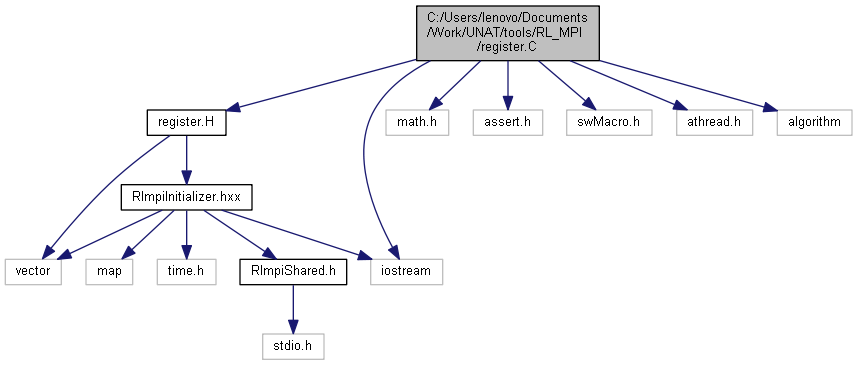
\includegraphics[width=350pt]{register_8C__incl}
\end{center}
\end{figure}
\subsection*{Functions}
\begin{DoxyCompactItemize}
\item 
void \mbox{\hyperlink{register_8C_aeb710bc88af64d82c952623c9082f060}{slave\+\_\+init\+Table}} (\mbox{\hyperlink{structRlmpiInfo}{Rlmpi\+Info}} $\ast$data)
\item 
void \mbox{\hyperlink{register_8C_a4e113cf30f6198d50fb212074effcc61}{init\+Send\+List}} (int $\ast$data\+Send\+List, int msh\+Block\+Num)
\item 
void \mbox{\hyperlink{register_8C_ace23239002b4fdf135d4ad20ae2df6e7}{init\+Send\+List}} (int $\ast$data\+Send\+List, vector$<$ vector$<$ int $>$ $>$ data\+List, int msh\+Block\+Num)
\item 
void \mbox{\hyperlink{register_8C_a14fad51cfceca5a582218c98bdb3d769}{init\+Table}} (int index)
\item 
void \mbox{\hyperlink{register_8C_a099f07ebad307cc1509766f32cfcba5f}{destroy\+Table}} (int index)
\end{DoxyCompactItemize}


\subsection{Function Documentation}
\mbox{\Hypertarget{register_8C_a099f07ebad307cc1509766f32cfcba5f}\label{register_8C_a099f07ebad307cc1509766f32cfcba5f}} 
\index{register.C@{register.C}!destroyTable@{destroyTable}}
\index{destroyTable@{destroyTable}!register.C@{register.C}}
\subsubsection{\texorpdfstring{destroyTable()}{destroyTable()}}
{\footnotesize\ttfamily void destroy\+Table (\begin{DoxyParamCaption}\item[{int}]{index }\end{DoxyParamCaption})}

Here is the call graph for this function\+:
\nopagebreak
\begin{figure}[H]
\begin{center}
\leavevmode
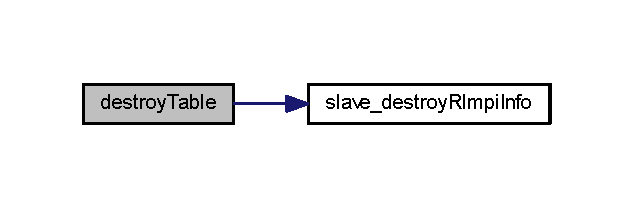
\includegraphics[width=304pt]{register_8C_a099f07ebad307cc1509766f32cfcba5f_cgraph}
\end{center}
\end{figure}
\mbox{\Hypertarget{register_8C_a4e113cf30f6198d50fb212074effcc61}\label{register_8C_a4e113cf30f6198d50fb212074effcc61}} 
\index{register.C@{register.C}!initSendList@{initSendList}}
\index{initSendList@{initSendList}!register.C@{register.C}}
\subsubsection{\texorpdfstring{initSendList()}{initSendList()}\hspace{0.1cm}{\footnotesize\ttfamily [1/2]}}
{\footnotesize\ttfamily void init\+Send\+List (\begin{DoxyParamCaption}\item[{int $\ast$}]{data\+Send\+List,  }\item[{int}]{msh\+Block\+Num }\end{DoxyParamCaption})}

Here is the call graph for this function\+:
\nopagebreak
\begin{figure}[H]
\begin{center}
\leavevmode
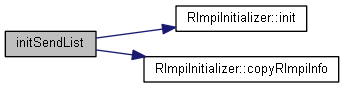
\includegraphics[width=330pt]{register_8C_a4e113cf30f6198d50fb212074effcc61_cgraph}
\end{center}
\end{figure}
\mbox{\Hypertarget{register_8C_ace23239002b4fdf135d4ad20ae2df6e7}\label{register_8C_ace23239002b4fdf135d4ad20ae2df6e7}} 
\index{register.C@{register.C}!initSendList@{initSendList}}
\index{initSendList@{initSendList}!register.C@{register.C}}
\subsubsection{\texorpdfstring{initSendList()}{initSendList()}\hspace{0.1cm}{\footnotesize\ttfamily [2/2]}}
{\footnotesize\ttfamily void init\+Send\+List (\begin{DoxyParamCaption}\item[{int $\ast$}]{data\+Send\+List,  }\item[{vector$<$ vector$<$ int $>$ $>$}]{data\+List,  }\item[{int}]{msh\+Block\+Num }\end{DoxyParamCaption})}

Here is the call graph for this function\+:
\nopagebreak
\begin{figure}[H]
\begin{center}
\leavevmode
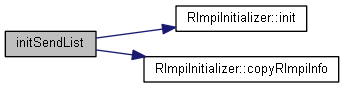
\includegraphics[width=330pt]{register_8C_ace23239002b4fdf135d4ad20ae2df6e7_cgraph}
\end{center}
\end{figure}
\mbox{\Hypertarget{register_8C_a14fad51cfceca5a582218c98bdb3d769}\label{register_8C_a14fad51cfceca5a582218c98bdb3d769}} 
\index{register.C@{register.C}!initTable@{initTable}}
\index{initTable@{initTable}!register.C@{register.C}}
\subsubsection{\texorpdfstring{initTable()}{initTable()}}
{\footnotesize\ttfamily void init\+Table (\begin{DoxyParamCaption}\item[{int}]{index }\end{DoxyParamCaption})}

Here is the call graph for this function\+:
\nopagebreak
\begin{figure}[H]
\begin{center}
\leavevmode
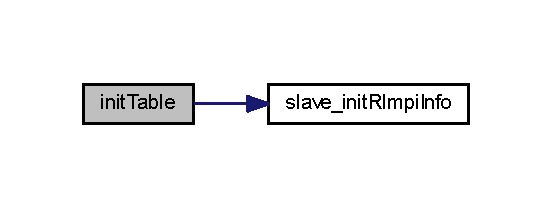
\includegraphics[width=265pt]{register_8C_a14fad51cfceca5a582218c98bdb3d769_cgraph}
\end{center}
\end{figure}
\mbox{\Hypertarget{register_8C_aeb710bc88af64d82c952623c9082f060}\label{register_8C_aeb710bc88af64d82c952623c9082f060}} 
\index{register.C@{register.C}!slave\_initTable@{slave\_initTable}}
\index{slave\_initTable@{slave\_initTable}!register.C@{register.C}}
\subsubsection{\texorpdfstring{slave\_initTable()}{slave\_initTable()}}
{\footnotesize\ttfamily void slave\+\_\+init\+Table (\begin{DoxyParamCaption}\item[{\mbox{\hyperlink{structRlmpiInfo}{Rlmpi\+Info}} $\ast$}]{data }\end{DoxyParamCaption})}

Here is the caller graph for this function\+:
\nopagebreak
\begin{figure}[H]
\begin{center}
\leavevmode
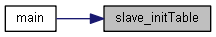
\includegraphics[width=234pt]{register_8C_aeb710bc88af64d82c952623c9082f060_icgraph}
\end{center}
\end{figure}

\hypertarget{register_8H}{
\section{RL\_\-MPI/register.H File Reference}
\label{register_8H}\index{RL\_\-MPI/register.H@{RL\_\-MPI/register.H}}
}
{\ttfamily \#include \char`\"{}RlmpiInitializer.hxx\char`\"{}}\par
\subsection*{Functions}
\begin{DoxyCompactItemize}
\item 
void \hyperlink{register_8H_a4e113cf30f6198d50fb212074effcc61}{initSendList} (int $\ast$dataSendList, int \hyperlink{edge2VertexIter__host_8c_ab5823517d185e26f48dc14ee05b60877}{mshBlockNum})
\item 
void \hyperlink{register_8H_a14fad51cfceca5a582218c98bdb3d769}{initTable} (int index)
\item 
void \hyperlink{register_8H_a099f07ebad307cc1509766f32cfcba5f}{destroyTable} (int index)
\end{DoxyCompactItemize}
\subsection*{Variables}
\begin{DoxyCompactItemize}
\item 
\hyperlink{structSchedule}{Schedule} $\ast$ \hyperlink{register_8H_ae191ced1f6c194db9b7dc5c3aed3a5d2}{schedule\_\-data}
\end{DoxyCompactItemize}


\subsection{Function Documentation}
\hypertarget{register_8H_a099f07ebad307cc1509766f32cfcba5f}{
\index{register.H@{register.H}!destroyTable@{destroyTable}}
\index{destroyTable@{destroyTable}!register.H@{register.H}}
\subsubsection[{destroyTable}]{\setlength{\rightskip}{0pt plus 5cm}void destroyTable (int {\em index})}}
\label{register_8H_a099f07ebad307cc1509766f32cfcba5f}
\hypertarget{register_8H_a4e113cf30f6198d50fb212074effcc61}{
\index{register.H@{register.H}!initSendList@{initSendList}}
\index{initSendList@{initSendList}!register.H@{register.H}}
\subsubsection[{initSendList}]{\setlength{\rightskip}{0pt plus 5cm}void initSendList (int $\ast$ {\em dataSendList}, \/  int {\em mshBlockNum})}}
\label{register_8H_a4e113cf30f6198d50fb212074effcc61}
\hypertarget{register_8H_a14fad51cfceca5a582218c98bdb3d769}{
\index{register.H@{register.H}!initTable@{initTable}}
\index{initTable@{initTable}!register.H@{register.H}}
\subsubsection[{initTable}]{\setlength{\rightskip}{0pt plus 5cm}void initTable (int {\em index})}}
\label{register_8H_a14fad51cfceca5a582218c98bdb3d769}


\subsection{Variable Documentation}
\hypertarget{register_8H_ae191ced1f6c194db9b7dc5c3aed3a5d2}{
\index{register.H@{register.H}!schedule\_\-data@{schedule\_\-data}}
\index{schedule\_\-data@{schedule\_\-data}!register.H@{register.H}}
\subsubsection[{schedule\_\-data}]{\setlength{\rightskip}{0pt plus 5cm}{\bf Schedule}$\ast$ {\bf schedule\_\-data}}}
\label{register_8H_ae191ced1f6c194db9b7dc5c3aed3a5d2}

\hypertarget{rlmpi_8c}{}\section{C\+:/\+Users/lenovo/\+Documents/\+Work/\+U\+N\+A\+T/tools/\+R\+L\+\_\+\+M\+P\+I/rlmpi.c File Reference}
\label{rlmpi_8c}\index{C:/Users/lenovo/Documents/Work/UNAT/tools/RL\_MPI/rlmpi.c@{C:/Users/lenovo/Documents/Work/UNAT/tools/RL\_MPI/rlmpi.c}}
{\ttfamily \#include $<$slave.\+h$>$}\newline
{\ttfamily \#include $<$dma.\+h$>$}\newline
{\ttfamily \#include $<$unistd.\+h$>$}\newline
{\ttfamily \#include $<$simd.\+h$>$}\newline
{\ttfamily \#include \char`\"{}Rlmpi\+Shared.\+h\char`\"{}}\newline
{\ttfamily \#include \char`\"{}rlmpi.\+h\char`\"{}}\newline
Include dependency graph for rlmpi.\+c\+:
\nopagebreak
\begin{figure}[H]
\begin{center}
\leavevmode
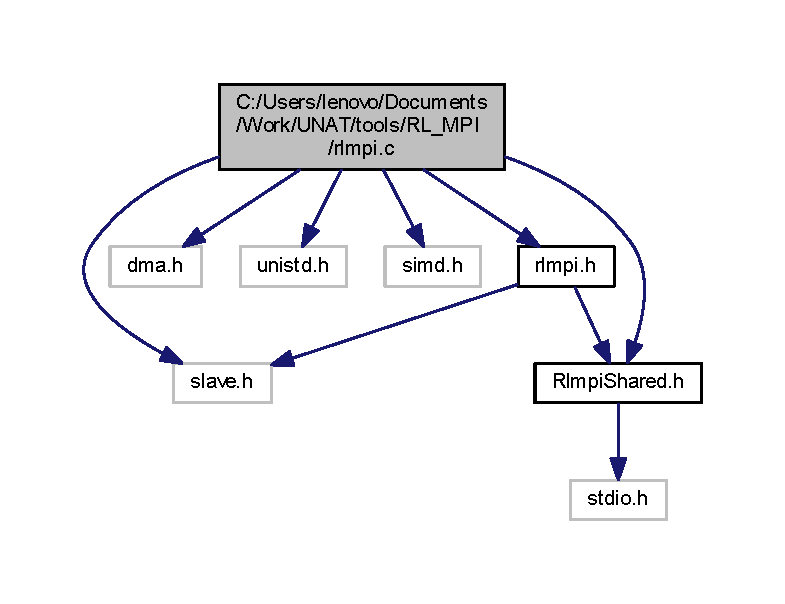
\includegraphics[width=350pt]{rlmpi_8c__incl}
\end{center}
\end{figure}
\subsection*{Macros}
\begin{DoxyCompactItemize}
\item 
\#define \mbox{\hyperlink{rlmpi_8c_a137869a1060d9043724de194e3c80ed5}{F\+I\+L\+E\+\_\+\+R\+L\+M\+P\+I\+\_\+C}}
\end{DoxyCompactItemize}
\subsection*{Functions}
\begin{DoxyCompactItemize}
\item 
\+\_\+\+\_\+thread\+\_\+local\+\_\+fix volatile \mbox{\hyperlink{rlmpi_8c_a284980254ff9c5412353987744875c1d}{\+\_\+\+\_\+attribute\+\_\+\+\_\+}} ((aligned(32)))
\item 
int \mbox{\hyperlink{rlmpi_8c_a37563f9d432c8bc4e9840a1dc2d9d294}{largerest}} (int a, int b, int c)
\item 
int \mbox{\hyperlink{rlmpi_8c_a16fb0107c31692875e7e6a614a40b97d}{Ceil}} (int a, int b)
\item 
int \mbox{\hyperlink{rlmpi_8c_a2cafae399ac0045562f1ef979050f5a8}{get\+\_\+aligned\+\_\+length}} (int len)
\item 
void \mbox{\hyperlink{rlmpi_8c_a8dbfac247f72ffdc0ea728a0186c7fd4}{load\+\_\+rlmpi\+\_\+data}} (\mbox{\hyperlink{structRlmpiInfo}{Rlmpi\+Info}} $\ast$rlmpi\+\_\+info)
\item 
void \mbox{\hyperlink{rlmpi_8c_a60189c7b674f63eeb9471a3d3f99c016}{load\+\_\+rlmpi\+\_\+data2}} (\mbox{\hyperlink{structRlmpiInfo}{Rlmpi\+Info}} $\ast$rlmpi\+\_\+info)
\item 
void \mbox{\hyperlink{rlmpi_8c_aaefd5bd835409949e03af9c3e0cff2c2}{destroy\+Rlmpi\+Info}} (\mbox{\hyperlink{structRlmpiInfo}{Rlmpi\+Info}} $\ast$rlmpi\+\_\+info)
\item 
void \mbox{\hyperlink{rlmpi_8c_acfbe467d1f994ed35c8f5fa9d42f360f}{init\+Rlmpi\+Info}} (\mbox{\hyperlink{structRlmpiInfo}{Rlmpi\+Info}} $\ast$rlmpi\+\_\+info)
\item 
void \mbox{\hyperlink{rlmpi_8c_a64e75a49b18fde131c205e5a74240184}{Transform\+Package\+Skew}} (const Pack $\ast$s\+Packs\+\_\+, Pack $\ast$r\+Packs\+\_\+)
\item 
void \mbox{\hyperlink{rlmpi_8c_a769393193e5b7cba40dc1855348a7e53}{Transform\+Same\+Row\+Package}} (const Pack $\ast$s\+Packs, Pack $\ast$r\+Packs)
\item 
void \mbox{\hyperlink{rlmpi_8c_af6301fe17756b6d8df9963b6bd08fa07}{Transform\+Same\+Column\+Package}} (const Pack $\ast$s\+Packs, Pack $\ast$r\+Packs)
\item 
void \mbox{\hyperlink{rlmpi_8c_a2839a0d31161d2024e67dc2e6c13ad8c}{sort\+\_\+recv\+\_\+package}} (Pack $\ast$r\+Packs\+\_\+, int npack)
\item 
void \mbox{\hyperlink{rlmpi_8c_aa78bcd4175a6642b9c9b55388d2e70e4}{transform\+\_\+data}} ()
\end{DoxyCompactItemize}


\subsection{Macro Definition Documentation}
\mbox{\Hypertarget{rlmpi_8c_a137869a1060d9043724de194e3c80ed5}\label{rlmpi_8c_a137869a1060d9043724de194e3c80ed5}} 
\index{rlmpi.c@{rlmpi.c}!FILE\_RLMPI\_C@{FILE\_RLMPI\_C}}
\index{FILE\_RLMPI\_C@{FILE\_RLMPI\_C}!rlmpi.c@{rlmpi.c}}
\subsubsection{\texorpdfstring{FILE\_RLMPI\_C}{FILE\_RLMPI\_C}}
{\footnotesize\ttfamily \#define F\+I\+L\+E\+\_\+\+R\+L\+M\+P\+I\+\_\+C}



\subsection{Function Documentation}
\mbox{\Hypertarget{rlmpi_8c_a284980254ff9c5412353987744875c1d}\label{rlmpi_8c_a284980254ff9c5412353987744875c1d}} 
\index{rlmpi.c@{rlmpi.c}!\_\_attribute\_\_@{\_\_attribute\_\_}}
\index{\_\_attribute\_\_@{\_\_attribute\_\_}!rlmpi.c@{rlmpi.c}}
\subsubsection{\texorpdfstring{\_\_attribute\_\_()}{\_\_attribute\_\_()}}
{\footnotesize\ttfamily \+\_\+\+\_\+thread\+\_\+local\+\_\+fix volatile \mbox{\hyperlink{struct____attribute____}{\+\_\+\+\_\+attribute\+\_\+\+\_\+}} (\begin{DoxyParamCaption}\item[{(aligned(32))}]{ }\end{DoxyParamCaption})}

\mbox{\Hypertarget{rlmpi_8c_a16fb0107c31692875e7e6a614a40b97d}\label{rlmpi_8c_a16fb0107c31692875e7e6a614a40b97d}} 
\index{rlmpi.c@{rlmpi.c}!Ceil@{Ceil}}
\index{Ceil@{Ceil}!rlmpi.c@{rlmpi.c}}
\subsubsection{\texorpdfstring{Ceil()}{Ceil()}}
{\footnotesize\ttfamily int Ceil (\begin{DoxyParamCaption}\item[{int}]{a,  }\item[{int}]{b }\end{DoxyParamCaption})\hspace{0.3cm}{\ttfamily [inline]}}

Here is the caller graph for this function\+:
\nopagebreak
\begin{figure}[H]
\begin{center}
\leavevmode
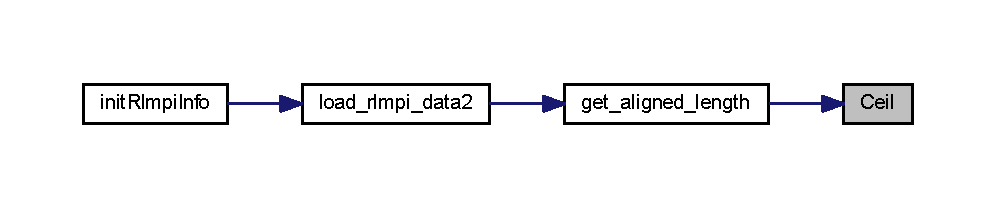
\includegraphics[width=350pt]{rlmpi_8c_a16fb0107c31692875e7e6a614a40b97d_icgraph}
\end{center}
\end{figure}
\mbox{\Hypertarget{rlmpi_8c_aaefd5bd835409949e03af9c3e0cff2c2}\label{rlmpi_8c_aaefd5bd835409949e03af9c3e0cff2c2}} 
\index{rlmpi.c@{rlmpi.c}!destroyRlmpiInfo@{destroyRlmpiInfo}}
\index{destroyRlmpiInfo@{destroyRlmpiInfo}!rlmpi.c@{rlmpi.c}}
\subsubsection{\texorpdfstring{destroyRlmpiInfo()}{destroyRlmpiInfo()}}
{\footnotesize\ttfamily void destroy\+Rlmpi\+Info (\begin{DoxyParamCaption}\item[{\mbox{\hyperlink{structRlmpiInfo}{Rlmpi\+Info}} $\ast$}]{rlmpi\+\_\+info }\end{DoxyParamCaption})}

\mbox{\Hypertarget{rlmpi_8c_a2cafae399ac0045562f1ef979050f5a8}\label{rlmpi_8c_a2cafae399ac0045562f1ef979050f5a8}} 
\index{rlmpi.c@{rlmpi.c}!get\_aligned\_length@{get\_aligned\_length}}
\index{get\_aligned\_length@{get\_aligned\_length}!rlmpi.c@{rlmpi.c}}
\subsubsection{\texorpdfstring{get\_aligned\_length()}{get\_aligned\_length()}}
{\footnotesize\ttfamily int get\+\_\+aligned\+\_\+length (\begin{DoxyParamCaption}\item[{int}]{len }\end{DoxyParamCaption})\hspace{0.3cm}{\ttfamily [inline]}}

Here is the call graph for this function\+:
\nopagebreak
\begin{figure}[H]
\begin{center}
\leavevmode
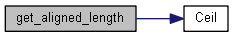
\includegraphics[width=247pt]{rlmpi_8c_a2cafae399ac0045562f1ef979050f5a8_cgraph}
\end{center}
\end{figure}
Here is the caller graph for this function\+:
\nopagebreak
\begin{figure}[H]
\begin{center}
\leavevmode
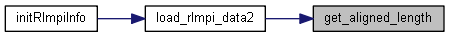
\includegraphics[width=350pt]{rlmpi_8c_a2cafae399ac0045562f1ef979050f5a8_icgraph}
\end{center}
\end{figure}
\mbox{\Hypertarget{rlmpi_8c_acfbe467d1f994ed35c8f5fa9d42f360f}\label{rlmpi_8c_acfbe467d1f994ed35c8f5fa9d42f360f}} 
\index{rlmpi.c@{rlmpi.c}!initRlmpiInfo@{initRlmpiInfo}}
\index{initRlmpiInfo@{initRlmpiInfo}!rlmpi.c@{rlmpi.c}}
\subsubsection{\texorpdfstring{initRlmpiInfo()}{initRlmpiInfo()}}
{\footnotesize\ttfamily void init\+Rlmpi\+Info (\begin{DoxyParamCaption}\item[{\mbox{\hyperlink{structRlmpiInfo}{Rlmpi\+Info}} $\ast$}]{rlmpi\+\_\+info }\end{DoxyParamCaption})}

Here is the call graph for this function\+:
\nopagebreak
\begin{figure}[H]
\begin{center}
\leavevmode
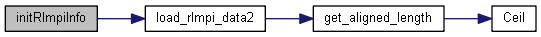
\includegraphics[width=350pt]{rlmpi_8c_acfbe467d1f994ed35c8f5fa9d42f360f_cgraph}
\end{center}
\end{figure}
\mbox{\Hypertarget{rlmpi_8c_a37563f9d432c8bc4e9840a1dc2d9d294}\label{rlmpi_8c_a37563f9d432c8bc4e9840a1dc2d9d294}} 
\index{rlmpi.c@{rlmpi.c}!largerest@{largerest}}
\index{largerest@{largerest}!rlmpi.c@{rlmpi.c}}
\subsubsection{\texorpdfstring{largerest()}{largerest()}}
{\footnotesize\ttfamily int largerest (\begin{DoxyParamCaption}\item[{int}]{a,  }\item[{int}]{b,  }\item[{int}]{c }\end{DoxyParamCaption})\hspace{0.3cm}{\ttfamily [inline]}}

\mbox{\Hypertarget{rlmpi_8c_a8dbfac247f72ffdc0ea728a0186c7fd4}\label{rlmpi_8c_a8dbfac247f72ffdc0ea728a0186c7fd4}} 
\index{rlmpi.c@{rlmpi.c}!load\_rlmpi\_data@{load\_rlmpi\_data}}
\index{load\_rlmpi\_data@{load\_rlmpi\_data}!rlmpi.c@{rlmpi.c}}
\subsubsection{\texorpdfstring{load\_rlmpi\_data()}{load\_rlmpi\_data()}}
{\footnotesize\ttfamily void load\+\_\+rlmpi\+\_\+data (\begin{DoxyParamCaption}\item[{\mbox{\hyperlink{structRlmpiInfo}{Rlmpi\+Info}} $\ast$}]{rlmpi\+\_\+info }\end{DoxyParamCaption})\hspace{0.3cm}{\ttfamily [inline]}}

\mbox{\Hypertarget{rlmpi_8c_a60189c7b674f63eeb9471a3d3f99c016}\label{rlmpi_8c_a60189c7b674f63eeb9471a3d3f99c016}} 
\index{rlmpi.c@{rlmpi.c}!load\_rlmpi\_data2@{load\_rlmpi\_data2}}
\index{load\_rlmpi\_data2@{load\_rlmpi\_data2}!rlmpi.c@{rlmpi.c}}
\subsubsection{\texorpdfstring{load\_rlmpi\_data2()}{load\_rlmpi\_data2()}}
{\footnotesize\ttfamily void load\+\_\+rlmpi\+\_\+data2 (\begin{DoxyParamCaption}\item[{\mbox{\hyperlink{structRlmpiInfo}{Rlmpi\+Info}} $\ast$}]{rlmpi\+\_\+info }\end{DoxyParamCaption})\hspace{0.3cm}{\ttfamily [inline]}}

Here is the call graph for this function\+:
\nopagebreak
\begin{figure}[H]
\begin{center}
\leavevmode
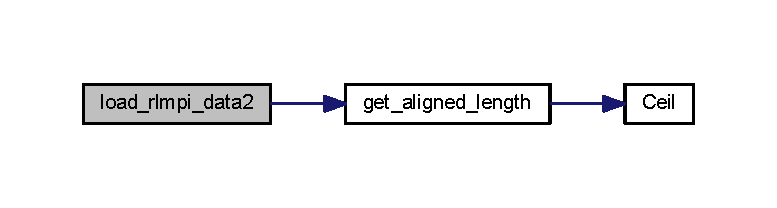
\includegraphics[width=350pt]{rlmpi_8c_a60189c7b674f63eeb9471a3d3f99c016_cgraph}
\end{center}
\end{figure}
Here is the caller graph for this function\+:
\nopagebreak
\begin{figure}[H]
\begin{center}
\leavevmode
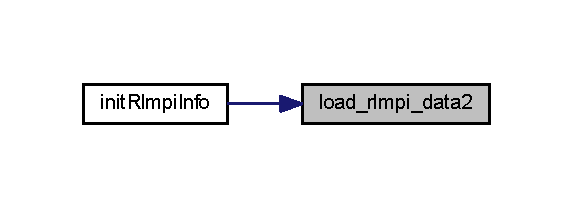
\includegraphics[width=275pt]{rlmpi_8c_a60189c7b674f63eeb9471a3d3f99c016_icgraph}
\end{center}
\end{figure}
\mbox{\Hypertarget{rlmpi_8c_a2839a0d31161d2024e67dc2e6c13ad8c}\label{rlmpi_8c_a2839a0d31161d2024e67dc2e6c13ad8c}} 
\index{rlmpi.c@{rlmpi.c}!sort\_recv\_package@{sort\_recv\_package}}
\index{sort\_recv\_package@{sort\_recv\_package}!rlmpi.c@{rlmpi.c}}
\subsubsection{\texorpdfstring{sort\_recv\_package()}{sort\_recv\_package()}}
{\footnotesize\ttfamily void sort\+\_\+recv\+\_\+package (\begin{DoxyParamCaption}\item[{Pack $\ast$}]{r\+Packs\+\_\+,  }\item[{int}]{npack }\end{DoxyParamCaption})\hspace{0.3cm}{\ttfamily [inline]}}

\mbox{\Hypertarget{rlmpi_8c_aa78bcd4175a6642b9c9b55388d2e70e4}\label{rlmpi_8c_aa78bcd4175a6642b9c9b55388d2e70e4}} 
\index{rlmpi.c@{rlmpi.c}!transform\_data@{transform\_data}}
\index{transform\_data@{transform\_data}!rlmpi.c@{rlmpi.c}}
\subsubsection{\texorpdfstring{transform\_data()}{transform\_data()}}
{\footnotesize\ttfamily void transform\+\_\+data (\begin{DoxyParamCaption}{ }\end{DoxyParamCaption})\hspace{0.3cm}{\ttfamily [inline]}}

Here is the call graph for this function\+:
\nopagebreak
\begin{figure}[H]
\begin{center}
\leavevmode
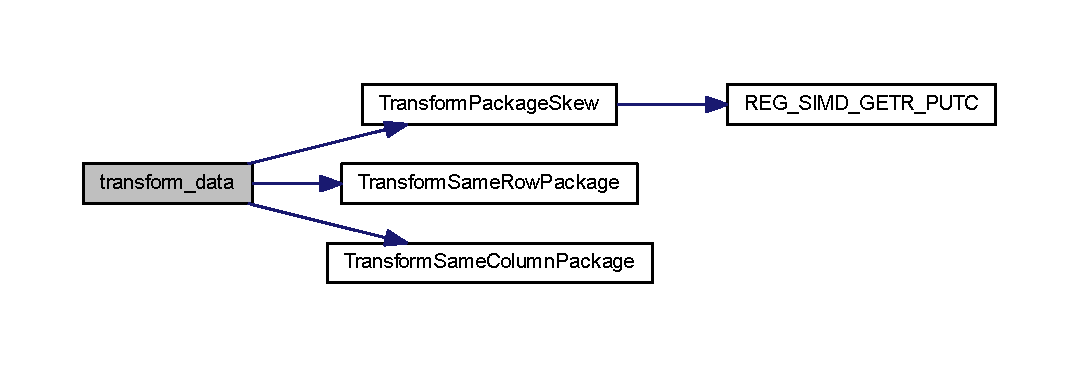
\includegraphics[width=350pt]{rlmpi_8c_aa78bcd4175a6642b9c9b55388d2e70e4_cgraph}
\end{center}
\end{figure}
Here is the caller graph for this function\+:
\nopagebreak
\begin{figure}[H]
\begin{center}
\leavevmode
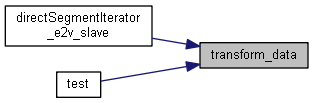
\includegraphics[width=307pt]{rlmpi_8c_aa78bcd4175a6642b9c9b55388d2e70e4_icgraph}
\end{center}
\end{figure}
\mbox{\Hypertarget{rlmpi_8c_a64e75a49b18fde131c205e5a74240184}\label{rlmpi_8c_a64e75a49b18fde131c205e5a74240184}} 
\index{rlmpi.c@{rlmpi.c}!TransformPackageSkew@{TransformPackageSkew}}
\index{TransformPackageSkew@{TransformPackageSkew}!rlmpi.c@{rlmpi.c}}
\subsubsection{\texorpdfstring{TransformPackageSkew()}{TransformPackageSkew()}}
{\footnotesize\ttfamily void Transform\+Package\+Skew (\begin{DoxyParamCaption}\item[{const Pack $\ast$}]{s\+Packs\+\_\+,  }\item[{Pack $\ast$}]{r\+Packs\+\_\+ }\end{DoxyParamCaption})\hspace{0.3cm}{\ttfamily [inline]}}

Here is the call graph for this function\+:
\nopagebreak
\begin{figure}[H]
\begin{center}
\leavevmode
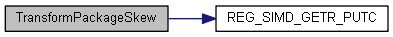
\includegraphics[width=350pt]{rlmpi_8c_a64e75a49b18fde131c205e5a74240184_cgraph}
\end{center}
\end{figure}
\mbox{\Hypertarget{rlmpi_8c_af6301fe17756b6d8df9963b6bd08fa07}\label{rlmpi_8c_af6301fe17756b6d8df9963b6bd08fa07}} 
\index{rlmpi.c@{rlmpi.c}!TransformSameColumnPackage@{TransformSameColumnPackage}}
\index{TransformSameColumnPackage@{TransformSameColumnPackage}!rlmpi.c@{rlmpi.c}}
\subsubsection{\texorpdfstring{TransformSameColumnPackage()}{TransformSameColumnPackage()}}
{\footnotesize\ttfamily void Transform\+Same\+Column\+Package (\begin{DoxyParamCaption}\item[{const Pack $\ast$}]{s\+Packs,  }\item[{Pack $\ast$}]{r\+Packs }\end{DoxyParamCaption})\hspace{0.3cm}{\ttfamily [inline]}}

\mbox{\Hypertarget{rlmpi_8c_a769393193e5b7cba40dc1855348a7e53}\label{rlmpi_8c_a769393193e5b7cba40dc1855348a7e53}} 
\index{rlmpi.c@{rlmpi.c}!TransformSameRowPackage@{TransformSameRowPackage}}
\index{TransformSameRowPackage@{TransformSameRowPackage}!rlmpi.c@{rlmpi.c}}
\subsubsection{\texorpdfstring{TransformSameRowPackage()}{TransformSameRowPackage()}}
{\footnotesize\ttfamily void Transform\+Same\+Row\+Package (\begin{DoxyParamCaption}\item[{const Pack $\ast$}]{s\+Packs,  }\item[{Pack $\ast$}]{r\+Packs }\end{DoxyParamCaption})\hspace{0.3cm}{\ttfamily [inline]}}


\hypertarget{rlmpi_8h}{
\section{RL\_\-MPI/rlmpi.h File Reference}
\label{rlmpi_8h}\index{RL\_\-MPI/rlmpi.h@{RL\_\-MPI/rlmpi.h}}
}
{\ttfamily \#include $<$slave.h$>$}\par
{\ttfamily \#include \char`\"{}RlmpiSharedType.h\char`\"{}}\par
\subsection*{Defines}
\begin{DoxyCompactItemize}
\item 
\#define \hyperlink{rlmpi_8h_a745a07191e6ec137237667d0cd337e91}{MaxNPackages}~450
\item 
\#define \hyperlink{rlmpi_8h_a77c1dce4fdc3220f82f422eaef22fe6f}{MaxNCycle}~200
\item 
\#define \hyperlink{rlmpi_8h_aa3c66c548e5929072bcf5178486bbb56}{MaxNElm}~35
\item 
\#define \hyperlink{rlmpi_8h_a005b28da29b25c5a55ed78e4b734bee6}{COL}(\hyperlink{edge2VertexIter__slave_8c_aa1f0f95cf24b79e2f4f341a3a492940e}{x})~(\hyperlink{edge2VertexIter__slave_8c_aa1f0f95cf24b79e2f4f341a3a492940e}{x} \& 0x07)
\item 
\#define \hyperlink{rlmpi_8h_a24630bb1cd43b553e14df6af1beba35c}{ROW}(\hyperlink{edge2VertexIter__slave_8c_aa1f0f95cf24b79e2f4f341a3a492940e}{x})~((\hyperlink{edge2VertexIter__slave_8c_aa1f0f95cf24b79e2f4f341a3a492940e}{x} \& 0x38) $>$$>$ 3)
\item 
\#define \hyperlink{rlmpi_8h_ab64860068dc86584eda905e83ed6c960}{REG\_\-PUTR}(var, dst)~asm volatile (\char`\"{}putr \%0,\%1$\backslash$n\char`\"{}::\char`\"{}r\char`\"{}(var),\char`\"{}r\char`\"{}(dst):\char`\"{}memory\char`\"{})
\item 
\#define \hyperlink{rlmpi_8h_a146c2d765e771d3fefd08c5598044d63}{REG\_\-PUTC}(var, dst)~asm volatile (\char`\"{}putc \%0,\%1$\backslash$n\char`\"{}::\char`\"{}r\char`\"{}(var),\char`\"{}r\char`\"{}(dst):\char`\"{}memory\char`\"{})
\item 
\#define \hyperlink{rlmpi_8h_abf0ab377d13927e4a0d3561fe7303225}{REG\_\-GETR}(var)~asm volatile (\char`\"{}getr \%0$\backslash$n\char`\"{}:\char`\"{}=r\char`\"{}(var)::\char`\"{}memory\char`\"{})
\item 
\#define \hyperlink{rlmpi_8h_a322b72e0fd0822f674c04690f0701f03}{REG\_\-GETC}(var)~asm volatile (\char`\"{}getc \%0$\backslash$n\char`\"{}:\char`\"{}=r\char`\"{}(var)::\char`\"{}memory\char`\"{})
\item 
\#define \hyperlink{rlmpi_8h_ac037a5aa71fbb49e8a31955ef25d1657}{REG\_\-SIMD\_\-PUTR}(var, dst)~asm volatile (\char`\"{}putr \%0,\%1$\backslash$n\char`\"{}::\char`\"{}r\char`\"{}(var),\char`\"{}r\char`\"{}(dst):\char`\"{}memory\char`\"{})
\item 
\#define \hyperlink{rlmpi_8h_ae338ed428d7ceaf9e639e68049eb040b}{REG\_\-SIMD\_\-PUTC}(var, dst)~asm volatile (\char`\"{}putc \%0,\%1$\backslash$n\char`\"{}::\char`\"{}r\char`\"{}(var),\char`\"{}r\char`\"{}(dst):\char`\"{}memory\char`\"{})
\item 
\#define \hyperlink{rlmpi_8h_a4869a4bef56a19c0ec139363da0bbedc}{REG\_\-SIMD\_\-GETR}(var)~asm volatile (\char`\"{}getr \%0$\backslash$n\char`\"{}:\char`\"{}=r\char`\"{}(var)::\char`\"{}memory\char`\"{})
\item 
\#define \hyperlink{rlmpi_8h_adc6e2805f8e23324f95f6c2e853fdc56}{REG\_\-SIMD\_\-GETC}(var)~asm volatile (\char`\"{}getc \%0$\backslash$n\char`\"{}:\char`\"{}=r\char`\"{}(var)::\char`\"{}memory\char`\"{})
\item 
\#define \hyperlink{rlmpi_8h_a836954365267363366cfc2ead0190bf2}{ROWSYN}~athread\_\-syn(ROW\_\-SCOPE,0xff)
\item 
\#define \hyperlink{rlmpi_8h_abc486310daaebe2e7c69775b43c1a14a}{COLSYN}~athread\_\-syn(COL\_\-SCOPE,0xff)
\item 
\#define \hyperlink{rlmpi_8h_a9ce21ca82ef32711a9edf81360a796ef}{ALLSYN}~athread\_\-syn(ARRAY\_\-SCOPE,0xffff)
\end{DoxyCompactItemize}
\subsection*{Functions}
\begin{DoxyCompactItemize}
\item 
\_\-\_\-thread\_\-local\_\-fix volatile \hyperlink{rlmpi_8h_a2d18c9cdfe552606a5516503d1262b3c}{\_\-\_\-attribute\_\-\_\-} ((aligned(32))) \hyperlink{RlmpiSharedType_8h_a69782ffde89d45e86308f10afedf08a6}{int8LDM} \_\-putr\_\-schedules\mbox{[}MaxNCycle\mbox{]}
\item 
void \hyperlink{rlmpi_8h_ab1d809714600f31478edf8d1f6466970}{TransformPackage3} (const Pack $\ast$sPacks, Pack $\ast$rPacks)
\item 
void \hyperlink{rlmpi_8h_af6301fe17756b6d8df9963b6bd08fa07}{TransformSameColumnPackage} (const Pack $\ast$sPacks, Pack $\ast$rPacks)
\item 
void \hyperlink{rlmpi_8h_a769393193e5b7cba40dc1855348a7e53}{TransformSameRowPackage} (const Pack $\ast$sPacks, Pack $\ast$rPacks)
\item 
void \hyperlink{rlmpi_8h_af08d9249e0be638ee065314f38c52984}{load\_\-reg\_\-mpi\_\-init\_\-data} (\hyperlink{structSchedule}{Schedule} $\ast$reg\_\-data)
\item 
void \hyperlink{rlmpi_8h_a29c1a70b4be837c1771603fe8463bff3}{REG\_\-SIMD\_\-GETR\_\-PUTC} ()
\end{DoxyCompactItemize}
\subsection*{Variables}
\begin{DoxyCompactItemize}
\item 
\_\-\_\-thread\_\-local\_\-fix Pack \hyperlink{rlmpi_8h_a7fc545f3109555c8d51483cc95a328d9}{\_\-sPacks} \mbox{[}MaxNPackages\mbox{]}
\item 
\_\-\_\-thread\_\-local\_\-fix Pack \hyperlink{rlmpi_8h_af9c1ffbc340d52cdb835be4c107bb080}{\_\-rPacks} \mbox{[}MaxNPackages\mbox{]}
\item 
\_\-\_\-thread\_\-local\_\-fix Pack $\ast$ \hyperlink{rlmpi_8h_a76928eeb9bbd93ccb4d1682181d5c7a7}{\_\-sPacks\_\-same\_\-col}
\item 
\_\-\_\-thread\_\-local\_\-fix Pack $\ast$ \hyperlink{rlmpi_8h_a8e8861831dec614d8a20ad93aae3c3c4}{\_\-sPacks\_\-same\_\-row}
\item 
\_\-\_\-thread\_\-local\_\-fix volatile Table \hyperlink{rlmpi_8h_af29a1368a7c478624ec26c60f22b9185}{\_\-table\_\-ldm}
\item 
\_\-\_\-thread\_\-local\_\-fix int \hyperlink{rlmpi_8h_a29b9f988cabc5af3c11611e8d2902733}{\_\-total\_\-send\_\-pcg}
\item 
\_\-\_\-thread\_\-local\_\-fix int \hyperlink{rlmpi_8h_aa4d7bc5a2f4130fe138bb39172901372}{\_\-total\_\-recv\_\-pcg}
\item 
\_\-\_\-thread\_\-local\_\-fix int \hyperlink{rlmpi_8h_a9fb1916d580795274f4b1b64eb7da0eb}{\_\-nCycle}
\item 
\_\-\_\-thread\_\-local\_\-fix int \hyperlink{rlmpi_8h_af222dfff432ce24c662f1ac54e6ea298}{\_\-nCycleSameCol}
\item 
\_\-\_\-thread\_\-local\_\-fix volatile int \hyperlink{rlmpi_8h_a4cf5e17b4998248b723ad313965af27d}{\_\-nCycleSameRow}
\item 
\_\-\_\-thread\_\-local int \hyperlink{rlmpi_8h_afcf1a06a5cf9e3464cadd07fd7f8a93e}{\_\-get\_\-reply}
\item 
\_\-\_\-thread\_\-local int \hyperlink{rlmpi_8h_ae71dd5187a7635b1e219d00e0d5f8c11}{\_\-put\_\-reply}
\end{DoxyCompactItemize}


\subsection{Define Documentation}
\hypertarget{rlmpi_8h_a9ce21ca82ef32711a9edf81360a796ef}{
\index{rlmpi.h@{rlmpi.h}!ALLSYN@{ALLSYN}}
\index{ALLSYN@{ALLSYN}!rlmpi.h@{rlmpi.h}}
\subsubsection[{ALLSYN}]{\setlength{\rightskip}{0pt plus 5cm}\#define ALLSYN~athread\_\-syn(ARRAY\_\-SCOPE,0xffff)}}
\label{rlmpi_8h_a9ce21ca82ef32711a9edf81360a796ef}
\hypertarget{rlmpi_8h_a005b28da29b25c5a55ed78e4b734bee6}{
\index{rlmpi.h@{rlmpi.h}!COL@{COL}}
\index{COL@{COL}!rlmpi.h@{rlmpi.h}}
\subsubsection[{COL}]{\setlength{\rightskip}{0pt plus 5cm}\#define COL({\bf x})~({\bf x} \& 0x07)}}
\label{rlmpi_8h_a005b28da29b25c5a55ed78e4b734bee6}
\hypertarget{rlmpi_8h_abc486310daaebe2e7c69775b43c1a14a}{
\index{rlmpi.h@{rlmpi.h}!COLSYN@{COLSYN}}
\index{COLSYN@{COLSYN}!rlmpi.h@{rlmpi.h}}
\subsubsection[{COLSYN}]{\setlength{\rightskip}{0pt plus 5cm}\#define COLSYN~athread\_\-syn(COL\_\-SCOPE,0xff)}}
\label{rlmpi_8h_abc486310daaebe2e7c69775b43c1a14a}
\hypertarget{rlmpi_8h_a77c1dce4fdc3220f82f422eaef22fe6f}{
\index{rlmpi.h@{rlmpi.h}!MaxNCycle@{MaxNCycle}}
\index{MaxNCycle@{MaxNCycle}!rlmpi.h@{rlmpi.h}}
\subsubsection[{MaxNCycle}]{\setlength{\rightskip}{0pt plus 5cm}\#define MaxNCycle~200}}
\label{rlmpi_8h_a77c1dce4fdc3220f82f422eaef22fe6f}
\hypertarget{rlmpi_8h_aa3c66c548e5929072bcf5178486bbb56}{
\index{rlmpi.h@{rlmpi.h}!MaxNElm@{MaxNElm}}
\index{MaxNElm@{MaxNElm}!rlmpi.h@{rlmpi.h}}
\subsubsection[{MaxNElm}]{\setlength{\rightskip}{0pt plus 5cm}\#define MaxNElm~35}}
\label{rlmpi_8h_aa3c66c548e5929072bcf5178486bbb56}
\hypertarget{rlmpi_8h_a745a07191e6ec137237667d0cd337e91}{
\index{rlmpi.h@{rlmpi.h}!MaxNPackages@{MaxNPackages}}
\index{MaxNPackages@{MaxNPackages}!rlmpi.h@{rlmpi.h}}
\subsubsection[{MaxNPackages}]{\setlength{\rightskip}{0pt plus 5cm}\#define MaxNPackages~450}}
\label{rlmpi_8h_a745a07191e6ec137237667d0cd337e91}
\hypertarget{rlmpi_8h_a322b72e0fd0822f674c04690f0701f03}{
\index{rlmpi.h@{rlmpi.h}!REG\_\-GETC@{REG\_\-GETC}}
\index{REG\_\-GETC@{REG\_\-GETC}!rlmpi.h@{rlmpi.h}}
\subsubsection[{REG\_\-GETC}]{\setlength{\rightskip}{0pt plus 5cm}\#define REG\_\-GETC(var)~asm volatile (\char`\"{}getc \%0$\backslash$n\char`\"{}:\char`\"{}=r\char`\"{}(var)::\char`\"{}memory\char`\"{})}}
\label{rlmpi_8h_a322b72e0fd0822f674c04690f0701f03}
\hypertarget{rlmpi_8h_abf0ab377d13927e4a0d3561fe7303225}{
\index{rlmpi.h@{rlmpi.h}!REG\_\-GETR@{REG\_\-GETR}}
\index{REG\_\-GETR@{REG\_\-GETR}!rlmpi.h@{rlmpi.h}}
\subsubsection[{REG\_\-GETR}]{\setlength{\rightskip}{0pt plus 5cm}\#define REG\_\-GETR(var)~asm volatile (\char`\"{}getr \%0$\backslash$n\char`\"{}:\char`\"{}=r\char`\"{}(var)::\char`\"{}memory\char`\"{})}}
\label{rlmpi_8h_abf0ab377d13927e4a0d3561fe7303225}
\hypertarget{rlmpi_8h_a146c2d765e771d3fefd08c5598044d63}{
\index{rlmpi.h@{rlmpi.h}!REG\_\-PUTC@{REG\_\-PUTC}}
\index{REG\_\-PUTC@{REG\_\-PUTC}!rlmpi.h@{rlmpi.h}}
\subsubsection[{REG\_\-PUTC}]{\setlength{\rightskip}{0pt plus 5cm}\#define REG\_\-PUTC(var, \/  dst)~asm volatile (\char`\"{}putc \%0,\%1$\backslash$n\char`\"{}::\char`\"{}r\char`\"{}(var),\char`\"{}r\char`\"{}(dst):\char`\"{}memory\char`\"{})}}
\label{rlmpi_8h_a146c2d765e771d3fefd08c5598044d63}
\hypertarget{rlmpi_8h_ab64860068dc86584eda905e83ed6c960}{
\index{rlmpi.h@{rlmpi.h}!REG\_\-PUTR@{REG\_\-PUTR}}
\index{REG\_\-PUTR@{REG\_\-PUTR}!rlmpi.h@{rlmpi.h}}
\subsubsection[{REG\_\-PUTR}]{\setlength{\rightskip}{0pt plus 5cm}\#define REG\_\-PUTR(var, \/  dst)~asm volatile (\char`\"{}putr \%0,\%1$\backslash$n\char`\"{}::\char`\"{}r\char`\"{}(var),\char`\"{}r\char`\"{}(dst):\char`\"{}memory\char`\"{})}}
\label{rlmpi_8h_ab64860068dc86584eda905e83ed6c960}
\hypertarget{rlmpi_8h_adc6e2805f8e23324f95f6c2e853fdc56}{
\index{rlmpi.h@{rlmpi.h}!REG\_\-SIMD\_\-GETC@{REG\_\-SIMD\_\-GETC}}
\index{REG\_\-SIMD\_\-GETC@{REG\_\-SIMD\_\-GETC}!rlmpi.h@{rlmpi.h}}
\subsubsection[{REG\_\-SIMD\_\-GETC}]{\setlength{\rightskip}{0pt plus 5cm}\#define REG\_\-SIMD\_\-GETC(var)~asm volatile (\char`\"{}getc \%0$\backslash$n\char`\"{}:\char`\"{}=r\char`\"{}(var)::\char`\"{}memory\char`\"{})}}
\label{rlmpi_8h_adc6e2805f8e23324f95f6c2e853fdc56}
\hypertarget{rlmpi_8h_a4869a4bef56a19c0ec139363da0bbedc}{
\index{rlmpi.h@{rlmpi.h}!REG\_\-SIMD\_\-GETR@{REG\_\-SIMD\_\-GETR}}
\index{REG\_\-SIMD\_\-GETR@{REG\_\-SIMD\_\-GETR}!rlmpi.h@{rlmpi.h}}
\subsubsection[{REG\_\-SIMD\_\-GETR}]{\setlength{\rightskip}{0pt plus 5cm}\#define REG\_\-SIMD\_\-GETR(var)~asm volatile (\char`\"{}getr \%0$\backslash$n\char`\"{}:\char`\"{}=r\char`\"{}(var)::\char`\"{}memory\char`\"{})}}
\label{rlmpi_8h_a4869a4bef56a19c0ec139363da0bbedc}
\hypertarget{rlmpi_8h_ae338ed428d7ceaf9e639e68049eb040b}{
\index{rlmpi.h@{rlmpi.h}!REG\_\-SIMD\_\-PUTC@{REG\_\-SIMD\_\-PUTC}}
\index{REG\_\-SIMD\_\-PUTC@{REG\_\-SIMD\_\-PUTC}!rlmpi.h@{rlmpi.h}}
\subsubsection[{REG\_\-SIMD\_\-PUTC}]{\setlength{\rightskip}{0pt plus 5cm}\#define REG\_\-SIMD\_\-PUTC(var, \/  dst)~asm volatile (\char`\"{}putc \%0,\%1$\backslash$n\char`\"{}::\char`\"{}r\char`\"{}(var),\char`\"{}r\char`\"{}(dst):\char`\"{}memory\char`\"{})}}
\label{rlmpi_8h_ae338ed428d7ceaf9e639e68049eb040b}
\hypertarget{rlmpi_8h_ac037a5aa71fbb49e8a31955ef25d1657}{
\index{rlmpi.h@{rlmpi.h}!REG\_\-SIMD\_\-PUTR@{REG\_\-SIMD\_\-PUTR}}
\index{REG\_\-SIMD\_\-PUTR@{REG\_\-SIMD\_\-PUTR}!rlmpi.h@{rlmpi.h}}
\subsubsection[{REG\_\-SIMD\_\-PUTR}]{\setlength{\rightskip}{0pt plus 5cm}\#define REG\_\-SIMD\_\-PUTR(var, \/  dst)~asm volatile (\char`\"{}putr \%0,\%1$\backslash$n\char`\"{}::\char`\"{}r\char`\"{}(var),\char`\"{}r\char`\"{}(dst):\char`\"{}memory\char`\"{})}}
\label{rlmpi_8h_ac037a5aa71fbb49e8a31955ef25d1657}
\hypertarget{rlmpi_8h_a24630bb1cd43b553e14df6af1beba35c}{
\index{rlmpi.h@{rlmpi.h}!ROW@{ROW}}
\index{ROW@{ROW}!rlmpi.h@{rlmpi.h}}
\subsubsection[{ROW}]{\setlength{\rightskip}{0pt plus 5cm}\#define ROW({\bf x})~(({\bf x} \& 0x38) $>$$>$ 3)}}
\label{rlmpi_8h_a24630bb1cd43b553e14df6af1beba35c}
\hypertarget{rlmpi_8h_a836954365267363366cfc2ead0190bf2}{
\index{rlmpi.h@{rlmpi.h}!ROWSYN@{ROWSYN}}
\index{ROWSYN@{ROWSYN}!rlmpi.h@{rlmpi.h}}
\subsubsection[{ROWSYN}]{\setlength{\rightskip}{0pt plus 5cm}\#define ROWSYN~athread\_\-syn(ROW\_\-SCOPE,0xff)}}
\label{rlmpi_8h_a836954365267363366cfc2ead0190bf2}


\subsection{Function Documentation}
\hypertarget{rlmpi_8h_a2d18c9cdfe552606a5516503d1262b3c}{
\index{rlmpi.h@{rlmpi.h}!\_\-\_\-attribute\_\-\_\-@{\_\-\_\-attribute\_\-\_\-}}
\index{\_\-\_\-attribute\_\-\_\-@{\_\-\_\-attribute\_\-\_\-}!rlmpi.h@{rlmpi.h}}
\subsubsection[{\_\-\_\-attribute\_\-\_\-}]{\setlength{\rightskip}{0pt plus 5cm}\_\-\_\-thread\_\-local\_\-fix volatile {\bf \_\-\_\-attribute\_\-\_\-} ((aligned(32)))}}
\label{rlmpi_8h_a2d18c9cdfe552606a5516503d1262b3c}
\hypertarget{rlmpi_8h_af08d9249e0be638ee065314f38c52984}{
\index{rlmpi.h@{rlmpi.h}!load\_\-reg\_\-mpi\_\-init\_\-data@{load\_\-reg\_\-mpi\_\-init\_\-data}}
\index{load\_\-reg\_\-mpi\_\-init\_\-data@{load\_\-reg\_\-mpi\_\-init\_\-data}!rlmpi.h@{rlmpi.h}}
\subsubsection[{load\_\-reg\_\-mpi\_\-init\_\-data}]{\setlength{\rightskip}{0pt plus 5cm}void load\_\-reg\_\-mpi\_\-init\_\-data ({\bf Schedule} $\ast$ {\em reg\_\-data})\hspace{0.3cm}{\ttfamily  \mbox{[}inline\mbox{]}}}}
\label{rlmpi_8h_af08d9249e0be638ee065314f38c52984}
\hypertarget{rlmpi_8h_a29c1a70b4be837c1771603fe8463bff3}{
\index{rlmpi.h@{rlmpi.h}!REG\_\-SIMD\_\-GETR\_\-PUTC@{REG\_\-SIMD\_\-GETR\_\-PUTC}}
\index{REG\_\-SIMD\_\-GETR\_\-PUTC@{REG\_\-SIMD\_\-GETR\_\-PUTC}!rlmpi.h@{rlmpi.h}}
\subsubsection[{REG\_\-SIMD\_\-GETR\_\-PUTC}]{\setlength{\rightskip}{0pt plus 5cm}void REG\_\-SIMD\_\-GETR\_\-PUTC ()\hspace{0.3cm}{\ttfamily  \mbox{[}inline\mbox{]}}}}
\label{rlmpi_8h_a29c1a70b4be837c1771603fe8463bff3}
\hypertarget{rlmpi_8h_ab1d809714600f31478edf8d1f6466970}{
\index{rlmpi.h@{rlmpi.h}!TransformPackage3@{TransformPackage3}}
\index{TransformPackage3@{TransformPackage3}!rlmpi.h@{rlmpi.h}}
\subsubsection[{TransformPackage3}]{\setlength{\rightskip}{0pt plus 5cm}void TransformPackage3 (const Pack $\ast$ {\em sPacks}, \/  Pack $\ast$ {\em rPacks})\hspace{0.3cm}{\ttfamily  \mbox{[}inline\mbox{]}}}}
\label{rlmpi_8h_ab1d809714600f31478edf8d1f6466970}
\hypertarget{rlmpi_8h_af6301fe17756b6d8df9963b6bd08fa07}{
\index{rlmpi.h@{rlmpi.h}!TransformSameColumnPackage@{TransformSameColumnPackage}}
\index{TransformSameColumnPackage@{TransformSameColumnPackage}!rlmpi.h@{rlmpi.h}}
\subsubsection[{TransformSameColumnPackage}]{\setlength{\rightskip}{0pt plus 5cm}void TransformSameColumnPackage (const Pack $\ast$ {\em sPacks}, \/  Pack $\ast$ {\em rPacks})\hspace{0.3cm}{\ttfamily  \mbox{[}inline\mbox{]}}}}
\label{rlmpi_8h_af6301fe17756b6d8df9963b6bd08fa07}
\hypertarget{rlmpi_8h_a769393193e5b7cba40dc1855348a7e53}{
\index{rlmpi.h@{rlmpi.h}!TransformSameRowPackage@{TransformSameRowPackage}}
\index{TransformSameRowPackage@{TransformSameRowPackage}!rlmpi.h@{rlmpi.h}}
\subsubsection[{TransformSameRowPackage}]{\setlength{\rightskip}{0pt plus 5cm}void TransformSameRowPackage (const Pack $\ast$ {\em sPacks}, \/  Pack $\ast$ {\em rPacks})\hspace{0.3cm}{\ttfamily  \mbox{[}inline\mbox{]}}}}
\label{rlmpi_8h_a769393193e5b7cba40dc1855348a7e53}


\subsection{Variable Documentation}
\hypertarget{rlmpi_8h_afcf1a06a5cf9e3464cadd07fd7f8a93e}{
\index{rlmpi.h@{rlmpi.h}!\_\-get\_\-reply@{\_\-get\_\-reply}}
\index{\_\-get\_\-reply@{\_\-get\_\-reply}!rlmpi.h@{rlmpi.h}}
\subsubsection[{\_\-get\_\-reply}]{\setlength{\rightskip}{0pt plus 5cm}\_\-\_\-thread\_\-local int {\bf \_\-get\_\-reply}}}
\label{rlmpi_8h_afcf1a06a5cf9e3464cadd07fd7f8a93e}
\hypertarget{rlmpi_8h_a9fb1916d580795274f4b1b64eb7da0eb}{
\index{rlmpi.h@{rlmpi.h}!\_\-nCycle@{\_\-nCycle}}
\index{\_\-nCycle@{\_\-nCycle}!rlmpi.h@{rlmpi.h}}
\subsubsection[{\_\-nCycle}]{\setlength{\rightskip}{0pt plus 5cm}\_\-\_\-thread\_\-local\_\-fix int {\bf \_\-nCycle}}}
\label{rlmpi_8h_a9fb1916d580795274f4b1b64eb7da0eb}
\hypertarget{rlmpi_8h_af222dfff432ce24c662f1ac54e6ea298}{
\index{rlmpi.h@{rlmpi.h}!\_\-nCycleSameCol@{\_\-nCycleSameCol}}
\index{\_\-nCycleSameCol@{\_\-nCycleSameCol}!rlmpi.h@{rlmpi.h}}
\subsubsection[{\_\-nCycleSameCol}]{\setlength{\rightskip}{0pt plus 5cm}\_\-\_\-thread\_\-local\_\-fix int {\bf \_\-nCycleSameCol}}}
\label{rlmpi_8h_af222dfff432ce24c662f1ac54e6ea298}
\hypertarget{rlmpi_8h_a4cf5e17b4998248b723ad313965af27d}{
\index{rlmpi.h@{rlmpi.h}!\_\-nCycleSameRow@{\_\-nCycleSameRow}}
\index{\_\-nCycleSameRow@{\_\-nCycleSameRow}!rlmpi.h@{rlmpi.h}}
\subsubsection[{\_\-nCycleSameRow}]{\setlength{\rightskip}{0pt plus 5cm}\_\-\_\-thread\_\-local\_\-fix volatile int {\bf \_\-nCycleSameRow}}}
\label{rlmpi_8h_a4cf5e17b4998248b723ad313965af27d}
\hypertarget{rlmpi_8h_ae71dd5187a7635b1e219d00e0d5f8c11}{
\index{rlmpi.h@{rlmpi.h}!\_\-put\_\-reply@{\_\-put\_\-reply}}
\index{\_\-put\_\-reply@{\_\-put\_\-reply}!rlmpi.h@{rlmpi.h}}
\subsubsection[{\_\-put\_\-reply}]{\setlength{\rightskip}{0pt plus 5cm}\_\-\_\-thread\_\-local int {\bf \_\-put\_\-reply}}}
\label{rlmpi_8h_ae71dd5187a7635b1e219d00e0d5f8c11}
\hypertarget{rlmpi_8h_af9c1ffbc340d52cdb835be4c107bb080}{
\index{rlmpi.h@{rlmpi.h}!\_\-rPacks@{\_\-rPacks}}
\index{\_\-rPacks@{\_\-rPacks}!rlmpi.h@{rlmpi.h}}
\subsubsection[{\_\-rPacks}]{\setlength{\rightskip}{0pt plus 5cm}\_\-\_\-thread\_\-local\_\-fix Pack {\bf \_\-rPacks}\mbox{[}MaxNPackages\mbox{]}}}
\label{rlmpi_8h_af9c1ffbc340d52cdb835be4c107bb080}
\hypertarget{rlmpi_8h_a7fc545f3109555c8d51483cc95a328d9}{
\index{rlmpi.h@{rlmpi.h}!\_\-sPacks@{\_\-sPacks}}
\index{\_\-sPacks@{\_\-sPacks}!rlmpi.h@{rlmpi.h}}
\subsubsection[{\_\-sPacks}]{\setlength{\rightskip}{0pt plus 5cm}\_\-\_\-thread\_\-local\_\-fix Pack {\bf \_\-sPacks}\mbox{[}MaxNPackages\mbox{]}}}
\label{rlmpi_8h_a7fc545f3109555c8d51483cc95a328d9}
\hypertarget{rlmpi_8h_a76928eeb9bbd93ccb4d1682181d5c7a7}{
\index{rlmpi.h@{rlmpi.h}!\_\-sPacks\_\-same\_\-col@{\_\-sPacks\_\-same\_\-col}}
\index{\_\-sPacks\_\-same\_\-col@{\_\-sPacks\_\-same\_\-col}!rlmpi.h@{rlmpi.h}}
\subsubsection[{\_\-sPacks\_\-same\_\-col}]{\setlength{\rightskip}{0pt plus 5cm}\_\-\_\-thread\_\-local\_\-fix Pack$\ast$ {\bf \_\-sPacks\_\-same\_\-col}}}
\label{rlmpi_8h_a76928eeb9bbd93ccb4d1682181d5c7a7}
\hypertarget{rlmpi_8h_a8e8861831dec614d8a20ad93aae3c3c4}{
\index{rlmpi.h@{rlmpi.h}!\_\-sPacks\_\-same\_\-row@{\_\-sPacks\_\-same\_\-row}}
\index{\_\-sPacks\_\-same\_\-row@{\_\-sPacks\_\-same\_\-row}!rlmpi.h@{rlmpi.h}}
\subsubsection[{\_\-sPacks\_\-same\_\-row}]{\setlength{\rightskip}{0pt plus 5cm}\_\-\_\-thread\_\-local\_\-fix Pack$\ast$ {\bf \_\-sPacks\_\-same\_\-row}}}
\label{rlmpi_8h_a8e8861831dec614d8a20ad93aae3c3c4}
\hypertarget{rlmpi_8h_af29a1368a7c478624ec26c60f22b9185}{
\index{rlmpi.h@{rlmpi.h}!\_\-table\_\-ldm@{\_\-table\_\-ldm}}
\index{\_\-table\_\-ldm@{\_\-table\_\-ldm}!rlmpi.h@{rlmpi.h}}
\subsubsection[{\_\-table\_\-ldm}]{\setlength{\rightskip}{0pt plus 5cm}\_\-\_\-thread\_\-local\_\-fix volatile Table {\bf \_\-table\_\-ldm}}}
\label{rlmpi_8h_af29a1368a7c478624ec26c60f22b9185}
\hypertarget{rlmpi_8h_aa4d7bc5a2f4130fe138bb39172901372}{
\index{rlmpi.h@{rlmpi.h}!\_\-total\_\-recv\_\-pcg@{\_\-total\_\-recv\_\-pcg}}
\index{\_\-total\_\-recv\_\-pcg@{\_\-total\_\-recv\_\-pcg}!rlmpi.h@{rlmpi.h}}
\subsubsection[{\_\-total\_\-recv\_\-pcg}]{\setlength{\rightskip}{0pt plus 5cm}\_\-\_\-thread\_\-local\_\-fix int {\bf \_\-total\_\-recv\_\-pcg}}}
\label{rlmpi_8h_aa4d7bc5a2f4130fe138bb39172901372}
\hypertarget{rlmpi_8h_a29b9f988cabc5af3c11611e8d2902733}{
\index{rlmpi.h@{rlmpi.h}!\_\-total\_\-send\_\-pcg@{\_\-total\_\-send\_\-pcg}}
\index{\_\-total\_\-send\_\-pcg@{\_\-total\_\-send\_\-pcg}!rlmpi.h@{rlmpi.h}}
\subsubsection[{\_\-total\_\-send\_\-pcg}]{\setlength{\rightskip}{0pt plus 5cm}\_\-\_\-thread\_\-local\_\-fix int {\bf \_\-total\_\-send\_\-pcg}}}
\label{rlmpi_8h_a29b9f988cabc5af3c11611e8d2902733}

\hypertarget{RlmpiInitializer_8cxx}{
\section{RL\_\-MPI/RlmpiInitializer.cxx File Reference}
\label{RlmpiInitializer_8cxx}\index{RL\_\-MPI/RlmpiInitializer.cxx@{RL\_\-MPI/RlmpiInitializer.cxx}}
}
{\ttfamily \#include \char`\"{}RlmpiInitializer.hxx\char`\"{}}\par
{\ttfamily \#include $<$vector$>$}\par
{\ttfamily \#include $<$map$>$}\par
{\ttfamily \#include $<$iostream$>$}\par
{\ttfamily \#include $<$cstdlib$>$}\par
{\ttfamily \#include $<$algorithm$>$}\par
{\ttfamily \#include $<$utility$>$}\par
{\ttfamily \#include $<$string$>$}\par
{\ttfamily \#include $<$fstream$>$}\par
{\ttfamily \#include $<$sstream$>$}\par
\subsection*{Functions}
\begin{DoxyCompactItemize}
\item 
void \hyperlink{RlmpiInitializer_8cxx_aa9cca8e4d882112207c34b03bf945a20}{generate\_\-register\_\-transform\_\-table} (int($\ast$dst\_\-list)\mbox{[}64\mbox{]}, int($\ast$sendN)\mbox{[}64\mbox{]}, Table $\ast$table)
\item 
void \hyperlink{RlmpiInitializer_8cxx_af5b98639ee3f637ee3b94b890a8f8ea1}{generate\_\-register\_\-transform\_\-table\_\-same\_\-row} (const int($\ast$dst\_\-list)\mbox{[}64\mbox{]}, const int($\ast$sendN)\mbox{[}64\mbox{]}, Table $\ast$table)
\item 
void \hyperlink{RlmpiInitializer_8cxx_ac67b230ec20837a9ead28023dcfe7332}{generate\_\-register\_\-transform\_\-table\_\-same\_\-col} (int($\ast$dst\_\-list)\mbox{[}64\mbox{]}, int($\ast$sendN)\mbox{[}64\mbox{]}, Table $\ast$table)
\item 
{\footnotesize template$<$typename T $>$ }\\std::string \hyperlink{RlmpiInitializer_8cxx_aa4a658c3f8b0fef7842c0c1ca7eadf34}{NumberToString} (T Number)
\end{DoxyCompactItemize}


\subsection{Function Documentation}
\hypertarget{RlmpiInitializer_8cxx_aa9cca8e4d882112207c34b03bf945a20}{
\index{RlmpiInitializer.cxx@{RlmpiInitializer.cxx}!generate\_\-register\_\-transform\_\-table@{generate\_\-register\_\-transform\_\-table}}
\index{generate\_\-register\_\-transform\_\-table@{generate\_\-register\_\-transform\_\-table}!RlmpiInitializer.cxx@{RlmpiInitializer.cxx}}
\subsubsection[{generate\_\-register\_\-transform\_\-table}]{\setlength{\rightskip}{0pt plus 5cm}void generate\_\-register\_\-transform\_\-table (int($\ast$) {\em dst\_\-list}\mbox{[}64\mbox{]}, \/  int($\ast$) {\em sendN}\mbox{[}64\mbox{]}, \/  Table $\ast$ {\em table})}}
\label{RlmpiInitializer_8cxx_aa9cca8e4d882112207c34b03bf945a20}
\hypertarget{RlmpiInitializer_8cxx_ac67b230ec20837a9ead28023dcfe7332}{
\index{RlmpiInitializer.cxx@{RlmpiInitializer.cxx}!generate\_\-register\_\-transform\_\-table\_\-same\_\-col@{generate\_\-register\_\-transform\_\-table\_\-same\_\-col}}
\index{generate\_\-register\_\-transform\_\-table\_\-same\_\-col@{generate\_\-register\_\-transform\_\-table\_\-same\_\-col}!RlmpiInitializer.cxx@{RlmpiInitializer.cxx}}
\subsubsection[{generate\_\-register\_\-transform\_\-table\_\-same\_\-col}]{\setlength{\rightskip}{0pt plus 5cm}void generate\_\-register\_\-transform\_\-table\_\-same\_\-col (int($\ast$) {\em dst\_\-list}\mbox{[}64\mbox{]}, \/  int($\ast$) {\em sendN}\mbox{[}64\mbox{]}, \/  Table $\ast$ {\em table})}}
\label{RlmpiInitializer_8cxx_ac67b230ec20837a9ead28023dcfe7332}


for test//// \hypertarget{RlmpiInitializer_8cxx_af5b98639ee3f637ee3b94b890a8f8ea1}{
\index{RlmpiInitializer.cxx@{RlmpiInitializer.cxx}!generate\_\-register\_\-transform\_\-table\_\-same\_\-row@{generate\_\-register\_\-transform\_\-table\_\-same\_\-row}}
\index{generate\_\-register\_\-transform\_\-table\_\-same\_\-row@{generate\_\-register\_\-transform\_\-table\_\-same\_\-row}!RlmpiInitializer.cxx@{RlmpiInitializer.cxx}}
\subsubsection[{generate\_\-register\_\-transform\_\-table\_\-same\_\-row}]{\setlength{\rightskip}{0pt plus 5cm}void generate\_\-register\_\-transform\_\-table\_\-same\_\-row (const int($\ast$) {\em dst\_\-list}\mbox{[}64\mbox{]}, \/  const int($\ast$) {\em sendN}\mbox{[}64\mbox{]}, \/  Table $\ast$ {\em table})}}
\label{RlmpiInitializer_8cxx_af5b98639ee3f637ee3b94b890a8f8ea1}


for test//// \hypertarget{RlmpiInitializer_8cxx_aa4a658c3f8b0fef7842c0c1ca7eadf34}{
\index{RlmpiInitializer.cxx@{RlmpiInitializer.cxx}!NumberToString@{NumberToString}}
\index{NumberToString@{NumberToString}!RlmpiInitializer.cxx@{RlmpiInitializer.cxx}}
\subsubsection[{NumberToString}]{\setlength{\rightskip}{0pt plus 5cm}template$<$typename T $>$ std::string NumberToString (T {\em Number})\hspace{0.3cm}{\ttfamily  \mbox{[}inline\mbox{]}}}}
\label{RlmpiInitializer_8cxx_aa4a658c3f8b0fef7842c0c1ca7eadf34}

\hypertarget{RlmpiInitializer_8hxx}{
\section{RL\_\-MPI/RlmpiInitializer.hxx File Reference}
\label{RlmpiInitializer_8hxx}\index{RL\_\-MPI/RlmpiInitializer.hxx@{RL\_\-MPI/RlmpiInitializer.hxx}}
}
{\ttfamily \#include $<$vector$>$}\par
{\ttfamily \#include $<$map$>$}\par
{\ttfamily \#include $<$time.h$>$}\par
{\ttfamily \#include \char`\"{}RlmpiSharedType.h\char`\"{}}\par
\subsection*{Classes}
\begin{DoxyCompactItemize}
\item 
class \hyperlink{classRlmpiInitializer}{RlmpiInitializer}
\end{DoxyCompactItemize}
\subsection*{Defines}
\begin{DoxyCompactItemize}
\item 
\#define \hyperlink{RlmpiInitializer_8hxx_a005b28da29b25c5a55ed78e4b734bee6}{COL}(\hyperlink{edge2VertexIter__slave_8c_aa1f0f95cf24b79e2f4f341a3a492940e}{x})~(\hyperlink{edge2VertexIter__slave_8c_aa1f0f95cf24b79e2f4f341a3a492940e}{x} \& 0x07)
\item 
\#define \hyperlink{RlmpiInitializer_8hxx_a24630bb1cd43b553e14df6af1beba35c}{ROW}(\hyperlink{edge2VertexIter__slave_8c_aa1f0f95cf24b79e2f4f341a3a492940e}{x})~((\hyperlink{edge2VertexIter__slave_8c_aa1f0f95cf24b79e2f4f341a3a492940e}{x} \& 0x38) $>$$>$ 3)
\item 
\#define \hyperlink{RlmpiInitializer_8hxx_aabf8276dfa331317a1dc31f73097a6e9}{DISP}(\hyperlink{edge2VertexIter__slave_8c_aa1f0f95cf24b79e2f4f341a3a492940e}{x})~std::cout $<$$<$ \_\-\_\-FILE\_\-\_\-$<$$<$\char`\"{} \char`\"{}$<$$<$\_\-\_\-LINE\_\-\_\-$<$$<$ \char`\"{},    \char`\"{} $<$$<$ \#\hyperlink{edge2VertexIter__slave_8c_aa1f0f95cf24b79e2f4f341a3a492940e}{x} \char`\"{}: \char`\"{} $<$$<$ (\hyperlink{edge2VertexIter__slave_8c_aa1f0f95cf24b79e2f4f341a3a492940e}{x}) $<$$<$ std::endl
\item 
\#define \hyperlink{RlmpiInitializer_8hxx_a56ba24b4b6cd61fdd5f4eccc0145e4cc}{DISP2}(\hyperlink{edge2VertexIter__slave_8c_aa1f0f95cf24b79e2f4f341a3a492940e}{x}, y)~std::cout $<$$<$ \_\-\_\-FILE\_\-\_\-$<$$<$\char`\"{} \char`\"{}$<$$<$\_\-\_\-LINE\_\-\_\-$<$$<$ \char`\"{},    \char`\"{} $<$$<$ \#\hyperlink{edge2VertexIter__slave_8c_aa1f0f95cf24b79e2f4f341a3a492940e}{x} \char`\"{}: \char`\"{} $<$$<$ \hyperlink{edge2VertexIter__slave_8c_aa1f0f95cf24b79e2f4f341a3a492940e}{x} $<$$<$\char`\"{} \char`\"{}$<$$<$y$<$$<$ std::endl
\end{DoxyCompactItemize}
\subsection*{Functions}
\begin{DoxyCompactItemize}
\item 
static double \hyperlink{RlmpiInitializer_8hxx_a97ddd2dc6256011c51737ca9522418f8}{timestamp} ()
\end{DoxyCompactItemize}


\subsection{Define Documentation}
\hypertarget{RlmpiInitializer_8hxx_a005b28da29b25c5a55ed78e4b734bee6}{
\index{RlmpiInitializer.hxx@{RlmpiInitializer.hxx}!COL@{COL}}
\index{COL@{COL}!RlmpiInitializer.hxx@{RlmpiInitializer.hxx}}
\subsubsection[{COL}]{\setlength{\rightskip}{0pt plus 5cm}\#define COL({\bf x})~({\bf x} \& 0x07)}}
\label{RlmpiInitializer_8hxx_a005b28da29b25c5a55ed78e4b734bee6}
\hypertarget{RlmpiInitializer_8hxx_aabf8276dfa331317a1dc31f73097a6e9}{
\index{RlmpiInitializer.hxx@{RlmpiInitializer.hxx}!DISP@{DISP}}
\index{DISP@{DISP}!RlmpiInitializer.hxx@{RlmpiInitializer.hxx}}
\subsubsection[{DISP}]{\setlength{\rightskip}{0pt plus 5cm}\#define DISP({\bf x})~std::cout $<$$<$ \_\-\_\-FILE\_\-\_\-$<$$<$\char`\"{} \char`\"{}$<$$<$\_\-\_\-LINE\_\-\_\-$<$$<$ \char`\"{},    \char`\"{} $<$$<$ \#{\bf x} \char`\"{}: \char`\"{} $<$$<$ ({\bf x}) $<$$<$ std::endl}}
\label{RlmpiInitializer_8hxx_aabf8276dfa331317a1dc31f73097a6e9}
\hypertarget{RlmpiInitializer_8hxx_a56ba24b4b6cd61fdd5f4eccc0145e4cc}{
\index{RlmpiInitializer.hxx@{RlmpiInitializer.hxx}!DISP2@{DISP2}}
\index{DISP2@{DISP2}!RlmpiInitializer.hxx@{RlmpiInitializer.hxx}}
\subsubsection[{DISP2}]{\setlength{\rightskip}{0pt plus 5cm}\#define DISP2({\bf x}, \/  y)~std::cout $<$$<$ \_\-\_\-FILE\_\-\_\-$<$$<$\char`\"{} \char`\"{}$<$$<$\_\-\_\-LINE\_\-\_\-$<$$<$ \char`\"{},    \char`\"{} $<$$<$ \#{\bf x} \char`\"{}: \char`\"{} $<$$<$ {\bf x} $<$$<$\char`\"{} \char`\"{}$<$$<$y$<$$<$ std::endl}}
\label{RlmpiInitializer_8hxx_a56ba24b4b6cd61fdd5f4eccc0145e4cc}
\hypertarget{RlmpiInitializer_8hxx_a24630bb1cd43b553e14df6af1beba35c}{
\index{RlmpiInitializer.hxx@{RlmpiInitializer.hxx}!ROW@{ROW}}
\index{ROW@{ROW}!RlmpiInitializer.hxx@{RlmpiInitializer.hxx}}
\subsubsection[{ROW}]{\setlength{\rightskip}{0pt plus 5cm}\#define ROW({\bf x})~(({\bf x} \& 0x38) $>$$>$ 3)}}
\label{RlmpiInitializer_8hxx_a24630bb1cd43b553e14df6af1beba35c}


\subsection{Function Documentation}
\hypertarget{RlmpiInitializer_8hxx_a97ddd2dc6256011c51737ca9522418f8}{
\index{RlmpiInitializer.hxx@{RlmpiInitializer.hxx}!timestamp@{timestamp}}
\index{timestamp@{timestamp}!RlmpiInitializer.hxx@{RlmpiInitializer.hxx}}
\subsubsection[{timestamp}]{\setlength{\rightskip}{0pt plus 5cm}static double timestamp ()\hspace{0.3cm}{\ttfamily  \mbox{[}inline, static\mbox{]}}}}
\label{RlmpiInitializer_8hxx_a97ddd2dc6256011c51737ca9522418f8}

\hypertarget{RlmpiSharedType_8h}{
\section{RL\_\-MPI/RlmpiSharedType.h File Reference}
\label{RlmpiSharedType_8h}\index{RL\_\-MPI/RlmpiSharedType.h@{RL\_\-MPI/RlmpiSharedType.h}}
}
{\ttfamily \#include $<$stdio.h$>$}\par
\subsection*{Classes}
\begin{DoxyCompactItemize}
\item 
struct \hyperlink{struct____attribute____}{\_\-\_\-attribute\_\-\_\-}
\item 
struct \hyperlink{struct____attribute____}{\_\-\_\-attribute\_\-\_\-}
\item 
struct \hyperlink{structSchedule}{Schedule}
\end{DoxyCompactItemize}
\subsection*{Defines}
\begin{DoxyCompactItemize}
\item 
\#define \hyperlink{RlmpiSharedType_8h_a18b2cf50ed9e8c98eb18ce8278ab3ea8}{USE\_\-DYNAMIC\_\-MEM\_\-INDICE}~1
\item 
\#define \hyperlink{RlmpiSharedType_8h_a966c84b9662ca5af8a2bffacc8345acc}{USE\_\-DYNAMIC\_\-MEM}~1
\item 
\#define \hyperlink{RlmpiSharedType_8h_a745a07191e6ec137237667d0cd337e91}{MaxNPackages}~450
\item 
\#define \hyperlink{RlmpiSharedType_8h_a77c1dce4fdc3220f82f422eaef22fe6f}{MaxNCycle}~200
\item 
\#define \hyperlink{RlmpiSharedType_8h_aa3c66c548e5929072bcf5178486bbb56}{MaxNElm}~35
\item 
\#define \hyperlink{RlmpiSharedType_8h_a112b457451e86f100361da13702a419b}{FatalError}(s)
\item 
\#define \hyperlink{RlmpiSharedType_8h_a414dd99e3ccc392ab3eafe06899a46a1}{thread\_\-mask}~10000
\item 
\#define \hyperlink{RlmpiSharedType_8h_a8887e42f67a516b402e1e8ddbaa2bba4}{mpi\_\-mask}~20000
\end{DoxyCompactItemize}
\subsection*{Typedefs}
\begin{DoxyCompactItemize}
\item 
typedef int \hyperlink{RlmpiSharedType_8h_a45297931a529ea634a1b24337a17373f}{ThreadID}
\item 
typedef unsigned char \hyperlink{RlmpiSharedType_8h_a69782ffde89d45e86308f10afedf08a6}{int8LDM}
\item 
typedef float \hyperlink{RlmpiSharedType_8h_af4148c3e44f31072c9b97e63e56bbde3}{sReal}
\item 
typedef double \hyperlink{RlmpiSharedType_8h_a973ec569e405922437be98473d2aa6f8}{dReal}
\item 
typedef short \hyperlink{RlmpiSharedType_8h_a692aa037341791e306174d4669707b03}{int16LDM}
\end{DoxyCompactItemize}


\subsection{Define Documentation}
\hypertarget{RlmpiSharedType_8h_a112b457451e86f100361da13702a419b}{
\index{RlmpiSharedType.h@{RlmpiSharedType.h}!FatalError@{FatalError}}
\index{FatalError@{FatalError}!RlmpiSharedType.h@{RlmpiSharedType.h}}
\subsubsection[{FatalError}]{\setlength{\rightskip}{0pt plus 5cm}\#define FatalError(s)}}
\label{RlmpiSharedType_8h_a112b457451e86f100361da13702a419b}
{\bfseries Value:}
\begin{DoxyCode}
{                                             \
  printf("Fatal error '%s' at %s:%d\n",s,__FILE__,__LINE__);        \
  abort(); }
\end{DoxyCode}
\hypertarget{RlmpiSharedType_8h_a77c1dce4fdc3220f82f422eaef22fe6f}{
\index{RlmpiSharedType.h@{RlmpiSharedType.h}!MaxNCycle@{MaxNCycle}}
\index{MaxNCycle@{MaxNCycle}!RlmpiSharedType.h@{RlmpiSharedType.h}}
\subsubsection[{MaxNCycle}]{\setlength{\rightskip}{0pt plus 5cm}\#define MaxNCycle~200}}
\label{RlmpiSharedType_8h_a77c1dce4fdc3220f82f422eaef22fe6f}
\hypertarget{RlmpiSharedType_8h_aa3c66c548e5929072bcf5178486bbb56}{
\index{RlmpiSharedType.h@{RlmpiSharedType.h}!MaxNElm@{MaxNElm}}
\index{MaxNElm@{MaxNElm}!RlmpiSharedType.h@{RlmpiSharedType.h}}
\subsubsection[{MaxNElm}]{\setlength{\rightskip}{0pt plus 5cm}\#define MaxNElm~35}}
\label{RlmpiSharedType_8h_aa3c66c548e5929072bcf5178486bbb56}
\hypertarget{RlmpiSharedType_8h_a745a07191e6ec137237667d0cd337e91}{
\index{RlmpiSharedType.h@{RlmpiSharedType.h}!MaxNPackages@{MaxNPackages}}
\index{MaxNPackages@{MaxNPackages}!RlmpiSharedType.h@{RlmpiSharedType.h}}
\subsubsection[{MaxNPackages}]{\setlength{\rightskip}{0pt plus 5cm}\#define MaxNPackages~450}}
\label{RlmpiSharedType_8h_a745a07191e6ec137237667d0cd337e91}
\hypertarget{RlmpiSharedType_8h_a8887e42f67a516b402e1e8ddbaa2bba4}{
\index{RlmpiSharedType.h@{RlmpiSharedType.h}!mpi\_\-mask@{mpi\_\-mask}}
\index{mpi\_\-mask@{mpi\_\-mask}!RlmpiSharedType.h@{RlmpiSharedType.h}}
\subsubsection[{mpi\_\-mask}]{\setlength{\rightskip}{0pt plus 5cm}\#define mpi\_\-mask~20000}}
\label{RlmpiSharedType_8h_a8887e42f67a516b402e1e8ddbaa2bba4}
\hypertarget{RlmpiSharedType_8h_a414dd99e3ccc392ab3eafe06899a46a1}{
\index{RlmpiSharedType.h@{RlmpiSharedType.h}!thread\_\-mask@{thread\_\-mask}}
\index{thread\_\-mask@{thread\_\-mask}!RlmpiSharedType.h@{RlmpiSharedType.h}}
\subsubsection[{thread\_\-mask}]{\setlength{\rightskip}{0pt plus 5cm}\#define thread\_\-mask~10000}}
\label{RlmpiSharedType_8h_a414dd99e3ccc392ab3eafe06899a46a1}
\hypertarget{RlmpiSharedType_8h_a966c84b9662ca5af8a2bffacc8345acc}{
\index{RlmpiSharedType.h@{RlmpiSharedType.h}!USE\_\-DYNAMIC\_\-MEM@{USE\_\-DYNAMIC\_\-MEM}}
\index{USE\_\-DYNAMIC\_\-MEM@{USE\_\-DYNAMIC\_\-MEM}!RlmpiSharedType.h@{RlmpiSharedType.h}}
\subsubsection[{USE\_\-DYNAMIC\_\-MEM}]{\setlength{\rightskip}{0pt plus 5cm}\#define USE\_\-DYNAMIC\_\-MEM~1}}
\label{RlmpiSharedType_8h_a966c84b9662ca5af8a2bffacc8345acc}
\hypertarget{RlmpiSharedType_8h_a18b2cf50ed9e8c98eb18ce8278ab3ea8}{
\index{RlmpiSharedType.h@{RlmpiSharedType.h}!USE\_\-DYNAMIC\_\-MEM\_\-INDICE@{USE\_\-DYNAMIC\_\-MEM\_\-INDICE}}
\index{USE\_\-DYNAMIC\_\-MEM\_\-INDICE@{USE\_\-DYNAMIC\_\-MEM\_\-INDICE}!RlmpiSharedType.h@{RlmpiSharedType.h}}
\subsubsection[{USE\_\-DYNAMIC\_\-MEM\_\-INDICE}]{\setlength{\rightskip}{0pt plus 5cm}\#define USE\_\-DYNAMIC\_\-MEM\_\-INDICE~1}}
\label{RlmpiSharedType_8h_a18b2cf50ed9e8c98eb18ce8278ab3ea8}


\subsection{Typedef Documentation}
\hypertarget{RlmpiSharedType_8h_a973ec569e405922437be98473d2aa6f8}{
\index{RlmpiSharedType.h@{RlmpiSharedType.h}!dReal@{dReal}}
\index{dReal@{dReal}!RlmpiSharedType.h@{RlmpiSharedType.h}}
\subsubsection[{dReal}]{\setlength{\rightskip}{0pt plus 5cm}typedef double {\bf dReal}}}
\label{RlmpiSharedType_8h_a973ec569e405922437be98473d2aa6f8}
\hypertarget{RlmpiSharedType_8h_a692aa037341791e306174d4669707b03}{
\index{RlmpiSharedType.h@{RlmpiSharedType.h}!int16LDM@{int16LDM}}
\index{int16LDM@{int16LDM}!RlmpiSharedType.h@{RlmpiSharedType.h}}
\subsubsection[{int16LDM}]{\setlength{\rightskip}{0pt plus 5cm}typedef short {\bf int16LDM}}}
\label{RlmpiSharedType_8h_a692aa037341791e306174d4669707b03}
\hypertarget{RlmpiSharedType_8h_a69782ffde89d45e86308f10afedf08a6}{
\index{RlmpiSharedType.h@{RlmpiSharedType.h}!int8LDM@{int8LDM}}
\index{int8LDM@{int8LDM}!RlmpiSharedType.h@{RlmpiSharedType.h}}
\subsubsection[{int8LDM}]{\setlength{\rightskip}{0pt plus 5cm}typedef unsigned char {\bf int8LDM}}}
\label{RlmpiSharedType_8h_a69782ffde89d45e86308f10afedf08a6}
\hypertarget{RlmpiSharedType_8h_af4148c3e44f31072c9b97e63e56bbde3}{
\index{RlmpiSharedType.h@{RlmpiSharedType.h}!sReal@{sReal}}
\index{sReal@{sReal}!RlmpiSharedType.h@{RlmpiSharedType.h}}
\subsubsection[{sReal}]{\setlength{\rightskip}{0pt plus 5cm}typedef float {\bf sReal}}}
\label{RlmpiSharedType_8h_af4148c3e44f31072c9b97e63e56bbde3}
\hypertarget{RlmpiSharedType_8h_a45297931a529ea634a1b24337a17373f}{
\index{RlmpiSharedType.h@{RlmpiSharedType.h}!ThreadID@{ThreadID}}
\index{ThreadID@{ThreadID}!RlmpiSharedType.h@{RlmpiSharedType.h}}
\subsubsection[{ThreadID}]{\setlength{\rightskip}{0pt plus 5cm}typedef int {\bf ThreadID}}}
\label{RlmpiSharedType_8h_a45297931a529ea634a1b24337a17373f}

\hypertarget{test_8c}{
\section{RL\_\-MPI/test.c File Reference}
\label{test_8c}\index{RL\_\-MPI/test.c@{RL\_\-MPI/test.c}}
}
{\ttfamily \#include $<$slave.h$>$}\par
{\ttfamily \#include $<$dma.h$>$}\par
{\ttfamily \#include $<$unistd.h$>$}\par
{\ttfamily \#include $<$simd.h$>$}\par
{\ttfamily \#include \char`\"{}rlmpi.h\char`\"{}}\par
\subsection*{Functions}
\begin{DoxyCompactItemize}
\item 
void \hyperlink{test_8c_a43a8d96a27107502127bd9f929589fd4}{test} (\hyperlink{structSchedule}{Schedule} $\ast$data)
\item 
void \hyperlink{test_8c_a3df673236ea7e55cf861106a288ac7a6}{test\_\-athread\_\-get} (double $\ast$in)
\end{DoxyCompactItemize}


\subsection{Function Documentation}
\hypertarget{test_8c_a43a8d96a27107502127bd9f929589fd4}{
\index{test.c@{test.c}!test@{test}}
\index{test@{test}!test.c@{test.c}}
\subsubsection[{test}]{\setlength{\rightskip}{0pt plus 5cm}void test ({\bf Schedule} $\ast$ {\em data})}}
\label{test_8c_a43a8d96a27107502127bd9f929589fd4}
\hypertarget{test_8c_a3df673236ea7e55cf861106a288ac7a6}{
\index{test.c@{test.c}!test\_\-athread\_\-get@{test\_\-athread\_\-get}}
\index{test\_\-athread\_\-get@{test\_\-athread\_\-get}!test.c@{test.c}}
\subsubsection[{test\_\-athread\_\-get}]{\setlength{\rightskip}{0pt plus 5cm}void test\_\-athread\_\-get (double $\ast$ {\em in})}}
\label{test_8c_a3df673236ea7e55cf861106a288ac7a6}

\hypertarget{test_8cpp}{
\section{test/multiLevelBlock/test.cpp File Reference}
\label{test_8cpp}\index{test/multiLevelBlock/test.cpp@{test/multiLevelBlock/test.cpp}}
}
{\ttfamily \#include $<$iostream$>$}\par
{\ttfamily \#include $<$stdio.h$>$}\par
{\ttfamily \#include $<$sys/time.h$>$}\par
{\ttfamily \#include \char`\"{}swMacro.h\char`\"{}}\par
{\ttfamily \#include \char`\"{}topology.H\char`\"{}}\par
{\ttfamily \#include \char`\"{}iterator.H\char`\"{}}\par
{\ttfamily \#include \char`\"{}multiLevelBlockIterator.H\char`\"{}}\par
{\ttfamily \#include \char`\"{}iterator\_\-struct.h\char`\"{}}\par
{\ttfamily \#include \char`\"{}funcPointer.h\char`\"{}}\par
\subsection*{Defines}
\begin{DoxyCompactItemize}
\item 
\#define \hyperlink{test_8cpp_a38d0e41222988712a635acf2934fa505}{NONZERONUM}~1516800
\end{DoxyCompactItemize}
\subsection*{Functions}
\begin{DoxyCompactItemize}
\item 
int $\ast$ \hyperlink{test_8cpp_ab58f2fa9edc553e34e39ac7589f6e498}{readFile} (char $\ast$name)
\item 
void \hyperlink{test_8cpp_a0e1340404bc7e1f88b0ea4e2b724e833}{debug} (\hyperlink{classTopology}{Topology} t)
\item 
void \hyperlink{test_8cpp_a95c2ca6eacfc7cde23ac82189e0f3fd8}{checkResult} (\hyperlink{swMacro_8h_a4ce60b1aa82e56b7372553a6a5bf2c0b}{swFloat} $\ast$array1, \hyperlink{swMacro_8h_a4ce60b1aa82e56b7372553a6a5bf2c0b}{swFloat} $\ast$array2, \hyperlink{swMacro_8h_a113cf5f6b5377cdf3fac6aa4e443e9aa}{swInt} count)
\item 
int \hyperlink{test_8cpp_ae66f6b31b5ad750f1fe042a706a4e3d4}{main} ()
\end{DoxyCompactItemize}
\subsection*{Variables}
\begin{DoxyCompactItemize}
\item 
void($\ast$ \hyperlink{test_8cpp_aecc50c51899b7a8153dc83e95c3e6976}{operatorFunPointer\_\-host} )(\hyperlink{structMLBFunParameters}{MLBFunParameters} $\ast$MLBFunParas)
\item 
void($\ast$ \hyperlink{test_8cpp_a434737e1969edf175d1bea960d600584}{operatorFunPointer\_\-slave} )(\hyperlink{structMLBFunParameters}{MLBFunParameters} $\ast$MLBFunParas)
\end{DoxyCompactItemize}


\subsection{Define Documentation}
\hypertarget{test_8cpp_a38d0e41222988712a635acf2934fa505}{
\index{test.cpp@{test.cpp}!NONZERONUM@{NONZERONUM}}
\index{NONZERONUM@{NONZERONUM}!test.cpp@{test.cpp}}
\subsubsection[{NONZERONUM}]{\setlength{\rightskip}{0pt plus 5cm}\#define NONZERONUM~1516800}}
\label{test_8cpp_a38d0e41222988712a635acf2934fa505}


\subsection{Function Documentation}
\hypertarget{test_8cpp_a95c2ca6eacfc7cde23ac82189e0f3fd8}{
\index{test.cpp@{test.cpp}!checkResult@{checkResult}}
\index{checkResult@{checkResult}!test.cpp@{test.cpp}}
\subsubsection[{checkResult}]{\setlength{\rightskip}{0pt plus 5cm}void checkResult ({\bf swFloat} $\ast$ {\em array1}, \/  {\bf swFloat} $\ast$ {\em array2}, \/  {\bf swInt} {\em count})}}
\label{test_8cpp_a95c2ca6eacfc7cde23ac82189e0f3fd8}
\hypertarget{test_8cpp_a0e1340404bc7e1f88b0ea4e2b724e833}{
\index{test.cpp@{test.cpp}!debug@{debug}}
\index{debug@{debug}!test.cpp@{test.cpp}}
\subsubsection[{debug}]{\setlength{\rightskip}{0pt plus 5cm}void debug ({\bf Topology} {\em t})}}
\label{test_8cpp_a0e1340404bc7e1f88b0ea4e2b724e833}
\hypertarget{test_8cpp_ae66f6b31b5ad750f1fe042a706a4e3d4}{
\index{test.cpp@{test.cpp}!main@{main}}
\index{main@{main}!test.cpp@{test.cpp}}
\subsubsection[{main}]{\setlength{\rightskip}{0pt plus 5cm}int main ()}}
\label{test_8cpp_ae66f6b31b5ad750f1fe042a706a4e3d4}
\hypertarget{test_8cpp_ab58f2fa9edc553e34e39ac7589f6e498}{
\index{test.cpp@{test.cpp}!readFile@{readFile}}
\index{readFile@{readFile}!test.cpp@{test.cpp}}
\subsubsection[{readFile}]{\setlength{\rightskip}{0pt plus 5cm}int $\ast$ readFile (char $\ast$ {\em name})}}
\label{test_8cpp_ab58f2fa9edc553e34e39ac7589f6e498}


\subsection{Variable Documentation}
\hypertarget{test_8cpp_aecc50c51899b7a8153dc83e95c3e6976}{
\index{test.cpp@{test.cpp}!operatorFunPointer\_\-host@{operatorFunPointer\_\-host}}
\index{operatorFunPointer\_\-host@{operatorFunPointer\_\-host}!test.cpp@{test.cpp}}
\subsubsection[{operatorFunPointer\_\-host}]{\setlength{\rightskip}{0pt plus 5cm}void($\ast$ {\bf operatorFunPointer\_\-host})({\bf MLBFunParameters} $\ast$MLBFunParas)}}
\label{test_8cpp_aecc50c51899b7a8153dc83e95c3e6976}
\hypertarget{test_8cpp_a434737e1969edf175d1bea960d600584}{
\index{test.cpp@{test.cpp}!operatorFunPointer\_\-slave@{operatorFunPointer\_\-slave}}
\index{operatorFunPointer\_\-slave@{operatorFunPointer\_\-slave}!test.cpp@{test.cpp}}
\subsubsection[{operatorFunPointer\_\-slave}]{\setlength{\rightskip}{0pt plus 5cm}void($\ast$ {\bf operatorFunPointer\_\-slave})({\bf MLBFunParameters} $\ast$MLBFunParas)}}
\label{test_8cpp_a434737e1969edf175d1bea960d600584}

\hypertarget{slaveUtils_8c}{
\section{tools/slaveUtils.c File Reference}
\label{slaveUtils_8c}\index{tools/slaveUtils.c@{tools/slaveUtils.c}}
}
{\ttfamily \#include \char`\"{}slaveUtils.h\char`\"{}}\par
\subsection*{Functions}
\begin{DoxyCompactItemize}
\item 
void \hyperlink{slaveUtils_8c_ab02972681d5cec2b0403c1828f52982e}{DMA\_\-Get} (void $\ast$dest, const void $\ast$source, const int size)
\item 
void \hyperlink{slaveUtils_8c_afe2045c1aed05f4fed6c6e8ae7ab6730}{DMA\_\-IGet} (void $\ast$dest, const void $\ast$source, const int size, \hyperlink{slaveUtils_8h_a746ca4ea6712a1d81a846de4665ec80b}{DMA\_\-Status} $\ast$status)
\item 
void \hyperlink{slaveUtils_8c_aa7a274f4e4e4acf49aa9403b9926515f}{DMA\_\-Put} (void $\ast$dest, const void $\ast$source, const int size)
\item 
void \hyperlink{slaveUtils_8c_a02309ffc2f65c23989a5d4d32a6d5e57}{DMA\_\-IPut} (void $\ast$dest, const void $\ast$source, const int size, \hyperlink{slaveUtils_8h_a746ca4ea6712a1d81a846de4665ec80b}{DMA\_\-Status} $\ast$status)
\item 
void \hyperlink{slaveUtils_8c_ae4f03656413075b14e16715e68d4901d}{DMA\_\-Wait} (\hyperlink{slaveUtils_8h_a746ca4ea6712a1d81a846de4665ec80b}{DMA\_\-Status} $\ast$status, const int num)
\item 
void \hyperlink{slaveUtils_8c_a716604baf7595f0cd1ab74319e64f8fc}{athread\_\-wait} (int $\ast$reply, int count)
\end{DoxyCompactItemize}


\subsection{Function Documentation}
\hypertarget{slaveUtils_8c_a716604baf7595f0cd1ab74319e64f8fc}{
\index{slaveUtils.c@{slaveUtils.c}!athread\_\-wait@{athread\_\-wait}}
\index{athread\_\-wait@{athread\_\-wait}!slaveUtils.c@{slaveUtils.c}}
\subsubsection[{athread\_\-wait}]{\setlength{\rightskip}{0pt plus 5cm}void athread\_\-wait (int $\ast$ {\em reply}, \/  int {\em count})}}
\label{slaveUtils_8c_a716604baf7595f0cd1ab74319e64f8fc}
\hypertarget{slaveUtils_8c_ab02972681d5cec2b0403c1828f52982e}{
\index{slaveUtils.c@{slaveUtils.c}!DMA\_\-Get@{DMA\_\-Get}}
\index{DMA\_\-Get@{DMA\_\-Get}!slaveUtils.c@{slaveUtils.c}}
\subsubsection[{DMA\_\-Get}]{\setlength{\rightskip}{0pt plus 5cm}void DMA\_\-Get (void $\ast$ {\em dest}, \/  const void $\ast$ {\em source}, \/  const int {\em size})}}
\label{slaveUtils_8c_ab02972681d5cec2b0403c1828f52982e}
\hypertarget{slaveUtils_8c_afe2045c1aed05f4fed6c6e8ae7ab6730}{
\index{slaveUtils.c@{slaveUtils.c}!DMA\_\-IGet@{DMA\_\-IGet}}
\index{DMA\_\-IGet@{DMA\_\-IGet}!slaveUtils.c@{slaveUtils.c}}
\subsubsection[{DMA\_\-IGet}]{\setlength{\rightskip}{0pt plus 5cm}void DMA\_\-IGet (void $\ast$ {\em dest}, \/  const void $\ast$ {\em source}, \/  const int {\em size}, \/  {\bf DMA\_\-Status} $\ast$ {\em status})}}
\label{slaveUtils_8c_afe2045c1aed05f4fed6c6e8ae7ab6730}
\hypertarget{slaveUtils_8c_a02309ffc2f65c23989a5d4d32a6d5e57}{
\index{slaveUtils.c@{slaveUtils.c}!DMA\_\-IPut@{DMA\_\-IPut}}
\index{DMA\_\-IPut@{DMA\_\-IPut}!slaveUtils.c@{slaveUtils.c}}
\subsubsection[{DMA\_\-IPut}]{\setlength{\rightskip}{0pt plus 5cm}void DMA\_\-IPut (void $\ast$ {\em dest}, \/  const void $\ast$ {\em source}, \/  const int {\em size}, \/  {\bf DMA\_\-Status} $\ast$ {\em status})}}
\label{slaveUtils_8c_a02309ffc2f65c23989a5d4d32a6d5e57}
\hypertarget{slaveUtils_8c_aa7a274f4e4e4acf49aa9403b9926515f}{
\index{slaveUtils.c@{slaveUtils.c}!DMA\_\-Put@{DMA\_\-Put}}
\index{DMA\_\-Put@{DMA\_\-Put}!slaveUtils.c@{slaveUtils.c}}
\subsubsection[{DMA\_\-Put}]{\setlength{\rightskip}{0pt plus 5cm}void DMA\_\-Put (void $\ast$ {\em dest}, \/  const void $\ast$ {\em source}, \/  const int {\em size})}}
\label{slaveUtils_8c_aa7a274f4e4e4acf49aa9403b9926515f}
\hypertarget{slaveUtils_8c_ae4f03656413075b14e16715e68d4901d}{
\index{slaveUtils.c@{slaveUtils.c}!DMA\_\-Wait@{DMA\_\-Wait}}
\index{DMA\_\-Wait@{DMA\_\-Wait}!slaveUtils.c@{slaveUtils.c}}
\subsubsection[{DMA\_\-Wait}]{\setlength{\rightskip}{0pt plus 5cm}void DMA\_\-Wait ({\bf DMA\_\-Status} $\ast$ {\em status}, \/  const int {\em num})}}
\label{slaveUtils_8c_ae4f03656413075b14e16715e68d4901d}

\hypertarget{slaveUtils_8h}{
\section{tools/slaveUtils.h File Reference}
\label{slaveUtils_8h}\index{tools/slaveUtils.h@{tools/slaveUtils.h}}
}
{\ttfamily \#include $<$slave.h$>$}\par
{\ttfamily \#include $<$dma.h$>$}\par
\subsection*{Defines}
\begin{DoxyCompactItemize}
\item 
\#define \hyperlink{slaveUtils_8h_a1a7f6ce6bec199a5489be9627e757458}{ALIGNED}(addr)~((((unsigned long)(addr-\/1)$>$$>$5)+1)$<$$<$5)
\item 
\#define \hyperlink{slaveUtils_8h_accc713afec869f97a0972b745dca28cd}{A\_\-DMA\_\-GET\_\-SET}(da, mode, len, re\_\-addr)
\item 
\#define \hyperlink{slaveUtils_8h_a95c52a6f7ea11a812aa4c8acf45a57ce}{A\_\-DMA\_\-GET\_\-RUN}(da, src, dest)
\item 
\#define \hyperlink{slaveUtils_8h_a06fc5c9ed536f0df4c58e27664b8fd2c}{A\_\-DMA\_\-PUT\_\-SET}(da, mode, len, re\_\-addr)
\item 
\#define \hyperlink{slaveUtils_8h_abf28b573e7e9c9588141d8e794dd0374}{A\_\-DMA\_\-PUT\_\-RUN}(da, src, dest)
\end{DoxyCompactItemize}
\subsection*{Typedefs}
\begin{DoxyCompactItemize}
\item 
typedef unsigned long \hyperlink{slaveUtils_8h_a746ca4ea6712a1d81a846de4665ec80b}{DMA\_\-Status}
\end{DoxyCompactItemize}
\subsection*{Functions}
\begin{DoxyCompactItemize}
\item 
void \hyperlink{slaveUtils_8h_ab02972681d5cec2b0403c1828f52982e}{DMA\_\-Get} (void $\ast$dest, const void $\ast$source, const int size)
\item 
void \hyperlink{slaveUtils_8h_afe2045c1aed05f4fed6c6e8ae7ab6730}{DMA\_\-IGet} (void $\ast$dest, const void $\ast$source, const int size, \hyperlink{slaveUtils_8h_a746ca4ea6712a1d81a846de4665ec80b}{DMA\_\-Status} $\ast$status)
\item 
void \hyperlink{slaveUtils_8h_aa7a274f4e4e4acf49aa9403b9926515f}{DMA\_\-Put} (void $\ast$dest, const void $\ast$source, const int size)
\item 
void \hyperlink{slaveUtils_8h_a02309ffc2f65c23989a5d4d32a6d5e57}{DMA\_\-IPut} (void $\ast$dest, const void $\ast$source, const int size, \hyperlink{slaveUtils_8h_a746ca4ea6712a1d81a846de4665ec80b}{DMA\_\-Status} $\ast$status)
\item 
void \hyperlink{slaveUtils_8h_ae4f03656413075b14e16715e68d4901d}{DMA\_\-Wait} (\hyperlink{slaveUtils_8h_a746ca4ea6712a1d81a846de4665ec80b}{DMA\_\-Status} $\ast$status, const int num)
\item 
void \hyperlink{slaveUtils_8h_a716604baf7595f0cd1ab74319e64f8fc}{athread\_\-wait} (int $\ast$reply, int count)
\end{DoxyCompactItemize}


\subsection{Define Documentation}
\hypertarget{slaveUtils_8h_a95c52a6f7ea11a812aa4c8acf45a57ce}{
\index{slaveUtils.h@{slaveUtils.h}!A\_\-DMA\_\-GET\_\-RUN@{A\_\-DMA\_\-GET\_\-RUN}}
\index{A\_\-DMA\_\-GET\_\-RUN@{A\_\-DMA\_\-GET\_\-RUN}!slaveUtils.h@{slaveUtils.h}}
\subsubsection[{A\_\-DMA\_\-GET\_\-RUN}]{\setlength{\rightskip}{0pt plus 5cm}\#define A\_\-DMA\_\-GET\_\-RUN(da, \/  src, \/  dest)}}
\label{slaveUtils_8h_a95c52a6f7ea11a812aa4c8acf45a57ce}
{\bfseries Value:}
\begin{DoxyCode}
{ \
    dma(da,src,dest); \
}
\end{DoxyCode}
\hypertarget{slaveUtils_8h_accc713afec869f97a0972b745dca28cd}{
\index{slaveUtils.h@{slaveUtils.h}!A\_\-DMA\_\-GET\_\-SET@{A\_\-DMA\_\-GET\_\-SET}}
\index{A\_\-DMA\_\-GET\_\-SET@{A\_\-DMA\_\-GET\_\-SET}!slaveUtils.h@{slaveUtils.h}}
\subsubsection[{A\_\-DMA\_\-GET\_\-SET}]{\setlength{\rightskip}{0pt plus 5cm}\#define A\_\-DMA\_\-GET\_\-SET(da, \/  mode, \/  len, \/  re\_\-addr)}}
\label{slaveUtils_8h_accc713afec869f97a0972b745dca28cd}
{\bfseries Value:}
\begin{DoxyCode}
{ \
    dma_set_op(&da,DMA_GET); \
    dma_set_mode(&da,mode); \
    dma_set_size(&da,len); \
    dma_set_reply(&da,re_addr); \
}
\end{DoxyCode}
\hypertarget{slaveUtils_8h_abf28b573e7e9c9588141d8e794dd0374}{
\index{slaveUtils.h@{slaveUtils.h}!A\_\-DMA\_\-PUT\_\-RUN@{A\_\-DMA\_\-PUT\_\-RUN}}
\index{A\_\-DMA\_\-PUT\_\-RUN@{A\_\-DMA\_\-PUT\_\-RUN}!slaveUtils.h@{slaveUtils.h}}
\subsubsection[{A\_\-DMA\_\-PUT\_\-RUN}]{\setlength{\rightskip}{0pt plus 5cm}\#define A\_\-DMA\_\-PUT\_\-RUN(da, \/  src, \/  dest)}}
\label{slaveUtils_8h_abf28b573e7e9c9588141d8e794dd0374}
{\bfseries Value:}
\begin{DoxyCode}
{ \
    dma(da,dest,src); \
}
\end{DoxyCode}
\hypertarget{slaveUtils_8h_a06fc5c9ed536f0df4c58e27664b8fd2c}{
\index{slaveUtils.h@{slaveUtils.h}!A\_\-DMA\_\-PUT\_\-SET@{A\_\-DMA\_\-PUT\_\-SET}}
\index{A\_\-DMA\_\-PUT\_\-SET@{A\_\-DMA\_\-PUT\_\-SET}!slaveUtils.h@{slaveUtils.h}}
\subsubsection[{A\_\-DMA\_\-PUT\_\-SET}]{\setlength{\rightskip}{0pt plus 5cm}\#define A\_\-DMA\_\-PUT\_\-SET(da, \/  mode, \/  len, \/  re\_\-addr)}}
\label{slaveUtils_8h_a06fc5c9ed536f0df4c58e27664b8fd2c}
{\bfseries Value:}
\begin{DoxyCode}
{ \
    dma_set_op(&da,DMA_PUT); \
    dma_set_mode(&da,mode); \
    dma_set_size(&da,len); \
    dma_set_reply(&da,re_addr); \
}
\end{DoxyCode}
\hypertarget{slaveUtils_8h_a1a7f6ce6bec199a5489be9627e757458}{
\index{slaveUtils.h@{slaveUtils.h}!ALIGNED@{ALIGNED}}
\index{ALIGNED@{ALIGNED}!slaveUtils.h@{slaveUtils.h}}
\subsubsection[{ALIGNED}]{\setlength{\rightskip}{0pt plus 5cm}\#define ALIGNED(addr)~((((unsigned long)(addr-\/1)$>$$>$5)+1)$<$$<$5)}}
\label{slaveUtils_8h_a1a7f6ce6bec199a5489be9627e757458}


\subsection{Typedef Documentation}
\hypertarget{slaveUtils_8h_a746ca4ea6712a1d81a846de4665ec80b}{
\index{slaveUtils.h@{slaveUtils.h}!DMA\_\-Status@{DMA\_\-Status}}
\index{DMA\_\-Status@{DMA\_\-Status}!slaveUtils.h@{slaveUtils.h}}
\subsubsection[{DMA\_\-Status}]{\setlength{\rightskip}{0pt plus 5cm}typedef unsigned long {\bf DMA\_\-Status}}}
\label{slaveUtils_8h_a746ca4ea6712a1d81a846de4665ec80b}


\subsection{Function Documentation}
\hypertarget{slaveUtils_8h_a716604baf7595f0cd1ab74319e64f8fc}{
\index{slaveUtils.h@{slaveUtils.h}!athread\_\-wait@{athread\_\-wait}}
\index{athread\_\-wait@{athread\_\-wait}!slaveUtils.h@{slaveUtils.h}}
\subsubsection[{athread\_\-wait}]{\setlength{\rightskip}{0pt plus 5cm}void athread\_\-wait (int $\ast$ {\em reply}, \/  int {\em count})}}
\label{slaveUtils_8h_a716604baf7595f0cd1ab74319e64f8fc}
\hypertarget{slaveUtils_8h_ab02972681d5cec2b0403c1828f52982e}{
\index{slaveUtils.h@{slaveUtils.h}!DMA\_\-Get@{DMA\_\-Get}}
\index{DMA\_\-Get@{DMA\_\-Get}!slaveUtils.h@{slaveUtils.h}}
\subsubsection[{DMA\_\-Get}]{\setlength{\rightskip}{0pt plus 5cm}void DMA\_\-Get (void $\ast$ {\em dest}, \/  const void $\ast$ {\em source}, \/  const int {\em size})}}
\label{slaveUtils_8h_ab02972681d5cec2b0403c1828f52982e}
\hypertarget{slaveUtils_8h_afe2045c1aed05f4fed6c6e8ae7ab6730}{
\index{slaveUtils.h@{slaveUtils.h}!DMA\_\-IGet@{DMA\_\-IGet}}
\index{DMA\_\-IGet@{DMA\_\-IGet}!slaveUtils.h@{slaveUtils.h}}
\subsubsection[{DMA\_\-IGet}]{\setlength{\rightskip}{0pt plus 5cm}void DMA\_\-IGet (void $\ast$ {\em dest}, \/  const void $\ast$ {\em source}, \/  const int {\em size}, \/  {\bf DMA\_\-Status} $\ast$ {\em status})}}
\label{slaveUtils_8h_afe2045c1aed05f4fed6c6e8ae7ab6730}
\hypertarget{slaveUtils_8h_a02309ffc2f65c23989a5d4d32a6d5e57}{
\index{slaveUtils.h@{slaveUtils.h}!DMA\_\-IPut@{DMA\_\-IPut}}
\index{DMA\_\-IPut@{DMA\_\-IPut}!slaveUtils.h@{slaveUtils.h}}
\subsubsection[{DMA\_\-IPut}]{\setlength{\rightskip}{0pt plus 5cm}void DMA\_\-IPut (void $\ast$ {\em dest}, \/  const void $\ast$ {\em source}, \/  const int {\em size}, \/  {\bf DMA\_\-Status} $\ast$ {\em status})}}
\label{slaveUtils_8h_a02309ffc2f65c23989a5d4d32a6d5e57}
\hypertarget{slaveUtils_8h_aa7a274f4e4e4acf49aa9403b9926515f}{
\index{slaveUtils.h@{slaveUtils.h}!DMA\_\-Put@{DMA\_\-Put}}
\index{DMA\_\-Put@{DMA\_\-Put}!slaveUtils.h@{slaveUtils.h}}
\subsubsection[{DMA\_\-Put}]{\setlength{\rightskip}{0pt plus 5cm}void DMA\_\-Put (void $\ast$ {\em dest}, \/  const void $\ast$ {\em source}, \/  const int {\em size})}}
\label{slaveUtils_8h_aa7a274f4e4e4acf49aa9403b9926515f}
\hypertarget{slaveUtils_8h_ae4f03656413075b14e16715e68d4901d}{
\index{slaveUtils.h@{slaveUtils.h}!DMA\_\-Wait@{DMA\_\-Wait}}
\index{DMA\_\-Wait@{DMA\_\-Wait}!slaveUtils.h@{slaveUtils.h}}
\subsubsection[{DMA\_\-Wait}]{\setlength{\rightskip}{0pt plus 5cm}void DMA\_\-Wait ({\bf DMA\_\-Status} $\ast$ {\em status}, \/  const int {\em num})}}
\label{slaveUtils_8h_ae4f03656413075b14e16715e68d4901d}

\hypertarget{swMacro_8h}{
\section{tools/swMacro.h File Reference}
\label{swMacro_8h}\index{tools/swMacro.h@{tools/swMacro.h}}
}
\subsection*{Defines}
\begin{DoxyCompactItemize}
\item 
\#define \hyperlink{swMacro_8h_a40a541681ae6999b7c4d5ced2715e32b}{BLOCKNUM64K}~64
\item 
\#define \hyperlink{swMacro_8h_a6ebf6899d6c1c8b7b9d09be872c05aae}{EPS}~1e-\/6
\item 
\#define \hyperlink{swMacro_8h_ad72dbcf6d0153db1b8d8a58001feed83}{DEBUG}
\item 
\#define \hyperlink{swMacro_8h_a018a1fe4b078f1a684610657a5848860}{LOG}(format,...)~printf(\char`\"{}File: \char`\"{}\_\-\_\-FILE\_\-\_\-\char`\"{},Line: \%05d: \char`\"{}format\char`\"{}$\backslash$n\char`\"{}, \_\-\_\-LINE\_\-\_\-, \#\#\_\-\_\-VA\_\-ARGS\_\-\_\-)
\end{DoxyCompactItemize}
\subsection*{Typedefs}
\begin{DoxyCompactItemize}
\item 
typedef int \hyperlink{swMacro_8h_a113cf5f6b5377cdf3fac6aa4e443e9aa}{swInt}
\item 
typedef int \hyperlink{swMacro_8h_aacf680447efb4d624d772dd288b596ed}{swInt32}
\item 
typedef long \hyperlink{swMacro_8h_adabe61022098216c5988aa1c68c35d9a}{swInt64}
\item 
typedef double \hyperlink{swMacro_8h_a4ce60b1aa82e56b7372553a6a5bf2c0b}{swFloat}
\item 
typedef float \hyperlink{swMacro_8h_a210b57799fb853ade318cdb744f1edad}{swFloat32}
\item 
typedef double \hyperlink{swMacro_8h_af394399e79c654a51f4e3aa481577462}{swFloat64}
\end{DoxyCompactItemize}


\subsection{Define Documentation}
\hypertarget{swMacro_8h_a40a541681ae6999b7c4d5ced2715e32b}{
\index{swMacro.h@{swMacro.h}!BLOCKNUM64K@{BLOCKNUM64K}}
\index{BLOCKNUM64K@{BLOCKNUM64K}!swMacro.h@{swMacro.h}}
\subsubsection[{BLOCKNUM64K}]{\setlength{\rightskip}{0pt plus 5cm}\#define BLOCKNUM64K~64}}
\label{swMacro_8h_a40a541681ae6999b7c4d5ced2715e32b}
\hypertarget{swMacro_8h_ad72dbcf6d0153db1b8d8a58001feed83}{
\index{swMacro.h@{swMacro.h}!DEBUG@{DEBUG}}
\index{DEBUG@{DEBUG}!swMacro.h@{swMacro.h}}
\subsubsection[{DEBUG}]{\setlength{\rightskip}{0pt plus 5cm}\#define DEBUG}}
\label{swMacro_8h_ad72dbcf6d0153db1b8d8a58001feed83}
\hypertarget{swMacro_8h_a6ebf6899d6c1c8b7b9d09be872c05aae}{
\index{swMacro.h@{swMacro.h}!EPS@{EPS}}
\index{EPS@{EPS}!swMacro.h@{swMacro.h}}
\subsubsection[{EPS}]{\setlength{\rightskip}{0pt plus 5cm}\#define EPS~1e-\/6}}
\label{swMacro_8h_a6ebf6899d6c1c8b7b9d09be872c05aae}
\hypertarget{swMacro_8h_a018a1fe4b078f1a684610657a5848860}{
\index{swMacro.h@{swMacro.h}!LOG@{LOG}}
\index{LOG@{LOG}!swMacro.h@{swMacro.h}}
\subsubsection[{LOG}]{\setlength{\rightskip}{0pt plus 5cm}\#define LOG(format, \/   {\em ...})~printf(\char`\"{}File: \char`\"{}\_\-\_\-FILE\_\-\_\-\char`\"{},Line: \%05d: \char`\"{}format\char`\"{}$\backslash$n\char`\"{}, \_\-\_\-LINE\_\-\_\-, \#\#\_\-\_\-VA\_\-ARGS\_\-\_\-)}}
\label{swMacro_8h_a018a1fe4b078f1a684610657a5848860}


\subsection{Typedef Documentation}
\hypertarget{swMacro_8h_a4ce60b1aa82e56b7372553a6a5bf2c0b}{
\index{swMacro.h@{swMacro.h}!swFloat@{swFloat}}
\index{swFloat@{swFloat}!swMacro.h@{swMacro.h}}
\subsubsection[{swFloat}]{\setlength{\rightskip}{0pt plus 5cm}typedef double {\bf swFloat}}}
\label{swMacro_8h_a4ce60b1aa82e56b7372553a6a5bf2c0b}
\hypertarget{swMacro_8h_a210b57799fb853ade318cdb744f1edad}{
\index{swMacro.h@{swMacro.h}!swFloat32@{swFloat32}}
\index{swFloat32@{swFloat32}!swMacro.h@{swMacro.h}}
\subsubsection[{swFloat32}]{\setlength{\rightskip}{0pt plus 5cm}typedef float {\bf swFloat32}}}
\label{swMacro_8h_a210b57799fb853ade318cdb744f1edad}
\hypertarget{swMacro_8h_af394399e79c654a51f4e3aa481577462}{
\index{swMacro.h@{swMacro.h}!swFloat64@{swFloat64}}
\index{swFloat64@{swFloat64}!swMacro.h@{swMacro.h}}
\subsubsection[{swFloat64}]{\setlength{\rightskip}{0pt plus 5cm}typedef double {\bf swFloat64}}}
\label{swMacro_8h_af394399e79c654a51f4e3aa481577462}
\hypertarget{swMacro_8h_a113cf5f6b5377cdf3fac6aa4e443e9aa}{
\index{swMacro.h@{swMacro.h}!swInt@{swInt}}
\index{swInt@{swInt}!swMacro.h@{swMacro.h}}
\subsubsection[{swInt}]{\setlength{\rightskip}{0pt plus 5cm}typedef int {\bf swInt}}}
\label{swMacro_8h_a113cf5f6b5377cdf3fac6aa4e443e9aa}
\hypertarget{swMacro_8h_aacf680447efb4d624d772dd288b596ed}{
\index{swMacro.h@{swMacro.h}!swInt32@{swInt32}}
\index{swInt32@{swInt32}!swMacro.h@{swMacro.h}}
\subsubsection[{swInt32}]{\setlength{\rightskip}{0pt plus 5cm}typedef int {\bf swInt32}}}
\label{swMacro_8h_aacf680447efb4d624d772dd288b596ed}
\hypertarget{swMacro_8h_adabe61022098216c5988aa1c68c35d9a}{
\index{swMacro.h@{swMacro.h}!swInt64@{swInt64}}
\index{swInt64@{swInt64}!swMacro.h@{swMacro.h}}
\subsubsection[{swInt64}]{\setlength{\rightskip}{0pt plus 5cm}typedef long {\bf swInt64}}}
\label{swMacro_8h_adabe61022098216c5988aa1c68c35d9a}

\hypertarget{topology_8C}{
\section{topology/topology.C File Reference}
\label{topology_8C}\index{topology/topology.C@{topology/topology.C}}
}
{\ttfamily \#include $<$stdlib.h$>$}\par
{\ttfamily \#include $<$iostream$>$}\par
{\ttfamily \#include $<$math.h$>$}\par
{\ttfamily \#include $<$assert.h$>$}\par

\hypertarget{topology_8H}{
\section{topology/topology.H File Reference}
\label{topology_8H}\index{topology/topology.H@{topology/topology.H}}
}
{\ttfamily \#include $<$stdlib.h$>$}\par
{\ttfamily \#include \char`\"{}swMacro.h\char`\"{}}\par
{\ttfamily \#include \char`\"{}topology.C\char`\"{}}\par
\subsection*{Classes}
\begin{DoxyCompactItemize}
\item 
class \hyperlink{classTopology}{Topology}
\end{DoxyCompactItemize}

\printindex
\end{document}
